\documentclass[twoside]{book}

% Packages required by doxygen
\usepackage{fixltx2e}
\usepackage{calc}
\usepackage{doxygen}
\usepackage[export]{adjustbox} % also loads graphicx
\usepackage{graphicx}
\usepackage[utf8]{inputenc}
\usepackage{makeidx}
\usepackage{multicol}
\usepackage{multirow}
\PassOptionsToPackage{warn}{textcomp}
\usepackage{textcomp}
\usepackage[nointegrals]{wasysym}
\usepackage[table]{xcolor}

% NLS support packages
\usepackage[french]{babel}

% Font selection
\usepackage[T1]{fontenc}
\usepackage[scaled=.90]{helvet}
\usepackage{courier}
\usepackage{amssymb}
\usepackage{sectsty}
\renewcommand{\familydefault}{\sfdefault}
\allsectionsfont{%
  \fontseries{bc}\selectfont%
  \color{darkgray}%
}
\renewcommand{\DoxyLabelFont}{%
  \fontseries{bc}\selectfont%
  \color{darkgray}%
}
\newcommand{\+}{\discretionary{\mbox{\scriptsize$\hookleftarrow$}}{}{}}

% Page & text layout
\usepackage{geometry}
\geometry{%
  a4paper,%
  top=2.5cm,%
  bottom=2.5cm,%
  left=2.5cm,%
  right=2.5cm%
}
\tolerance=750
\hfuzz=15pt
\hbadness=750
\setlength{\emergencystretch}{15pt}
\setlength{\parindent}{0cm}
\setlength{\parskip}{0.2cm}
\makeatletter
\renewcommand{\paragraph}{%
  \@startsection{paragraph}{4}{0ex}{-1.0ex}{1.0ex}{%
    \normalfont\normalsize\bfseries\SS@parafont%
  }%
}
\renewcommand{\subparagraph}{%
  \@startsection{subparagraph}{5}{0ex}{-1.0ex}{1.0ex}{%
    \normalfont\normalsize\bfseries\SS@subparafont%
  }%
}
\makeatother

% Headers & footers
\usepackage{fancyhdr}
\pagestyle{fancyplain}
\fancyhead[LE]{\fancyplain{}{\bfseries\thepage}}
\fancyhead[CE]{\fancyplain{}{}}
\fancyhead[RE]{\fancyplain{}{\bfseries\leftmark}}
\fancyhead[LO]{\fancyplain{}{\bfseries\rightmark}}
\fancyhead[CO]{\fancyplain{}{}}
\fancyhead[RO]{\fancyplain{}{\bfseries\thepage}}
\fancyfoot[LE]{\fancyplain{}{}}
\fancyfoot[CE]{\fancyplain{}{}}
\fancyfoot[RE]{\fancyplain{}{\bfseries\scriptsize Généré le Dimanche 25 Octobre 2015 10\+:37\+:34 pour Application de base par Doxygen }}
\fancyfoot[LO]{\fancyplain{}{\bfseries\scriptsize Généré le Dimanche 25 Octobre 2015 10\+:37\+:34 pour Application de base par Doxygen }}
\fancyfoot[CO]{\fancyplain{}{}}
\fancyfoot[RO]{\fancyplain{}{}}
\renewcommand{\footrulewidth}{0.4pt}
\renewcommand{\chaptermark}[1]{%
  \markboth{#1}{}%
}
\renewcommand{\sectionmark}[1]{%
  \markright{\thesection\ #1}%
}

% Indices & bibliography
\usepackage{natbib}
\usepackage[titles]{tocloft}
\setcounter{tocdepth}{3}
\setcounter{secnumdepth}{5}
\makeindex

% Custom commands
\newcommand{\clearemptydoublepage}{%
  \newpage{\pagestyle{empty}\cleardoublepage}%
}


%===== C O N T E N T S =====

\begin{document}

% Titlepage & ToC
\pagenumbering{roman}
\begin{titlepage}
\vspace*{7cm}
\begin{center}%
{\Large Application de base \\[1ex]\large 0.\+1 }\\
\vspace*{1cm}
{\large Généré par Doxygen 1.8.10}\\
\vspace*{0.5cm}
{\small Dimanche 25 Octobre 2015 10:37:34}\\
\end{center}
\end{titlepage}
\clearemptydoublepage
\tableofcontents
\clearemptydoublepage
\pagenumbering{arabic}

%--- Begin generated contents ---
\chapter{lib\+G\+U\+I}
\label{md__interface__r_e_a_d_m_e}
Library static pour creer des interface, sur base S\+F\+M\+L 2.\+1. 
\chapter{Liste des choses à faire}
\label{todo}

\begin{DoxyRefList}
\item[\label{todo__todo000002}%
Global(e) \doxyref{app\+:\+:Config\+:\+:m\+\_\+skins}{p.}{classapp_1_1_config_a0f5031fe192ad475a316f76af23dad5b} ]passer de pointer$\ast$ à point shared\+\_\+ptr ou unique\+\_\+ptr ?  
\item[\label{todo__todo000001}%
Global(e) \doxyref{app\+:\+:Config\+:\+:m\+\_\+styles}{p.}{classapp_1_1_config_aca7399e3ebaf8448a94a809c471cd4e7} ]passer de pointer$\ast$ à point shared\+\_\+ptr ou unique\+\_\+ptr ?  
\item[\label{todo__todo000006}%
Classe \doxyref{gui\+:\+:Bouton}{p.}{classgui_1_1_bouton} ]à résoudre \+:
\begin{DoxyItemize}
\item le relache hors du bouton s\textquotesingle{}active meme quand on a pas cliquer dessus avant.
\item pareil pour le double clique. 
\end{DoxyItemize}
\item[\label{todo__todo000003}%
Global(e) \doxyref{gui\+:\+:Gadget\+:\+:ajouter}{p.}{classgui_1_1_gadget_a9b4e990211299d37bf271db9d43dd32c} (ptr enfant)]verifier que l\textquotesingle{}enfant est pas deja dans la liste ( cause erreur possible ) 
\item[\label{todo__todo000008}%
Global(e) \doxyref{gui\+:\+:Gadget\+:\+:aligner}{p.}{classgui_1_1_gadget_afd13e9fa8612d7f616c45f779018b5a4} (\doxyref{Gadget}{p.}{classgui_1_1_gadget} \&cible, Alignements align=Alignements\+::\+Ctre\+\_\+\+Mili)]rendre ecart accessible  
\item[\label{todo__todo000009}%
Global(e) \doxyref{gui\+:\+:Gadget\+:\+:contient}{p.}{classgui_1_1_gadget_aca524b5beca6fd7eb6269e32e56285a3} (float x, float y)]ici c\textquotesingle{}est l\textquotesingle{}bordel, entre local, global et les transformations, une rotation sur un bouton et la zone de clique ne suivait pas.  
\item[\label{todo__todo000005}%
Global(e) \doxyref{gui\+:\+:Gadget\+:\+:Fenetre}{p.}{classgui_1_1_gadget_af5c60b20048ba2de87cbc917bd75e2da} ]corriger le code pour supuprimer ce friend  
\item[\label{todo__todo000004}%
Global(e) \doxyref{gui\+:\+:Gadget\+:\+:set\+Parent}{p.}{classgui_1_1_gadget_a02a9b2e04c82e9539312301c449e2baa} (\doxyref{Gadget}{p.}{classgui_1_1_gadget} $\ast$parent)]verifier que l\textquotesingle{}enfant est pas deja dans la liste ( cause erreur possible ) 
\item[\label{todo__todo000007}%
Global(e) \doxyref{gui\+:\+:Gadget\+:\+:$\sim$\+Gadget}{p.}{classgui_1_1_gadget_ae21de661895bacace5aa0b96cb6b21df} ()]s\textquotesingle{}assurer que les gadgets se deletent quand on les retire de la scene... 
\end{DoxyRefList}
\chapter{Index des modules}
\section{Modules}
Liste de tous les modules \+:\begin{DoxyCompactList}
\item \contentsline{section}{Module pour Application}{\pageref{group__application}}{}
\item \contentsline{section}{Module pour interface graphique}{\pageref{group__interface}}{}
\end{DoxyCompactList}

\chapter{Index des espaces de nommage}
\section{Liste des espaces de nommage}
Liste de tous les espaces de nommage avec une brève description\+:\begin{DoxyCompactList}
\item\contentsline{section}{{\bf app} }{\pageref{namespaceapp}}{}
\item\contentsline{section}{{\bf gui} }{\pageref{namespacegui}}{}
\end{DoxyCompactList}

\chapter{Index hiérarchique}
\section{Hiérarchie des classes}
Cette liste d\textquotesingle{}héritage est classée approximativement par ordre alphabétique \+:\begin{DoxyCompactList}
\item \contentsline{section}{gui\+:\+:Action}{\pageref{classgui_1_1_action}}{}
\begin{DoxyCompactList}
\item \contentsline{section}{gui\+:\+:Gadget}{\pageref{classgui_1_1_gadget}}{}
\begin{DoxyCompactList}
\item \contentsline{section}{gui\+:\+:Bouton}{\pageref{classgui_1_1_bouton}}{}
\begin{DoxyCompactList}
\item \contentsline{section}{gui\+:\+:Bouton\+Cocher}{\pageref{classgui_1_1_bouton_cocher}}{}
\item \contentsline{section}{gui\+:\+:Bouton\+Texte}{\pageref{classgui_1_1_bouton_texte}}{}
\end{DoxyCompactList}
\item \contentsline{section}{gui\+:\+:Fenetre}{\pageref{classgui_1_1_fenetre}}{}
\item \contentsline{section}{gui\+:\+:Groupe}{\pageref{classgui_1_1_groupe}}{}
\item \contentsline{section}{gui\+:\+:Image}{\pageref{classgui_1_1_image}}{}
\item \contentsline{section}{gui\+:\+:Label}{\pageref{classgui_1_1_label}}{}
\end{DoxyCompactList}
\end{DoxyCompactList}
\item \contentsline{section}{app\+:\+:Application}{\pageref{classapp_1_1_application}}{}
\item \contentsline{section}{app\+:\+:Config}{\pageref{classapp_1_1_config}}{}
\item Drawable\begin{DoxyCompactList}
\item \contentsline{section}{gui\+:\+:Gadget}{\pageref{classgui_1_1_gadget}}{}
\end{DoxyCompactList}
\item \contentsline{section}{app\+:\+:Ecran}{\pageref{classapp_1_1_ecran}}{}
\begin{DoxyCompactList}
\item \contentsline{section}{app\+:\+:Ecran\+Demo}{\pageref{classapp_1_1_ecran_demo}}{}
\end{DoxyCompactList}
\item \contentsline{section}{app\+:\+:Gestion\+\_\+ecrans}{\pageref{classapp_1_1_gestion__ecrans}}{}
\item \contentsline{section}{app\+:\+:Resource\+Mgr$<$ R\+E\+S\+O\+U\+R\+C\+E, I\+D\+E\+N\+T\+I\+F\+I\+A\+N\+T $>$}{\pageref{classapp_1_1_resource_mgr}}{}
\item \contentsline{section}{app\+:\+:Resource\+Mgr$<$ sf\+:\+:Font, int $>$}{\pageref{classapp_1_1_resource_mgr}}{}
\item \contentsline{section}{app\+:\+:Resource\+Mgr$<$ sf\+:\+:Music, I\+D\+E\+N\+T\+I\+F\+I\+A\+N\+T $>$}{\pageref{classapp_1_1_resource_mgr_3_01sf_1_1_music_00_01_i_d_e_n_t_i_f_i_a_n_t_01_4}}{}
\item \contentsline{section}{app\+:\+:Resource\+Mgr$<$ sf\+:\+:Texture, int $>$}{\pageref{classapp_1_1_resource_mgr}}{}
\item \contentsline{section}{gui\+:\+:Skin}{\pageref{structgui_1_1_skin}}{}
\item \contentsline{section}{gui\+:\+:Style}{\pageref{structgui_1_1_style}}{}
\item Transformable\begin{DoxyCompactList}
\item \contentsline{section}{gui\+:\+:Gadget}{\pageref{classgui_1_1_gadget}}{}
\end{DoxyCompactList}
\end{DoxyCompactList}

\chapter{Index des structures de données}
\section{Structures de données}
Liste des structures de données avec une brève description \+:\begin{DoxyCompactList}
\item\contentsline{section}{{\bf gui\+::\+Action} \\*Classe virtuelle permetant de lier des évenements à des fonctions }{\pageref{classgui_1_1_action}}{}
\item\contentsline{section}{{\bf app\+::\+Application} \\*La classe de base du programme }{\pageref{classapp_1_1_application}}{}
\item\contentsline{section}{{\bf gui\+::\+Bouton} \\*\doxyref{Gadget}{p.}{classgui_1_1_gadget}, simple bouton rectangulaire }{\pageref{classgui_1_1_bouton}}{}
\item\contentsline{section}{{\bf gui\+::\+Bouton\+Cocher} \\*\doxyref{Gadget}{p.}{classgui_1_1_gadget}, bouton rectangulaire à cocher, }{\pageref{classgui_1_1_bouton_cocher}}{}
\item\contentsline{section}{{\bf gui\+::\+Bouton\+Texte} \\*\doxyref{Gadget}{p.}{classgui_1_1_gadget}, bouton rectangulaire (\doxyref{gui\+::\+Bouton}{p.}{classgui_1_1_bouton}) combiné à un \doxyref{Label}{p.}{classgui_1_1_label} (gui\+::texte) }{\pageref{classgui_1_1_bouton_texte}}{}
\item\contentsline{section}{{\bf app\+::\+Config} \\*Contient les différents éléments de Configuration de l\textquotesingle{}application }{\pageref{classapp_1_1_config}}{}
\item\contentsline{section}{{\bf app\+::\+Ecran} \\*La classe virtuelle communues aux écrans }{\pageref{classapp_1_1_ecran}}{}
\item\contentsline{section}{{\bf app\+::\+Ecran\+Demo} \\*\doxyref{Ecran}{p.}{classapp_1_1_ecran} de démonstration }{\pageref{classapp_1_1_ecran_demo}}{}
\item\contentsline{section}{{\bf gui\+::\+Fenetre} \\*\doxyref{Gadget}{p.}{classgui_1_1_gadget} permettant de rassembler des Gadgets au sein d\textquotesingle{}une \doxyref{Fenetre}{p.}{classgui_1_1_fenetre} }{\pageref{classgui_1_1_fenetre}}{}
\item\contentsline{section}{{\bf gui\+::\+Gadget} \\*Classe virtuelle, la base commune aux gadgets formant l\textquotesingle{}interface }{\pageref{classgui_1_1_gadget}}{}
\item\contentsline{section}{{\bf app\+::\+Gestion\+\_\+ecrans} \\*Gestionnaire des écrans }{\pageref{classapp_1_1_gestion__ecrans}}{}
\item\contentsline{section}{{\bf gui\+::\+Groupe} \\*\doxyref{Gadget}{p.}{classgui_1_1_gadget} Un élément invisible permettant de rassembler des Gadgets }{\pageref{classgui_1_1_groupe}}{}
\item\contentsline{section}{{\bf gui\+::\+Image} \\*\doxyref{Gadget}{p.}{classgui_1_1_gadget} Un simple gadget permettant d\textquotesingle{}afficher une image ou une couleur uni }{\pageref{classgui_1_1_image}}{}
\item\contentsline{section}{{\bf gui\+::\+Label} \\*\doxyref{Gadget}{p.}{classgui_1_1_gadget} Un simple \doxyref{Label}{p.}{classgui_1_1_label} permettant d\textquotesingle{}afficher un texte }{\pageref{classgui_1_1_label}}{}
\item\contentsline{section}{{\bf app\+::\+Resource\+Mgr$<$ R\+E\+S\+O\+U\+R\+C\+E, I\+D\+E\+N\+T\+I\+F\+I\+A\+N\+T $>$} \\*Manager de ressource (polices, images) }{\pageref{classapp_1_1_resource_mgr}}{}
\item\contentsline{section}{{\bf app\+::\+Resource\+Mgr$<$ sf\+::\+Music, I\+D\+E\+N\+T\+I\+F\+I\+A\+N\+T $>$} \\*Manager de ressource (music) }{\pageref{classapp_1_1_resource_mgr_3_01sf_1_1_music_00_01_i_d_e_n_t_i_f_i_a_n_t_01_4}}{}
\item\contentsline{section}{{\bf gui\+::\+Skin} \\*Structure de donnée. Un \doxyref{Skin}{p.}{structgui_1_1_skin} définie un ensemble de \doxyref{Style}{p.}{structgui_1_1_style} pour les éléments d\textquotesingle{}une interface graphique }{\pageref{structgui_1_1_skin}}{}
\item\contentsline{section}{{\bf gui\+::\+Style} \\*Structure de donnée. Un \doxyref{Style}{p.}{structgui_1_1_style} contient les infos visuelles d\textquotesingle{}un élément }{\pageref{structgui_1_1_style}}{}
\end{DoxyCompactList}

\chapter{Index des fichiers}
\section{Liste des fichiers}
Liste de tous les fichiers avec une brève description \+:\begin{DoxyCompactList}
\item\contentsline{section}{Interface/{\bf G\+U\+I.\+h} }{\pageref{_g_u_i_8h}}{}
\item\contentsline{section}{Interface/include/{\bf Action.\+h} }{\pageref{_action_8h}}{}
\item\contentsline{section}{Interface/include/{\bf Gadget.\+h} }{\pageref{_gadget_8h}}{}
\item\contentsline{section}{Interface/include/{\bf Gadget.\+inl} }{\pageref{_gadget_8inl}}{}
\item\contentsline{section}{Interface/include/{\bf Skin.\+h} }{\pageref{_skin_8h}}{}
\item\contentsline{section}{Interface/include/{\bf Style.\+h} }{\pageref{_style_8h}}{}
\item\contentsline{section}{Interface/include/gadgets/{\bf Bouton.\+h} }{\pageref{_bouton_8h}}{}
\item\contentsline{section}{Interface/include/gadgets/{\bf Bouton\+Cocher.\+h} }{\pageref{_bouton_cocher_8h}}{}
\item\contentsline{section}{Interface/include/gadgets/{\bf Bouton\+Texte.\+h} }{\pageref{_bouton_texte_8h}}{}
\item\contentsline{section}{Interface/include/gadgets/{\bf Fenetre.\+h} }{\pageref{_fenetre_8h}}{}
\item\contentsline{section}{Interface/include/gadgets/{\bf Groupe.\+h} }{\pageref{_groupe_8h}}{}
\item\contentsline{section}{Interface/include/gadgets/{\bf Image.\+h} }{\pageref{_image_8h}}{}
\item\contentsline{section}{Interface/include/gadgets/{\bf Label.\+h} }{\pageref{_label_8h}}{}
\item\contentsline{section}{Interface/src/{\bf Action.\+cpp} }{\pageref{_action_8cpp}}{}
\item\contentsline{section}{Interface/src/{\bf Gadget.\+cpp} }{\pageref{_gadget_8cpp}}{}
\item\contentsline{section}{Interface/src/{\bf Skin.\+cpp} }{\pageref{_skin_8cpp}}{}
\item\contentsline{section}{Interface/src/{\bf Style.\+cpp} }{\pageref{_style_8cpp}}{}
\item\contentsline{section}{Interface/src/gadgets/{\bf Bouton.\+cpp} }{\pageref{_bouton_8cpp}}{}
\item\contentsline{section}{Interface/src/gadgets/{\bf Bouton\+Cocher.\+cpp} }{\pageref{_bouton_cocher_8cpp}}{}
\item\contentsline{section}{Interface/src/gadgets/{\bf Bouton\+Texte.\+cpp} }{\pageref{_bouton_texte_8cpp}}{}
\item\contentsline{section}{Interface/src/gadgets/{\bf Fenetre.\+cpp} }{\pageref{_fenetre_8cpp}}{}
\item\contentsline{section}{Interface/src/gadgets/{\bf Groupe.\+cpp} }{\pageref{_groupe_8cpp}}{}
\item\contentsline{section}{Interface/src/gadgets/{\bf Image.\+cpp} }{\pageref{_image_8cpp}}{}
\item\contentsline{section}{Interface/src/gadgets/{\bf Label.\+cpp} }{\pageref{_label_8cpp}}{}
\item\contentsline{section}{main/{\bf main.\+cpp} }{\pageref{main_8cpp}}{}
\item\contentsline{section}{main/include/{\bf Application.\+h} \\*La classe principale du programme }{\pageref{_application_8h}}{}
\item\contentsline{section}{main/include/{\bf Config.\+h} }{\pageref{_config_8h}}{}
\item\contentsline{section}{main/include/{\bf Ecran.\+h} }{\pageref{_ecran_8h}}{}
\item\contentsline{section}{main/include/{\bf Gestion\+\_\+ecrans.\+h} }{\pageref{_gestion__ecrans_8h}}{}
\item\contentsline{section}{main/include/{\bf Resource\+Mgr.\+h} }{\pageref{_resource_mgr_8h}}{}
\item\contentsline{section}{main/include/{\bf Resource\+Mgr.\+inl} }{\pageref{_resource_mgr_8inl}}{}
\item\contentsline{section}{main/include/ecrans/{\bf Ecran\+Demo.\+h} }{\pageref{_ecran_demo_8h}}{}
\item\contentsline{section}{main/src/{\bf Application.\+cpp} }{\pageref{_application_8cpp}}{}
\item\contentsline{section}{main/src/{\bf Config.\+cpp} }{\pageref{_config_8cpp}}{}
\item\contentsline{section}{main/src/{\bf Ecran.\+cpp} }{\pageref{_ecran_8cpp}}{}
\item\contentsline{section}{main/src/{\bf Gestion\+\_\+ecrans.\+cpp} }{\pageref{_gestion__ecrans_8cpp}}{}
\item\contentsline{section}{main/src/ecrans/{\bf Ecran\+Demo.\+cpp} }{\pageref{_ecran_demo_8cpp}}{}
\end{DoxyCompactList}

\chapter{Documentation des modules}
\section{Module pour Application}
\label{group__application}\index{Module pour Application@{Module pour Application}}
\subsection*{Structures de données}
\begin{DoxyCompactItemize}
\item 
class {\bf app\+::\+Application}
\begin{DoxyCompactList}\small\item\em La classe de base du programme. \end{DoxyCompactList}\item 
class {\bf app\+::\+Config}
\begin{DoxyCompactList}\small\item\em Contient les différents éléments de Configuration de l\textquotesingle{}application. \end{DoxyCompactList}\item 
class {\bf app\+::\+Ecran}
\begin{DoxyCompactList}\small\item\em La classe virtuelle communues aux écrans. \end{DoxyCompactList}\item 
class {\bf app\+::\+Gestion\+\_\+ecrans}
\begin{DoxyCompactList}\small\item\em Gestionnaire des écrans. \end{DoxyCompactList}\item 
class {\bf app\+::\+Resource\+Mgr$<$ R\+E\+S\+O\+U\+R\+C\+E, I\+D\+E\+N\+T\+I\+F\+I\+A\+N\+T $>$}
\begin{DoxyCompactList}\small\item\em Manager de ressource (polices, images). \end{DoxyCompactList}\end{DoxyCompactItemize}


\subsection{Description détaillée}
Gère les différents écrans du programme (écran d\textquotesingle{}introduction, accueil, pause, écran du jeu ....)

Peut-\/être pour tester d\textquotesingle{}autre trucs, comme la bibilo d\textquotesingle{}interface graphique... ou comme base pour demarrer un nouveau projet.

Manipule les différents écrans de l\textquotesingle{}application à l\textquotesingle{}aide d\textquotesingle{}une boucle infernalede type \+: \begin{DoxyItemize}
\item Ecouter les évenements utilisateurs ( claviers, cliques...). \item Actualiser les parametres de tout les éléments ( position, couleurs, points de vies ... ). \item Dessiner les éléments dans la fenetre\end{DoxyItemize}
C\textquotesingle{}est le gestionnaire des écrans ( m\+\_\+ecrans app\+:Gestion\+\_\+\+Ecrans ) qui se charge du traitement de la pile des écrans.

Quand il n\textquotesingle{}y a plus d\textquotesingle{}écrans dans la pile, l\textquotesingle{}application se ferme.

\begin{DoxySeeAlso}{Voir également}
\doxyref{app\+::\+Ecran}{p.}{classapp_1_1_ecran}, \doxyref{app\+::\+Ecran\+Demo}{p.}{classapp_1_1_ecran_demo}, \doxyref{app\+::\+Gestion\+\_\+ecrans}{p.}{classapp_1_1_gestion__ecrans} 
\end{DoxySeeAlso}

\section{Module pour interface graphique}
\label{group__interface}\index{Module pour interface graphique@{Module pour interface graphique}}
\subsection*{Structures de données}
\begin{DoxyCompactItemize}
\item 
class {\bf gui\+::\+Action}
\begin{DoxyCompactList}\small\item\em Classe virtuelle permetant de lier des évenements à des fonctions. \end{DoxyCompactList}\item 
class {\bf gui\+::\+Gadget}
\begin{DoxyCompactList}\small\item\em Classe virtuelle, la base commune aux gadgets formant l\textquotesingle{}interface. \end{DoxyCompactList}\item 
class {\bf gui\+::\+Bouton}
\begin{DoxyCompactList}\small\item\em \doxyref{Gadget}{p.}{classgui_1_1_gadget}, simple bouton rectangulaire. \end{DoxyCompactList}\item 
class {\bf gui\+::\+Bouton\+Cocher}
\begin{DoxyCompactList}\small\item\em \doxyref{Gadget}{p.}{classgui_1_1_gadget}, bouton rectangulaire à cocher,. \end{DoxyCompactList}\item 
class {\bf gui\+::\+Bouton\+Texte}
\begin{DoxyCompactList}\small\item\em \doxyref{Gadget}{p.}{classgui_1_1_gadget}, bouton rectangulaire (\doxyref{gui\+::\+Bouton}{p.}{classgui_1_1_bouton}) combiné à un \doxyref{Label}{p.}{classgui_1_1_label} (gui\+::texte). \end{DoxyCompactList}\item 
class {\bf gui\+::\+Fenetre}
\begin{DoxyCompactList}\small\item\em \doxyref{Gadget}{p.}{classgui_1_1_gadget} permettant de rassembler des Gadgets au sein d\textquotesingle{}une \doxyref{Fenetre}{p.}{classgui_1_1_fenetre}. \end{DoxyCompactList}\item 
class {\bf gui\+::\+Groupe}
\begin{DoxyCompactList}\small\item\em \doxyref{Gadget}{p.}{classgui_1_1_gadget} Un élément invisible permettant de rassembler des Gadgets. \end{DoxyCompactList}\item 
class {\bf gui\+::\+Image}
\begin{DoxyCompactList}\small\item\em \doxyref{Gadget}{p.}{classgui_1_1_gadget} Un simple gadget permettant d\textquotesingle{}afficher une image ou une couleur uni. \end{DoxyCompactList}\item 
class {\bf gui\+::\+Label}
\begin{DoxyCompactList}\small\item\em \doxyref{Gadget}{p.}{classgui_1_1_gadget} Un simple \doxyref{Label}{p.}{classgui_1_1_label} permettant d\textquotesingle{}afficher un texte. \end{DoxyCompactList}\item 
struct {\bf gui\+::\+Skin}
\begin{DoxyCompactList}\small\item\em Structure de donnée. Un \doxyref{Skin}{p.}{structgui_1_1_skin} définie un ensemble de \doxyref{Style}{p.}{structgui_1_1_style} pour les éléments d\textquotesingle{}une interface graphique. \end{DoxyCompactList}\item 
class {\bf gui\+::\+Style}
\begin{DoxyCompactList}\small\item\em Structure de donnée. Un \doxyref{Style}{p.}{structgui_1_1_style} contient les infos visuelles d\textquotesingle{}un élément. \end{DoxyCompactList}\end{DoxyCompactItemize}


\subsection{Description détaillée}
Elements d\textquotesingle{}interface graphique\+: Boutons, fenêtres, ... 
\chapter{Documentation des espaces de nommage}
\section{Référence de l\textquotesingle{}espace de nommage app}
\label{namespaceapp}\index{app@{app}}
\subsection*{Structures de données}
\begin{DoxyCompactItemize}
\item 
class {\bf Application}
\begin{DoxyCompactList}\small\item\em La classe de base du programme. \end{DoxyCompactList}\item 
class {\bf Config}
\begin{DoxyCompactList}\small\item\em Contient les différents éléments de Configuration de l\textquotesingle{}application. \end{DoxyCompactList}\item 
class {\bf Ecran}
\begin{DoxyCompactList}\small\item\em La classe virtuelle communues aux écrans. \end{DoxyCompactList}\item 
class {\bf Ecran\+Demo}
\begin{DoxyCompactList}\small\item\em \doxyref{Ecran}{p.}{classapp_1_1_ecran} de démonstration. \end{DoxyCompactList}\item 
class {\bf Gestion\+\_\+ecrans}
\begin{DoxyCompactList}\small\item\em Gestionnaire des écrans. \end{DoxyCompactList}\item 
class {\bf Resource\+Mgr}
\begin{DoxyCompactList}\small\item\em Manager de ressource (polices, images). \end{DoxyCompactList}\item 
class {\bf Resource\+Mgr$<$ sf\+::\+Music, I\+D\+E\+N\+T\+I\+F\+I\+A\+N\+T $>$}
\begin{DoxyCompactList}\small\item\em Manager de ressource (music). \end{DoxyCompactList}\end{DoxyCompactItemize}

\section{Référence de l\textquotesingle{}espace de nommage gui}
\label{namespacegui}\index{gui@{gui}}
\subsection*{Structures de données}
\begin{DoxyCompactItemize}
\item 
class {\bf Action}
\begin{DoxyCompactList}\small\item\em Classe virtuelle permetant de lier des évenements à des fonctions. \end{DoxyCompactList}\item 
class {\bf Bouton}
\begin{DoxyCompactList}\small\item\em \doxyref{Gadget}{p.}{classgui_1_1_gadget}, simple bouton rectangulaire. \end{DoxyCompactList}\item 
class {\bf Bouton\+Cocher}
\begin{DoxyCompactList}\small\item\em \doxyref{Gadget}{p.}{classgui_1_1_gadget}, bouton rectangulaire à cocher,. \end{DoxyCompactList}\item 
class {\bf Bouton\+Texte}
\begin{DoxyCompactList}\small\item\em \doxyref{Gadget}{p.}{classgui_1_1_gadget}, bouton rectangulaire (\doxyref{gui\+::\+Bouton}{p.}{classgui_1_1_bouton}) combiné à un \doxyref{Label}{p.}{classgui_1_1_label} (gui\+::texte). \end{DoxyCompactList}\item 
class {\bf Fenetre}
\begin{DoxyCompactList}\small\item\em \doxyref{Gadget}{p.}{classgui_1_1_gadget} permettant de rassembler des Gadgets au sein d\textquotesingle{}une \doxyref{Fenetre}{p.}{classgui_1_1_fenetre}. \end{DoxyCompactList}\item 
class {\bf Gadget}
\begin{DoxyCompactList}\small\item\em Classe virtuelle, la base commune aux gadgets formant l\textquotesingle{}interface. \end{DoxyCompactList}\item 
class {\bf Groupe}
\begin{DoxyCompactList}\small\item\em \doxyref{Gadget}{p.}{classgui_1_1_gadget} Un élément invisible permettant de rassembler des Gadgets. \end{DoxyCompactList}\item 
class {\bf Image}
\begin{DoxyCompactList}\small\item\em \doxyref{Gadget}{p.}{classgui_1_1_gadget} Un simple gadget permettant d\textquotesingle{}afficher une image ou une couleur uni. \end{DoxyCompactList}\item 
class {\bf Label}
\begin{DoxyCompactList}\small\item\em \doxyref{Gadget}{p.}{classgui_1_1_gadget} Un simple \doxyref{Label}{p.}{classgui_1_1_label} permettant d\textquotesingle{}afficher un texte. \end{DoxyCompactList}\item 
struct {\bf Skin}
\begin{DoxyCompactList}\small\item\em Structure de donnée. Un \doxyref{Skin}{p.}{structgui_1_1_skin} définie un ensemble de \doxyref{Style}{p.}{structgui_1_1_style} pour les éléments d\textquotesingle{}une interface graphique. \end{DoxyCompactList}\item 
class {\bf Style}
\begin{DoxyCompactList}\small\item\em Structure de donnée. Un \doxyref{Style}{p.}{structgui_1_1_style} contient les infos visuelles d\textquotesingle{}un élément. \end{DoxyCompactList}\end{DoxyCompactItemize}
\subsection*{Énumérations}
\begin{DoxyCompactItemize}
\item 
enum {\bf Evenements} \{ \\*
{\bf on\+G\+Relache}, 
{\bf on\+G\+Relache\+Dehors}, 
{\bf on\+G\+Press}, 
{\bf on\+D\+Relache}, 
\\*
{\bf on\+D\+Relache\+Dehors}, 
{\bf on\+D\+Press}, 
{\bf on\+M\+Relache}, 
{\bf on\+M\+Relache\+Dehors}, 
\\*
{\bf on\+M\+Press}, 
{\bf on\+M\+Roll\+Up}, 
{\bf on\+M\+Roll\+Down}, 
{\bf on\+Entre}, 
\\*
{\bf on\+Sort}, 
{\bf on\+Dbl\+Clique}, 
{\bf on\+Change\+Etat}, 
{\bf on\+Ferme}, 
\\*
{\bf on\+Ouvre}
 \}\begin{DoxyCompactList}\small\item\em enumeration des differents dtype d\textquotesingle{}évenements. \end{DoxyCompactList}
\item 
enum {\bf Alignements} \{ \\*
{\bf Libre}, 
{\bf Haut\+\_\+\+Gche}, 
{\bf Ctre\+\_\+\+Gche}, 
{\bf Bas\+\_\+\+Gche}, 
\\*
{\bf Haut\+\_\+\+Mili}, 
{\bf Ctre\+\_\+\+Mili}, 
{\bf Bas\+\_\+\+Mili}, 
{\bf Haut\+\_\+\+Drte}, 
\\*
{\bf Ctre\+\_\+\+Drte}, 
{\bf Bas\+\_\+\+Drte}
 \}\begin{DoxyCompactList}\small\item\em Alignement d\textquotesingle{}un éléments par rapport à un autre. \end{DoxyCompactList}
\item 
enum {\bf Ajustements} \{ {\bf Sans}, 
{\bf Vert}, 
{\bf Hori}, 
{\bf Vert\+\_\+\+Hori}
 \}\begin{DoxyCompactList}\small\item\em les types d\textquotesingle{}ajustements des éléments entre eux. \end{DoxyCompactList}
\end{DoxyCompactItemize}


\subsection{Documentation du type de l\textquotesingle{}énumération}
\index{gui@{gui}!Ajustements@{Ajustements}}
\index{Ajustements@{Ajustements}!gui@{gui}}
\subsubsection[{Ajustements}]{\setlength{\rightskip}{0pt plus 5cm}enum {\bf gui\+::\+Ajustements}}\label{namespacegui_a704ea209ab804620dd1f932698dd78e9}


les types d\textquotesingle{}ajustements des éléments entre eux. 

Ajuster la taille d\textquotesingle{}un gadget par rapport à la taille d\textquotesingle{}un autre. Le bouton par rapport au texte d\textquotesingle{}un \doxyref{Bouton\+Texte}{p.}{classgui_1_1_bouton_texte} par exemple. \begin{Desc}
\item[Valeurs énumérées]\par
\begin{description}
\index{Sans@{Sans}!gui@{gui}}\index{gui@{gui}!Sans@{Sans}}\item[{\em 
Sans\label{namespacegui_a704ea209ab804620dd1f932698dd78e9aac2628394bfc144605f9a6ce7abee13b}
}]\index{Vert@{Vert}!gui@{gui}}\index{gui@{gui}!Vert@{Vert}}\item[{\em 
Vert\label{namespacegui_a704ea209ab804620dd1f932698dd78e9a17abb4a25fce71025bbb32071fd936d8}
}]Verticalement \index{Hori@{Hori}!gui@{gui}}\index{gui@{gui}!Hori@{Hori}}\item[{\em 
Hori\label{namespacegui_a704ea209ab804620dd1f932698dd78e9aafa131c0efec9b4034a9420120544614}
}]Horizontalement \index{Vert\+\_\+\+Hori@{Vert\+\_\+\+Hori}!gui@{gui}}\index{gui@{gui}!Vert\+\_\+\+Hori@{Vert\+\_\+\+Hori}}\item[{\em 
Vert\+\_\+\+Hori\label{namespacegui_a704ea209ab804620dd1f932698dd78e9ae09fdecc517283e52ae2ee2f77fb814c}
}]Verticalement et Horizontalement \end{description}
\end{Desc}
\index{gui@{gui}!Alignements@{Alignements}}
\index{Alignements@{Alignements}!gui@{gui}}
\subsubsection[{Alignements}]{\setlength{\rightskip}{0pt plus 5cm}enum {\bf gui\+::\+Alignements}}\label{namespacegui_a6e45c5df5008b4bd5935d9a172382432}


Alignement d\textquotesingle{}un éléments par rapport à un autre. 

Par exemple\+: \begin{DoxyItemize}
\item ponctuelement, le texte par rapport au bouton dans un \doxyref{Bouton\+Texte}{p.}{classgui_1_1_bouton_texte}. \item les éléments dans une fenêtre... \end{DoxyItemize}
\begin{Desc}
\item[Valeurs énumérées]\par
\begin{description}
\index{Libre@{Libre}!gui@{gui}}\index{gui@{gui}!Libre@{Libre}}\item[{\em 
Libre\label{namespacegui_a6e45c5df5008b4bd5935d9a172382432ac2bacc8e83a0ff70f53b1e673b758b11}
}]\index{Haut\+\_\+\+Gche@{Haut\+\_\+\+Gche}!gui@{gui}}\index{gui@{gui}!Haut\+\_\+\+Gche@{Haut\+\_\+\+Gche}}\item[{\em 
Haut\+\_\+\+Gche\label{namespacegui_a6e45c5df5008b4bd5935d9a172382432a703e987dfbc258f0ac06be10a50df948}
}]haut Gauche \index{Ctre\+\_\+\+Gche@{Ctre\+\_\+\+Gche}!gui@{gui}}\index{gui@{gui}!Ctre\+\_\+\+Gche@{Ctre\+\_\+\+Gche}}\item[{\em 
Ctre\+\_\+\+Gche\label{namespacegui_a6e45c5df5008b4bd5935d9a172382432ac14ef168a5281c57687420f604807e7d}
}]Centre Gauche. \index{Bas\+\_\+\+Gche@{Bas\+\_\+\+Gche}!gui@{gui}}\index{gui@{gui}!Bas\+\_\+\+Gche@{Bas\+\_\+\+Gche}}\item[{\em 
Bas\+\_\+\+Gche\label{namespacegui_a6e45c5df5008b4bd5935d9a172382432a58c1ba655d25fbcb397ed7756c323f2d}
}]Bas Gauche. \index{Haut\+\_\+\+Mili@{Haut\+\_\+\+Mili}!gui@{gui}}\index{gui@{gui}!Haut\+\_\+\+Mili@{Haut\+\_\+\+Mili}}\item[{\em 
Haut\+\_\+\+Mili\label{namespacegui_a6e45c5df5008b4bd5935d9a172382432a8f61ca300adb0c6e9c09b9f189091737}
}]haut Milieu \index{Ctre\+\_\+\+Mili@{Ctre\+\_\+\+Mili}!gui@{gui}}\index{gui@{gui}!Ctre\+\_\+\+Mili@{Ctre\+\_\+\+Mili}}\item[{\em 
Ctre\+\_\+\+Mili\label{namespacegui_a6e45c5df5008b4bd5935d9a172382432a963beace9de2ebab0caed452109e66c3}
}]Centre Milieu. \index{Bas\+\_\+\+Mili@{Bas\+\_\+\+Mili}!gui@{gui}}\index{gui@{gui}!Bas\+\_\+\+Mili@{Bas\+\_\+\+Mili}}\item[{\em 
Bas\+\_\+\+Mili\label{namespacegui_a6e45c5df5008b4bd5935d9a172382432a9aa48a0203517b8475b996d094b62eb0}
}]Bas Milieu. \index{Haut\+\_\+\+Drte@{Haut\+\_\+\+Drte}!gui@{gui}}\index{gui@{gui}!Haut\+\_\+\+Drte@{Haut\+\_\+\+Drte}}\item[{\em 
Haut\+\_\+\+Drte\label{namespacegui_a6e45c5df5008b4bd5935d9a172382432abe930792535dece8dbacf504a111abb4}
}]Droite haut. \index{Ctre\+\_\+\+Drte@{Ctre\+\_\+\+Drte}!gui@{gui}}\index{gui@{gui}!Ctre\+\_\+\+Drte@{Ctre\+\_\+\+Drte}}\item[{\em 
Ctre\+\_\+\+Drte\label{namespacegui_a6e45c5df5008b4bd5935d9a172382432a71bd611c01cb2928d09b58fb808a38a0}
}]Droite Centre. \index{Bas\+\_\+\+Drte@{Bas\+\_\+\+Drte}!gui@{gui}}\index{gui@{gui}!Bas\+\_\+\+Drte@{Bas\+\_\+\+Drte}}\item[{\em 
Bas\+\_\+\+Drte\label{namespacegui_a6e45c5df5008b4bd5935d9a172382432aa88830365920c7ef6d5f666fb3757b9e}
}]Droite Bas. \end{description}
\end{Desc}
\index{gui@{gui}!Evenements@{Evenements}}
\index{Evenements@{Evenements}!gui@{gui}}
\subsubsection[{Evenements}]{\setlength{\rightskip}{0pt plus 5cm}enum {\bf gui\+::\+Evenements}}\label{namespacegui_a679a250c68f3a4f70b52673ccf7c843e}


enumeration des differents dtype d\textquotesingle{}évenements. 

\begin{Desc}
\item[Valeurs énumérées]\par
\begin{description}
\index{on\+G\+Relache@{on\+G\+Relache}!gui@{gui}}\index{gui@{gui}!on\+G\+Relache@{on\+G\+Relache}}\item[{\em 
on\+G\+Relache\label{namespacegui_a679a250c68f3a4f70b52673ccf7c843ea083d18c4dd08aeaaa263521abea42422}
}]Relache le bouton gauche de la souris. \index{on\+G\+Relache\+Dehors@{on\+G\+Relache\+Dehors}!gui@{gui}}\index{gui@{gui}!on\+G\+Relache\+Dehors@{on\+G\+Relache\+Dehors}}\item[{\em 
on\+G\+Relache\+Dehors\label{namespacegui_a679a250c68f3a4f70b52673ccf7c843ea10e50df8f39ddbe505db652c46d4c1f8}
}]Relache le bouton gauche de la souris. \index{on\+G\+Press@{on\+G\+Press}!gui@{gui}}\index{gui@{gui}!on\+G\+Press@{on\+G\+Press}}\item[{\em 
on\+G\+Press\label{namespacegui_a679a250c68f3a4f70b52673ccf7c843eac0dd8847ca6f7ef8b31cb5df594cf1fc}
}]Presse le bouton gauche de la souris. \index{on\+D\+Relache@{on\+D\+Relache}!gui@{gui}}\index{gui@{gui}!on\+D\+Relache@{on\+D\+Relache}}\item[{\em 
on\+D\+Relache\label{namespacegui_a679a250c68f3a4f70b52673ccf7c843ea6891ee80e63337d356e96d660d6c8dc8}
}]Relache le bouton droit de la souris. \index{on\+D\+Relache\+Dehors@{on\+D\+Relache\+Dehors}!gui@{gui}}\index{gui@{gui}!on\+D\+Relache\+Dehors@{on\+D\+Relache\+Dehors}}\item[{\em 
on\+D\+Relache\+Dehors\label{namespacegui_a679a250c68f3a4f70b52673ccf7c843ea338cc8d140e2c859de7a742676125885}
}]Relache le bouton droit de la souris. \index{on\+D\+Press@{on\+D\+Press}!gui@{gui}}\index{gui@{gui}!on\+D\+Press@{on\+D\+Press}}\item[{\em 
on\+D\+Press\label{namespacegui_a679a250c68f3a4f70b52673ccf7c843eaee05bd9c254fa9b3d9b793b620861eb1}
}]Presse le bouton droit de la souris. \index{on\+M\+Relache@{on\+M\+Relache}!gui@{gui}}\index{gui@{gui}!on\+M\+Relache@{on\+M\+Relache}}\item[{\em 
on\+M\+Relache\label{namespacegui_a679a250c68f3a4f70b52673ccf7c843ea077c768f4052ce1e7d5a7504638595dc}
}]Relache le bouton du milieu de la souris. \index{on\+M\+Relache\+Dehors@{on\+M\+Relache\+Dehors}!gui@{gui}}\index{gui@{gui}!on\+M\+Relache\+Dehors@{on\+M\+Relache\+Dehors}}\item[{\em 
on\+M\+Relache\+Dehors\label{namespacegui_a679a250c68f3a4f70b52673ccf7c843ea462b2437cfb2c0c82389413c592e0e9d}
}]Relache le bouton du milieu de la souris. \index{on\+M\+Press@{on\+M\+Press}!gui@{gui}}\index{gui@{gui}!on\+M\+Press@{on\+M\+Press}}\item[{\em 
on\+M\+Press\label{namespacegui_a679a250c68f3a4f70b52673ccf7c843ea3c432f6b9e40f411d5048171a715080e}
}]Presse le bouton du milieu de la souris. \index{on\+M\+Roll\+Up@{on\+M\+Roll\+Up}!gui@{gui}}\index{gui@{gui}!on\+M\+Roll\+Up@{on\+M\+Roll\+Up}}\item[{\em 
on\+M\+Roll\+Up\label{namespacegui_a679a250c68f3a4f70b52673ccf7c843ea389d73b1c002a1c31024a692a004f9f7}
}]Roule vers le haut le bouton du milieu de la souris. \index{on\+M\+Roll\+Down@{on\+M\+Roll\+Down}!gui@{gui}}\index{gui@{gui}!on\+M\+Roll\+Down@{on\+M\+Roll\+Down}}\item[{\em 
on\+M\+Roll\+Down\label{namespacegui_a679a250c68f3a4f70b52673ccf7c843ea84a22e690b689fc9d70c9a3040ae929d}
}]Roule vers le bas le bouton du milieu de la souris. \index{on\+Entre@{on\+Entre}!gui@{gui}}\index{gui@{gui}!on\+Entre@{on\+Entre}}\item[{\em 
on\+Entre\label{namespacegui_a679a250c68f3a4f70b52673ccf7c843ea7273d752cbe6387c2cd26635fb3c585c}
}]Survol. \index{on\+Sort@{on\+Sort}!gui@{gui}}\index{gui@{gui}!on\+Sort@{on\+Sort}}\item[{\em 
on\+Sort\label{namespacegui_a679a250c68f3a4f70b52673ccf7c843eaa2acd6a1579b1bc004f04cc74f5ce82f}
}]Quitte le survol. \index{on\+Dbl\+Clique@{on\+Dbl\+Clique}!gui@{gui}}\index{gui@{gui}!on\+Dbl\+Clique@{on\+Dbl\+Clique}}\item[{\em 
on\+Dbl\+Clique\label{namespacegui_a679a250c68f3a4f70b52673ccf7c843eab1a4100619e7c2f408aa4ebf080a3afb}
}]Double clique. \index{on\+Change\+Etat@{on\+Change\+Etat}!gui@{gui}}\index{gui@{gui}!on\+Change\+Etat@{on\+Change\+Etat}}\item[{\em 
on\+Change\+Etat\label{namespacegui_a679a250c68f3a4f70b52673ccf7c843eaf51be37137b0bced559930fdd6d59693}
}]quand Bouton\+A\+Cocher change d\textquotesingle{}état \index{on\+Ferme@{on\+Ferme}!gui@{gui}}\index{gui@{gui}!on\+Ferme@{on\+Ferme}}\item[{\em 
on\+Ferme\label{namespacegui_a679a250c68f3a4f70b52673ccf7c843ea3486f47074d3aad3fa3cb2b79538a40e}
}]Quand on ferme une fenetre. \index{on\+Ouvre@{on\+Ouvre}!gui@{gui}}\index{gui@{gui}!on\+Ouvre@{on\+Ouvre}}\item[{\em 
on\+Ouvre\label{namespacegui_a679a250c68f3a4f70b52673ccf7c843ea041310cb984e61911ae7b03075155ec4}
}]Quand on ferme une fenetre. \end{description}
\end{Desc}

\chapter{Documentation des structures de données}
\section{Référence de la classe gui\+:\+:Action}
\label{classgui_1_1_action}\index{gui\+::\+Action@{gui\+::\+Action}}


Classe virtuelle permetant de lier des évenements à des fonctions.  




{\ttfamily \#include $<$Action.\+h$>$}



Graphe d\textquotesingle{}héritage de gui\+:\+:Action\+:\nopagebreak
\begin{figure}[H]
\begin{center}
\leavevmode
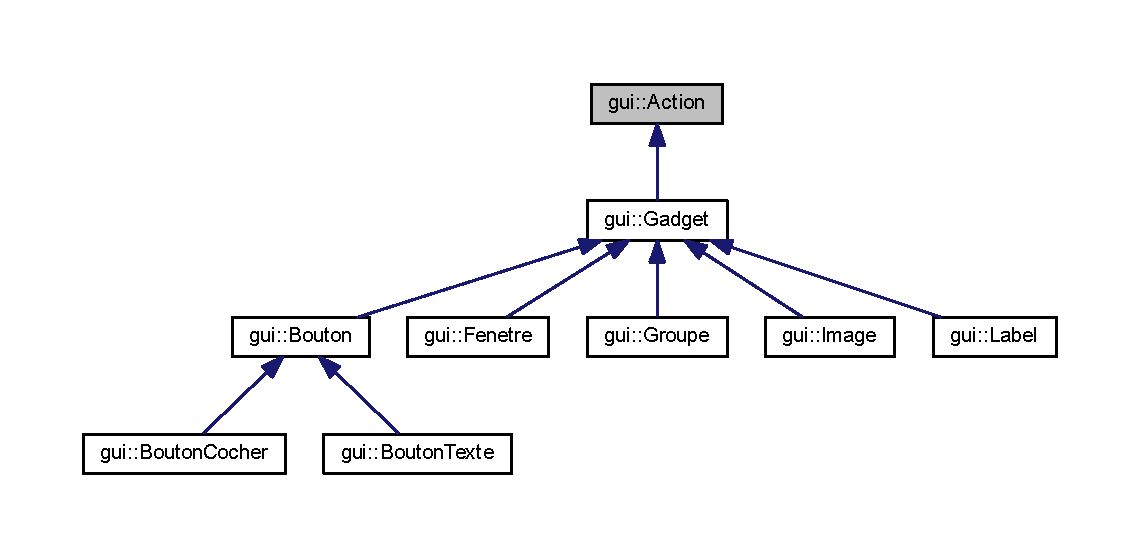
\includegraphics[width=350pt]{classgui_1_1_action__inherit__graph}
\end{center}
\end{figure}
\subsection*{Types publics}
\begin{DoxyCompactItemize}
\item 
using {\bf Func\+Type} = std\+::function$<$ void()$>$
\begin{DoxyCompactList}\small\item\em la fonction lambda associé aux declenchements des evenements. \end{DoxyCompactList}\item 
typedef std\+::map$<$ sf\+::\+Keyboard\+::\+Key, {\bf Func\+Type} $>$ {\bf evt\+Clavier}
\begin{DoxyCompactList}\small\item\em Collecteur d\textquotesingle{}évenements clavier. \end{DoxyCompactList}\item 
typedef std\+::map$<$ {\bf Evenements}, {\bf Func\+Type} $>$ {\bf evt\+Souris}
\begin{DoxyCompactList}\small\item\em collecteur d\textquotesingle{}évenement déclenché par nos \doxyref{gui\+::\+Evenements}{p.}{namespacegui_a679a250c68f3a4f70b52673ccf7c843e} (souris, fenetre ..) \end{DoxyCompactList}\end{DoxyCompactItemize}
\subsection*{Fonctions membres publiques}
\begin{DoxyCompactItemize}
\item 
virtual void {\bf lier} ({\bf Evenements} evt, const {\bf Func\+Type} \&fonction)
\begin{DoxyCompactList}\small\item\em Ajoute un ecouteur d\textquotesingle{}evenement associé à une fonction lambda(\+Func\+Type) à executer lors du déclenchement de l\textquotesingle{}evenement. \end{DoxyCompactList}\item 
virtual void {\bf lier} (sf\+::\+Keyboard\+::\+Key touche, const {\bf Func\+Type} \&fonction)
\begin{DoxyCompactList}\small\item\em Ajoute un ecouteur d\textquotesingle{}evenement associé à une fonction lambda(\+Func\+Type) à executer lors du déclenchement de l\textquotesingle{}evenement. \end{DoxyCompactList}\item 
virtual void {\bf delier} ({\bf Evenements} evt)
\begin{DoxyCompactList}\small\item\em supprimer un ecouteur d\textquotesingle{}évenement. \end{DoxyCompactList}\item 
virtual void {\bf delier} (sf\+::\+Keyboard\+::\+Key touche)
\begin{DoxyCompactList}\small\item\em supprimer un ecouteur d\textquotesingle{}évenement clavier. \end{DoxyCompactList}\end{DoxyCompactItemize}
\subsection*{Attributs publics statiques}
\begin{DoxyCompactItemize}
\item 
static {\bf Func\+Type} {\bf default\+Func} = [$\,$]( )-\/$>$void\{\}
\begin{DoxyCompactList}\small\item\em type par defaut de la fonction lambda. \end{DoxyCompactList}\end{DoxyCompactItemize}
\subsection*{Fonctions membres protégées}
\begin{DoxyCompactItemize}
\item 
void {\bf declencher} ({\bf Evenements} evt)
\begin{DoxyCompactList}\small\item\em Déclencher la fonction associé à l\textquotesingle{}évenement. \end{DoxyCompactList}\item 
bool {\bf traiter\+\_\+evenements} (const sf\+::\+Event \&event)
\begin{DoxyCompactList}\small\item\em La gestion des évènements utilisateurs. \end{DoxyCompactList}\end{DoxyCompactItemize}
\subsection*{Attributs protégés}
\begin{DoxyCompactItemize}
\item 
{\bf evt\+Souris} {\bf \+\_\+evts\+Souris}
\begin{DoxyCompactList}\small\item\em La liste des evenements souris enregistrés. \end{DoxyCompactList}\item 
{\bf evt\+Clavier} {\bf \+\_\+evts\+Clavier}
\begin{DoxyCompactList}\small\item\em La liste des evenements Claviers enregistrés. \end{DoxyCompactList}\end{DoxyCompactItemize}


\subsection{Description détaillée}
Classe virtuelle permetant de lier des évenements à des fonctions. 

Gère les évenements, permet de déclencher des fonctions associées à des évènements ...

\begin{DoxySeeAlso}{Voir également}
sf\+::\+Shape, sf\+::\+Circle\+Shape, sf\+::\+Convex\+Shape 
\end{DoxySeeAlso}


\subsection{Documentation des définitions de type membres}
\index{gui\+::\+Action@{gui\+::\+Action}!evt\+Clavier@{evt\+Clavier}}
\index{evt\+Clavier@{evt\+Clavier}!gui\+::\+Action@{gui\+::\+Action}}
\subsubsection[{evt\+Clavier}]{\setlength{\rightskip}{0pt plus 5cm}typedef std\+::map$<$ sf\+::\+Keyboard\+::\+Key , {\bf Func\+Type} $>$ {\bf gui\+::\+Action\+::evt\+Clavier}}\label{classgui_1_1_action_a7a85a606811b45e6232414b1d4e29bed}


Collecteur d\textquotesingle{}évenements clavier. 

\index{gui\+::\+Action@{gui\+::\+Action}!evt\+Souris@{evt\+Souris}}
\index{evt\+Souris@{evt\+Souris}!gui\+::\+Action@{gui\+::\+Action}}
\subsubsection[{evt\+Souris}]{\setlength{\rightskip}{0pt plus 5cm}typedef std\+::map$<$ {\bf Evenements} , {\bf Func\+Type} $>$ {\bf gui\+::\+Action\+::evt\+Souris}}\label{classgui_1_1_action_a359295e3ccae6767582f4450b6c49ec4}


collecteur d\textquotesingle{}évenement déclenché par nos \doxyref{gui\+::\+Evenements}{p.}{namespacegui_a679a250c68f3a4f70b52673ccf7c843e} (souris, fenetre ..) 

\index{gui\+::\+Action@{gui\+::\+Action}!Func\+Type@{Func\+Type}}
\index{Func\+Type@{Func\+Type}!gui\+::\+Action@{gui\+::\+Action}}
\subsubsection[{Func\+Type}]{\setlength{\rightskip}{0pt plus 5cm}using {\bf gui\+::\+Action\+::\+Func\+Type} =  std\+::function$<$void()$>$}\label{classgui_1_1_action_a4223568d083f940e94c80829f63ae817}


la fonction lambda associé aux declenchements des evenements. 



\subsection{Documentation des fonctions membres}
\index{gui\+::\+Action@{gui\+::\+Action}!declencher@{declencher}}
\index{declencher@{declencher}!gui\+::\+Action@{gui\+::\+Action}}
\subsubsection[{declencher(\+Evenements evt)}]{\setlength{\rightskip}{0pt plus 5cm}void gui\+::\+Action\+::declencher (
\begin{DoxyParamCaption}
\item[{{\bf Evenements}}]{evt}
\end{DoxyParamCaption}
)\hspace{0.3cm}{\ttfamily [protected]}}\label{classgui_1_1_action_aa7481b3efcebd774ad68bf1a4308041a}


Déclencher la fonction associé à l\textquotesingle{}évenement. 


\begin{DoxyParams}{Paramètres}
{\em evt} & L\textquotesingle{}evenement souris à declencher. \\
\hline
\end{DoxyParams}
\begin{DoxyReturn}{Renvoie}
Rien. 
\end{DoxyReturn}


Voici le graphe des appelants de cette fonction \+:\nopagebreak
\begin{figure}[H]
\begin{center}
\leavevmode
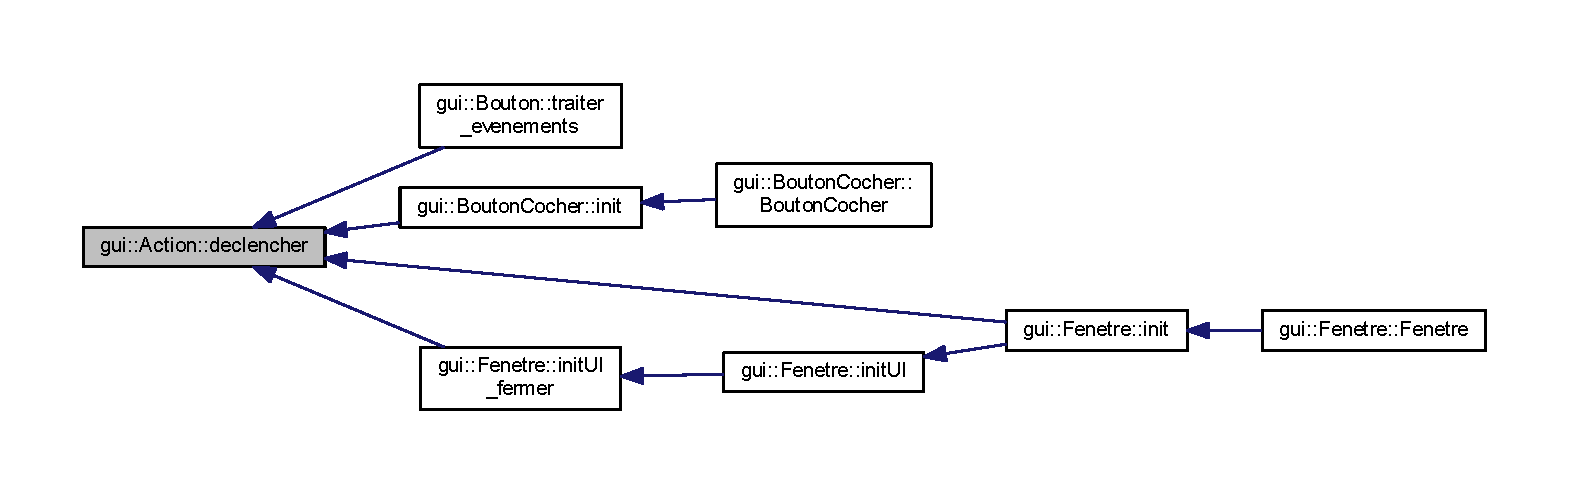
\includegraphics[width=350pt]{classgui_1_1_action_aa7481b3efcebd774ad68bf1a4308041a_icgraph}
\end{center}
\end{figure}


\index{gui\+::\+Action@{gui\+::\+Action}!delier@{delier}}
\index{delier@{delier}!gui\+::\+Action@{gui\+::\+Action}}
\subsubsection[{delier(\+Evenements evt)}]{\setlength{\rightskip}{0pt plus 5cm}void gui\+::\+Action\+::delier (
\begin{DoxyParamCaption}
\item[{{\bf Evenements}}]{evt}
\end{DoxyParamCaption}
)\hspace{0.3cm}{\ttfamily [virtual]}}\label{classgui_1_1_action_a2e82dcc2a557564140171006f21b6739}


supprimer un ecouteur d\textquotesingle{}évenement. 


\begin{DoxyParams}{Paramètres}
{\em evt} & Un evenement souris de la liste \+\_\+evts\+Souris.. \\
\hline
\end{DoxyParams}
\begin{DoxyReturn}{Renvoie}
Rien. 
\end{DoxyReturn}
\index{gui\+::\+Action@{gui\+::\+Action}!delier@{delier}}
\index{delier@{delier}!gui\+::\+Action@{gui\+::\+Action}}
\subsubsection[{delier(sf\+::\+Keyboard\+::\+Key touche)}]{\setlength{\rightskip}{0pt plus 5cm}void gui\+::\+Action\+::delier (
\begin{DoxyParamCaption}
\item[{sf\+::\+Keyboard\+::\+Key}]{touche}
\end{DoxyParamCaption}
)\hspace{0.3cm}{\ttfamily [virtual]}}\label{classgui_1_1_action_a588807ec36e45f27c2520de5a1e22aed}


supprimer un ecouteur d\textquotesingle{}évenement clavier. 


\begin{DoxyParams}{Paramètres}
{\em touche} & Une touche du clavier sf\+::\+Keyboard\+::\+Key. \\
\hline
\end{DoxyParams}
\begin{DoxyReturn}{Renvoie}
Rien. 
\end{DoxyReturn}
\index{gui\+::\+Action@{gui\+::\+Action}!lier@{lier}}
\index{lier@{lier}!gui\+::\+Action@{gui\+::\+Action}}
\subsubsection[{lier(\+Evenements evt, const Func\+Type \&fonction)}]{\setlength{\rightskip}{0pt plus 5cm}void gui\+::\+Action\+::lier (
\begin{DoxyParamCaption}
\item[{{\bf Evenements}}]{evt, }
\item[{const {\bf Func\+Type} \&}]{fonction}
\end{DoxyParamCaption}
)\hspace{0.3cm}{\ttfamily [virtual]}}\label{classgui_1_1_action_a70035bc714f01d2f47c58b4dc159fb32}


Ajoute un ecouteur d\textquotesingle{}evenement associé à une fonction lambda(\+Func\+Type) à executer lors du déclenchement de l\textquotesingle{}evenement. 


\begin{DoxyParams}{Paramètres}
{\em evt} & Un evenement de la liste Evenements. \\
\hline
{\em fonction} & la fonction lambda associé. \\
\hline
\end{DoxyParams}
\begin{DoxyReturn}{Renvoie}
Rien. 
\end{DoxyReturn}


Voici le graphe des appelants de cette fonction \+:\nopagebreak
\begin{figure}[H]
\begin{center}
\leavevmode
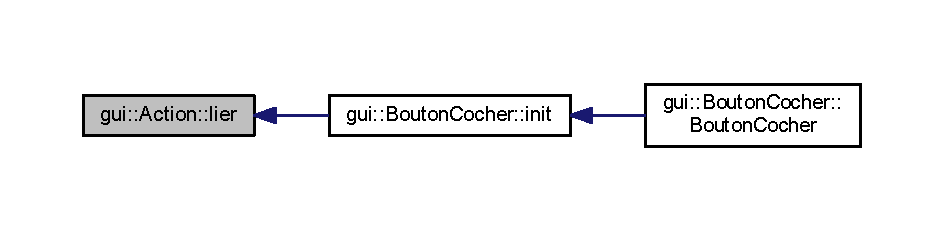
\includegraphics[width=350pt]{classgui_1_1_action_a70035bc714f01d2f47c58b4dc159fb32_icgraph}
\end{center}
\end{figure}


\index{gui\+::\+Action@{gui\+::\+Action}!lier@{lier}}
\index{lier@{lier}!gui\+::\+Action@{gui\+::\+Action}}
\subsubsection[{lier(sf\+::\+Keyboard\+::\+Key touche, const Func\+Type \&fonction)}]{\setlength{\rightskip}{0pt plus 5cm}void gui\+::\+Action\+::lier (
\begin{DoxyParamCaption}
\item[{sf\+::\+Keyboard\+::\+Key}]{touche, }
\item[{const {\bf Func\+Type} \&}]{fonction}
\end{DoxyParamCaption}
)\hspace{0.3cm}{\ttfamily [virtual]}}\label{classgui_1_1_action_a5eb8461689c5b9800c3b652423dc53d3}


Ajoute un ecouteur d\textquotesingle{}evenement associé à une fonction lambda(\+Func\+Type) à executer lors du déclenchement de l\textquotesingle{}evenement. 


\begin{DoxyParams}{Paramètres}
{\em touche} & Une touche du clavier sf\+::\+Keyboard\+::\+Key. \\
\hline
{\em fonction} & la fonction lambda associé. \\
\hline
\end{DoxyParams}
\begin{DoxyReturn}{Renvoie}
Rien. 
\end{DoxyReturn}
\index{gui\+::\+Action@{gui\+::\+Action}!traiter\+\_\+evenements@{traiter\+\_\+evenements}}
\index{traiter\+\_\+evenements@{traiter\+\_\+evenements}!gui\+::\+Action@{gui\+::\+Action}}
\subsubsection[{traiter\+\_\+evenements(const sf\+::\+Event \&event)}]{\setlength{\rightskip}{0pt plus 5cm}bool gui\+::\+Action\+::traiter\+\_\+evenements (
\begin{DoxyParamCaption}
\item[{const sf\+::\+Event \&}]{event}
\end{DoxyParamCaption}
)\hspace{0.3cm}{\ttfamily [protected]}}\label{classgui_1_1_action_a7c0cd2dd198d840342cbd6b0ac193a02}


La gestion des évènements utilisateurs. 


\begin{DoxyParams}{Paramètres}
{\em event} & les évènements claviers \\
\hline
\end{DoxyParams}
\begin{DoxyReturn}{Renvoie}
Rien 
\end{DoxyReturn}


Voici le graphe des appelants de cette fonction \+:\nopagebreak
\begin{figure}[H]
\begin{center}
\leavevmode
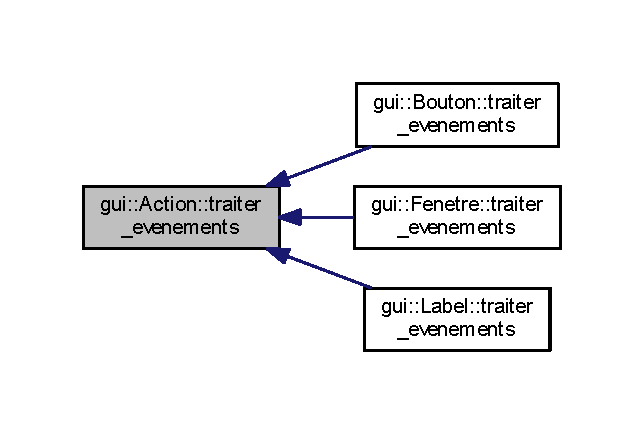
\includegraphics[width=309pt]{classgui_1_1_action_a7c0cd2dd198d840342cbd6b0ac193a02_icgraph}
\end{center}
\end{figure}




\subsection{Documentation des champs}
\index{gui\+::\+Action@{gui\+::\+Action}!\+\_\+evts\+Clavier@{\+\_\+evts\+Clavier}}
\index{\+\_\+evts\+Clavier@{\+\_\+evts\+Clavier}!gui\+::\+Action@{gui\+::\+Action}}
\subsubsection[{\+\_\+evts\+Clavier}]{\setlength{\rightskip}{0pt plus 5cm}{\bf evt\+Clavier} gui\+::\+Action\+::\+\_\+evts\+Clavier\hspace{0.3cm}{\ttfamily [protected]}}\label{classgui_1_1_action_acb4c5836898b8221986f90a5b226908e}


La liste des evenements Claviers enregistrés. 

\index{gui\+::\+Action@{gui\+::\+Action}!\+\_\+evts\+Souris@{\+\_\+evts\+Souris}}
\index{\+\_\+evts\+Souris@{\+\_\+evts\+Souris}!gui\+::\+Action@{gui\+::\+Action}}
\subsubsection[{\+\_\+evts\+Souris}]{\setlength{\rightskip}{0pt plus 5cm}{\bf evt\+Souris} gui\+::\+Action\+::\+\_\+evts\+Souris\hspace{0.3cm}{\ttfamily [protected]}}\label{classgui_1_1_action_ae3dfea6e15a336d6095fcddeccee27ac}


La liste des evenements souris enregistrés. 

\index{gui\+::\+Action@{gui\+::\+Action}!default\+Func@{default\+Func}}
\index{default\+Func@{default\+Func}!gui\+::\+Action@{gui\+::\+Action}}
\subsubsection[{default\+Func}]{\setlength{\rightskip}{0pt plus 5cm}{\bf Action\+::\+Func\+Type} gui\+::\+Action\+::default\+Func = [$\,$]( )-\/$>$void\{\}\hspace{0.3cm}{\ttfamily [static]}}\label{classgui_1_1_action_a7338e98b0107777d8168bb12a021167b}


type par defaut de la fonction lambda. 



La documentation de cette classe a été générée à partir des fichiers suivants \+:\begin{DoxyCompactItemize}
\item 
Interface/include/{\bf Action.\+h}\item 
Interface/src/{\bf Action.\+cpp}\end{DoxyCompactItemize}

\section{Référence de la classe app\+:\+:Application}
\label{classapp_1_1_application}\index{app\+::\+Application@{app\+::\+Application}}


La classe de base du programme.  




{\ttfamily \#include $<$Application.\+h$>$}



Graphe de collaboration de app\+:\+:Application\+:\nopagebreak
\begin{figure}[H]
\begin{center}
\leavevmode
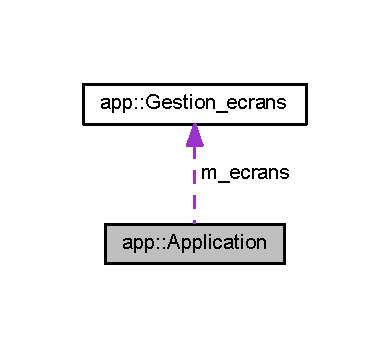
\includegraphics[width=187pt]{classapp_1_1_application__coll__graph}
\end{center}
\end{figure}
\subsection*{Fonctions membres publiques}
\begin{DoxyCompactItemize}
\item 
{\bf Application} ()
\begin{DoxyCompactList}\small\item\em Constructeur. \end{DoxyCompactList}\item 
virtual {\bf $\sim$\+Application} ()
\begin{DoxyCompactList}\small\item\em Destructeur. \end{DoxyCompactList}\item 
void {\bf executer} ()
\begin{DoxyCompactList}\small\item\em La boucle principale. \end{DoxyCompactList}\item 
void {\bf traiter\+\_\+evenements} ()
\begin{DoxyCompactList}\small\item\em La gestion des évènements utilisateurs. \end{DoxyCompactList}\item 
void {\bf actualiser} (float delta\+T)
\begin{DoxyCompactList}\small\item\em Actualiser les éléments. \end{DoxyCompactList}\item 
void {\bf dessiner} ()
\begin{DoxyCompactList}\small\item\em Rendre les éléments. \end{DoxyCompactList}\item 
sf\+::\+Render\+Window \& {\bf get\+Fenetre} ()
\begin{DoxyCompactList}\small\item\em renvois la fenetre sfml de l\textquotesingle{}application \end{DoxyCompactList}\end{DoxyCompactItemize}
\subsection*{Attributs privés}
\begin{DoxyCompactItemize}
\item 
{\bf Gestion\+\_\+ecrans} {\bf m\+\_\+ecrans}
\begin{DoxyCompactList}\small\item\em Le gestionnaire des écrans. \end{DoxyCompactList}\item 
sf\+::\+Render\+Window {\bf m\+\_\+fenetre}
\begin{DoxyCompactList}\small\item\em La fenêtre S\+F\+M\+L. \end{DoxyCompactList}\end{DoxyCompactItemize}


\subsection{Description détaillée}
La classe de base du programme. 

\subsection{Documentation des constructeurs et destructeur}
\index{app\+::\+Application@{app\+::\+Application}!Application@{Application}}
\index{Application@{Application}!app\+::\+Application@{app\+::\+Application}}
\subsubsection[{Application()}]{\setlength{\rightskip}{0pt plus 5cm}app\+::\+Application\+::\+Application (
\begin{DoxyParamCaption}
{}
\end{DoxyParamCaption}
)}\label{classapp_1_1_application_a3c480be05f51b91e648b2f6533a32f1b}


Constructeur. 



Voici le graphe d\textquotesingle{}appel pour cette fonction \+:\nopagebreak
\begin{figure}[H]
\begin{center}
\leavevmode
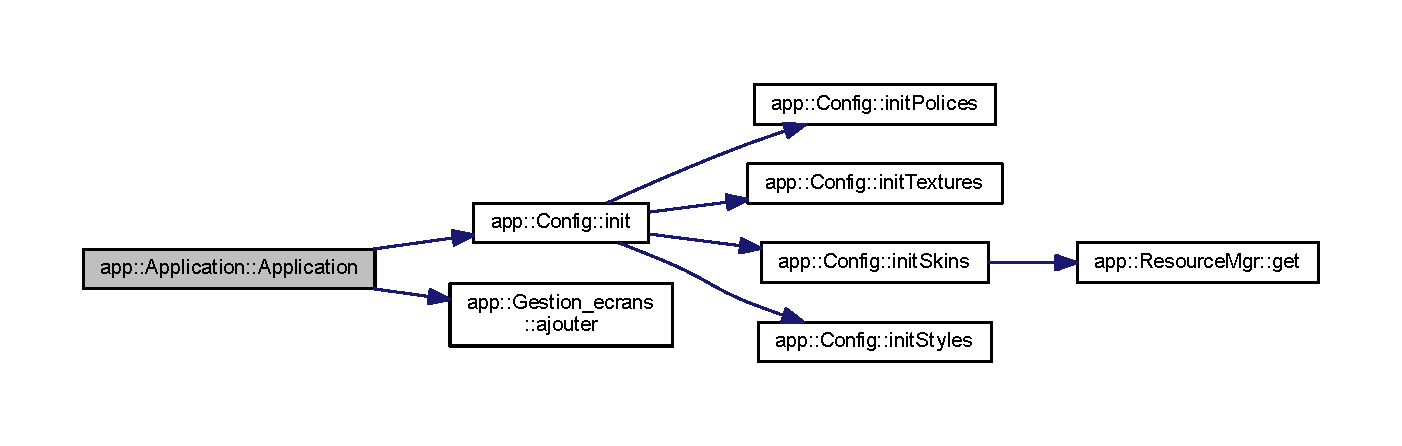
\includegraphics[width=350pt]{classapp_1_1_application_a3c480be05f51b91e648b2f6533a32f1b_cgraph}
\end{center}
\end{figure}


\index{app\+::\+Application@{app\+::\+Application}!````~Application@{$\sim$\+Application}}
\index{````~Application@{$\sim$\+Application}!app\+::\+Application@{app\+::\+Application}}
\subsubsection[{$\sim$\+Application()}]{\setlength{\rightskip}{0pt plus 5cm}app\+::\+Application\+::$\sim$\+Application (
\begin{DoxyParamCaption}
{}
\end{DoxyParamCaption}
)\hspace{0.3cm}{\ttfamily [virtual]}}\label{classapp_1_1_application_addde1f674adf0f1d2cc4697e36f7c9e3}


Destructeur. 



Voici le graphe d\textquotesingle{}appel pour cette fonction \+:\nopagebreak
\begin{figure}[H]
\begin{center}
\leavevmode
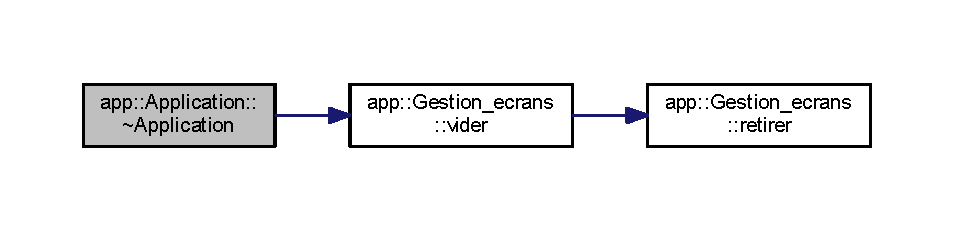
\includegraphics[width=350pt]{classapp_1_1_application_addde1f674adf0f1d2cc4697e36f7c9e3_cgraph}
\end{center}
\end{figure}




\subsection{Documentation des fonctions membres}
\index{app\+::\+Application@{app\+::\+Application}!actualiser@{actualiser}}
\index{actualiser@{actualiser}!app\+::\+Application@{app\+::\+Application}}
\subsubsection[{actualiser(float delta\+T)}]{\setlength{\rightskip}{0pt plus 5cm}void app\+::\+Application\+::actualiser (
\begin{DoxyParamCaption}
\item[{float}]{delta\+T}
\end{DoxyParamCaption}
)}\label{classapp_1_1_application_a1b728d3f1b0717dee8d4e4190df1cd65}


Actualiser les éléments. 

Actualiser les différents éléments du ou des écrans actifs. 
\begin{DoxyParams}{Paramètres}
{\em delta\+T} & Un {\itshape float} qui indique le delta du temps écoulé depuis la dernière actualisation. ca permet quand on actualise de ponderer les mouvement en fonction du temps et ainsi avoir une indépendance entre animation et frame rate. \\
\hline
\end{DoxyParams}
\begin{DoxyReturn}{Renvoie}
Rien 
\end{DoxyReturn}


Voici le graphe d\textquotesingle{}appel pour cette fonction \+:\nopagebreak
\begin{figure}[H]
\begin{center}
\leavevmode
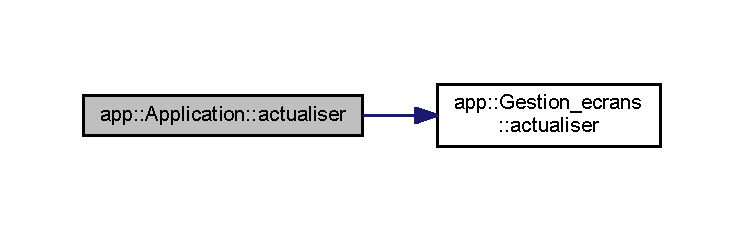
\includegraphics[width=350pt]{classapp_1_1_application_a1b728d3f1b0717dee8d4e4190df1cd65_cgraph}
\end{center}
\end{figure}




Voici le graphe des appelants de cette fonction \+:\nopagebreak
\begin{figure}[H]
\begin{center}
\leavevmode
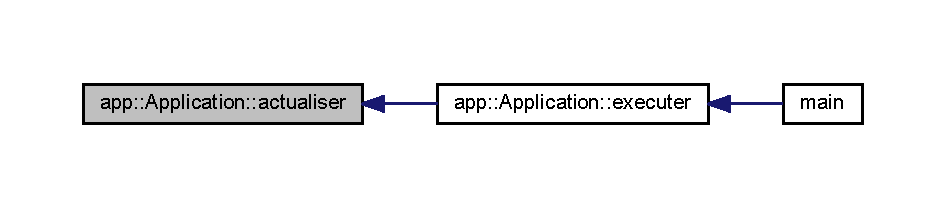
\includegraphics[width=350pt]{classapp_1_1_application_a1b728d3f1b0717dee8d4e4190df1cd65_icgraph}
\end{center}
\end{figure}


\index{app\+::\+Application@{app\+::\+Application}!dessiner@{dessiner}}
\index{dessiner@{dessiner}!app\+::\+Application@{app\+::\+Application}}
\subsubsection[{dessiner()}]{\setlength{\rightskip}{0pt plus 5cm}void app\+::\+Application\+::dessiner (
\begin{DoxyParamCaption}
{}
\end{DoxyParamCaption}
)}\label{classapp_1_1_application_a03b3bac56e523faa9669622eadd237f8}


Rendre les éléments. 

Dessiner les différents éléments du ou des écrans actifs. \begin{DoxyReturn}{Renvoie}
Rien 
\end{DoxyReturn}
\begin{quote}
Vider la fenetre. \end{quote}


\begin{quote}
Rendu des ecrans courants. \end{quote}


\begin{quote}
Afficher la fenêtre. \end{quote}


Voici le graphe d\textquotesingle{}appel pour cette fonction \+:\nopagebreak
\begin{figure}[H]
\begin{center}
\leavevmode
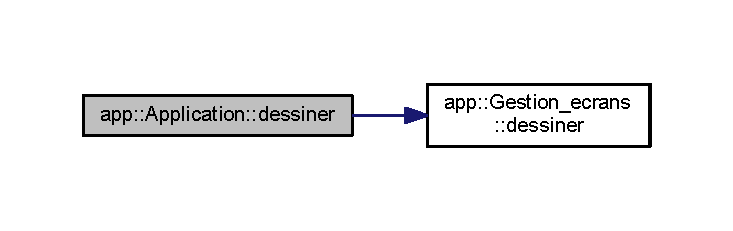
\includegraphics[width=350pt]{classapp_1_1_application_a03b3bac56e523faa9669622eadd237f8_cgraph}
\end{center}
\end{figure}




Voici le graphe des appelants de cette fonction \+:\nopagebreak
\begin{figure}[H]
\begin{center}
\leavevmode
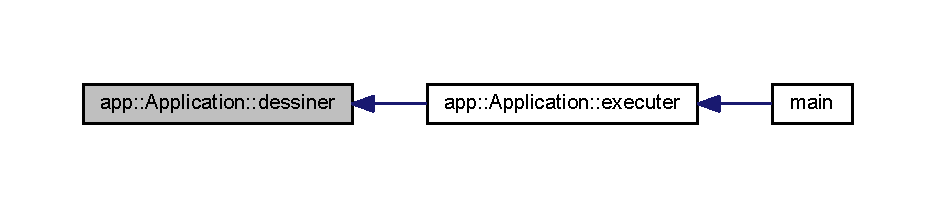
\includegraphics[width=350pt]{classapp_1_1_application_a03b3bac56e523faa9669622eadd237f8_icgraph}
\end{center}
\end{figure}


\index{app\+::\+Application@{app\+::\+Application}!executer@{executer}}
\index{executer@{executer}!app\+::\+Application@{app\+::\+Application}}
\subsubsection[{executer()}]{\setlength{\rightskip}{0pt plus 5cm}void app\+::\+Application\+::executer (
\begin{DoxyParamCaption}
{}
\end{DoxyParamCaption}
)}\label{classapp_1_1_application_ae375e0fdeb21265f93cff8958a26f95d}


La boucle principale. 

\begin{DoxyReturn}{Renvoie}
Rien 
\end{DoxyReturn}


Voici le graphe d\textquotesingle{}appel pour cette fonction \+:\nopagebreak
\begin{figure}[H]
\begin{center}
\leavevmode
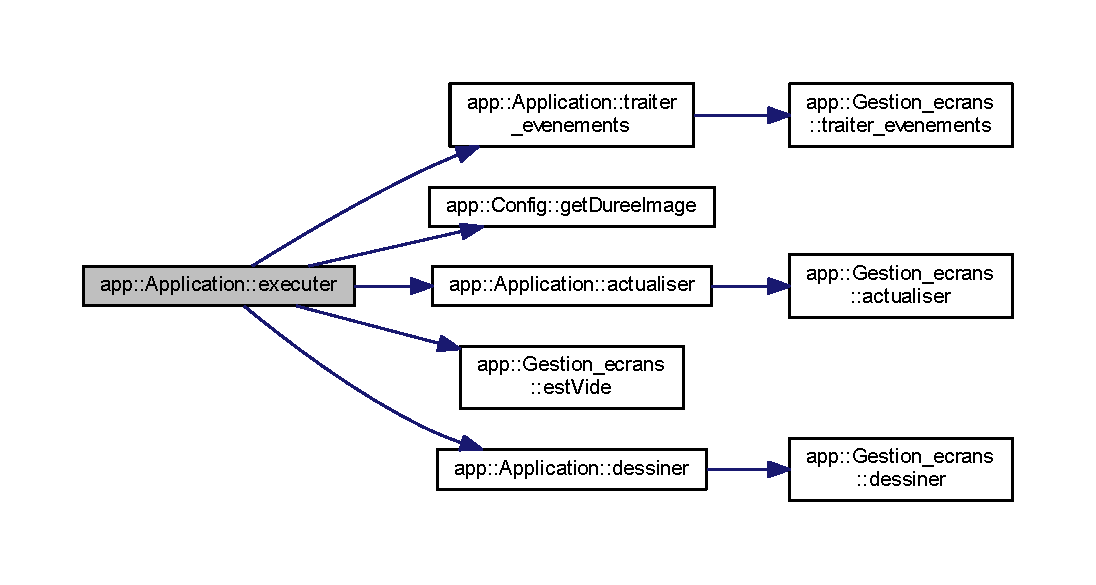
\includegraphics[width=350pt]{classapp_1_1_application_ae375e0fdeb21265f93cff8958a26f95d_cgraph}
\end{center}
\end{figure}




Voici le graphe des appelants de cette fonction \+:\nopagebreak
\begin{figure}[H]
\begin{center}
\leavevmode
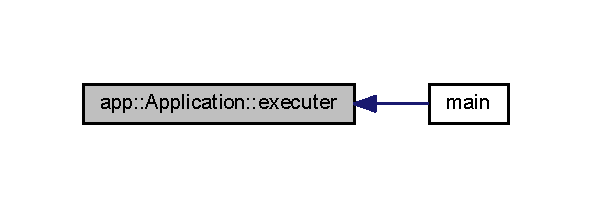
\includegraphics[width=284pt]{classapp_1_1_application_ae375e0fdeb21265f93cff8958a26f95d_icgraph}
\end{center}
\end{figure}


\index{app\+::\+Application@{app\+::\+Application}!get\+Fenetre@{get\+Fenetre}}
\index{get\+Fenetre@{get\+Fenetre}!app\+::\+Application@{app\+::\+Application}}
\subsubsection[{get\+Fenetre()}]{\setlength{\rightskip}{0pt plus 5cm}sf\+::\+Render\+Window \& app\+::\+Application\+::get\+Fenetre (
\begin{DoxyParamCaption}
{}
\end{DoxyParamCaption}
)}\label{classapp_1_1_application_acbc0a186b9ec7abfaf35eaad5d55b45a}


renvois la fenetre sfml de l\textquotesingle{}application 

\begin{DoxyReturn}{Renvoie}
la fenetre sfml de l\textquotesingle{}application 
\end{DoxyReturn}


Voici le graphe des appelants de cette fonction \+:\nopagebreak
\begin{figure}[H]
\begin{center}
\leavevmode
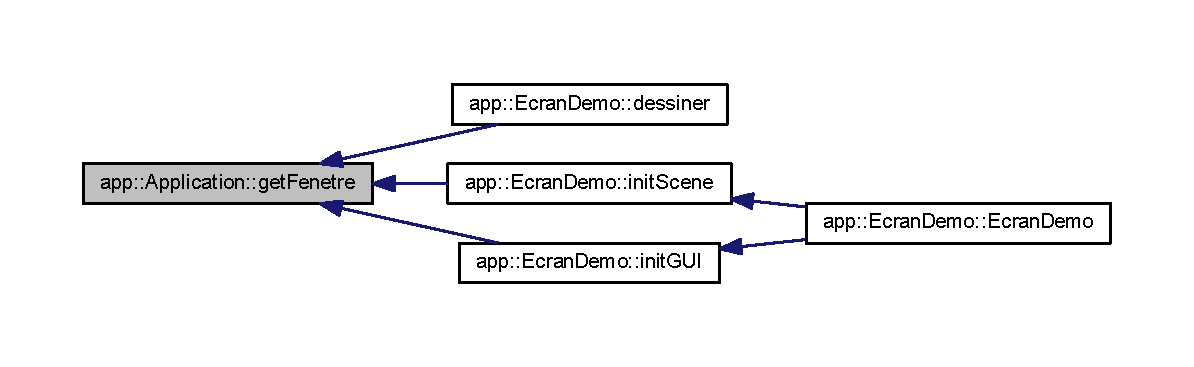
\includegraphics[width=350pt]{classapp_1_1_application_acbc0a186b9ec7abfaf35eaad5d55b45a_icgraph}
\end{center}
\end{figure}


\index{app\+::\+Application@{app\+::\+Application}!traiter\+\_\+evenements@{traiter\+\_\+evenements}}
\index{traiter\+\_\+evenements@{traiter\+\_\+evenements}!app\+::\+Application@{app\+::\+Application}}
\subsubsection[{traiter\+\_\+evenements()}]{\setlength{\rightskip}{0pt plus 5cm}void app\+::\+Application\+::traiter\+\_\+evenements (
\begin{DoxyParamCaption}
{}
\end{DoxyParamCaption}
)}\label{classapp_1_1_application_aee4bdeeb44c6b2a943acc8e651b0ff83}


La gestion des évènements utilisateurs. 

Gère les entrées claviers, souris, fenetre ... \begin{DoxyReturn}{Renvoie}
Rien 
\end{DoxyReturn}


Voici le graphe d\textquotesingle{}appel pour cette fonction \+:\nopagebreak
\begin{figure}[H]
\begin{center}
\leavevmode
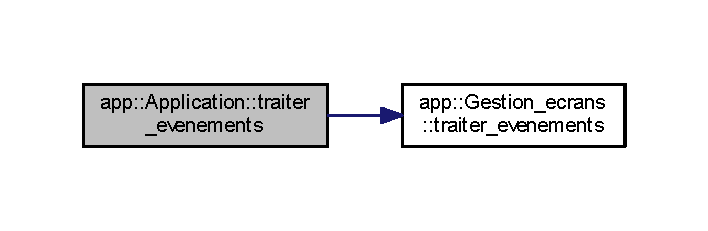
\includegraphics[width=340pt]{classapp_1_1_application_aee4bdeeb44c6b2a943acc8e651b0ff83_cgraph}
\end{center}
\end{figure}




Voici le graphe des appelants de cette fonction \+:\nopagebreak
\begin{figure}[H]
\begin{center}
\leavevmode
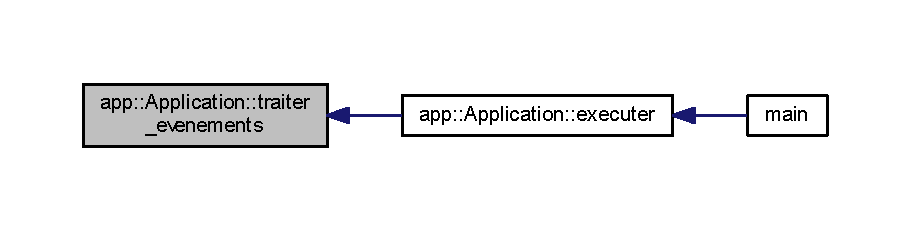
\includegraphics[width=350pt]{classapp_1_1_application_aee4bdeeb44c6b2a943acc8e651b0ff83_icgraph}
\end{center}
\end{figure}




\subsection{Documentation des champs}
\index{app\+::\+Application@{app\+::\+Application}!m\+\_\+ecrans@{m\+\_\+ecrans}}
\index{m\+\_\+ecrans@{m\+\_\+ecrans}!app\+::\+Application@{app\+::\+Application}}
\subsubsection[{m\+\_\+ecrans}]{\setlength{\rightskip}{0pt plus 5cm}{\bf Gestion\+\_\+ecrans} app\+::\+Application\+::m\+\_\+ecrans\hspace{0.3cm}{\ttfamily [private]}}\label{classapp_1_1_application_ae619078005ea4200ea4db019c0f6d8de}


Le gestionnaire des écrans. 

\index{app\+::\+Application@{app\+::\+Application}!m\+\_\+fenetre@{m\+\_\+fenetre}}
\index{m\+\_\+fenetre@{m\+\_\+fenetre}!app\+::\+Application@{app\+::\+Application}}
\subsubsection[{m\+\_\+fenetre}]{\setlength{\rightskip}{0pt plus 5cm}sf\+::\+Render\+Window app\+::\+Application\+::m\+\_\+fenetre\hspace{0.3cm}{\ttfamily [private]}}\label{classapp_1_1_application_a2b45d94b25a7b29cb7409b7701c3c2d5}


La fenêtre S\+F\+M\+L. 



La documentation de cette classe a été générée à partir des fichiers suivants \+:\begin{DoxyCompactItemize}
\item 
main/include/{\bf Application.\+h}\item 
main/src/{\bf Application.\+cpp}\end{DoxyCompactItemize}

\section{Référence de la classe gui\+:\+:Bouton}
\label{classgui_1_1_bouton}\index{gui\+::\+Bouton@{gui\+::\+Bouton}}


\doxyref{Gadget}{p.}{classgui_1_1_gadget}, simple bouton rectangulaire.  




{\ttfamily \#include $<$Bouton.\+h$>$}



Graphe d\textquotesingle{}héritage de gui\+:\+:Bouton\+:\nopagebreak
\begin{figure}[H]
\begin{center}
\leavevmode
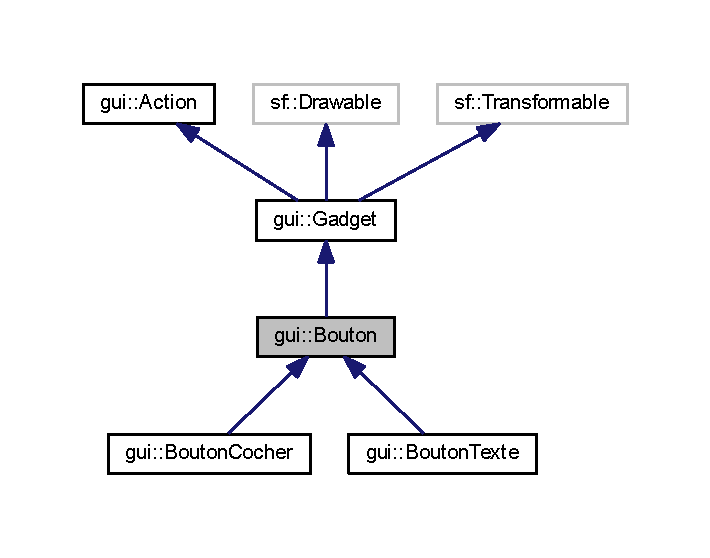
\includegraphics[width=341pt]{classgui_1_1_bouton__inherit__graph}
\end{center}
\end{figure}


Graphe de collaboration de gui\+:\+:Bouton\+:\nopagebreak
\begin{figure}[H]
\begin{center}
\leavevmode
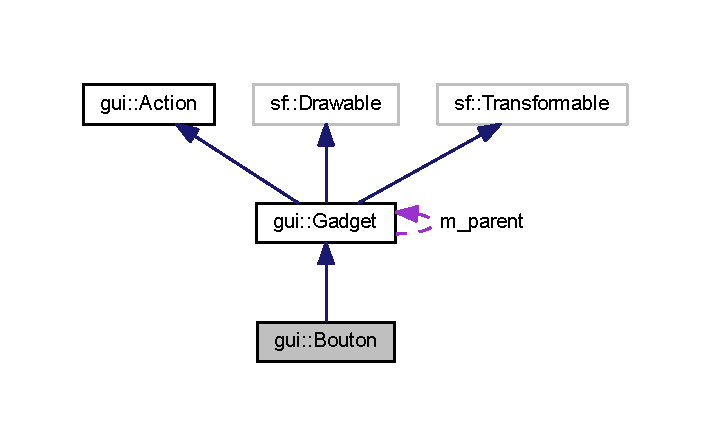
\includegraphics[width=341pt]{classgui_1_1_bouton__coll__graph}
\end{center}
\end{figure}
\subsection*{Types publics}
\begin{DoxyCompactItemize}
\item 
enum {\bf Etat\+Bouton} \{ {\bf desactive}, 
{\bf repos}, 
{\bf survol}, 
{\bf press}
 \}\begin{DoxyCompactList}\small\item\em Les Différents états du gadget. \end{DoxyCompactList}
\end{DoxyCompactItemize}
\subsection*{Fonctions membres publiques}
\begin{DoxyCompactItemize}
\item 
{\bf Bouton} ()
\begin{DoxyCompactList}\small\item\em Constructeur par défaut. \end{DoxyCompactList}\item 
{\bf Bouton} (std\+::shared\+\_\+ptr$<$ {\bf Skin} $>$ skin)
\begin{DoxyCompactList}\small\item\em Constructeur en definisant un style. \end{DoxyCompactList}\item 
virtual {\bf $\sim$\+Bouton} ()
\begin{DoxyCompactList}\small\item\em Destructeur. \end{DoxyCompactList}\item 
virtual void {\bf set\+Size} (sf\+::\+Vector2f taille)
\begin{DoxyCompactList}\small\item\em Definir la taille du bouton. \end{DoxyCompactList}\item 
virtual sf\+::\+Vector2f {\bf get\+Size} ()
\begin{DoxyCompactList}\small\item\em Accesseur de la taille. \end{DoxyCompactList}\item 
virtual sf\+::\+Float\+Rect {\bf get\+Local\+Bounds} ()
\begin{DoxyCompactList}\small\item\em Accesseur de la bounding\+Box en local. \end{DoxyCompactList}\item 
virtual sf\+::\+Float\+Rect {\bf get\+Global\+Bounds} ()
\begin{DoxyCompactList}\small\item\em Accesseur de la bounding\+Box en global. \end{DoxyCompactList}\item 
virtual void {\bf set\+Fill\+Color} (sf\+::\+Color color)
\begin{DoxyCompactList}\small\item\em Definir Couleur du fond. \end{DoxyCompactList}\item 
virtual void {\bf set\+Outline\+Color} (sf\+::\+Color color)
\begin{DoxyCompactList}\small\item\em Definir Couleur du cadre. \end{DoxyCompactList}\item 
virtual void {\bf set\+Outline\+Thickness} (float epaisseur)
\begin{DoxyCompactList}\small\item\em Definir l\textquotesingle{}épaisseur du cadre. \end{DoxyCompactList}\item 
virtual void {\bf set\+Skin} (std\+::shared\+\_\+ptr$<$ {\bf Skin} $>$ skin)
\begin{DoxyCompactList}\small\item\em Définie le skin du \doxyref{Label}{p.}{classgui_1_1_label}. \end{DoxyCompactList}\item 
void {\bf set\+Bordure} (float val)
\begin{DoxyCompactList}\small\item\em Definir la bordure du texte. \end{DoxyCompactList}\item 
float {\bf get\+Bordure} ()
\begin{DoxyCompactList}\small\item\em Acceder à la bordure du bouton. \end{DoxyCompactList}\item 
virtual void {\bf traiter\+\_\+evenements} (const sf\+::\+Event \&event)
\begin{DoxyCompactList}\small\item\em La gestion des évènements utilisateurs. \end{DoxyCompactList}\item 
virtual void {\bf actualiser} (float delta\+T) override
\begin{DoxyCompactList}\small\item\em Actualiser les éléments. \end{DoxyCompactList}\item 
virtual void {\bf draw} (sf\+::\+Render\+Target \&target, sf\+::\+Render\+States states) const 
\begin{DoxyCompactList}\small\item\em Rendre les différents éléments du ou des écrans actifs. \end{DoxyCompactList}\end{DoxyCompactItemize}
\subsection*{Fonctions membres protégées}
\begin{DoxyCompactItemize}
\item 
virtual void {\bf maj\+Geom} ()
\begin{DoxyCompactList}\small\item\em Actualise le style du label. \end{DoxyCompactList}\end{DoxyCompactItemize}
\subsection*{Attributs protégés}
\begin{DoxyCompactItemize}
\item 
{\bf Etat\+Bouton} {\bf m\+\_\+etat}
\begin{DoxyCompactList}\small\item\em L\textquotesingle{}état du bouton. \end{DoxyCompactList}\item 
{\bf Etat\+Bouton} {\bf m\+\_\+etat\+Back}
\begin{DoxyCompactList}\small\item\em L\textquotesingle{}état du bouton la frame d\textquotesingle{}avant, pour verifier si changement d\textquotesingle{}état. \end{DoxyCompactList}\item 
std\+::shared\+\_\+ptr$<$ {\bf Image} $>$ {\bf m\+\_\+fond}
\begin{DoxyCompactList}\small\item\em Le rectangle du fond du bouton. \end{DoxyCompactList}\item 
sf\+::\+Clock {\bf m\+\_\+clock\+\_\+dbl\+Clique}
\begin{DoxyCompactList}\small\item\em Compteur temps pour double clique. \end{DoxyCompactList}\item 
bool {\bf m\+\_\+1er\+Click}
\begin{DoxyCompactList}\small\item\em bool double clique, true lors du 1er clique, false a la fin du temps ou apres second clique. \end{DoxyCompactList}\item 
float {\bf m\+\_\+bordure}
\begin{DoxyCompactList}\small\item\em l\textquotesingle{}espace de bordure (pour gui\+::bouton\+Texte, gui\+::\+Bouton\+Coher ..). \end{DoxyCompactList}\end{DoxyCompactItemize}
\subsection*{Membres hérités additionnels}


\subsection{Description détaillée}
\doxyref{Gadget}{p.}{classgui_1_1_gadget}, simple bouton rectangulaire. 

\begin{DoxyRefDesc}{A faire}
\item[{\bf A faire}]à résoudre \+:
\begin{DoxyItemize}
\item le relache hors du bouton s\textquotesingle{}active meme quand on a pas cliquer dessus avant.
\item pareil pour le double clique.
\end{DoxyItemize}\end{DoxyRefDesc}


exemple \+: 
\begin{DoxyCode}
\end{DoxyCode}
 \begin{DoxySeeAlso}{Voir également}
\doxyref{gui\+::\+Gadget}{p.}{classgui_1_1_gadget} 
\end{DoxySeeAlso}


\subsection{Documentation des énumérations membres}
\index{gui\+::\+Bouton@{gui\+::\+Bouton}!Etat\+Bouton@{Etat\+Bouton}}
\index{Etat\+Bouton@{Etat\+Bouton}!gui\+::\+Bouton@{gui\+::\+Bouton}}
\subsubsection[{Etat\+Bouton}]{\setlength{\rightskip}{0pt plus 5cm}enum {\bf gui\+::\+Bouton\+::\+Etat\+Bouton}}\label{classgui_1_1_bouton_a8c4622de7a2b734cb88c44d6b1caca5f}


Les Différents états du gadget. 

\begin{Desc}
\item[Valeurs énumérées]\par
\begin{description}
\index{desactive@{desactive}!gui\+::\+Bouton@{gui\+::\+Bouton}}\index{gui\+::\+Bouton@{gui\+::\+Bouton}!desactive@{desactive}}\item[{\em 
desactive\label{classgui_1_1_bouton_a8c4622de7a2b734cb88c44d6b1caca5fa0826242afa707857663ceb43c0484b4a}
}]visible mais inactif. \index{repos@{repos}!gui\+::\+Bouton@{gui\+::\+Bouton}}\index{gui\+::\+Bouton@{gui\+::\+Bouton}!repos@{repos}}\item[{\em 
repos\label{classgui_1_1_bouton_a8c4622de7a2b734cb88c44d6b1caca5fad0e5b1d339c41223ef5856f7663dd1c0}
}]en attente d\textquotesingle{}interaction. \index{survol@{survol}!gui\+::\+Bouton@{gui\+::\+Bouton}}\index{gui\+::\+Bouton@{gui\+::\+Bouton}!survol@{survol}}\item[{\em 
survol\label{classgui_1_1_bouton_a8c4622de7a2b734cb88c44d6b1caca5fa2b1991bff29414d4d3637d3641beba13}
}]quand la souris le survol. \index{press@{press}!gui\+::\+Bouton@{gui\+::\+Bouton}}\index{gui\+::\+Bouton@{gui\+::\+Bouton}!press@{press}}\item[{\em 
press\label{classgui_1_1_bouton_a8c4622de7a2b734cb88c44d6b1caca5fa960ca598786d4fe54aaeeaa55af90b5a}
}]quand un bouton est cliqué. \end{description}
\end{Desc}


\subsection{Documentation des constructeurs et destructeur}
\index{gui\+::\+Bouton@{gui\+::\+Bouton}!Bouton@{Bouton}}
\index{Bouton@{Bouton}!gui\+::\+Bouton@{gui\+::\+Bouton}}
\subsubsection[{Bouton()}]{\setlength{\rightskip}{0pt plus 5cm}gui\+::\+Bouton\+::\+Bouton (
\begin{DoxyParamCaption}
{}
\end{DoxyParamCaption}
)}\label{classgui_1_1_bouton_a98cf47d074d64c2915a24f3e9b76dfc7}


Constructeur par défaut. 



Voici le graphe d\textquotesingle{}appel pour cette fonction \+:\nopagebreak
\begin{figure}[H]
\begin{center}
\leavevmode
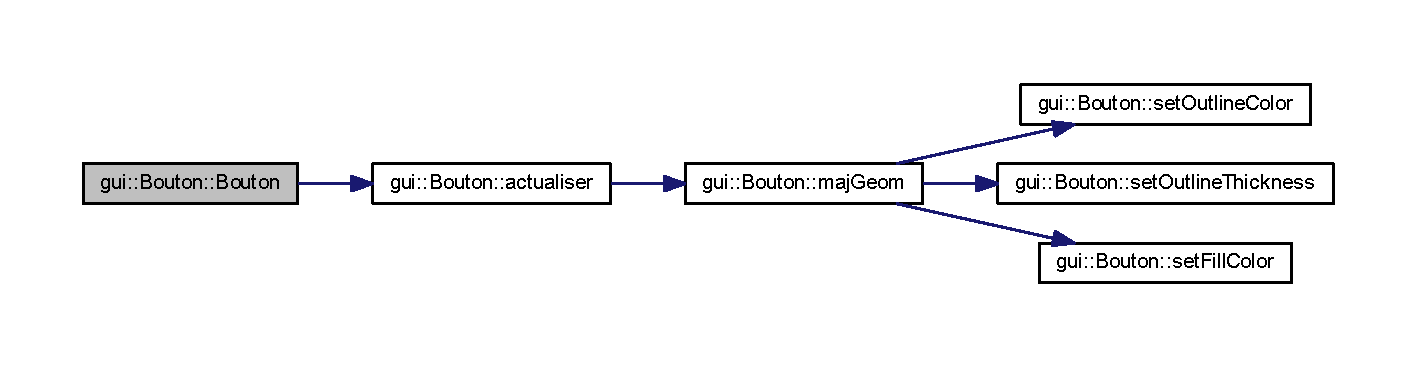
\includegraphics[width=350pt]{classgui_1_1_bouton_a98cf47d074d64c2915a24f3e9b76dfc7_cgraph}
\end{center}
\end{figure}


\index{gui\+::\+Bouton@{gui\+::\+Bouton}!Bouton@{Bouton}}
\index{Bouton@{Bouton}!gui\+::\+Bouton@{gui\+::\+Bouton}}
\subsubsection[{Bouton(std\+::shared\+\_\+ptr$<$ Skin $>$ skin)}]{\setlength{\rightskip}{0pt plus 5cm}gui\+::\+Bouton\+::\+Bouton (
\begin{DoxyParamCaption}
\item[{std\+::shared\+\_\+ptr$<$ {\bf Skin} $>$}]{skin}
\end{DoxyParamCaption}
)}\label{classgui_1_1_bouton_acb71294b84e82f435f81f272db595a3b}


Constructeur en definisant un style. 


\begin{DoxyParams}{Paramètres}
{\em skin} & Le skin à appliquer (\doxyref{Style}{p.}{structgui_1_1_style}). \\
\hline
\end{DoxyParams}


Voici le graphe d\textquotesingle{}appel pour cette fonction \+:\nopagebreak
\begin{figure}[H]
\begin{center}
\leavevmode
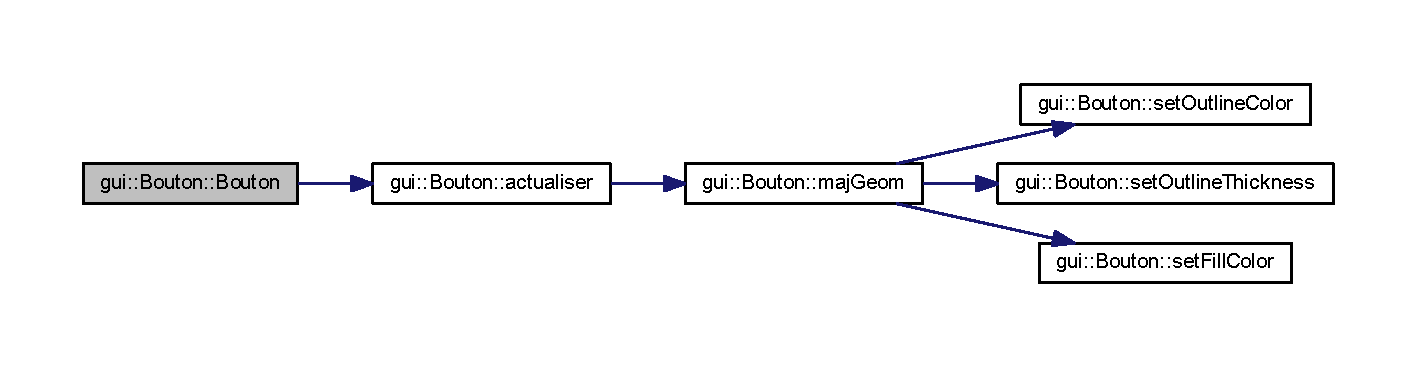
\includegraphics[width=350pt]{classgui_1_1_bouton_acb71294b84e82f435f81f272db595a3b_cgraph}
\end{center}
\end{figure}


\index{gui\+::\+Bouton@{gui\+::\+Bouton}!````~Bouton@{$\sim$\+Bouton}}
\index{````~Bouton@{$\sim$\+Bouton}!gui\+::\+Bouton@{gui\+::\+Bouton}}
\subsubsection[{$\sim$\+Bouton()}]{\setlength{\rightskip}{0pt plus 5cm}gui\+::\+Bouton\+::$\sim$\+Bouton (
\begin{DoxyParamCaption}
{}
\end{DoxyParamCaption}
)\hspace{0.3cm}{\ttfamily [virtual]}}\label{classgui_1_1_bouton_a7854d8a204c968aea377da67435bb50b}


Destructeur. 



\subsection{Documentation des fonctions membres}
\index{gui\+::\+Bouton@{gui\+::\+Bouton}!actualiser@{actualiser}}
\index{actualiser@{actualiser}!gui\+::\+Bouton@{gui\+::\+Bouton}}
\subsubsection[{actualiser(float delta\+T) override}]{\setlength{\rightskip}{0pt plus 5cm}void gui\+::\+Bouton\+::actualiser (
\begin{DoxyParamCaption}
\item[{float}]{delta\+T}
\end{DoxyParamCaption}
)\hspace{0.3cm}{\ttfamily [override]}, {\ttfamily [virtual]}}\label{classgui_1_1_bouton_a85874dc8b231bc9db24117aff6176d43}


Actualiser les éléments. 

Actualiser les différents éléments du ou des écrans actifs.


\begin{DoxyParams}{Paramètres}
{\em delta\+T} & Un {\itshape float} qui indique le delta du temps écoulé depuis la dernière actualisation. \\
\hline
\end{DoxyParams}
\begin{DoxyReturn}{Renvoie}
Rien 
\end{DoxyReturn}


Réimplémentée à partir de {\bf gui\+::\+Gadget} \doxyref{}{p.}{classgui_1_1_gadget_a06c66be095e4d531ef307a3db36e2b4f}.



Voici le graphe d\textquotesingle{}appel pour cette fonction \+:\nopagebreak
\begin{figure}[H]
\begin{center}
\leavevmode
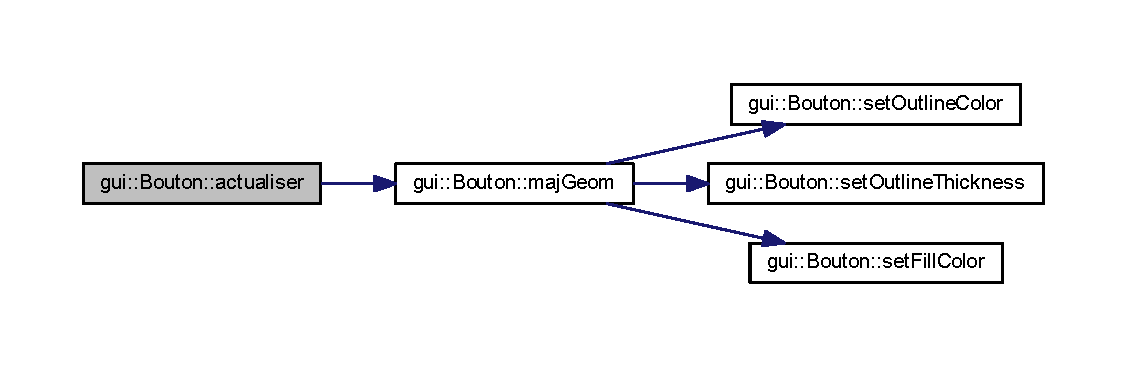
\includegraphics[width=350pt]{classgui_1_1_bouton_a85874dc8b231bc9db24117aff6176d43_cgraph}
\end{center}
\end{figure}




Voici le graphe des appelants de cette fonction \+:\nopagebreak
\begin{figure}[H]
\begin{center}
\leavevmode
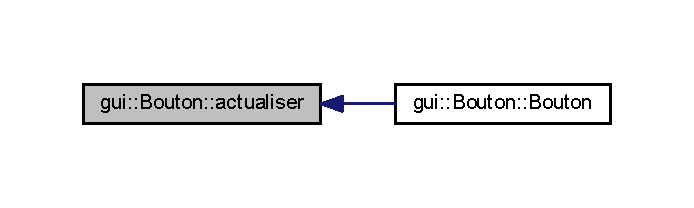
\includegraphics[width=333pt]{classgui_1_1_bouton_a85874dc8b231bc9db24117aff6176d43_icgraph}
\end{center}
\end{figure}


\index{gui\+::\+Bouton@{gui\+::\+Bouton}!draw@{draw}}
\index{draw@{draw}!gui\+::\+Bouton@{gui\+::\+Bouton}}
\subsubsection[{draw(sf\+::\+Render\+Target \&target, sf\+::\+Render\+States states) const }]{\setlength{\rightskip}{0pt plus 5cm}void gui\+::\+Bouton\+::draw (
\begin{DoxyParamCaption}
\item[{sf\+::\+Render\+Target \&}]{target, }
\item[{sf\+::\+Render\+States}]{states}
\end{DoxyParamCaption}
) const\hspace{0.3cm}{\ttfamily [virtual]}}\label{classgui_1_1_bouton_a8d736a0c912d7bb23551ccc0aaa0e20d}


Rendre les différents éléments du ou des écrans actifs. 



Réimplémentée à partir de {\bf gui\+::\+Gadget} \doxyref{}{p.}{classgui_1_1_gadget_a7ccb80ac58d4b1320bc76ad8ae031866}.



Réimplémentée dans {\bf gui\+::\+Bouton\+Texte} \doxyref{}{p.}{classgui_1_1_bouton_texte_ac07e5e027d4d9d3544e8964d5d370714}, et {\bf gui\+::\+Bouton\+Cocher} \doxyref{}{p.}{classgui_1_1_bouton_cocher_aea6c305290640a14a3659713b9acb5bf}.

\index{gui\+::\+Bouton@{gui\+::\+Bouton}!get\+Bordure@{get\+Bordure}}
\index{get\+Bordure@{get\+Bordure}!gui\+::\+Bouton@{gui\+::\+Bouton}}
\subsubsection[{get\+Bordure()}]{\setlength{\rightskip}{0pt plus 5cm}float gui\+::\+Bouton\+::get\+Bordure (
\begin{DoxyParamCaption}
{}
\end{DoxyParamCaption}
)\hspace{0.3cm}{\ttfamily [inline]}}\label{classgui_1_1_bouton_af4e656a92d7a1795a36d839ed9fa8501}


Acceder à la bordure du bouton. 

\begin{DoxyReturn}{Renvoie}
m\+\_\+bordure 
\end{DoxyReturn}
\index{gui\+::\+Bouton@{gui\+::\+Bouton}!get\+Global\+Bounds@{get\+Global\+Bounds}}
\index{get\+Global\+Bounds@{get\+Global\+Bounds}!gui\+::\+Bouton@{gui\+::\+Bouton}}
\subsubsection[{get\+Global\+Bounds()}]{\setlength{\rightskip}{0pt plus 5cm}sf\+::\+Float\+Rect gui\+::\+Bouton\+::get\+Global\+Bounds (
\begin{DoxyParamCaption}
{}
\end{DoxyParamCaption}
)\hspace{0.3cm}{\ttfamily [virtual]}}\label{classgui_1_1_bouton_a610e908477ecc3eef1576380ef5eda53}


Accesseur de la bounding\+Box en global. 

\begin{DoxyReturn}{Renvoie}
La bounding\+Box 
\end{DoxyReturn}


Réimplémentée à partir de {\bf gui\+::\+Gadget} \doxyref{}{p.}{classgui_1_1_gadget_a698682665f65f54e0798887955f32f2e}.



Voici le graphe d\textquotesingle{}appel pour cette fonction \+:\nopagebreak
\begin{figure}[H]
\begin{center}
\leavevmode
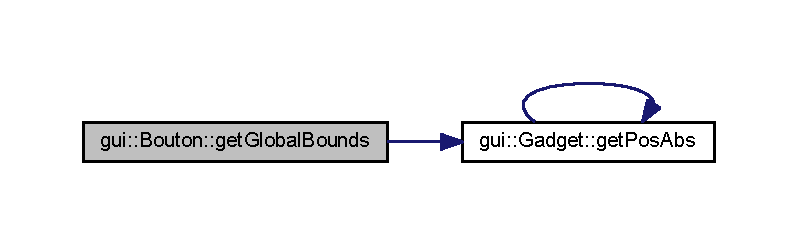
\includegraphics[width=350pt]{classgui_1_1_bouton_a610e908477ecc3eef1576380ef5eda53_cgraph}
\end{center}
\end{figure}


\index{gui\+::\+Bouton@{gui\+::\+Bouton}!get\+Local\+Bounds@{get\+Local\+Bounds}}
\index{get\+Local\+Bounds@{get\+Local\+Bounds}!gui\+::\+Bouton@{gui\+::\+Bouton}}
\subsubsection[{get\+Local\+Bounds()}]{\setlength{\rightskip}{0pt plus 5cm}sf\+::\+Float\+Rect gui\+::\+Bouton\+::get\+Local\+Bounds (
\begin{DoxyParamCaption}
{}
\end{DoxyParamCaption}
)\hspace{0.3cm}{\ttfamily [virtual]}}\label{classgui_1_1_bouton_a0f623480e174e03e1e23233dc991acea}


Accesseur de la bounding\+Box en local. 

\begin{DoxyReturn}{Renvoie}
La bounding\+Box 
\end{DoxyReturn}


Réimplémentée à partir de {\bf gui\+::\+Gadget} \doxyref{}{p.}{classgui_1_1_gadget_a4552567e63384c6a30519303f4052f11}.



Voici le graphe d\textquotesingle{}appel pour cette fonction \+:\nopagebreak
\begin{figure}[H]
\begin{center}
\leavevmode
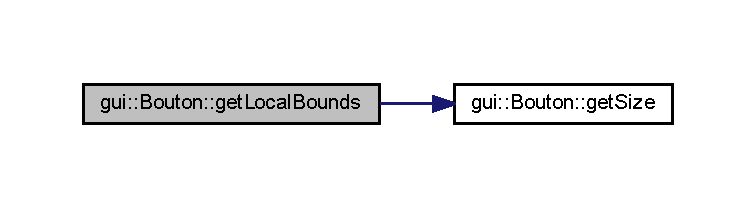
\includegraphics[width=350pt]{classgui_1_1_bouton_a0f623480e174e03e1e23233dc991acea_cgraph}
\end{center}
\end{figure}


\index{gui\+::\+Bouton@{gui\+::\+Bouton}!get\+Size@{get\+Size}}
\index{get\+Size@{get\+Size}!gui\+::\+Bouton@{gui\+::\+Bouton}}
\subsubsection[{get\+Size()}]{\setlength{\rightskip}{0pt plus 5cm}sf\+::\+Vector2f gui\+::\+Bouton\+::get\+Size (
\begin{DoxyParamCaption}
{}
\end{DoxyParamCaption}
)\hspace{0.3cm}{\ttfamily [virtual]}}\label{classgui_1_1_bouton_a971c98e0575c6b620454e399b91deb24}


Accesseur de la taille. 

\begin{DoxyReturn}{Renvoie}
La taille 
\end{DoxyReturn}


Réimplémentée à partir de {\bf gui\+::\+Gadget} \doxyref{}{p.}{classgui_1_1_gadget_a8d17e7736249da941358b9e09e70ea2c}.



Voici le graphe des appelants de cette fonction \+:\nopagebreak
\begin{figure}[H]
\begin{center}
\leavevmode
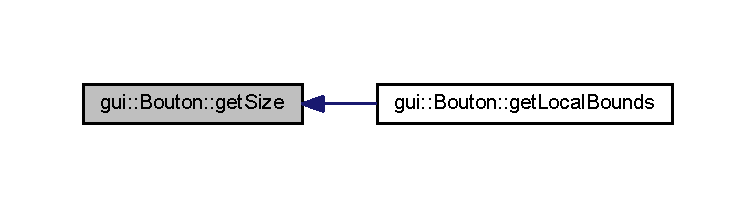
\includegraphics[width=350pt]{classgui_1_1_bouton_a971c98e0575c6b620454e399b91deb24_icgraph}
\end{center}
\end{figure}


\index{gui\+::\+Bouton@{gui\+::\+Bouton}!maj\+Geom@{maj\+Geom}}
\index{maj\+Geom@{maj\+Geom}!gui\+::\+Bouton@{gui\+::\+Bouton}}
\subsubsection[{maj\+Geom()}]{\setlength{\rightskip}{0pt plus 5cm}void gui\+::\+Bouton\+::maj\+Geom (
\begin{DoxyParamCaption}
{}
\end{DoxyParamCaption}
)\hspace{0.3cm}{\ttfamily [protected]}, {\ttfamily [virtual]}}\label{classgui_1_1_bouton_a1ff3d7a1586eaab5873cc6e49be2332c}


Actualise le style du label. 

\begin{DoxyReturn}{Renvoie}
Rien 
\end{DoxyReturn}


Réimplémentée à partir de {\bf gui\+::\+Gadget} \doxyref{}{p.}{classgui_1_1_gadget_a8a72d0816ec1928958ff5dd3ccd983f5}.



Réimplémentée dans {\bf gui\+::\+Bouton\+Texte} \doxyref{}{p.}{classgui_1_1_bouton_texte_a6c66a5e34585fdb6054c2f56160db0a7}, et {\bf gui\+::\+Bouton\+Cocher} \doxyref{}{p.}{classgui_1_1_bouton_cocher_a03a7011fd1269a5502fd3b6e58652c4e}.



Voici le graphe d\textquotesingle{}appel pour cette fonction \+:\nopagebreak
\begin{figure}[H]
\begin{center}
\leavevmode
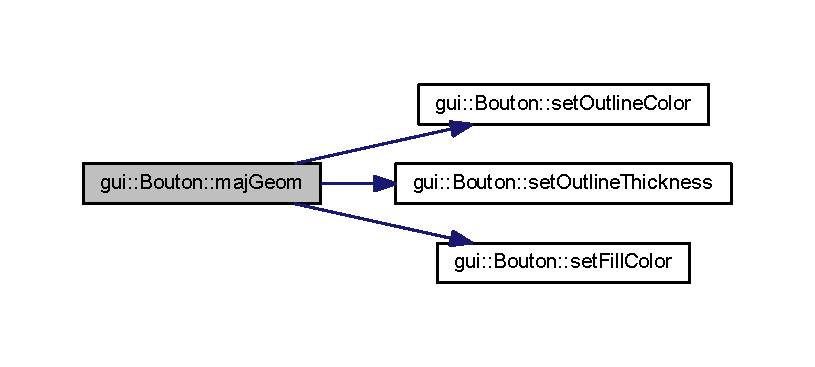
\includegraphics[width=350pt]{classgui_1_1_bouton_a1ff3d7a1586eaab5873cc6e49be2332c_cgraph}
\end{center}
\end{figure}




Voici le graphe des appelants de cette fonction \+:\nopagebreak
\begin{figure}[H]
\begin{center}
\leavevmode
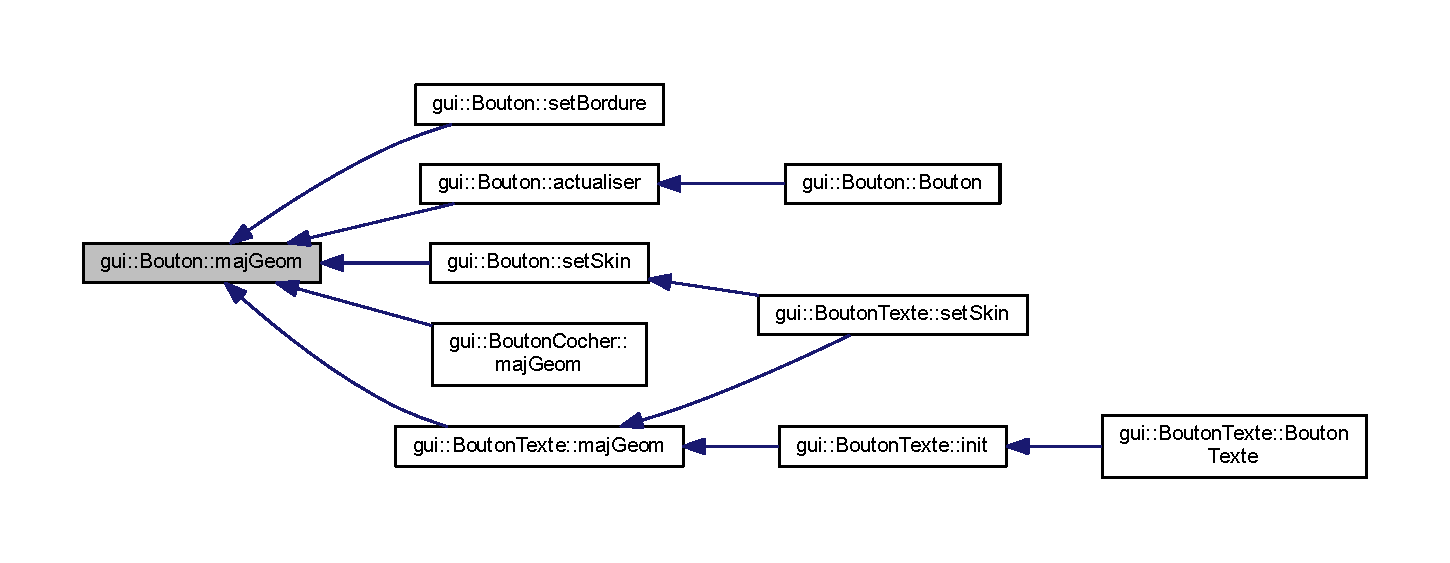
\includegraphics[width=350pt]{classgui_1_1_bouton_a1ff3d7a1586eaab5873cc6e49be2332c_icgraph}
\end{center}
\end{figure}


\index{gui\+::\+Bouton@{gui\+::\+Bouton}!set\+Bordure@{set\+Bordure}}
\index{set\+Bordure@{set\+Bordure}!gui\+::\+Bouton@{gui\+::\+Bouton}}
\subsubsection[{set\+Bordure(float val)}]{\setlength{\rightskip}{0pt plus 5cm}void gui\+::\+Bouton\+::set\+Bordure (
\begin{DoxyParamCaption}
\item[{float}]{val}
\end{DoxyParamCaption}
)\hspace{0.3cm}{\ttfamily [inline]}}\label{classgui_1_1_bouton_a64b944ce671d491c2c14087b5727ee0b}


Definir la bordure du texte. 


\begin{DoxyParams}{Paramètres}
{\em val} & la nouvelle valeur pour la bordure m\+\_\+bordure. \\
\hline
\end{DoxyParams}


Voici le graphe d\textquotesingle{}appel pour cette fonction \+:\nopagebreak
\begin{figure}[H]
\begin{center}
\leavevmode
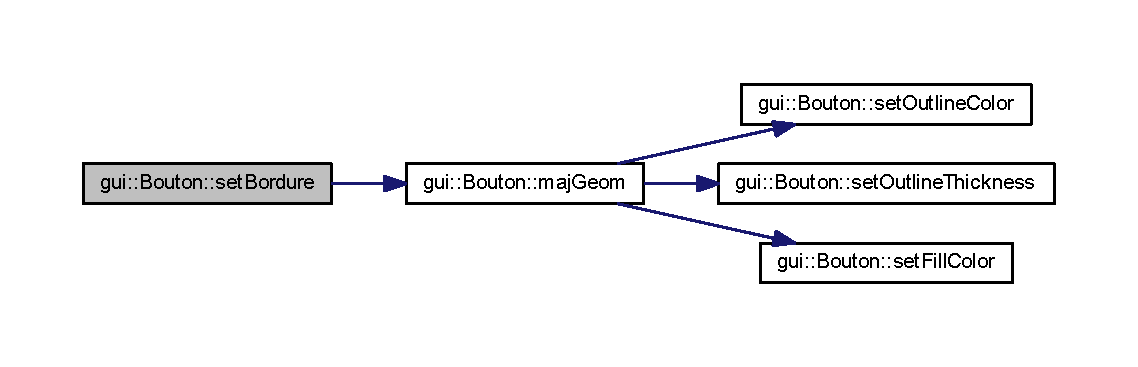
\includegraphics[width=350pt]{classgui_1_1_bouton_a64b944ce671d491c2c14087b5727ee0b_cgraph}
\end{center}
\end{figure}


\index{gui\+::\+Bouton@{gui\+::\+Bouton}!set\+Fill\+Color@{set\+Fill\+Color}}
\index{set\+Fill\+Color@{set\+Fill\+Color}!gui\+::\+Bouton@{gui\+::\+Bouton}}
\subsubsection[{set\+Fill\+Color(sf\+::\+Color color)}]{\setlength{\rightskip}{0pt plus 5cm}void gui\+::\+Bouton\+::set\+Fill\+Color (
\begin{DoxyParamCaption}
\item[{sf\+::\+Color}]{color}
\end{DoxyParamCaption}
)\hspace{0.3cm}{\ttfamily [virtual]}}\label{classgui_1_1_bouton_a84b817726afad13e2c93b458df712beb}


Definir Couleur du fond. 


\begin{DoxyParams}{Paramètres}
{\em color} & La nouvelle Couleur du fond. \\
\hline
\end{DoxyParams}
\begin{DoxyReturn}{Renvoie}
Rien 
\end{DoxyReturn}


Voici le graphe des appelants de cette fonction \+:\nopagebreak
\begin{figure}[H]
\begin{center}
\leavevmode
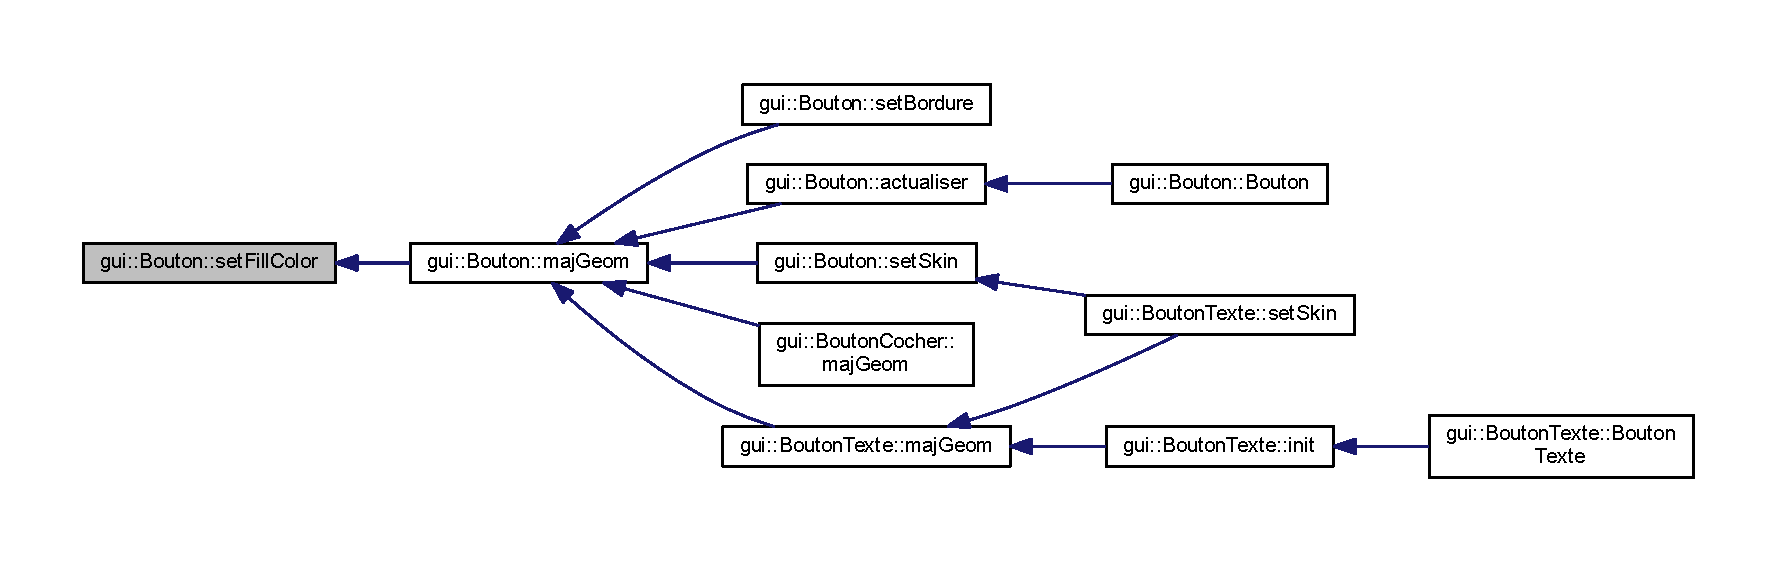
\includegraphics[width=350pt]{classgui_1_1_bouton_a84b817726afad13e2c93b458df712beb_icgraph}
\end{center}
\end{figure}


\index{gui\+::\+Bouton@{gui\+::\+Bouton}!set\+Outline\+Color@{set\+Outline\+Color}}
\index{set\+Outline\+Color@{set\+Outline\+Color}!gui\+::\+Bouton@{gui\+::\+Bouton}}
\subsubsection[{set\+Outline\+Color(sf\+::\+Color color)}]{\setlength{\rightskip}{0pt plus 5cm}void gui\+::\+Bouton\+::set\+Outline\+Color (
\begin{DoxyParamCaption}
\item[{sf\+::\+Color}]{color}
\end{DoxyParamCaption}
)\hspace{0.3cm}{\ttfamily [virtual]}}\label{classgui_1_1_bouton_a82ae2f53840fa81e95bad972a301bddb}


Definir Couleur du cadre. 


\begin{DoxyParams}{Paramètres}
{\em color} & La nouvelle Couleur du cadre. \\
\hline
\end{DoxyParams}
\begin{DoxyReturn}{Renvoie}
Rien 
\end{DoxyReturn}


Voici le graphe des appelants de cette fonction \+:\nopagebreak
\begin{figure}[H]
\begin{center}
\leavevmode
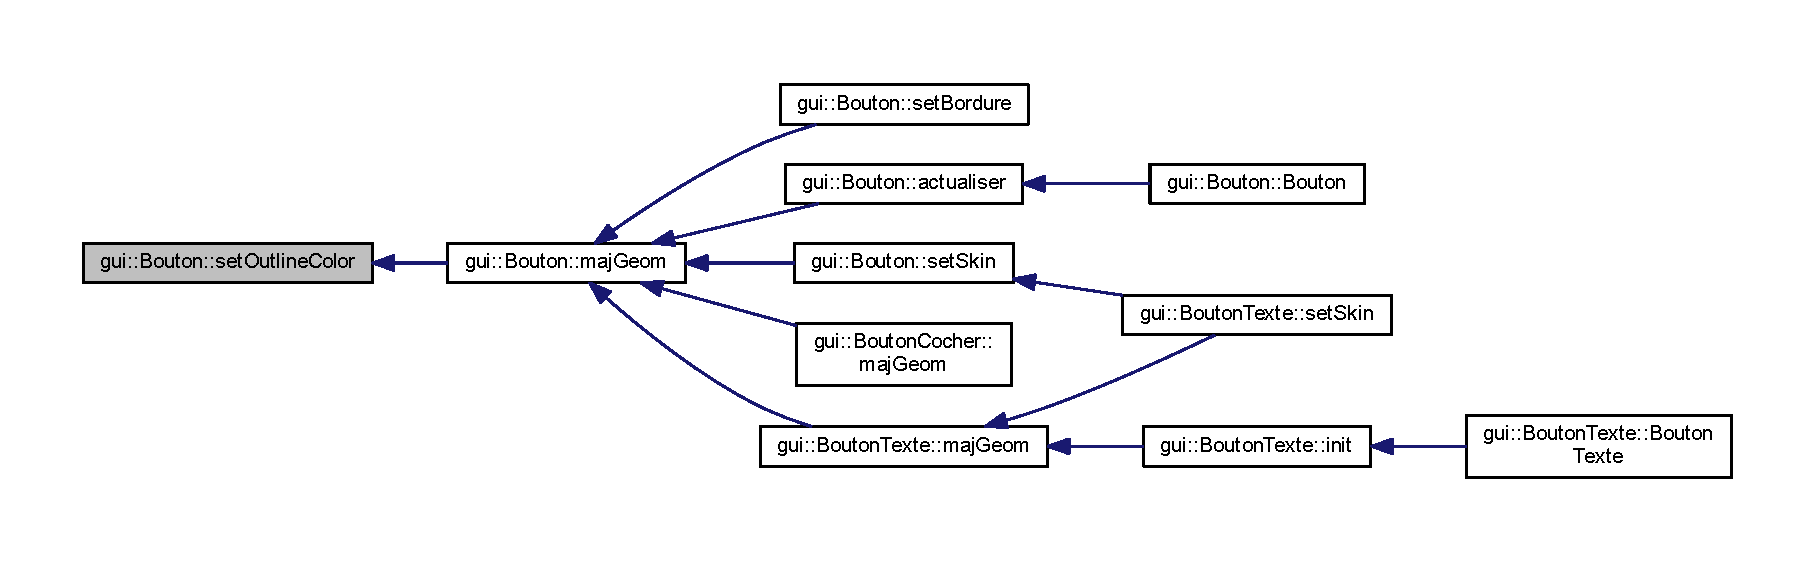
\includegraphics[width=350pt]{classgui_1_1_bouton_a82ae2f53840fa81e95bad972a301bddb_icgraph}
\end{center}
\end{figure}


\index{gui\+::\+Bouton@{gui\+::\+Bouton}!set\+Outline\+Thickness@{set\+Outline\+Thickness}}
\index{set\+Outline\+Thickness@{set\+Outline\+Thickness}!gui\+::\+Bouton@{gui\+::\+Bouton}}
\subsubsection[{set\+Outline\+Thickness(float epaisseur)}]{\setlength{\rightskip}{0pt plus 5cm}void gui\+::\+Bouton\+::set\+Outline\+Thickness (
\begin{DoxyParamCaption}
\item[{float}]{epaisseur}
\end{DoxyParamCaption}
)\hspace{0.3cm}{\ttfamily [virtual]}}\label{classgui_1_1_bouton_ae56f585c1463d258f7209ade57426421}


Definir l\textquotesingle{}épaisseur du cadre. 


\begin{DoxyParams}{Paramètres}
{\em epaisseur} & La nouvelle épaisseur du cadre. \\
\hline
\end{DoxyParams}
\begin{DoxyReturn}{Renvoie}
Rien 
\end{DoxyReturn}


Voici le graphe des appelants de cette fonction \+:\nopagebreak
\begin{figure}[H]
\begin{center}
\leavevmode
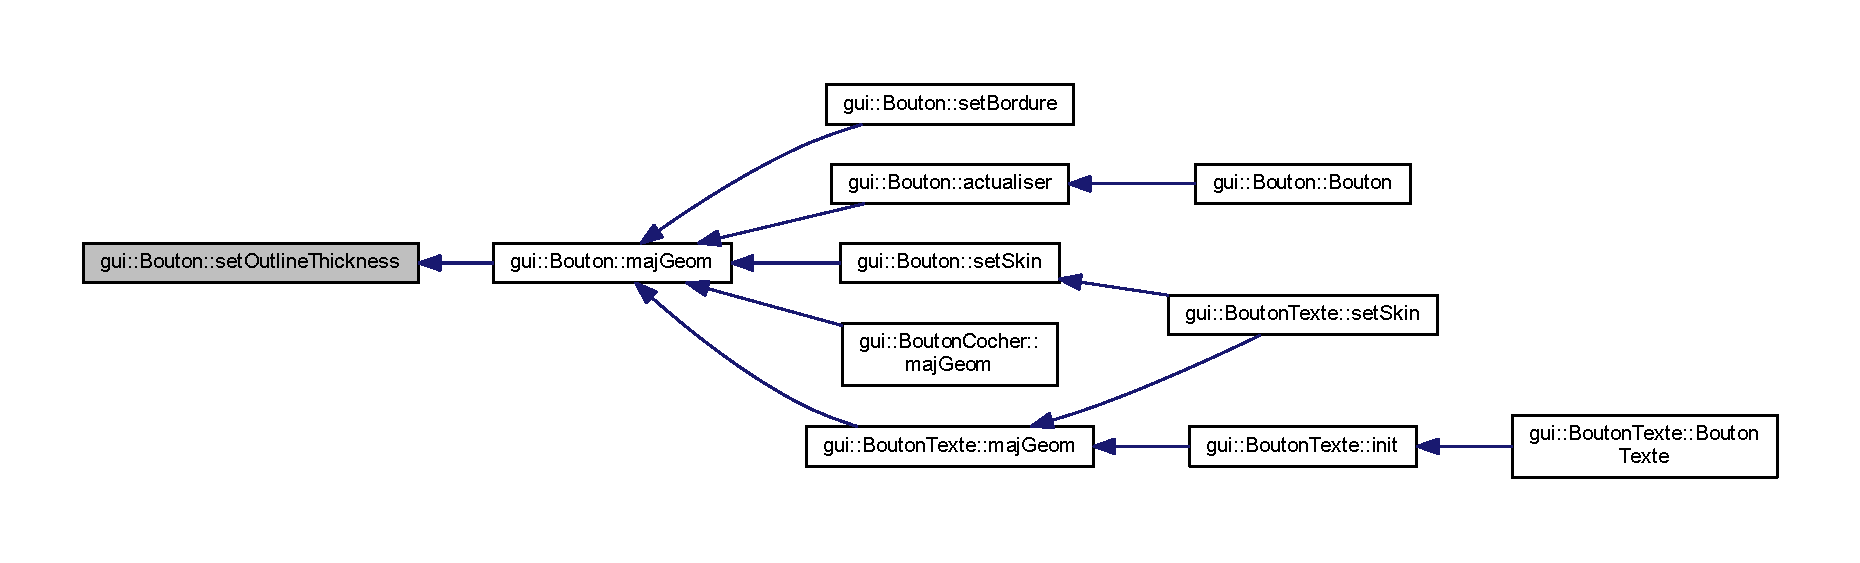
\includegraphics[width=350pt]{classgui_1_1_bouton_ae56f585c1463d258f7209ade57426421_icgraph}
\end{center}
\end{figure}


\index{gui\+::\+Bouton@{gui\+::\+Bouton}!set\+Size@{set\+Size}}
\index{set\+Size@{set\+Size}!gui\+::\+Bouton@{gui\+::\+Bouton}}
\subsubsection[{set\+Size(sf\+::\+Vector2f taille)}]{\setlength{\rightskip}{0pt plus 5cm}void gui\+::\+Bouton\+::set\+Size (
\begin{DoxyParamCaption}
\item[{sf\+::\+Vector2f}]{taille}
\end{DoxyParamCaption}
)\hspace{0.3cm}{\ttfamily [virtual]}}\label{classgui_1_1_bouton_a7652dfbbb1180cfecc0db6b68db38776}


Definir la taille du bouton. 


\begin{DoxyParams}{Paramètres}
{\em taille} & La nouvelle taille. \\
\hline
\end{DoxyParams}
\begin{DoxyReturn}{Renvoie}
Rien 
\end{DoxyReturn}


Réimplémentée à partir de {\bf gui\+::\+Gadget} \doxyref{}{p.}{classgui_1_1_gadget_a2d021f2ce19a4335d79bcaedf4ab4bb2}.



Réimplémentée dans {\bf gui\+::\+Bouton\+Texte} \doxyref{}{p.}{classgui_1_1_bouton_texte_a1725dffd7f645561ee4db8786d83a85e}.

\index{gui\+::\+Bouton@{gui\+::\+Bouton}!set\+Skin@{set\+Skin}}
\index{set\+Skin@{set\+Skin}!gui\+::\+Bouton@{gui\+::\+Bouton}}
\subsubsection[{set\+Skin(std\+::shared\+\_\+ptr$<$ Skin $>$ skin)}]{\setlength{\rightskip}{0pt plus 5cm}void gui\+::\+Bouton\+::set\+Skin (
\begin{DoxyParamCaption}
\item[{std\+::shared\+\_\+ptr$<$ {\bf Skin} $>$}]{skin}
\end{DoxyParamCaption}
)\hspace{0.3cm}{\ttfamily [virtual]}}\label{classgui_1_1_bouton_aba971350f784988e1a03328264e551bb}


Définie le skin du \doxyref{Label}{p.}{classgui_1_1_label}. 


\begin{DoxyParams}{Paramètres}
{\em skin} & Le skin à appliquer (Configuration\+::\+Styles).\\
\hline
\end{DoxyParams}
return Rien 

Réimplémentée à partir de {\bf gui\+::\+Gadget} \doxyref{}{p.}{classgui_1_1_gadget_a93ede42252a94de3b756a9a5761df3a7}.



Réimplémentée dans {\bf gui\+::\+Bouton\+Texte} \doxyref{}{p.}{classgui_1_1_bouton_texte_ab8059cd7c83e678dd8b3c9dba62a2363}.



Voici le graphe d\textquotesingle{}appel pour cette fonction \+:\nopagebreak
\begin{figure}[H]
\begin{center}
\leavevmode
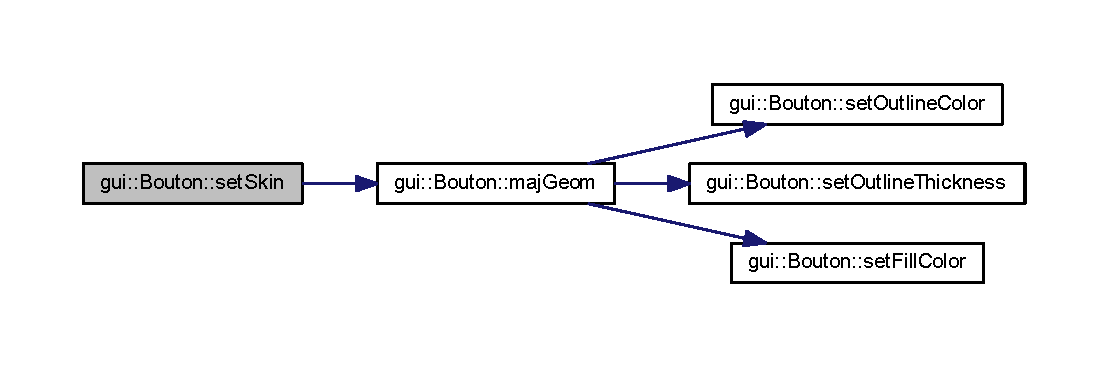
\includegraphics[width=350pt]{classgui_1_1_bouton_aba971350f784988e1a03328264e551bb_cgraph}
\end{center}
\end{figure}




Voici le graphe des appelants de cette fonction \+:\nopagebreak
\begin{figure}[H]
\begin{center}
\leavevmode
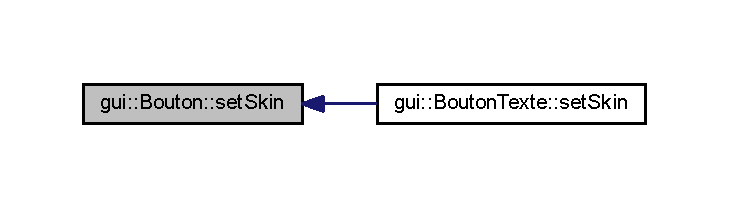
\includegraphics[width=350pt]{classgui_1_1_bouton_aba971350f784988e1a03328264e551bb_icgraph}
\end{center}
\end{figure}


\index{gui\+::\+Bouton@{gui\+::\+Bouton}!traiter\+\_\+evenements@{traiter\+\_\+evenements}}
\index{traiter\+\_\+evenements@{traiter\+\_\+evenements}!gui\+::\+Bouton@{gui\+::\+Bouton}}
\subsubsection[{traiter\+\_\+evenements(const sf\+::\+Event \&event)}]{\setlength{\rightskip}{0pt plus 5cm}void gui\+::\+Bouton\+::traiter\+\_\+evenements (
\begin{DoxyParamCaption}
\item[{const sf\+::\+Event \&}]{event}
\end{DoxyParamCaption}
)\hspace{0.3cm}{\ttfamily [virtual]}}\label{classgui_1_1_bouton_a86f25f637d31c49cbc128bbeb62b01ac}


La gestion des évènements utilisateurs. 

Gère les entrées claviers, souris, fenetre ...


\begin{DoxyParams}{Paramètres}
{\em event} & evenement S\+F\+M\+L se transmettant depuis l\textquotesingle{}application \\
\hline
\end{DoxyParams}
\begin{DoxyReturn}{Renvoie}
Rien 
\end{DoxyReturn}


Réimplémentée à partir de {\bf gui\+::\+Gadget} \doxyref{}{p.}{classgui_1_1_gadget_a510ae68144997724188d2bb902c3103d}.



Voici le graphe d\textquotesingle{}appel pour cette fonction \+:\nopagebreak
\begin{figure}[H]
\begin{center}
\leavevmode
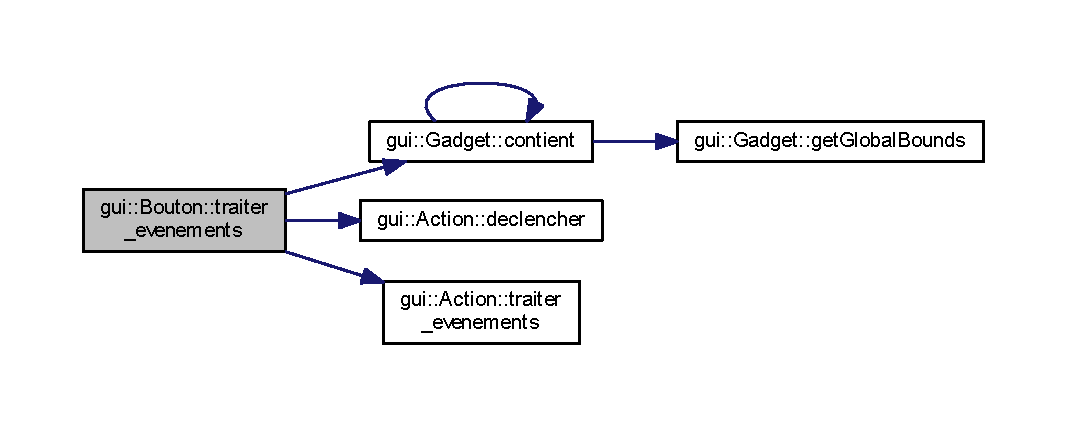
\includegraphics[width=350pt]{classgui_1_1_bouton_a86f25f637d31c49cbc128bbeb62b01ac_cgraph}
\end{center}
\end{figure}




\subsection{Documentation des champs}
\index{gui\+::\+Bouton@{gui\+::\+Bouton}!m\+\_\+1er\+Click@{m\+\_\+1er\+Click}}
\index{m\+\_\+1er\+Click@{m\+\_\+1er\+Click}!gui\+::\+Bouton@{gui\+::\+Bouton}}
\subsubsection[{m\+\_\+1er\+Click}]{\setlength{\rightskip}{0pt plus 5cm}bool gui\+::\+Bouton\+::m\+\_\+1er\+Click\hspace{0.3cm}{\ttfamily [protected]}}\label{classgui_1_1_bouton_aed2b58479b336c984960936f3ce33caa}


bool double clique, true lors du 1er clique, false a la fin du temps ou apres second clique. 

\index{gui\+::\+Bouton@{gui\+::\+Bouton}!m\+\_\+bordure@{m\+\_\+bordure}}
\index{m\+\_\+bordure@{m\+\_\+bordure}!gui\+::\+Bouton@{gui\+::\+Bouton}}
\subsubsection[{m\+\_\+bordure}]{\setlength{\rightskip}{0pt plus 5cm}float gui\+::\+Bouton\+::m\+\_\+bordure\hspace{0.3cm}{\ttfamily [protected]}}\label{classgui_1_1_bouton_a66fd43d3a26b7c86f43990d94217d5a1}


l\textquotesingle{}espace de bordure (pour gui\+::bouton\+Texte, gui\+::\+Bouton\+Coher ..). 

\index{gui\+::\+Bouton@{gui\+::\+Bouton}!m\+\_\+clock\+\_\+dbl\+Clique@{m\+\_\+clock\+\_\+dbl\+Clique}}
\index{m\+\_\+clock\+\_\+dbl\+Clique@{m\+\_\+clock\+\_\+dbl\+Clique}!gui\+::\+Bouton@{gui\+::\+Bouton}}
\subsubsection[{m\+\_\+clock\+\_\+dbl\+Clique}]{\setlength{\rightskip}{0pt plus 5cm}sf\+::\+Clock gui\+::\+Bouton\+::m\+\_\+clock\+\_\+dbl\+Clique\hspace{0.3cm}{\ttfamily [protected]}}\label{classgui_1_1_bouton_aa16f60426d96ef6d73a7e436d5a31027}


Compteur temps pour double clique. 

\index{gui\+::\+Bouton@{gui\+::\+Bouton}!m\+\_\+etat@{m\+\_\+etat}}
\index{m\+\_\+etat@{m\+\_\+etat}!gui\+::\+Bouton@{gui\+::\+Bouton}}
\subsubsection[{m\+\_\+etat}]{\setlength{\rightskip}{0pt plus 5cm}{\bf Etat\+Bouton} gui\+::\+Bouton\+::m\+\_\+etat\hspace{0.3cm}{\ttfamily [protected]}}\label{classgui_1_1_bouton_a92ed42af744e499c3d94b0911589761f}


L\textquotesingle{}état du bouton. 

\index{gui\+::\+Bouton@{gui\+::\+Bouton}!m\+\_\+etat\+Back@{m\+\_\+etat\+Back}}
\index{m\+\_\+etat\+Back@{m\+\_\+etat\+Back}!gui\+::\+Bouton@{gui\+::\+Bouton}}
\subsubsection[{m\+\_\+etat\+Back}]{\setlength{\rightskip}{0pt plus 5cm}{\bf Etat\+Bouton} gui\+::\+Bouton\+::m\+\_\+etat\+Back\hspace{0.3cm}{\ttfamily [protected]}}\label{classgui_1_1_bouton_a8f8714ab82973e57eb3ee4f85c4a324b}


L\textquotesingle{}état du bouton la frame d\textquotesingle{}avant, pour verifier si changement d\textquotesingle{}état. 

\index{gui\+::\+Bouton@{gui\+::\+Bouton}!m\+\_\+fond@{m\+\_\+fond}}
\index{m\+\_\+fond@{m\+\_\+fond}!gui\+::\+Bouton@{gui\+::\+Bouton}}
\subsubsection[{m\+\_\+fond}]{\setlength{\rightskip}{0pt plus 5cm}std\+::shared\+\_\+ptr$<${\bf Image}$>$ gui\+::\+Bouton\+::m\+\_\+fond\hspace{0.3cm}{\ttfamily [protected]}}\label{classgui_1_1_bouton_a8a9c0b300e1af08d60200f29fc503031}


Le rectangle du fond du bouton. 



La documentation de cette classe a été générée à partir des fichiers suivants \+:\begin{DoxyCompactItemize}
\item 
Interface/include/gadgets/{\bf Bouton.\+h}\item 
Interface/src/gadgets/{\bf Bouton.\+cpp}\end{DoxyCompactItemize}

\section{Référence de la classe gui\+:\+:Bouton\+Cocher}
\label{classgui_1_1_bouton_cocher}\index{gui\+::\+Bouton\+Cocher@{gui\+::\+Bouton\+Cocher}}


\doxyref{Gadget}{p.}{classgui_1_1_gadget}, bouton rectangulaire à cocher,.  




{\ttfamily \#include $<$Bouton\+Cocher.\+h$>$}



Graphe d\textquotesingle{}héritage de gui\+:\+:Bouton\+Cocher\+:\nopagebreak
\begin{figure}[H]
\begin{center}
\leavevmode
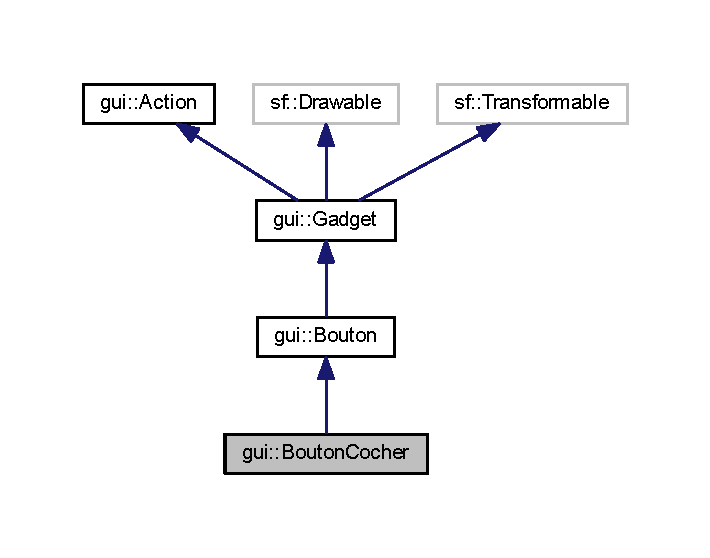
\includegraphics[width=341pt]{classgui_1_1_bouton_cocher__inherit__graph}
\end{center}
\end{figure}


Graphe de collaboration de gui\+:\+:Bouton\+Cocher\+:\nopagebreak
\begin{figure}[H]
\begin{center}
\leavevmode
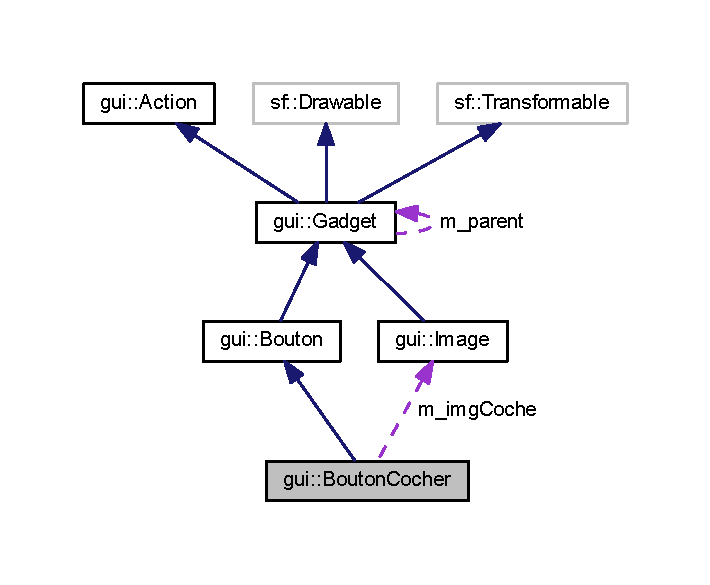
\includegraphics[width=341pt]{classgui_1_1_bouton_cocher__coll__graph}
\end{center}
\end{figure}
\subsection*{Fonctions membres publiques}
\begin{DoxyCompactItemize}
\item 
{\bf Bouton\+Cocher} ()
\begin{DoxyCompactList}\small\item\em Constructeur. \end{DoxyCompactList}\item 
{\bf Bouton\+Cocher} (std\+::shared\+\_\+ptr$<$ {\bf Skin} $>$ skin, bool actif=false)
\begin{DoxyCompactList}\small\item\em Constructeur avec definition du skin et valeur de l\textquotesingle{}état du bouton. \end{DoxyCompactList}\item 
virtual {\bf $\sim$\+Bouton\+Cocher} ()
\begin{DoxyCompactList}\small\item\em Destructeur. \end{DoxyCompactList}\item 
void {\bf set\+Actif} (bool actif)
\begin{DoxyCompactList}\small\item\em Définir l\textquotesingle{}état du bouton. \end{DoxyCompactList}\item 
bool {\bf is\+Actif} ()
\begin{DoxyCompactList}\small\item\em demande l\textquotesingle{}état du bouton \end{DoxyCompactList}\item 
virtual void {\bf maj\+Geom} ()
\begin{DoxyCompactList}\small\item\em Actualise le model du \doxyref{Gadget}{p.}{classgui_1_1_gadget}. \end{DoxyCompactList}\item 
virtual void {\bf draw} (sf\+::\+Render\+Target \&target, sf\+::\+Render\+States states) const 
\begin{DoxyCompactList}\small\item\em Rendre les différents éléments du ou des écrans actifs. \end{DoxyCompactList}\end{DoxyCompactItemize}
\subsection*{Fonctions membres privées}
\begin{DoxyCompactItemize}
\item 
virtual void {\bf init} ()
\begin{DoxyCompactList}\small\item\em initialisation du gadget. \end{DoxyCompactList}\end{DoxyCompactItemize}
\subsection*{Attributs privés}
\begin{DoxyCompactItemize}
\item 
bool {\bf m\+\_\+actif}
\begin{DoxyCompactList}\small\item\em l\textquotesingle{}état du bouton (true\+: coché ou false\+:décoché). \end{DoxyCompactList}\item 
{\bf Image} $\ast$ {\bf m\+\_\+img\+Coche}
\begin{DoxyCompactList}\small\item\em le gadget \doxyref{Image}{p.}{classgui_1_1_image} qui est visible si le bouton est coché. \end{DoxyCompactList}\item 
{\bf Func\+Type} {\bf m\+\_\+fct\+Toggle}
\begin{DoxyCompactList}\small\item\em la fonction qui change l\textquotesingle{}état du bouton a chaque clique. \end{DoxyCompactList}\end{DoxyCompactItemize}
\subsection*{Membres hérités additionnels}


\subsection{Description détaillée}
\doxyref{Gadget}{p.}{classgui_1_1_gadget}, bouton rectangulaire à cocher,. 

\begin{DoxySeeAlso}{Voir également}
\doxyref{gui\+::\+Gadget}{p.}{classgui_1_1_gadget} 
\end{DoxySeeAlso}


\subsection{Documentation des constructeurs et destructeur}
\index{gui\+::\+Bouton\+Cocher@{gui\+::\+Bouton\+Cocher}!Bouton\+Cocher@{Bouton\+Cocher}}
\index{Bouton\+Cocher@{Bouton\+Cocher}!gui\+::\+Bouton\+Cocher@{gui\+::\+Bouton\+Cocher}}
\subsubsection[{Bouton\+Cocher()}]{\setlength{\rightskip}{0pt plus 5cm}gui\+::\+Bouton\+Cocher\+::\+Bouton\+Cocher (
\begin{DoxyParamCaption}
{}
\end{DoxyParamCaption}
)}\label{classgui_1_1_bouton_cocher_a7b5e763ff726740b19ec6758e6431b92}


Constructeur. 



Voici le graphe d\textquotesingle{}appel pour cette fonction \+:\nopagebreak
\begin{figure}[H]
\begin{center}
\leavevmode
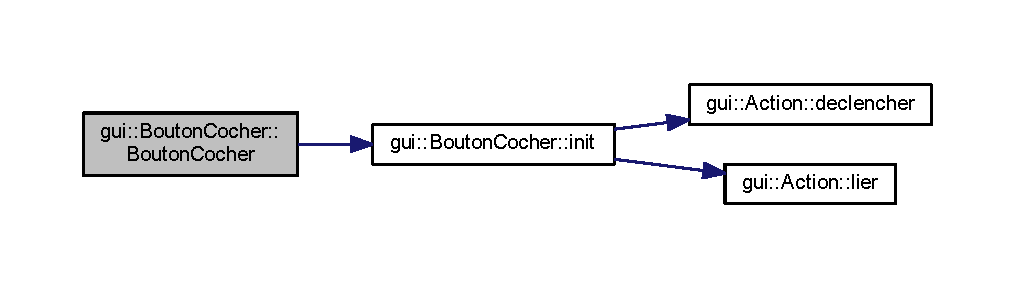
\includegraphics[width=350pt]{classgui_1_1_bouton_cocher_a7b5e763ff726740b19ec6758e6431b92_cgraph}
\end{center}
\end{figure}


\index{gui\+::\+Bouton\+Cocher@{gui\+::\+Bouton\+Cocher}!Bouton\+Cocher@{Bouton\+Cocher}}
\index{Bouton\+Cocher@{Bouton\+Cocher}!gui\+::\+Bouton\+Cocher@{gui\+::\+Bouton\+Cocher}}
\subsubsection[{Bouton\+Cocher(std\+::shared\+\_\+ptr$<$ Skin $>$ skin, bool actif=false)}]{\setlength{\rightskip}{0pt plus 5cm}gui\+::\+Bouton\+Cocher\+::\+Bouton\+Cocher (
\begin{DoxyParamCaption}
\item[{std\+::shared\+\_\+ptr$<$ {\bf Skin} $>$}]{skin, }
\item[{bool}]{actif = {\ttfamily false}}
\end{DoxyParamCaption}
)}\label{classgui_1_1_bouton_cocher_ac6d72b56515735de4121a2623c3c1a17}


Constructeur avec definition du skin et valeur de l\textquotesingle{}état du bouton. 


\begin{DoxyParams}{Paramètres}
{\em skin} & les skin à utiliser pour ce bouton. \\
\hline
{\em actif} & l\textquotesingle{}état du bouton. \\
\hline
\end{DoxyParams}


Voici le graphe d\textquotesingle{}appel pour cette fonction \+:\nopagebreak
\begin{figure}[H]
\begin{center}
\leavevmode
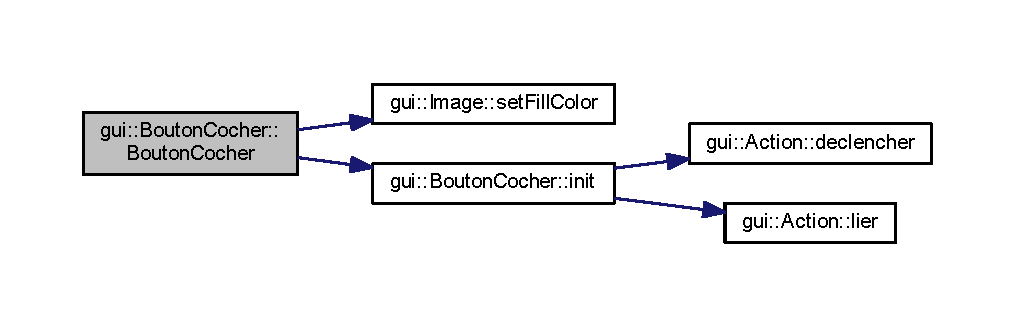
\includegraphics[width=350pt]{classgui_1_1_bouton_cocher_ac6d72b56515735de4121a2623c3c1a17_cgraph}
\end{center}
\end{figure}


\index{gui\+::\+Bouton\+Cocher@{gui\+::\+Bouton\+Cocher}!````~Bouton\+Cocher@{$\sim$\+Bouton\+Cocher}}
\index{````~Bouton\+Cocher@{$\sim$\+Bouton\+Cocher}!gui\+::\+Bouton\+Cocher@{gui\+::\+Bouton\+Cocher}}
\subsubsection[{$\sim$\+Bouton\+Cocher()}]{\setlength{\rightskip}{0pt plus 5cm}gui\+::\+Bouton\+Cocher\+::$\sim$\+Bouton\+Cocher (
\begin{DoxyParamCaption}
{}
\end{DoxyParamCaption}
)\hspace{0.3cm}{\ttfamily [virtual]}}\label{classgui_1_1_bouton_cocher_a47881be4183b985ba8957ed7f3219d7e}


Destructeur. 



\subsection{Documentation des fonctions membres}
\index{gui\+::\+Bouton\+Cocher@{gui\+::\+Bouton\+Cocher}!draw@{draw}}
\index{draw@{draw}!gui\+::\+Bouton\+Cocher@{gui\+::\+Bouton\+Cocher}}
\subsubsection[{draw(sf\+::\+Render\+Target \&target, sf\+::\+Render\+States states) const }]{\setlength{\rightskip}{0pt plus 5cm}void gui\+::\+Bouton\+Cocher\+::draw (
\begin{DoxyParamCaption}
\item[{sf\+::\+Render\+Target \&}]{target, }
\item[{sf\+::\+Render\+States}]{states}
\end{DoxyParamCaption}
) const\hspace{0.3cm}{\ttfamily [virtual]}}\label{classgui_1_1_bouton_cocher_aea6c305290640a14a3659713b9acb5bf}


Rendre les différents éléments du ou des écrans actifs. 



Réimplémentée à partir de {\bf gui\+::\+Bouton} \doxyref{}{p.}{classgui_1_1_bouton_a8d736a0c912d7bb23551ccc0aaa0e20d}.

\index{gui\+::\+Bouton\+Cocher@{gui\+::\+Bouton\+Cocher}!init@{init}}
\index{init@{init}!gui\+::\+Bouton\+Cocher@{gui\+::\+Bouton\+Cocher}}
\subsubsection[{init()}]{\setlength{\rightskip}{0pt plus 5cm}void gui\+::\+Bouton\+Cocher\+::init (
\begin{DoxyParamCaption}
{}
\end{DoxyParamCaption}
)\hspace{0.3cm}{\ttfamily [private]}, {\ttfamily [virtual]}}\label{classgui_1_1_bouton_cocher_a92470d7fc9202d991e8499331660ba8c}


initialisation du gadget. 

\begin{DoxyReturn}{Renvoie}
Rien 
\end{DoxyReturn}


Voici le graphe d\textquotesingle{}appel pour cette fonction \+:\nopagebreak
\begin{figure}[H]
\begin{center}
\leavevmode
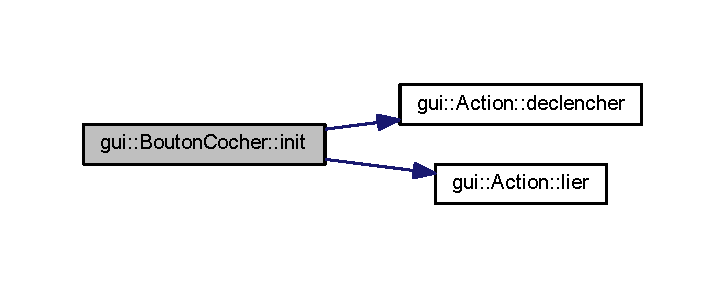
\includegraphics[width=348pt]{classgui_1_1_bouton_cocher_a92470d7fc9202d991e8499331660ba8c_cgraph}
\end{center}
\end{figure}




Voici le graphe des appelants de cette fonction \+:\nopagebreak
\begin{figure}[H]
\begin{center}
\leavevmode
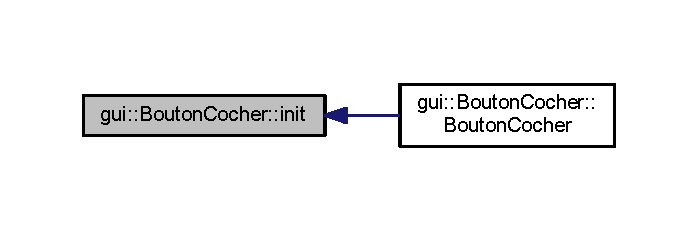
\includegraphics[width=335pt]{classgui_1_1_bouton_cocher_a92470d7fc9202d991e8499331660ba8c_icgraph}
\end{center}
\end{figure}


\index{gui\+::\+Bouton\+Cocher@{gui\+::\+Bouton\+Cocher}!is\+Actif@{is\+Actif}}
\index{is\+Actif@{is\+Actif}!gui\+::\+Bouton\+Cocher@{gui\+::\+Bouton\+Cocher}}
\subsubsection[{is\+Actif()}]{\setlength{\rightskip}{0pt plus 5cm}bool gui\+::\+Bouton\+Cocher\+::is\+Actif (
\begin{DoxyParamCaption}
{}
\end{DoxyParamCaption}
)\hspace{0.3cm}{\ttfamily [inline]}}\label{classgui_1_1_bouton_cocher_a1bfe8ca9d1f45890f594ff392227fa28}


demande l\textquotesingle{}état du bouton 

\begin{DoxyReturn}{Renvoie}
true \+: coché, false \+: décoché. 
\end{DoxyReturn}
\index{gui\+::\+Bouton\+Cocher@{gui\+::\+Bouton\+Cocher}!maj\+Geom@{maj\+Geom}}
\index{maj\+Geom@{maj\+Geom}!gui\+::\+Bouton\+Cocher@{gui\+::\+Bouton\+Cocher}}
\subsubsection[{maj\+Geom()}]{\setlength{\rightskip}{0pt plus 5cm}void gui\+::\+Bouton\+Cocher\+::maj\+Geom (
\begin{DoxyParamCaption}
{}
\end{DoxyParamCaption}
)\hspace{0.3cm}{\ttfamily [virtual]}}\label{classgui_1_1_bouton_cocher_a03a7011fd1269a5502fd3b6e58652c4e}


Actualise le model du \doxyref{Gadget}{p.}{classgui_1_1_gadget}. 

\begin{DoxyReturn}{Renvoie}
Rien 
\end{DoxyReturn}


Réimplémentée à partir de {\bf gui\+::\+Bouton} \doxyref{}{p.}{classgui_1_1_bouton_a1ff3d7a1586eaab5873cc6e49be2332c}.



Voici le graphe d\textquotesingle{}appel pour cette fonction \+:\nopagebreak
\begin{figure}[H]
\begin{center}
\leavevmode
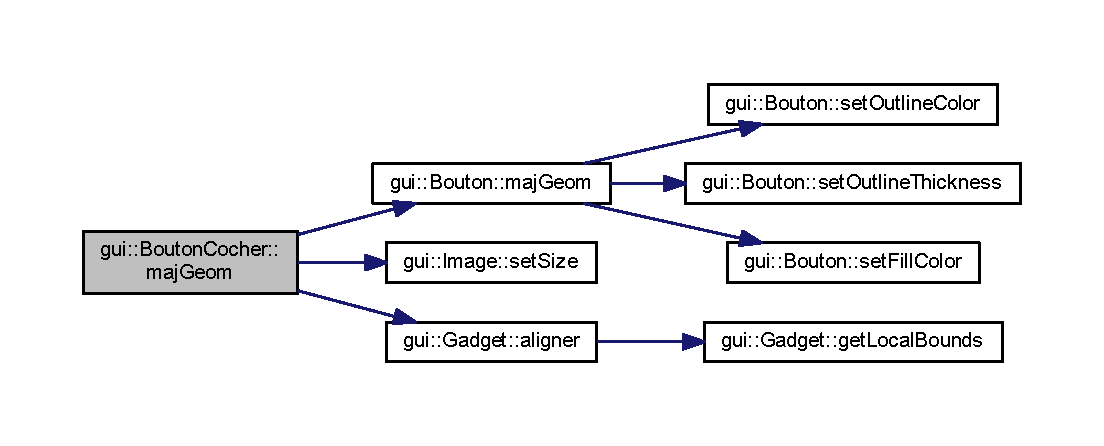
\includegraphics[width=350pt]{classgui_1_1_bouton_cocher_a03a7011fd1269a5502fd3b6e58652c4e_cgraph}
\end{center}
\end{figure}


\index{gui\+::\+Bouton\+Cocher@{gui\+::\+Bouton\+Cocher}!set\+Actif@{set\+Actif}}
\index{set\+Actif@{set\+Actif}!gui\+::\+Bouton\+Cocher@{gui\+::\+Bouton\+Cocher}}
\subsubsection[{set\+Actif(bool actif)}]{\setlength{\rightskip}{0pt plus 5cm}void gui\+::\+Bouton\+Cocher\+::set\+Actif (
\begin{DoxyParamCaption}
\item[{bool}]{actif}
\end{DoxyParamCaption}
)\hspace{0.3cm}{\ttfamily [inline]}}\label{classgui_1_1_bouton_cocher_ad8f3c398a2fb5c4f86b43dd9d9521c39}


Définir l\textquotesingle{}état du bouton. 


\begin{DoxyParams}{Paramètres}
{\em actif} & true \+: coché, false \+: décoché. \\
\hline
\end{DoxyParams}


\subsection{Documentation des champs}
\index{gui\+::\+Bouton\+Cocher@{gui\+::\+Bouton\+Cocher}!m\+\_\+actif@{m\+\_\+actif}}
\index{m\+\_\+actif@{m\+\_\+actif}!gui\+::\+Bouton\+Cocher@{gui\+::\+Bouton\+Cocher}}
\subsubsection[{m\+\_\+actif}]{\setlength{\rightskip}{0pt plus 5cm}bool gui\+::\+Bouton\+Cocher\+::m\+\_\+actif\hspace{0.3cm}{\ttfamily [private]}}\label{classgui_1_1_bouton_cocher_a96e4be65c04e461c51a6450a8caff484}


l\textquotesingle{}état du bouton (true\+: coché ou false\+:décoché). 

\index{gui\+::\+Bouton\+Cocher@{gui\+::\+Bouton\+Cocher}!m\+\_\+fct\+Toggle@{m\+\_\+fct\+Toggle}}
\index{m\+\_\+fct\+Toggle@{m\+\_\+fct\+Toggle}!gui\+::\+Bouton\+Cocher@{gui\+::\+Bouton\+Cocher}}
\subsubsection[{m\+\_\+fct\+Toggle}]{\setlength{\rightskip}{0pt plus 5cm}{\bf Func\+Type} gui\+::\+Bouton\+Cocher\+::m\+\_\+fct\+Toggle\hspace{0.3cm}{\ttfamily [private]}}\label{classgui_1_1_bouton_cocher_a944c1babbb13bb9dc5515c79fabc8780}


la fonction qui change l\textquotesingle{}état du bouton a chaque clique. 

\index{gui\+::\+Bouton\+Cocher@{gui\+::\+Bouton\+Cocher}!m\+\_\+img\+Coche@{m\+\_\+img\+Coche}}
\index{m\+\_\+img\+Coche@{m\+\_\+img\+Coche}!gui\+::\+Bouton\+Cocher@{gui\+::\+Bouton\+Cocher}}
\subsubsection[{m\+\_\+img\+Coche}]{\setlength{\rightskip}{0pt plus 5cm}{\bf Image}$\ast$ gui\+::\+Bouton\+Cocher\+::m\+\_\+img\+Coche\hspace{0.3cm}{\ttfamily [private]}}\label{classgui_1_1_bouton_cocher_a5a832444f9d527c678bcdcde9fb44d1a}


le gadget \doxyref{Image}{p.}{classgui_1_1_image} qui est visible si le bouton est coché. 



La documentation de cette classe a été générée à partir des fichiers suivants \+:\begin{DoxyCompactItemize}
\item 
Interface/include/gadgets/{\bf Bouton\+Cocher.\+h}\item 
Interface/src/gadgets/{\bf Bouton\+Cocher.\+cpp}\end{DoxyCompactItemize}

\section{Référence de la classe gui\+:\+:Bouton\+Texte}
\label{classgui_1_1_bouton_texte}\index{gui\+::\+Bouton\+Texte@{gui\+::\+Bouton\+Texte}}


\doxyref{Gadget}{p.}{classgui_1_1_gadget}, bouton rectangulaire (\doxyref{gui\+::\+Bouton}{p.}{classgui_1_1_bouton}) combiné à un \doxyref{Label}{p.}{classgui_1_1_label} (gui\+::texte).  




{\ttfamily \#include $<$Bouton\+Texte.\+h$>$}



Graphe d\textquotesingle{}héritage de gui\+:\+:Bouton\+Texte\+:\nopagebreak
\begin{figure}[H]
\begin{center}
\leavevmode
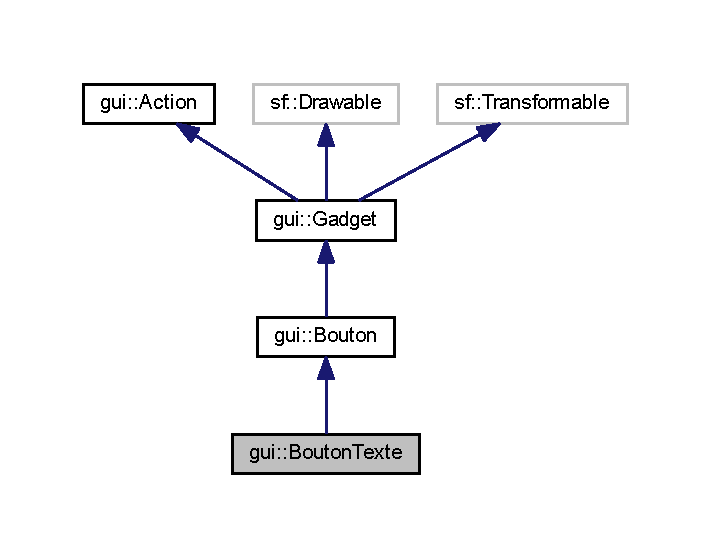
\includegraphics[width=341pt]{classgui_1_1_bouton_texte__inherit__graph}
\end{center}
\end{figure}


Graphe de collaboration de gui\+:\+:Bouton\+Texte\+:\nopagebreak
\begin{figure}[H]
\begin{center}
\leavevmode
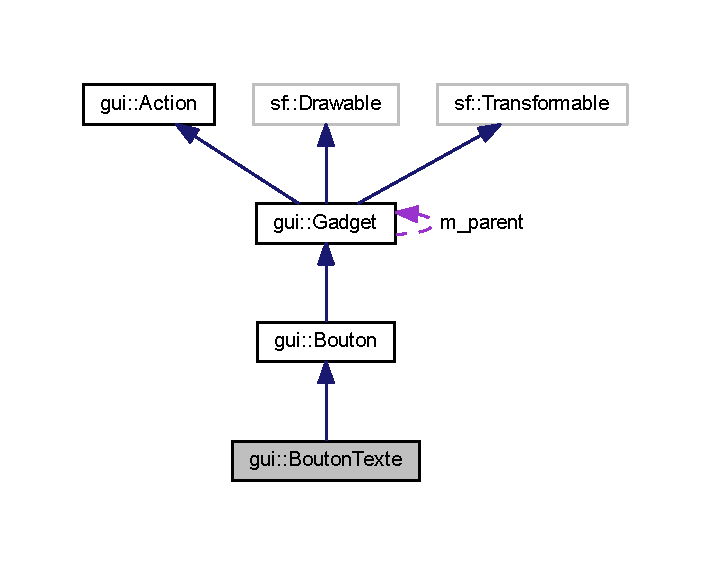
\includegraphics[width=341pt]{classgui_1_1_bouton_texte__coll__graph}
\end{center}
\end{figure}
\subsection*{Fonctions membres publiques}
\begin{DoxyCompactItemize}
\item 
{\bf Bouton\+Texte} (std\+::string texte=\char`\"{}\char`\"{})
\begin{DoxyCompactList}\small\item\em Constructeur défaut. \end{DoxyCompactList}\item 
{\bf Bouton\+Texte} (std\+::shared\+\_\+ptr$<$ {\bf Skin} $>$ skin, std\+::string texte=\char`\"{}\char`\"{})
\begin{DoxyCompactList}\small\item\em Constructeur a partir. \end{DoxyCompactList}\item 
virtual {\bf $\sim$\+Bouton\+Texte} ()
\begin{DoxyCompactList}\small\item\em Destructeur. \end{DoxyCompactList}\item 
void {\bf set\+Texte} (std\+::string texte)
\begin{DoxyCompactList}\small\item\em Definir le texte du bouton. \end{DoxyCompactList}\item 
std\+::string {\bf get\+Texte} ()
\begin{DoxyCompactList}\small\item\em Acceder au texte du bouton. \end{DoxyCompactList}\item 
void {\bf ajuster\+Au\+Texte} ()
\begin{DoxyCompactList}\small\item\em Ajuster la taille du bouton au texte du bouton (en tenant compte de la dimension de la bordure). \end{DoxyCompactList}\item 
virtual void {\bf set\+Size} (sf\+::\+Vector2f taille)
\begin{DoxyCompactList}\small\item\em Definir la taille du bouton. \end{DoxyCompactList}\item 
virtual void {\bf set\+Skin} (std\+::shared\+\_\+ptr$<$ {\bf Skin} $>$ skin)
\begin{DoxyCompactList}\small\item\em Definir le skin de reference du bouton. \end{DoxyCompactList}\item 
virtual void {\bf maj\+Geom} ()
\begin{DoxyCompactList}\small\item\em Actualise le style du label. \end{DoxyCompactList}\item 
virtual void {\bf draw} (sf\+::\+Render\+Target \&target, sf\+::\+Render\+States states) const 
\begin{DoxyCompactList}\small\item\em Rendre les éléments. \end{DoxyCompactList}\end{DoxyCompactItemize}
\subsection*{Attributs protégés}
\begin{DoxyCompactItemize}
\item 
std\+::shared\+\_\+ptr$<$ {\bf Label} $>$ {\bf m\+\_\+lbl\+Texte}
\begin{DoxyCompactList}\small\item\em pointeur vers le label. \end{DoxyCompactList}\end{DoxyCompactItemize}
\subsection*{Fonctions membres privées}
\begin{DoxyCompactItemize}
\item 
virtual void {\bf init} ()
\begin{DoxyCompactList}\small\item\em initialisation du gadget. \end{DoxyCompactList}\end{DoxyCompactItemize}
\subsection*{Membres hérités additionnels}


\subsection{Description détaillée}
\doxyref{Gadget}{p.}{classgui_1_1_gadget}, bouton rectangulaire (\doxyref{gui\+::\+Bouton}{p.}{classgui_1_1_bouton}) combiné à un \doxyref{Label}{p.}{classgui_1_1_label} (gui\+::texte). 

\begin{DoxySeeAlso}{Voir également}
\doxyref{gui\+::\+Gadget}{p.}{classgui_1_1_gadget} 
\end{DoxySeeAlso}


\subsection{Documentation des constructeurs et destructeur}
\index{gui\+::\+Bouton\+Texte@{gui\+::\+Bouton\+Texte}!Bouton\+Texte@{Bouton\+Texte}}
\index{Bouton\+Texte@{Bouton\+Texte}!gui\+::\+Bouton\+Texte@{gui\+::\+Bouton\+Texte}}
\subsubsection[{Bouton\+Texte(std\+::string texte="""")}]{\setlength{\rightskip}{0pt plus 5cm}gui\+::\+Bouton\+Texte\+::\+Bouton\+Texte (
\begin{DoxyParamCaption}
\item[{std\+::string}]{texte = {\ttfamily \char`\"{}\char`\"{}}}
\end{DoxyParamCaption}
)}\label{classgui_1_1_bouton_texte_a5781fca8e5397fad46a7e7ca0ba39c48}


Constructeur défaut. 

Creer le bouton avec la possibilité de définir le texte affiché.


\begin{DoxyParams}{Paramètres}
{\em texte} & le texte du bouton. (optionnel) \\
\hline
\end{DoxyParams}


Voici le graphe d\textquotesingle{}appel pour cette fonction \+:\nopagebreak
\begin{figure}[H]
\begin{center}
\leavevmode
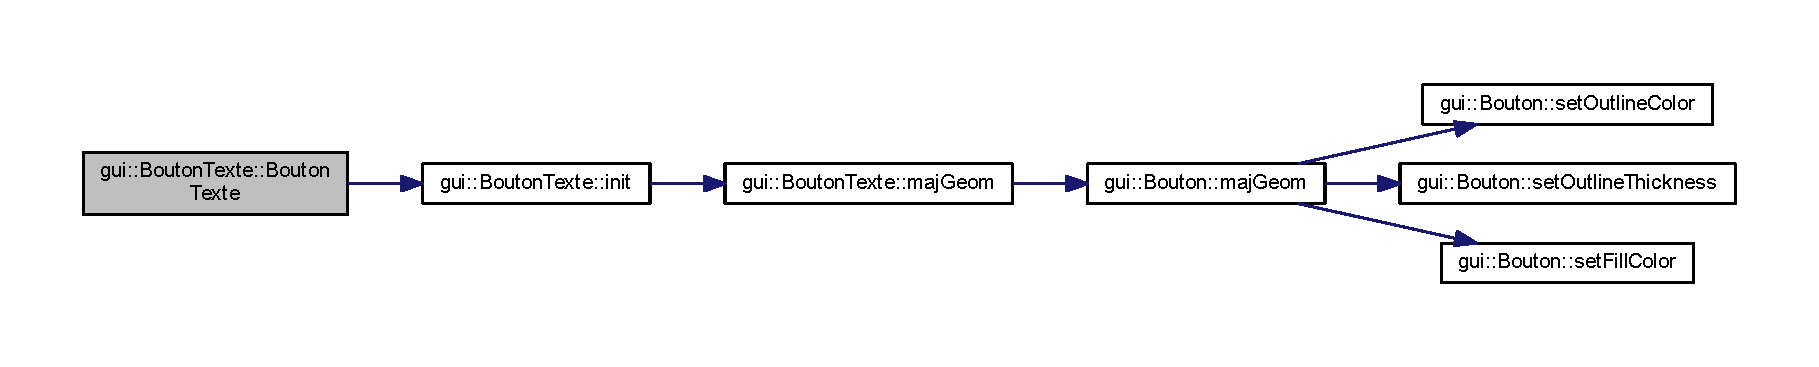
\includegraphics[width=350pt]{classgui_1_1_bouton_texte_a5781fca8e5397fad46a7e7ca0ba39c48_cgraph}
\end{center}
\end{figure}


\index{gui\+::\+Bouton\+Texte@{gui\+::\+Bouton\+Texte}!Bouton\+Texte@{Bouton\+Texte}}
\index{Bouton\+Texte@{Bouton\+Texte}!gui\+::\+Bouton\+Texte@{gui\+::\+Bouton\+Texte}}
\subsubsection[{Bouton\+Texte(std\+::shared\+\_\+ptr$<$ Skin $>$ skin, std\+::string texte="""")}]{\setlength{\rightskip}{0pt plus 5cm}gui\+::\+Bouton\+Texte\+::\+Bouton\+Texte (
\begin{DoxyParamCaption}
\item[{std\+::shared\+\_\+ptr$<$ {\bf Skin} $>$}]{skin, }
\item[{std\+::string}]{texte = {\ttfamily \char`\"{}\char`\"{}}}
\end{DoxyParamCaption}
)}\label{classgui_1_1_bouton_texte_a3372d6e64187d162203dc1ca3081243b}


Constructeur a partir. 


\begin{DoxyParams}{Paramètres}
{\em skin} & le skin à utilisé pour ce bouton. \\
\hline
{\em texte} & le texte du bouton. (optionnel) \\
\hline
\end{DoxyParams}
\begin{DoxyReturn}{Renvoie}

\end{DoxyReturn}


Voici le graphe d\textquotesingle{}appel pour cette fonction \+:\nopagebreak
\begin{figure}[H]
\begin{center}
\leavevmode
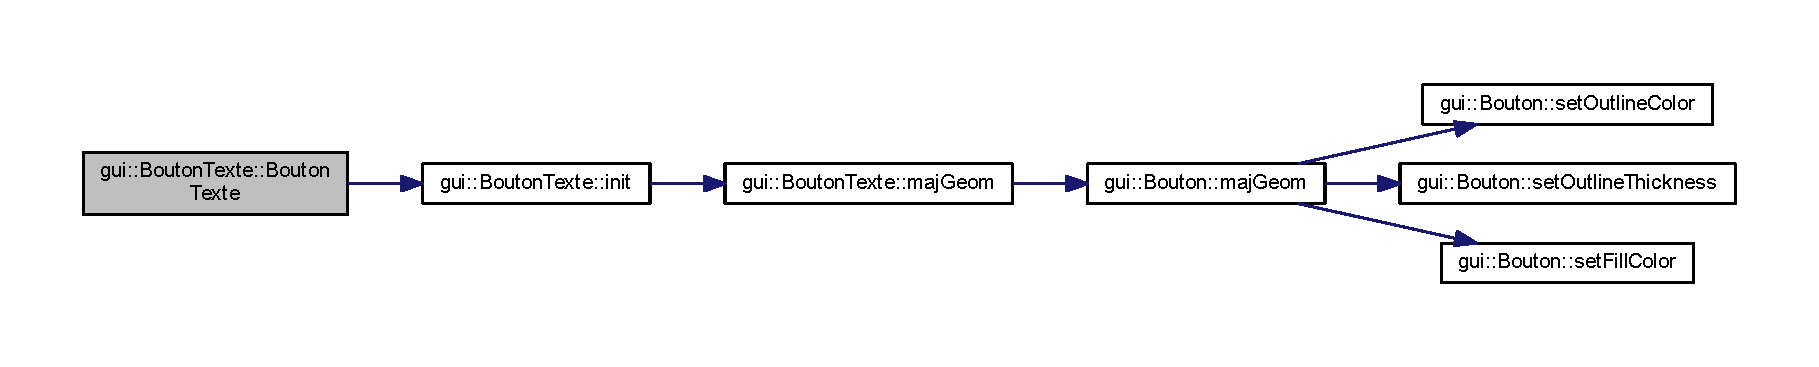
\includegraphics[width=350pt]{classgui_1_1_bouton_texte_a3372d6e64187d162203dc1ca3081243b_cgraph}
\end{center}
\end{figure}


\index{gui\+::\+Bouton\+Texte@{gui\+::\+Bouton\+Texte}!````~Bouton\+Texte@{$\sim$\+Bouton\+Texte}}
\index{````~Bouton\+Texte@{$\sim$\+Bouton\+Texte}!gui\+::\+Bouton\+Texte@{gui\+::\+Bouton\+Texte}}
\subsubsection[{$\sim$\+Bouton\+Texte()}]{\setlength{\rightskip}{0pt plus 5cm}gui\+::\+Bouton\+Texte\+::$\sim$\+Bouton\+Texte (
\begin{DoxyParamCaption}
{}
\end{DoxyParamCaption}
)\hspace{0.3cm}{\ttfamily [virtual]}}\label{classgui_1_1_bouton_texte_a33a4ef764ce7fe025f3d778274766d32}


Destructeur. 



\subsection{Documentation des fonctions membres}
\index{gui\+::\+Bouton\+Texte@{gui\+::\+Bouton\+Texte}!ajuster\+Au\+Texte@{ajuster\+Au\+Texte}}
\index{ajuster\+Au\+Texte@{ajuster\+Au\+Texte}!gui\+::\+Bouton\+Texte@{gui\+::\+Bouton\+Texte}}
\subsubsection[{ajuster\+Au\+Texte()}]{\setlength{\rightskip}{0pt plus 5cm}void gui\+::\+Bouton\+Texte\+::ajuster\+Au\+Texte (
\begin{DoxyParamCaption}
{}
\end{DoxyParamCaption}
)}\label{classgui_1_1_bouton_texte_a8d66645787dd0199b909b5fd52135c87}


Ajuster la taille du bouton au texte du bouton (en tenant compte de la dimension de la bordure). 

\index{gui\+::\+Bouton\+Texte@{gui\+::\+Bouton\+Texte}!draw@{draw}}
\index{draw@{draw}!gui\+::\+Bouton\+Texte@{gui\+::\+Bouton\+Texte}}
\subsubsection[{draw(sf\+::\+Render\+Target \&target, sf\+::\+Render\+States states) const }]{\setlength{\rightskip}{0pt plus 5cm}void gui\+::\+Bouton\+Texte\+::draw (
\begin{DoxyParamCaption}
\item[{sf\+::\+Render\+Target \&}]{target, }
\item[{sf\+::\+Render\+States}]{states}
\end{DoxyParamCaption}
) const\hspace{0.3cm}{\ttfamily [virtual]}}\label{classgui_1_1_bouton_texte_ac07e5e027d4d9d3544e8964d5d370714}


Rendre les éléments. 

Dessiner les différents éléments du ou des écrans actifs. \begin{DoxyReturn}{Renvoie}
Rien 
\end{DoxyReturn}


Réimplémentée à partir de {\bf gui\+::\+Bouton} \doxyref{}{p.}{classgui_1_1_bouton_a8d736a0c912d7bb23551ccc0aaa0e20d}.

\index{gui\+::\+Bouton\+Texte@{gui\+::\+Bouton\+Texte}!get\+Texte@{get\+Texte}}
\index{get\+Texte@{get\+Texte}!gui\+::\+Bouton\+Texte@{gui\+::\+Bouton\+Texte}}
\subsubsection[{get\+Texte()}]{\setlength{\rightskip}{0pt plus 5cm}std\+::string gui\+::\+Bouton\+Texte\+::get\+Texte (
\begin{DoxyParamCaption}
{}
\end{DoxyParamCaption}
)\hspace{0.3cm}{\ttfamily [inline]}}\label{classgui_1_1_bouton_texte_ac4b5e2d15656cbc05f0a2d07bd77762d}


Acceder au texte du bouton. 

\begin{DoxyReturn}{Renvoie}
la taille 
\end{DoxyReturn}
\index{gui\+::\+Bouton\+Texte@{gui\+::\+Bouton\+Texte}!init@{init}}
\index{init@{init}!gui\+::\+Bouton\+Texte@{gui\+::\+Bouton\+Texte}}
\subsubsection[{init()}]{\setlength{\rightskip}{0pt plus 5cm}void gui\+::\+Bouton\+Texte\+::init (
\begin{DoxyParamCaption}
{}
\end{DoxyParamCaption}
)\hspace{0.3cm}{\ttfamily [private]}, {\ttfamily [virtual]}}\label{classgui_1_1_bouton_texte_a2ee4ed04c1e2a20836e38a250d56311e}


initialisation du gadget. 

\begin{DoxyReturn}{Renvoie}
Rien 
\end{DoxyReturn}


Voici le graphe d\textquotesingle{}appel pour cette fonction \+:\nopagebreak
\begin{figure}[H]
\begin{center}
\leavevmode
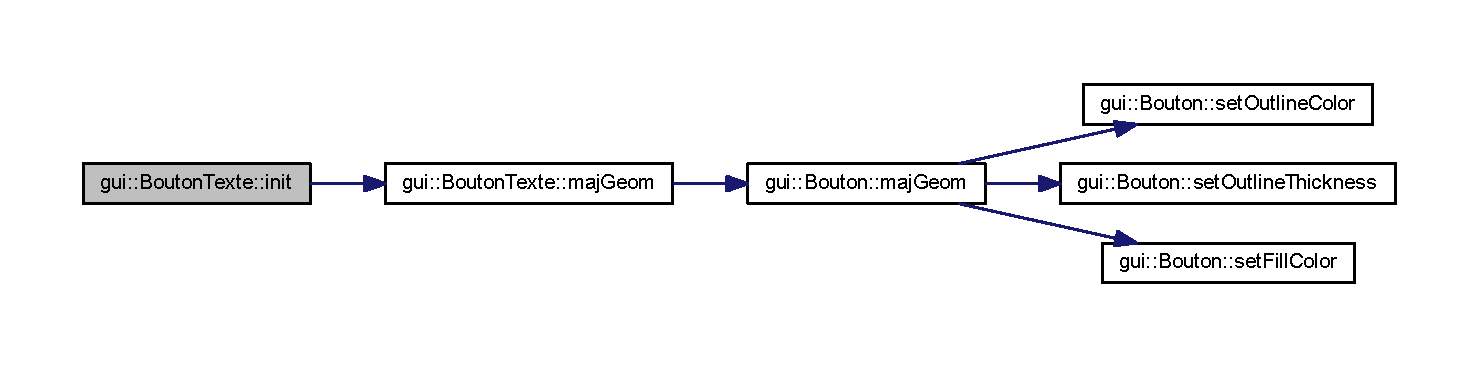
\includegraphics[width=350pt]{classgui_1_1_bouton_texte_a2ee4ed04c1e2a20836e38a250d56311e_cgraph}
\end{center}
\end{figure}




Voici le graphe des appelants de cette fonction \+:\nopagebreak
\begin{figure}[H]
\begin{center}
\leavevmode
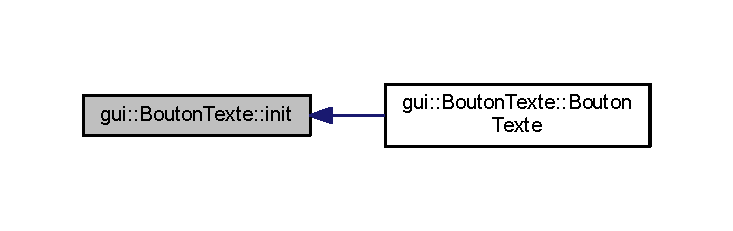
\includegraphics[width=350pt]{classgui_1_1_bouton_texte_a2ee4ed04c1e2a20836e38a250d56311e_icgraph}
\end{center}
\end{figure}


\index{gui\+::\+Bouton\+Texte@{gui\+::\+Bouton\+Texte}!maj\+Geom@{maj\+Geom}}
\index{maj\+Geom@{maj\+Geom}!gui\+::\+Bouton\+Texte@{gui\+::\+Bouton\+Texte}}
\subsubsection[{maj\+Geom()}]{\setlength{\rightskip}{0pt plus 5cm}void gui\+::\+Bouton\+Texte\+::maj\+Geom (
\begin{DoxyParamCaption}
{}
\end{DoxyParamCaption}
)\hspace{0.3cm}{\ttfamily [virtual]}}\label{classgui_1_1_bouton_texte_a6c66a5e34585fdb6054c2f56160db0a7}


Actualise le style du label. 



Réimplémentée à partir de {\bf gui\+::\+Bouton} \doxyref{}{p.}{classgui_1_1_bouton_a1ff3d7a1586eaab5873cc6e49be2332c}.



Voici le graphe d\textquotesingle{}appel pour cette fonction \+:\nopagebreak
\begin{figure}[H]
\begin{center}
\leavevmode
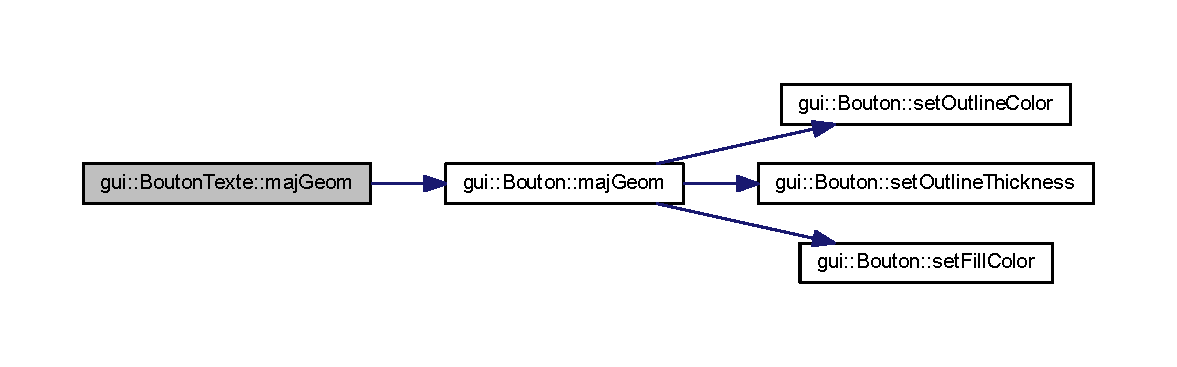
\includegraphics[width=350pt]{classgui_1_1_bouton_texte_a6c66a5e34585fdb6054c2f56160db0a7_cgraph}
\end{center}
\end{figure}




Voici le graphe des appelants de cette fonction \+:\nopagebreak
\begin{figure}[H]
\begin{center}
\leavevmode
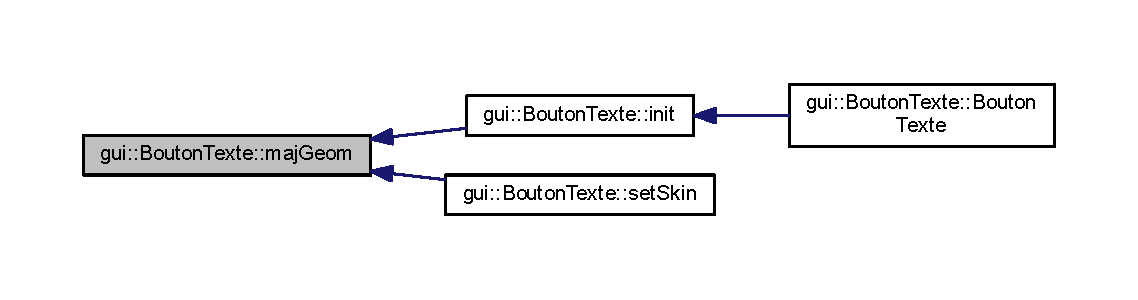
\includegraphics[width=350pt]{classgui_1_1_bouton_texte_a6c66a5e34585fdb6054c2f56160db0a7_icgraph}
\end{center}
\end{figure}


\index{gui\+::\+Bouton\+Texte@{gui\+::\+Bouton\+Texte}!set\+Size@{set\+Size}}
\index{set\+Size@{set\+Size}!gui\+::\+Bouton\+Texte@{gui\+::\+Bouton\+Texte}}
\subsubsection[{set\+Size(sf\+::\+Vector2f taille)}]{\setlength{\rightskip}{0pt plus 5cm}void gui\+::\+Bouton\+Texte\+::set\+Size (
\begin{DoxyParamCaption}
\item[{sf\+::\+Vector2f}]{taille}
\end{DoxyParamCaption}
)\hspace{0.3cm}{\ttfamily [virtual]}}\label{classgui_1_1_bouton_texte_a1725dffd7f645561ee4db8786d83a85e}


Definir la taille du bouton. 


\begin{DoxyParams}{Paramètres}
{\em taille} & La nouvelle taille. \\
\hline
\end{DoxyParams}


Réimplémentée à partir de {\bf gui\+::\+Bouton} \doxyref{}{p.}{classgui_1_1_bouton_a7652dfbbb1180cfecc0db6b68db38776}.

\index{gui\+::\+Bouton\+Texte@{gui\+::\+Bouton\+Texte}!set\+Skin@{set\+Skin}}
\index{set\+Skin@{set\+Skin}!gui\+::\+Bouton\+Texte@{gui\+::\+Bouton\+Texte}}
\subsubsection[{set\+Skin(std\+::shared\+\_\+ptr$<$ Skin $>$ skin)}]{\setlength{\rightskip}{0pt plus 5cm}void gui\+::\+Bouton\+Texte\+::set\+Skin (
\begin{DoxyParamCaption}
\item[{std\+::shared\+\_\+ptr$<$ {\bf Skin} $>$}]{skin}
\end{DoxyParamCaption}
)\hspace{0.3cm}{\ttfamily [virtual]}}\label{classgui_1_1_bouton_texte_ab8059cd7c83e678dd8b3c9dba62a2363}


Definir le skin de reference du bouton. 


\begin{DoxyParams}{Paramètres}
{\em skin} & La nouvelle taille. \\
\hline
\end{DoxyParams}


Réimplémentée à partir de {\bf gui\+::\+Bouton} \doxyref{}{p.}{classgui_1_1_bouton_aba971350f784988e1a03328264e551bb}.



Voici le graphe d\textquotesingle{}appel pour cette fonction \+:\nopagebreak
\begin{figure}[H]
\begin{center}
\leavevmode
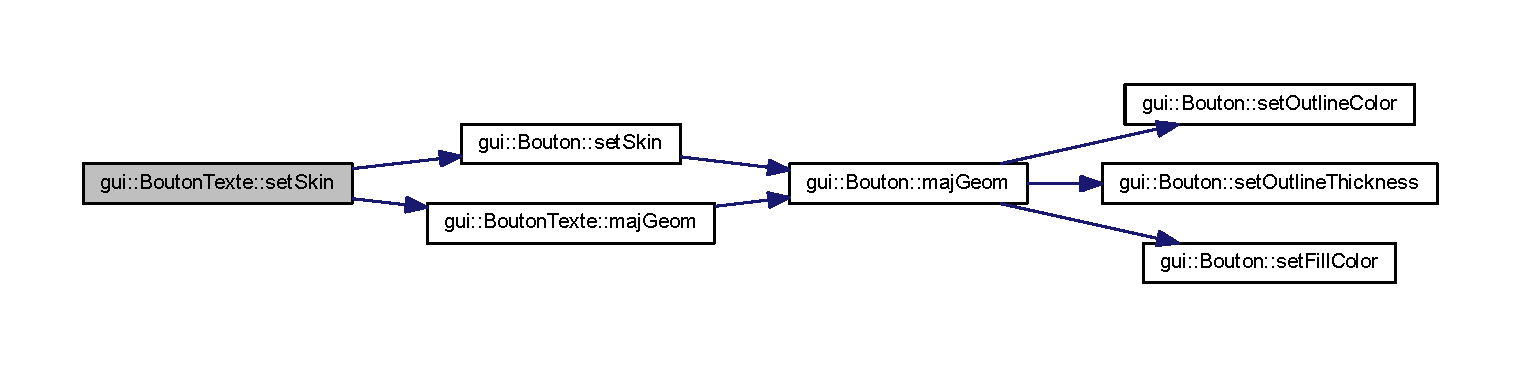
\includegraphics[width=350pt]{classgui_1_1_bouton_texte_ab8059cd7c83e678dd8b3c9dba62a2363_cgraph}
\end{center}
\end{figure}


\index{gui\+::\+Bouton\+Texte@{gui\+::\+Bouton\+Texte}!set\+Texte@{set\+Texte}}
\index{set\+Texte@{set\+Texte}!gui\+::\+Bouton\+Texte@{gui\+::\+Bouton\+Texte}}
\subsubsection[{set\+Texte(std\+::string texte)}]{\setlength{\rightskip}{0pt plus 5cm}void gui\+::\+Bouton\+Texte\+::set\+Texte (
\begin{DoxyParamCaption}
\item[{std\+::string}]{texte}
\end{DoxyParamCaption}
)\hspace{0.3cm}{\ttfamily [inline]}}\label{classgui_1_1_bouton_texte_a6c4fcc7a5b0be6317245387d6078fb88}


Definir le texte du bouton. 


\begin{DoxyParams}{Paramètres}
{\em texte} & le texte du bouton. \\
\hline
\end{DoxyParams}


\subsection{Documentation des champs}
\index{gui\+::\+Bouton\+Texte@{gui\+::\+Bouton\+Texte}!m\+\_\+lbl\+Texte@{m\+\_\+lbl\+Texte}}
\index{m\+\_\+lbl\+Texte@{m\+\_\+lbl\+Texte}!gui\+::\+Bouton\+Texte@{gui\+::\+Bouton\+Texte}}
\subsubsection[{m\+\_\+lbl\+Texte}]{\setlength{\rightskip}{0pt plus 5cm}std\+::shared\+\_\+ptr$<${\bf Label}$>$ gui\+::\+Bouton\+Texte\+::m\+\_\+lbl\+Texte\hspace{0.3cm}{\ttfamily [protected]}}\label{classgui_1_1_bouton_texte_adedb7fc1377556a249211d9724f702f9}


pointeur vers le label. 



La documentation de cette classe a été générée à partir des fichiers suivants \+:\begin{DoxyCompactItemize}
\item 
Interface/include/gadgets/{\bf Bouton\+Texte.\+h}\item 
Interface/src/gadgets/{\bf Bouton\+Texte.\+cpp}\end{DoxyCompactItemize}

\section{Référence de la classe app\+:\+:Config}
\label{classapp_1_1_config}\index{app\+::\+Config@{app\+::\+Config}}


Contient les différents éléments de Configuration de l\textquotesingle{}application.  




{\ttfamily \#include $<$Config.\+h$>$}



Graphe de collaboration de app\+:\+:Config\+:\nopagebreak
\begin{figure}[H]
\begin{center}
\leavevmode
\includegraphics[width=324pt]{classapp_1_1_config__coll__graph}
\end{center}
\end{figure}
\subsection*{Types publics}
\begin{DoxyCompactItemize}
\item 
enum {\bf Polices} \+: int \{ {\bf police\+\_\+1}, 
{\bf police\+\_\+2}
 \}\begin{DoxyCompactList}\small\item\em listes les polices enregistrable dans le manager de polices \end{DoxyCompactList}
\item 
enum {\bf Styles} \+: int \{ {\bf root}, 
{\bf Bouton}, 
{\bf Fenetre}
 \}\begin{DoxyCompactList}\small\item\em listes les styles (\doxyref{gui\+::\+Style}{p.}{structgui_1_1_style}) enregistrable dans la pile des Styles \end{DoxyCompactList}
\item 
enum {\bf Skins} \+: int \{ {\bf Skin1}
 \}\begin{DoxyCompactList}\small\item\em listes les skins (\doxyref{gui\+::\+Skin}{p.}{structgui_1_1_skin}) enregistrable dans la pile des skins. \end{DoxyCompactList}
\end{DoxyCompactItemize}
\subsection*{Fonctions membres publiques}
\begin{DoxyCompactItemize}
\item 
{\bf Config} ()
\begin{DoxyCompactList}\small\item\em Constructeur. \end{DoxyCompactList}\item 
virtual {\bf $\sim$\+Config} ()
\begin{DoxyCompactList}\small\item\em Destructeur. \end{DoxyCompactList}\end{DoxyCompactItemize}
\subsection*{Fonctions membres publiques statiques}
\begin{DoxyCompactItemize}
\item 
static void {\bf init} ()
\begin{DoxyCompactList}\small\item\em Initialiser les differents élément. \end{DoxyCompactList}\item 
static sf\+::\+Time {\bf get\+Duree\+Image} ()
\begin{DoxyCompactList}\small\item\em recuperer la durée d\textquotesingle{}une image, Duree\+Image = 1.\+f / 60.\+f à 60\+Fps. \end{DoxyCompactList}\end{DoxyCompactItemize}
\subsection*{Attributs publics statiques}
\begin{DoxyCompactItemize}
\item 
static {\bf Resource\+Mgr}$<$ sf\+::\+Texture, int $>$ {\bf m\+\_\+textures}
\begin{DoxyCompactList}\small\item\em Manager des textures. \end{DoxyCompactList}\item 
static {\bf Resource\+Mgr}$<$ sf\+::\+Font, int $>$ {\bf m\+\_\+polices}
\begin{DoxyCompactList}\small\item\em Manager des polices. \end{DoxyCompactList}\item 
static std\+::map$<$ {\bf Styles}, std\+::shared\+\_\+ptr$<$ {\bf gui\+::\+Style} $>$ $>$ {\bf m\+\_\+styles} = \{\}
\begin{DoxyCompactList}\small\item\em les styles pour le G\+U\+I \end{DoxyCompactList}\item 
static std\+::map$<$ {\bf Skins}, std\+::shared\+\_\+ptr$<$ {\bf gui\+::\+Skin} $>$ $>$ {\bf m\+\_\+skins} = \{\}
\begin{DoxyCompactList}\small\item\em les styles pour le G\+U\+I \end{DoxyCompactList}\end{DoxyCompactItemize}
\subsection*{Fonctions membres privées statiques}
\begin{DoxyCompactItemize}
\item 
static void {\bf init\+Textures} ()
\begin{DoxyCompactList}\small\item\em Initialise le manager de textures. \end{DoxyCompactList}\item 
static void {\bf init\+Polices} ()
\begin{DoxyCompactList}\small\item\em Initialise le Manager des polices. \end{DoxyCompactList}\item 
static void {\bf init\+Skins} ()
\begin{DoxyCompactList}\small\item\em Initialiser les differents skins pour l\textquotesingle{}interface graphique. \end{DoxyCompactList}\item 
static void {\bf init\+Styles} ()
\begin{DoxyCompactList}\small\item\em Initialiser les differents styles pour l\textquotesingle{}interface graphique. \end{DoxyCompactList}\end{DoxyCompactItemize}
\subsection*{Attributs privés statiques}
\begin{DoxyCompactItemize}
\item 
static sf\+::\+Time {\bf m\+\_\+duree\+Image}
\begin{DoxyCompactList}\small\item\em Durée d\textquotesingle{}une image, Autrement dit on a 1/\+Frame\+Rate = {\itshape Duree\+Image}. \end{DoxyCompactList}\end{DoxyCompactItemize}


\subsection{Description détaillée}
Contient les différents éléments de Configuration de l\textquotesingle{}application. 

Configuration des textures, sons, musiques polices, tailles, couleurs ....

\begin{DoxySeeAlso}{Voir également}
\doxyref{app\+::\+Ecran}{p.}{classapp_1_1_ecran}, \doxyref{app\+::\+Gestion\+\_\+ecrans}{p.}{classapp_1_1_gestion__ecrans} 
\end{DoxySeeAlso}


\subsection{Documentation des énumérations membres}
\index{app\+::\+Config@{app\+::\+Config}!Polices@{Polices}}
\index{Polices@{Polices}!app\+::\+Config@{app\+::\+Config}}
\subsubsection[{Polices}]{\setlength{\rightskip}{0pt plus 5cm}enum {\bf app\+::\+Config\+::\+Polices} \+: int}\label{classapp_1_1_config_ac576a323feff0b9aaa6aecd40e038049}


listes les polices enregistrable dans le manager de polices 

\begin{Desc}
\item[Valeurs énumérées]\par
\begin{description}
\index{police\+\_\+1@{police\+\_\+1}!app\+::\+Config@{app\+::\+Config}}\index{app\+::\+Config@{app\+::\+Config}!police\+\_\+1@{police\+\_\+1}}\item[{\em 
police\+\_\+1\label{classapp_1_1_config_ac576a323feff0b9aaa6aecd40e038049a759ba1bca9923fc3b3e61b9e0edd154a}
}]\index{police\+\_\+2@{police\+\_\+2}!app\+::\+Config@{app\+::\+Config}}\index{app\+::\+Config@{app\+::\+Config}!police\+\_\+2@{police\+\_\+2}}\item[{\em 
police\+\_\+2\label{classapp_1_1_config_ac576a323feff0b9aaa6aecd40e038049abd01fcbe87968783a525da9dc5ef0f21}
}]\end{description}
\end{Desc}
\index{app\+::\+Config@{app\+::\+Config}!Skins@{Skins}}
\index{Skins@{Skins}!app\+::\+Config@{app\+::\+Config}}
\subsubsection[{Skins}]{\setlength{\rightskip}{0pt plus 5cm}enum {\bf app\+::\+Config\+::\+Skins} \+: int}\label{classapp_1_1_config_a457412fb51e1853408f2201a69471e32}


listes les skins (\doxyref{gui\+::\+Skin}{p.}{structgui_1_1_skin}) enregistrable dans la pile des skins. 

\begin{Desc}
\item[Valeurs énumérées]\par
\begin{description}
\index{Skin1@{Skin1}!app\+::\+Config@{app\+::\+Config}}\index{app\+::\+Config@{app\+::\+Config}!Skin1@{Skin1}}\item[{\em 
Skin1\label{classapp_1_1_config_a457412fb51e1853408f2201a69471e32abb0a28eb4da75e2aadaf74b6d9aa2d4e}
}]\end{description}
\end{Desc}
\index{app\+::\+Config@{app\+::\+Config}!Styles@{Styles}}
\index{Styles@{Styles}!app\+::\+Config@{app\+::\+Config}}
\subsubsection[{Styles}]{\setlength{\rightskip}{0pt plus 5cm}enum {\bf app\+::\+Config\+::\+Styles} \+: int}\label{classapp_1_1_config_ab0fd2b7fe87a4b68c93d2a4a7209beda}


listes les styles (\doxyref{gui\+::\+Style}{p.}{structgui_1_1_style}) enregistrable dans la pile des Styles 

\begin{Desc}
\item[Valeurs énumérées]\par
\begin{description}
\index{root@{root}!app\+::\+Config@{app\+::\+Config}}\index{app\+::\+Config@{app\+::\+Config}!root@{root}}\item[{\em 
root\label{classapp_1_1_config_ab0fd2b7fe87a4b68c93d2a4a7209bedaa02fd230360f0a9b4e42a24c2e826e2a7}
}]\index{Bouton@{Bouton}!app\+::\+Config@{app\+::\+Config}}\index{app\+::\+Config@{app\+::\+Config}!Bouton@{Bouton}}\item[{\em 
Bouton\label{classapp_1_1_config_ab0fd2b7fe87a4b68c93d2a4a7209bedaa853b0170848ebe1bb8aa66895283a816}
}]\index{Fenetre@{Fenetre}!app\+::\+Config@{app\+::\+Config}}\index{app\+::\+Config@{app\+::\+Config}!Fenetre@{Fenetre}}\item[{\em 
Fenetre\label{classapp_1_1_config_ab0fd2b7fe87a4b68c93d2a4a7209bedaa1297561847b1b84d487c3a875f5f8f6a}
}]\end{description}
\end{Desc}


\subsection{Documentation des constructeurs et destructeur}
\index{app\+::\+Config@{app\+::\+Config}!Config@{Config}}
\index{Config@{Config}!app\+::\+Config@{app\+::\+Config}}
\subsubsection[{Config()}]{\setlength{\rightskip}{0pt plus 5cm}app\+::\+Config\+::\+Config (
\begin{DoxyParamCaption}
{}
\end{DoxyParamCaption}
)}\label{classapp_1_1_config_a6b5877b87cbfef7bb28ed405dfa3ea62}


Constructeur. 

\index{app\+::\+Config@{app\+::\+Config}!````~Config@{$\sim$\+Config}}
\index{````~Config@{$\sim$\+Config}!app\+::\+Config@{app\+::\+Config}}
\subsubsection[{$\sim$\+Config()}]{\setlength{\rightskip}{0pt plus 5cm}app\+::\+Config\+::$\sim$\+Config (
\begin{DoxyParamCaption}
{}
\end{DoxyParamCaption}
)\hspace{0.3cm}{\ttfamily [virtual]}}\label{classapp_1_1_config_a44e97c97554890ab2ef671855d90dbbc}


Destructeur. 



\subsection{Documentation des fonctions membres}
\index{app\+::\+Config@{app\+::\+Config}!get\+Duree\+Image@{get\+Duree\+Image}}
\index{get\+Duree\+Image@{get\+Duree\+Image}!app\+::\+Config@{app\+::\+Config}}
\subsubsection[{get\+Duree\+Image()}]{\setlength{\rightskip}{0pt plus 5cm}sf\+::\+Time app\+::\+Config\+::get\+Duree\+Image (
\begin{DoxyParamCaption}
{}
\end{DoxyParamCaption}
)\hspace{0.3cm}{\ttfamily [static]}}\label{classapp_1_1_config_a300d3ecafed165cfe44b93c555116ff5}


recuperer la durée d\textquotesingle{}une image, Duree\+Image = 1.\+f / 60.\+f à 60\+Fps. 



Voici le graphe des appelants de cette fonction \+:\nopagebreak
\begin{figure}[H]
\begin{center}
\leavevmode
\includegraphics[width=350pt]{classapp_1_1_config_a300d3ecafed165cfe44b93c555116ff5_icgraph}
\end{center}
\end{figure}


\index{app\+::\+Config@{app\+::\+Config}!init@{init}}
\index{init@{init}!app\+::\+Config@{app\+::\+Config}}
\subsubsection[{init()}]{\setlength{\rightskip}{0pt plus 5cm}void app\+::\+Config\+::init (
\begin{DoxyParamCaption}
{}
\end{DoxyParamCaption}
)\hspace{0.3cm}{\ttfamily [static]}}\label{classapp_1_1_config_a48395c7e382fb68f5283676847b4fb58}


Initialiser les differents élément. 

\begin{DoxyItemize}
\item les textures \item les polices \item les styles \item les sons (à prévoir) \item les musiques (à prévoir) \end{DoxyItemize}


Voici le graphe d\textquotesingle{}appel pour cette fonction \+:\nopagebreak
\begin{figure}[H]
\begin{center}
\leavevmode
\includegraphics[width=350pt]{classapp_1_1_config_a48395c7e382fb68f5283676847b4fb58_cgraph}
\end{center}
\end{figure}




Voici le graphe des appelants de cette fonction \+:\nopagebreak
\begin{figure}[H]
\begin{center}
\leavevmode
\includegraphics[width=340pt]{classapp_1_1_config_a48395c7e382fb68f5283676847b4fb58_icgraph}
\end{center}
\end{figure}


\index{app\+::\+Config@{app\+::\+Config}!init\+Polices@{init\+Polices}}
\index{init\+Polices@{init\+Polices}!app\+::\+Config@{app\+::\+Config}}
\subsubsection[{init\+Polices()}]{\setlength{\rightskip}{0pt plus 5cm}void app\+::\+Config\+::init\+Polices (
\begin{DoxyParamCaption}
{}
\end{DoxyParamCaption}
)\hspace{0.3cm}{\ttfamily [static]}, {\ttfamily [private]}}\label{classapp_1_1_config_ada2a8a71c6ef00e4726666af45c04d25}


Initialise le Manager des polices. 



Voici le graphe des appelants de cette fonction \+:\nopagebreak
\begin{figure}[H]
\begin{center}
\leavevmode
\includegraphics[width=350pt]{classapp_1_1_config_ada2a8a71c6ef00e4726666af45c04d25_icgraph}
\end{center}
\end{figure}


\index{app\+::\+Config@{app\+::\+Config}!init\+Skins@{init\+Skins}}
\index{init\+Skins@{init\+Skins}!app\+::\+Config@{app\+::\+Config}}
\subsubsection[{init\+Skins()}]{\setlength{\rightskip}{0pt plus 5cm}void app\+::\+Config\+::init\+Skins (
\begin{DoxyParamCaption}
{}
\end{DoxyParamCaption}
)\hspace{0.3cm}{\ttfamily [static]}, {\ttfamily [private]}}\label{classapp_1_1_config_a87cba3dc8625eccfe14efae71555312c}


Initialiser les differents skins pour l\textquotesingle{}interface graphique. 



Voici le graphe d\textquotesingle{}appel pour cette fonction \+:\nopagebreak
\begin{figure}[H]
\begin{center}
\leavevmode
\includegraphics[width=341pt]{classapp_1_1_config_a87cba3dc8625eccfe14efae71555312c_cgraph}
\end{center}
\end{figure}




Voici le graphe des appelants de cette fonction \+:\nopagebreak
\begin{figure}[H]
\begin{center}
\leavevmode
\includegraphics[width=350pt]{classapp_1_1_config_a87cba3dc8625eccfe14efae71555312c_icgraph}
\end{center}
\end{figure}


\index{app\+::\+Config@{app\+::\+Config}!init\+Styles@{init\+Styles}}
\index{init\+Styles@{init\+Styles}!app\+::\+Config@{app\+::\+Config}}
\subsubsection[{init\+Styles()}]{\setlength{\rightskip}{0pt plus 5cm}void app\+::\+Config\+::init\+Styles (
\begin{DoxyParamCaption}
{}
\end{DoxyParamCaption}
)\hspace{0.3cm}{\ttfamily [static]}, {\ttfamily [private]}}\label{classapp_1_1_config_a3f6e6c60455e9b9f35fdead803864bcf}


Initialiser les differents styles pour l\textquotesingle{}interface graphique. 



Voici le graphe des appelants de cette fonction \+:\nopagebreak
\begin{figure}[H]
\begin{center}
\leavevmode
\includegraphics[width=350pt]{classapp_1_1_config_a3f6e6c60455e9b9f35fdead803864bcf_icgraph}
\end{center}
\end{figure}


\index{app\+::\+Config@{app\+::\+Config}!init\+Textures@{init\+Textures}}
\index{init\+Textures@{init\+Textures}!app\+::\+Config@{app\+::\+Config}}
\subsubsection[{init\+Textures()}]{\setlength{\rightskip}{0pt plus 5cm}void app\+::\+Config\+::init\+Textures (
\begin{DoxyParamCaption}
{}
\end{DoxyParamCaption}
)\hspace{0.3cm}{\ttfamily [static]}, {\ttfamily [private]}}\label{classapp_1_1_config_a690065179d9ef7ade6a67193f44acb89}


Initialise le manager de textures. 



Voici le graphe des appelants de cette fonction \+:\nopagebreak
\begin{figure}[H]
\begin{center}
\leavevmode
\includegraphics[width=350pt]{classapp_1_1_config_a690065179d9ef7ade6a67193f44acb89_icgraph}
\end{center}
\end{figure}




\subsection{Documentation des champs}
\index{app\+::\+Config@{app\+::\+Config}!m\+\_\+duree\+Image@{m\+\_\+duree\+Image}}
\index{m\+\_\+duree\+Image@{m\+\_\+duree\+Image}!app\+::\+Config@{app\+::\+Config}}
\subsubsection[{m\+\_\+duree\+Image}]{\setlength{\rightskip}{0pt plus 5cm}sf\+::\+Time app\+::\+Config\+::m\+\_\+duree\+Image\hspace{0.3cm}{\ttfamily [static]}, {\ttfamily [private]}}\label{classapp_1_1_config_a3cd597c93472e36b707e3cf2e3eb0d74}


Durée d\textquotesingle{}une image, Autrement dit on a 1/\+Frame\+Rate = {\itshape Duree\+Image}. 

\index{app\+::\+Config@{app\+::\+Config}!m\+\_\+polices@{m\+\_\+polices}}
\index{m\+\_\+polices@{m\+\_\+polices}!app\+::\+Config@{app\+::\+Config}}
\subsubsection[{m\+\_\+polices}]{\setlength{\rightskip}{0pt plus 5cm}{\bf Resource\+Mgr}$<$ sf\+::\+Font, int $>$ app\+::\+Config\+::m\+\_\+polices\hspace{0.3cm}{\ttfamily [static]}}\label{classapp_1_1_config_affadef60c92912efa871fff516f844de}


Manager des polices. 

\index{app\+::\+Config@{app\+::\+Config}!m\+\_\+skins@{m\+\_\+skins}}
\index{m\+\_\+skins@{m\+\_\+skins}!app\+::\+Config@{app\+::\+Config}}
\subsubsection[{m\+\_\+skins}]{\setlength{\rightskip}{0pt plus 5cm}std\+::map$<$ {\bf Config\+::\+Skins}, std\+::shared\+\_\+ptr$<$ {\bf gui\+::\+Skin} $>$ $>$ app\+::\+Config\+::m\+\_\+skins = \{\}\hspace{0.3cm}{\ttfamily [static]}}\label{classapp_1_1_config_a0f5031fe192ad475a316f76af23dad5b}


les styles pour le G\+U\+I 

\begin{DoxyRefDesc}{A faire}
\item[{\bf A faire}]passer de pointer$\ast$ à point shared\+\_\+ptr ou unique\+\_\+ptr ? \end{DoxyRefDesc}
\index{app\+::\+Config@{app\+::\+Config}!m\+\_\+styles@{m\+\_\+styles}}
\index{m\+\_\+styles@{m\+\_\+styles}!app\+::\+Config@{app\+::\+Config}}
\subsubsection[{m\+\_\+styles}]{\setlength{\rightskip}{0pt plus 5cm}std\+::map$<$ {\bf Config\+::\+Styles}, std\+::shared\+\_\+ptr$<$ {\bf gui\+::\+Style} $>$ $>$ app\+::\+Config\+::m\+\_\+styles = \{\}\hspace{0.3cm}{\ttfamily [static]}}\label{classapp_1_1_config_aca7399e3ebaf8448a94a809c471cd4e7}


les styles pour le G\+U\+I 

\begin{DoxyRefDesc}{A faire}
\item[{\bf A faire}]passer de pointer$\ast$ à point shared\+\_\+ptr ou unique\+\_\+ptr ? \end{DoxyRefDesc}
\index{app\+::\+Config@{app\+::\+Config}!m\+\_\+textures@{m\+\_\+textures}}
\index{m\+\_\+textures@{m\+\_\+textures}!app\+::\+Config@{app\+::\+Config}}
\subsubsection[{m\+\_\+textures}]{\setlength{\rightskip}{0pt plus 5cm}{\bf Resource\+Mgr}$<$sf\+::\+Texture,int$>$ app\+::\+Config\+::m\+\_\+textures\hspace{0.3cm}{\ttfamily [static]}}\label{classapp_1_1_config_a673cf82df5a28f6087aa1992a5667ce2}


Manager des textures. 



La documentation de cette classe a été générée à partir des fichiers suivants \+:\begin{DoxyCompactItemize}
\item 
main/include/{\bf Config.\+h}\item 
main/src/{\bf Config.\+cpp}\end{DoxyCompactItemize}

\section{Référence de la classe app\+:\+:Ecran}
\label{classapp_1_1_ecran}\index{app\+::\+Ecran@{app\+::\+Ecran}}


La classe virtuelle communues aux écrans.  




{\ttfamily \#include $<$Ecran.\+h$>$}



Graphe d\textquotesingle{}héritage de app\+:\+:Ecran\+:\nopagebreak
\begin{figure}[H]
\begin{center}
\leavevmode
\includegraphics[width=169pt]{classapp_1_1_ecran__inherit__graph}
\end{center}
\end{figure}


Graphe de collaboration de app\+:\+:Ecran\+:\nopagebreak
\begin{figure}[H]
\begin{center}
\leavevmode
\includegraphics[width=187pt]{classapp_1_1_ecran__coll__graph}
\end{center}
\end{figure}
\subsection*{Fonctions membres publiques}
\begin{DoxyCompactItemize}
\item 
{\bf Ecran} ({\bf Application} $\ast$appli)
\begin{DoxyCompactList}\small\item\em Constructeur. \end{DoxyCompactList}\item 
virtual {\bf $\sim$\+Ecran} ()
\begin{DoxyCompactList}\small\item\em Destructeur virtuel. \end{DoxyCompactList}\item 
virtual void {\bf traiter\+\_\+evenements} (const sf\+::\+Event \&event)=0
\begin{DoxyCompactList}\small\item\em Gère les entrées claviers, souris, fenetre ... \end{DoxyCompactList}\item 
virtual void {\bf actualiser} (float delta\+T)=0
\begin{DoxyCompactList}\small\item\em Actualiser les éléments. \end{DoxyCompactList}\item 
virtual void {\bf dessiner} ()=0
\begin{DoxyCompactList}\small\item\em Rendre les éléments. \end{DoxyCompactList}\end{DoxyCompactItemize}
\subsection*{Attributs protégés}
\begin{DoxyCompactItemize}
\item 
{\bf Application} $\ast$ {\bf m\+\_\+appli}
\begin{DoxyCompactList}\small\item\em La classe Apllication parent. \end{DoxyCompactList}\end{DoxyCompactItemize}


\subsection{Description détaillée}
La classe virtuelle communues aux écrans. 

\doxyref{app\+::\+Ecran}{p.}{classapp_1_1_ecran} la classe de base des écrans. Les écrans peuvent se superposer (par exemple l\textquotesingle{}écran pause-\/option avec en dessous l\textquotesingle{}écran jeu en pause).

\begin{DoxySeeAlso}{Voir également}
\doxyref{app\+::\+Ecran\+Demo}{p.}{classapp_1_1_ecran_demo} 
\end{DoxySeeAlso}


\subsection{Documentation des constructeurs et destructeur}
\index{app\+::\+Ecran@{app\+::\+Ecran}!Ecran@{Ecran}}
\index{Ecran@{Ecran}!app\+::\+Ecran@{app\+::\+Ecran}}
\subsubsection[{Ecran(\+Application $\ast$appli)}]{\setlength{\rightskip}{0pt plus 5cm}app\+::\+Ecran\+::\+Ecran (
\begin{DoxyParamCaption}
\item[{{\bf Application} $\ast$}]{appli}
\end{DoxyParamCaption}
)}\label{classapp_1_1_ecran_a06a27f001c26fb8d6f38e04764fd343e}


Constructeur. 

\index{app\+::\+Ecran@{app\+::\+Ecran}!````~Ecran@{$\sim$\+Ecran}}
\index{````~Ecran@{$\sim$\+Ecran}!app\+::\+Ecran@{app\+::\+Ecran}}
\subsubsection[{$\sim$\+Ecran()}]{\setlength{\rightskip}{0pt plus 5cm}app\+::\+Ecran\+::$\sim$\+Ecran (
\begin{DoxyParamCaption}
{}
\end{DoxyParamCaption}
)\hspace{0.3cm}{\ttfamily [virtual]}}\label{classapp_1_1_ecran_ae428d4167b732b687fefc88379d62d9a}


Destructeur virtuel. 



\subsection{Documentation des fonctions membres}
\index{app\+::\+Ecran@{app\+::\+Ecran}!actualiser@{actualiser}}
\index{actualiser@{actualiser}!app\+::\+Ecran@{app\+::\+Ecran}}
\subsubsection[{actualiser(float delta\+T)=0}]{\setlength{\rightskip}{0pt plus 5cm}virtual void app\+::\+Ecran\+::actualiser (
\begin{DoxyParamCaption}
\item[{float}]{delta\+T}
\end{DoxyParamCaption}
)\hspace{0.3cm}{\ttfamily [pure virtual]}}\label{classapp_1_1_ecran_a00b3dd3d538d9dcdeab2f0c3ec3c74c6}


Actualiser les éléments. 

Actualiser les différents éléments du ou des écrans actifs.


\begin{DoxyParams}{Paramètres}
{\em delta\+T} & Un {\itshape float} qui indique le delta du temps écoulé depuis la dernière actualisation. \\
\hline
\end{DoxyParams}
\begin{DoxyReturn}{Renvoie}
Rien 
\end{DoxyReturn}


Implémenté dans {\bf app\+::\+Ecran\+Demo} \doxyref{}{p.}{classapp_1_1_ecran_demo_abcc11ea64008509c851eda8433ed6a6a}.

\index{app\+::\+Ecran@{app\+::\+Ecran}!dessiner@{dessiner}}
\index{dessiner@{dessiner}!app\+::\+Ecran@{app\+::\+Ecran}}
\subsubsection[{dessiner()=0}]{\setlength{\rightskip}{0pt plus 5cm}virtual void app\+::\+Ecran\+::dessiner (
\begin{DoxyParamCaption}
{}
\end{DoxyParamCaption}
)\hspace{0.3cm}{\ttfamily [pure virtual]}}\label{classapp_1_1_ecran_ab279679638e35645bbae78e3f8a3938a}


Rendre les éléments. 

Dessiner les différents éléments du ou des écrans actifs. \begin{DoxyReturn}{Renvoie}
Rien 
\end{DoxyReturn}


Implémenté dans {\bf app\+::\+Ecran\+Demo} \doxyref{}{p.}{classapp_1_1_ecran_demo_a8d3884c4d641036feae4b562a381b84a}.

\index{app\+::\+Ecran@{app\+::\+Ecran}!traiter\+\_\+evenements@{traiter\+\_\+evenements}}
\index{traiter\+\_\+evenements@{traiter\+\_\+evenements}!app\+::\+Ecran@{app\+::\+Ecran}}
\subsubsection[{traiter\+\_\+evenements(const sf\+::\+Event \&event)=0}]{\setlength{\rightskip}{0pt plus 5cm}virtual void app\+::\+Ecran\+::traiter\+\_\+evenements (
\begin{DoxyParamCaption}
\item[{const sf\+::\+Event \&}]{event}
\end{DoxyParamCaption}
)\hspace{0.3cm}{\ttfamily [pure virtual]}}\label{classapp_1_1_ecran_a15b6695f6950903f11a378759aaa9a23}


Gère les entrées claviers, souris, fenetre ... 


\begin{DoxyParams}{Paramètres}
{\em event} & evenement S\+F\+M\+L a dispatcher \\
\hline
\end{DoxyParams}
\begin{DoxyReturn}{Renvoie}
rien 
\end{DoxyReturn}


Implémenté dans {\bf app\+::\+Ecran\+Demo} \doxyref{}{p.}{classapp_1_1_ecran_demo_a8487f9c53ed72e5bb99b3819fe5efc29}.



\subsection{Documentation des champs}
\index{app\+::\+Ecran@{app\+::\+Ecran}!m\+\_\+appli@{m\+\_\+appli}}
\index{m\+\_\+appli@{m\+\_\+appli}!app\+::\+Ecran@{app\+::\+Ecran}}
\subsubsection[{m\+\_\+appli}]{\setlength{\rightskip}{0pt plus 5cm}{\bf Application}$\ast$ app\+::\+Ecran\+::m\+\_\+appli\hspace{0.3cm}{\ttfamily [protected]}}\label{classapp_1_1_ecran_a4711fc3fedd9458041b1f15b2f05f1a1}


La classe Apllication parent. 



La documentation de cette classe a été générée à partir des fichiers suivants \+:\begin{DoxyCompactItemize}
\item 
main/include/{\bf Ecran.\+h}\item 
main/src/{\bf Ecran.\+cpp}\end{DoxyCompactItemize}

\section{Référence de la classe app\+:\+:Ecran\+Demo}
\label{classapp_1_1_ecran_demo}\index{app\+::\+Ecran\+Demo@{app\+::\+Ecran\+Demo}}


\doxyref{Ecran}{p.}{classapp_1_1_ecran} de démonstration.  




{\ttfamily \#include $<$Ecran\+Demo.\+h$>$}



Graphe d\textquotesingle{}héritage de app\+:\+:Ecran\+Demo\+:\nopagebreak
\begin{figure}[H]
\begin{center}
\leavevmode
\includegraphics[width=169pt]{classapp_1_1_ecran_demo__inherit__graph}
\end{center}
\end{figure}


Graphe de collaboration de app\+:\+:Ecran\+Demo\+:\nopagebreak
\begin{figure}[H]
\begin{center}
\leavevmode
\includegraphics[width=350pt]{classapp_1_1_ecran_demo__coll__graph}
\end{center}
\end{figure}
\subsection*{Fonctions membres publiques}
\begin{DoxyCompactItemize}
\item 
{\bf Ecran\+Demo} ({\bf Application} $\ast$appli)
\begin{DoxyCompactList}\small\item\em Constructeur. \end{DoxyCompactList}\end{DoxyCompactItemize}
\subsection*{Fonctions membres privées}
\begin{DoxyCompactItemize}
\item 
virtual void {\bf traiter\+\_\+evenements} (const sf\+::\+Event \&event)
\begin{DoxyCompactList}\small\item\em La gestion des évènements utilisateurs. \end{DoxyCompactList}\item 
virtual void {\bf actualiser} (float delta\+T)
\begin{DoxyCompactList}\small\item\em Actualiser les éléments. \end{DoxyCompactList}\item 
virtual void {\bf dessiner} ()
\begin{DoxyCompactList}\small\item\em Rendre les éléments. \end{DoxyCompactList}\item 
void {\bf test} ()
\begin{DoxyCompactList}\small\item\em Fonction a supprimer. \end{DoxyCompactList}\item 
virtual void {\bf init\+Scene} ()
\begin{DoxyCompactList}\small\item\em Initialisation de la scene ... le monde du jeu ou tout autre bazard... \end{DoxyCompactList}\item 
virtual void {\bf init\+G\+U\+I} ()
\begin{DoxyCompactList}\small\item\em Initialisation de l\textquotesingle{}interface graphique. \end{DoxyCompactList}\end{DoxyCompactItemize}
\subsection*{Attributs privés}
\begin{DoxyCompactItemize}
\item 
sf\+::\+Rectangle\+Shape {\bf m\+\_\+fond}
\begin{DoxyCompactList}\small\item\em Le shape S\+F\+M\+L du fond de l\textquotesingle{}écran. \end{DoxyCompactList}\item 
{\bf gui\+::\+Groupe} {\bf m\+\_\+gui}
\begin{DoxyCompactList}\small\item\em Le groupe de G\+U\+I du menu principal. \end{DoxyCompactList}\item 
std\+::shared\+\_\+ptr$<$ {\bf gui\+::\+Label} $>$ {\bf m\+\_\+lbl\+Test}
\begin{DoxyCompactList}\small\item\em Le label membre de cet ecran pour premettre aux boutons d\textquotesingle{}y accéder. \end{DoxyCompactList}\item 
std\+::shared\+\_\+ptr$<$ {\bf gui\+::\+Fenetre} $>$ {\bf fenetre\+A}
\end{DoxyCompactItemize}
\subsection*{Membres hérités additionnels}


\subsection{Description détaillée}
\doxyref{Ecran}{p.}{classapp_1_1_ecran} de démonstration. 

\subsection{Documentation des constructeurs et destructeur}
\index{app\+::\+Ecran\+Demo@{app\+::\+Ecran\+Demo}!Ecran\+Demo@{Ecran\+Demo}}
\index{Ecran\+Demo@{Ecran\+Demo}!app\+::\+Ecran\+Demo@{app\+::\+Ecran\+Demo}}
\subsubsection[{Ecran\+Demo(\+Application $\ast$appli)}]{\setlength{\rightskip}{0pt plus 5cm}app\+::\+Ecran\+Demo\+::\+Ecran\+Demo (
\begin{DoxyParamCaption}
\item[{{\bf Application} $\ast$}]{appli}
\end{DoxyParamCaption}
)}\label{classapp_1_1_ecran_demo_aaf234861fb458c3375c6f038acfe172f}


Constructeur. 



Voici le graphe d\textquotesingle{}appel pour cette fonction \+:\nopagebreak
\begin{figure}[H]
\begin{center}
\leavevmode
\includegraphics[width=350pt]{classapp_1_1_ecran_demo_aaf234861fb458c3375c6f038acfe172f_cgraph}
\end{center}
\end{figure}




\subsection{Documentation des fonctions membres}
\index{app\+::\+Ecran\+Demo@{app\+::\+Ecran\+Demo}!actualiser@{actualiser}}
\index{actualiser@{actualiser}!app\+::\+Ecran\+Demo@{app\+::\+Ecran\+Demo}}
\subsubsection[{actualiser(float delta\+T)}]{\setlength{\rightskip}{0pt plus 5cm}void app\+::\+Ecran\+Demo\+::actualiser (
\begin{DoxyParamCaption}
\item[{float}]{delta\+T}
\end{DoxyParamCaption}
)\hspace{0.3cm}{\ttfamily [private]}, {\ttfamily [virtual]}}\label{classapp_1_1_ecran_demo_abcc11ea64008509c851eda8433ed6a6a}


Actualiser les éléments. 

Actualiser les différents éléments du ou des écrans actifs. 
\begin{DoxyParams}{Paramètres}
{\em delta\+T} & Un {\itshape float} qui indique le delta du temps écoulé depuis la dernière actualisation. \\
\hline
\end{DoxyParams}
\begin{DoxyReturn}{Renvoie}
Rien 
\end{DoxyReturn}


Implémente {\bf app\+::\+Ecran} \doxyref{}{p.}{classapp_1_1_ecran_a00b3dd3d538d9dcdeab2f0c3ec3c74c6}.



Voici le graphe d\textquotesingle{}appel pour cette fonction \+:\nopagebreak
\begin{figure}[H]
\begin{center}
\leavevmode
\includegraphics[width=350pt]{classapp_1_1_ecran_demo_abcc11ea64008509c851eda8433ed6a6a_cgraph}
\end{center}
\end{figure}


\index{app\+::\+Ecran\+Demo@{app\+::\+Ecran\+Demo}!dessiner@{dessiner}}
\index{dessiner@{dessiner}!app\+::\+Ecran\+Demo@{app\+::\+Ecran\+Demo}}
\subsubsection[{dessiner()}]{\setlength{\rightskip}{0pt plus 5cm}void app\+::\+Ecran\+Demo\+::dessiner (
\begin{DoxyParamCaption}
{}
\end{DoxyParamCaption}
)\hspace{0.3cm}{\ttfamily [private]}, {\ttfamily [virtual]}}\label{classapp_1_1_ecran_demo_a8d3884c4d641036feae4b562a381b84a}


Rendre les éléments. 

Dessiner les différents éléments du ou des écrans actifs. \begin{DoxyReturn}{Renvoie}
Rien 
\end{DoxyReturn}


Implémente {\bf app\+::\+Ecran} \doxyref{}{p.}{classapp_1_1_ecran_ab279679638e35645bbae78e3f8a3938a}.



Voici le graphe d\textquotesingle{}appel pour cette fonction \+:\nopagebreak
\begin{figure}[H]
\begin{center}
\leavevmode
\includegraphics[width=350pt]{classapp_1_1_ecran_demo_a8d3884c4d641036feae4b562a381b84a_cgraph}
\end{center}
\end{figure}


\index{app\+::\+Ecran\+Demo@{app\+::\+Ecran\+Demo}!init\+G\+U\+I@{init\+G\+U\+I}}
\index{init\+G\+U\+I@{init\+G\+U\+I}!app\+::\+Ecran\+Demo@{app\+::\+Ecran\+Demo}}
\subsubsection[{init\+G\+U\+I()}]{\setlength{\rightskip}{0pt plus 5cm}void app\+::\+Ecran\+Demo\+::init\+G\+U\+I (
\begin{DoxyParamCaption}
{}
\end{DoxyParamCaption}
)\hspace{0.3cm}{\ttfamily [private]}, {\ttfamily [virtual]}}\label{classapp_1_1_ecran_demo_a8e26aa83dad5dea758fc8e445c9399c1}


Initialisation de l\textquotesingle{}interface graphique. 

Creation des fenêtres, boutons, menus... ... \begin{DoxyReturn}{Renvoie}
Rien 
\end{DoxyReturn}


Voici le graphe d\textquotesingle{}appel pour cette fonction \+:\nopagebreak
\begin{figure}[H]
\begin{center}
\leavevmode
\includegraphics[width=350pt]{classapp_1_1_ecran_demo_a8e26aa83dad5dea758fc8e445c9399c1_cgraph}
\end{center}
\end{figure}




Voici le graphe des appelants de cette fonction \+:\nopagebreak
\begin{figure}[H]
\begin{center}
\leavevmode
\includegraphics[width=350pt]{classapp_1_1_ecran_demo_a8e26aa83dad5dea758fc8e445c9399c1_icgraph}
\end{center}
\end{figure}


\index{app\+::\+Ecran\+Demo@{app\+::\+Ecran\+Demo}!init\+Scene@{init\+Scene}}
\index{init\+Scene@{init\+Scene}!app\+::\+Ecran\+Demo@{app\+::\+Ecran\+Demo}}
\subsubsection[{init\+Scene()}]{\setlength{\rightskip}{0pt plus 5cm}void app\+::\+Ecran\+Demo\+::init\+Scene (
\begin{DoxyParamCaption}
{}
\end{DoxyParamCaption}
)\hspace{0.3cm}{\ttfamily [private]}, {\ttfamily [virtual]}}\label{classapp_1_1_ecran_demo_aa61d4d976b54eb8fa13ccbef328da064}


Initialisation de la scene ... le monde du jeu ou tout autre bazard... 

Creation de la scene principale du jeu ... \begin{DoxyReturn}{Renvoie}
Rien 
\end{DoxyReturn}


Voici le graphe d\textquotesingle{}appel pour cette fonction \+:\nopagebreak
\begin{figure}[H]
\begin{center}
\leavevmode
\includegraphics[width=350pt]{classapp_1_1_ecran_demo_aa61d4d976b54eb8fa13ccbef328da064_cgraph}
\end{center}
\end{figure}




Voici le graphe des appelants de cette fonction \+:\nopagebreak
\begin{figure}[H]
\begin{center}
\leavevmode
\includegraphics[width=350pt]{classapp_1_1_ecran_demo_aa61d4d976b54eb8fa13ccbef328da064_icgraph}
\end{center}
\end{figure}


\index{app\+::\+Ecran\+Demo@{app\+::\+Ecran\+Demo}!test@{test}}
\index{test@{test}!app\+::\+Ecran\+Demo@{app\+::\+Ecran\+Demo}}
\subsubsection[{test()}]{\setlength{\rightskip}{0pt plus 5cm}void app\+::\+Ecran\+Demo\+::test (
\begin{DoxyParamCaption}
{}
\end{DoxyParamCaption}
)\hspace{0.3cm}{\ttfamily [private]}}\label{classapp_1_1_ecran_demo_a87deb4261fb1d021eda0e9c88654f786}


Fonction a supprimer. 

juste là pour tester des machins bidules. \begin{DoxyReturn}{Renvoie}
Rien 
\end{DoxyReturn}
\index{app\+::\+Ecran\+Demo@{app\+::\+Ecran\+Demo}!traiter\+\_\+evenements@{traiter\+\_\+evenements}}
\index{traiter\+\_\+evenements@{traiter\+\_\+evenements}!app\+::\+Ecran\+Demo@{app\+::\+Ecran\+Demo}}
\subsubsection[{traiter\+\_\+evenements(const sf\+::\+Event \&event)}]{\setlength{\rightskip}{0pt plus 5cm}void app\+::\+Ecran\+Demo\+::traiter\+\_\+evenements (
\begin{DoxyParamCaption}
\item[{const sf\+::\+Event \&}]{event}
\end{DoxyParamCaption}
)\hspace{0.3cm}{\ttfamily [private]}, {\ttfamily [virtual]}}\label{classapp_1_1_ecran_demo_a8487f9c53ed72e5bb99b3819fe5efc29}


La gestion des évènements utilisateurs. 

Gère les entrées claviers, souris, fenetre ... \begin{DoxyReturn}{Renvoie}
Rien 
\end{DoxyReturn}


Implémente {\bf app\+::\+Ecran} \doxyref{}{p.}{classapp_1_1_ecran_a15b6695f6950903f11a378759aaa9a23}.



Voici le graphe d\textquotesingle{}appel pour cette fonction \+:\nopagebreak
\begin{figure}[H]
\begin{center}
\leavevmode
\includegraphics[width=334pt]{classapp_1_1_ecran_demo_a8487f9c53ed72e5bb99b3819fe5efc29_cgraph}
\end{center}
\end{figure}




\subsection{Documentation des champs}
\index{app\+::\+Ecran\+Demo@{app\+::\+Ecran\+Demo}!fenetre\+A@{fenetre\+A}}
\index{fenetre\+A@{fenetre\+A}!app\+::\+Ecran\+Demo@{app\+::\+Ecran\+Demo}}
\subsubsection[{fenetre\+A}]{\setlength{\rightskip}{0pt plus 5cm}std\+::shared\+\_\+ptr$<${\bf gui\+::\+Fenetre}$>$ app\+::\+Ecran\+Demo\+::fenetre\+A\hspace{0.3cm}{\ttfamily [private]}}\label{classapp_1_1_ecran_demo_ad55cc06f11ed9b072e7bf5c6f3e94b64}
\index{app\+::\+Ecran\+Demo@{app\+::\+Ecran\+Demo}!m\+\_\+fond@{m\+\_\+fond}}
\index{m\+\_\+fond@{m\+\_\+fond}!app\+::\+Ecran\+Demo@{app\+::\+Ecran\+Demo}}
\subsubsection[{m\+\_\+fond}]{\setlength{\rightskip}{0pt plus 5cm}sf\+::\+Rectangle\+Shape app\+::\+Ecran\+Demo\+::m\+\_\+fond\hspace{0.3cm}{\ttfamily [private]}}\label{classapp_1_1_ecran_demo_a5a253769dce7378efc2de34b479e3517}


Le shape S\+F\+M\+L du fond de l\textquotesingle{}écran. 

\index{app\+::\+Ecran\+Demo@{app\+::\+Ecran\+Demo}!m\+\_\+gui@{m\+\_\+gui}}
\index{m\+\_\+gui@{m\+\_\+gui}!app\+::\+Ecran\+Demo@{app\+::\+Ecran\+Demo}}
\subsubsection[{m\+\_\+gui}]{\setlength{\rightskip}{0pt plus 5cm}{\bf gui\+::\+Groupe} app\+::\+Ecran\+Demo\+::m\+\_\+gui\hspace{0.3cm}{\ttfamily [private]}}\label{classapp_1_1_ecran_demo_a4dc8dc175d929eddf5902549cdfd38bd}


Le groupe de G\+U\+I du menu principal. 

\index{app\+::\+Ecran\+Demo@{app\+::\+Ecran\+Demo}!m\+\_\+lbl\+Test@{m\+\_\+lbl\+Test}}
\index{m\+\_\+lbl\+Test@{m\+\_\+lbl\+Test}!app\+::\+Ecran\+Demo@{app\+::\+Ecran\+Demo}}
\subsubsection[{m\+\_\+lbl\+Test}]{\setlength{\rightskip}{0pt plus 5cm}std\+::shared\+\_\+ptr$<${\bf gui\+::\+Label}$>$ app\+::\+Ecran\+Demo\+::m\+\_\+lbl\+Test\hspace{0.3cm}{\ttfamily [private]}}\label{classapp_1_1_ecran_demo_a5b1b56f21f6391c6b31d169efd0fcee5}


Le label membre de cet ecran pour premettre aux boutons d\textquotesingle{}y accéder. 



La documentation de cette classe a été générée à partir des fichiers suivants \+:\begin{DoxyCompactItemize}
\item 
main/include/ecrans/{\bf Ecran\+Demo.\+h}\item 
main/src/ecrans/{\bf Ecran\+Demo.\+cpp}\end{DoxyCompactItemize}

\section{Référence de la classe gui\+:\+:Fenetre}
\label{classgui_1_1_fenetre}\index{gui\+::\+Fenetre@{gui\+::\+Fenetre}}


\doxyref{Gadget}{p.}{classgui_1_1_gadget} permettant de rassembler des Gadgets au sein d\textquotesingle{}une \doxyref{Fenetre}{p.}{classgui_1_1_fenetre}.  




{\ttfamily \#include $<$Fenetre.\+h$>$}



Graphe d\textquotesingle{}héritage de gui\+:\+:Fenetre\+:\nopagebreak
\begin{figure}[H]
\begin{center}
\leavevmode
\includegraphics[width=341pt]{classgui_1_1_fenetre__inherit__graph}
\end{center}
\end{figure}


Graphe de collaboration de gui\+:\+:Fenetre\+:\nopagebreak
\begin{figure}[H]
\begin{center}
\leavevmode
\includegraphics[width=341pt]{classgui_1_1_fenetre__coll__graph}
\end{center}
\end{figure}
\subsection*{Fonctions membres publiques}
\begin{DoxyCompactItemize}
\item 
{\bf Fenetre} (sf\+::\+Render\+Window $\ast$fenetre)
\begin{DoxyCompactList}\small\item\em Constructeur par défaut. \end{DoxyCompactList}\item 
{\bf Fenetre} (sf\+::\+Render\+Window $\ast$fenetre, std\+::shared\+\_\+ptr$<$ {\bf Skin} $>$ skin)
\begin{DoxyCompactList}\small\item\em Constructeur avec \doxyref{Skin}{p.}{structgui_1_1_skin}. \end{DoxyCompactList}\item 
{\bf Fenetre} (sf\+::\+Render\+Window $\ast$fenetre, sf\+::\+Vector2f taille=\{100, 100\}, bool depl=true, bool ferm=true, bool redim=true)
\begin{DoxyCompactList}\small\item\em Constructeur. \end{DoxyCompactList}\item 
virtual {\bf $\sim$\+Fenetre} ()
\item 
virtual void {\bf set\+Size} (sf\+::\+Vector2f taille)
\begin{DoxyCompactList}\small\item\em Definir la taille du contenu. \end{DoxyCompactList}\item 
virtual sf\+::\+Vector2f {\bf get\+Size} ()
\begin{DoxyCompactList}\small\item\em Acceder à la taille de la fenetre. \end{DoxyCompactList}\item 
sf\+::\+Float\+Rect {\bf get\+Local\+Bounds} ()
\begin{DoxyCompactList}\small\item\em Accesseur de la bounding\+Box en local. \end{DoxyCompactList}\item 
sf\+::\+Float\+Rect {\bf get\+Global\+Bounds} ()
\begin{DoxyCompactList}\small\item\em Accesseur de la bounding\+Box en global. \end{DoxyCompactList}\item 
virtual void {\bf ajouter} ({\bf ptr} enfant)
\begin{DoxyCompactList}\small\item\em ajouter un enfant \end{DoxyCompactList}\item 
void {\bf set\+Titre} (std\+::string titre)
\begin{DoxyCompactList}\small\item\em Definir le titre. \end{DoxyCompactList}\item 
void {\bf set\+Bordure} (float bordure)
\begin{DoxyCompactList}\small\item\em Definir l\textquotesingle{}epaisseur de la bordure. \end{DoxyCompactList}\item 
float {\bf get\+Bordure} ()
\begin{DoxyCompactList}\small\item\em renvois la bordure \end{DoxyCompactList}\item 
virtual void {\bf traiter\+\_\+evenements} (const sf\+::\+Event \&event)
\begin{DoxyCompactList}\small\item\em La gestion des évènements utilisateurs. \end{DoxyCompactList}\item 
virtual void {\bf actualiser} (float delta\+T)
\begin{DoxyCompactList}\small\item\em Actualiser les éléments. \end{DoxyCompactList}\item 
virtual void {\bf draw} (sf\+::\+Render\+Target \&target, sf\+::\+Render\+States states) const 
\begin{DoxyCompactList}\small\item\em Rendre les éléments. \end{DoxyCompactList}\end{DoxyCompactItemize}
\subsection*{Fonctions membres privées}
\begin{DoxyCompactItemize}
\item 
void {\bf ajouter\+U\+I} ({\bf ptr} enfant)
\begin{DoxyCompactList}\small\item\em Pour lier les élément de l\textquotesingle{}interface de la fenetre à la fenêtre. \end{DoxyCompactList}\item 
void {\bf init} ()
\begin{DoxyCompactList}\small\item\em Initialisation lors de la création. \end{DoxyCompactList}\item 
void {\bf init\+Skin\+Bouton} ()
\begin{DoxyCompactList}\small\item\em Initialiser le \doxyref{Skin}{p.}{structgui_1_1_skin} des bouton de l\textquotesingle{}interface. \end{DoxyCompactList}\item 
void {\bf init\+U\+I} ()
\begin{DoxyCompactList}\small\item\em Initialiser les gadgets ( boutons, titre...). \end{DoxyCompactList}\item 
void {\bf init\+U\+I\+\_\+drag} ()
\begin{DoxyCompactList}\small\item\em Initialiser l\textquotesingle{}interface pour prendre en compte le drag. \end{DoxyCompactList}\item 
void {\bf init\+U\+I\+\_\+fermer} ()
\begin{DoxyCompactList}\small\item\em Initialiser l\textquotesingle{}interface pour le bouton fermer. \end{DoxyCompactList}\item 
void {\bf init\+U\+I\+\_\+redim} ()
\begin{DoxyCompactList}\small\item\em Initialiser l\textquotesingle{}interface pour les bouton de redimensionnements. \end{DoxyCompactList}\item 
void {\bf init\+U\+I\+\_\+titre} ()
\begin{DoxyCompactList}\small\item\em Initialiser l\textquotesingle{}interface pour le titre. \end{DoxyCompactList}\item 
virtual void {\bf update\+Style} ()
\begin{DoxyCompactList}\small\item\em mais à jour les styles des éléments de la fenêtre. \end{DoxyCompactList}\item 
void {\bf maj\+Geom} ()
\begin{DoxyCompactList}\small\item\em Mettre à jour les gémotries de la fenêtre. \end{DoxyCompactList}\item 
void {\bf Manipuler\+Fenetre} ()
\begin{DoxyCompactList}\small\item\em les manipulation de drag et de redimensionnement. \end{DoxyCompactList}\end{DoxyCompactItemize}
\subsection*{Attributs privés}
\begin{DoxyCompactItemize}
\item 
sf\+::\+Render\+Window $\ast$ {\bf m\+\_\+fenetre\+S\+F\+M\+L}
\begin{DoxyCompactList}\small\item\em pointeur vers la fenetre S\+F\+M\+L (pour la position absolue de la souris , pour les manips de la fenetre). \end{DoxyCompactList}\item 
float {\bf m\+\_\+bordure}
\begin{DoxyCompactList}\small\item\em Le taille de la bordure du cadre. \end{DoxyCompactList}\item 
sf\+::\+Vector2f {\bf m\+\_\+taille}
\begin{DoxyCompactList}\small\item\em Le taille de la fenetre. \end{DoxyCompactList}\item 
std\+::shared\+\_\+ptr$<$ {\bf Skin} $>$ {\bf m\+\_\+skin\+Btn}
\begin{DoxyCompactList}\small\item\em Le skin pour les boutons de la fenetre (drag, fermer, redim. ...) \end{DoxyCompactList}\item 
bool {\bf m\+\_\+deplacable}
\begin{DoxyCompactList}\small\item\em option\+: La fenetre est deplaçable (true) ou pas (false). \end{DoxyCompactList}\item 
bool {\bf m\+\_\+redimensionnable}
\begin{DoxyCompactList}\small\item\em option\+: La fenetre est redimensionnable (true) ou pas (false). \end{DoxyCompactList}\item 
bool {\bf m\+\_\+fermable}
\begin{DoxyCompactList}\small\item\em option\+: La fenetre est fermable (true) ou pas (false). \end{DoxyCompactList}\item 
std\+::shared\+\_\+ptr$<$ {\bf Label} $>$ {\bf m\+\_\+lbl\+Titre}
\begin{DoxyCompactList}\small\item\em Le \doxyref{Label}{p.}{classgui_1_1_label} titre. \end{DoxyCompactList}\item 
std\+::shared\+\_\+ptr$<$ {\bf Label} $>$ {\bf m\+\_\+lbl\+Fermer}
\begin{DoxyCompactList}\small\item\em Le X pour le bouton fermer. \end{DoxyCompactList}\item 
std\+::shared\+\_\+ptr$<$ {\bf Bouton} $>$ {\bf m\+\_\+btn\+Fermer}
\begin{DoxyCompactList}\small\item\em Le \doxyref{Bouton}{p.}{classgui_1_1_bouton} pour fermer la fenetre. \end{DoxyCompactList}\item 
std\+::shared\+\_\+ptr$<$ {\bf Bouton} $>$ {\bf m\+\_\+btn\+Drag}
\begin{DoxyCompactList}\small\item\em Le \doxyref{Bouton}{p.}{classgui_1_1_bouton} pour drager la fenetre. \end{DoxyCompactList}\item 
std\+::shared\+\_\+ptr$<$ {\bf Bouton} $>$ {\bf m\+\_\+btn\+Redim\+Bas\+Droite}
\begin{DoxyCompactList}\small\item\em \doxyref{Bouton}{p.}{classgui_1_1_bouton} pour redimensionner la fenetre. \end{DoxyCompactList}\item 
std\+::shared\+\_\+ptr$<$ {\bf Bouton} $>$ {\bf m\+\_\+btn\+Redim\+Bas\+Gauche}
\begin{DoxyCompactList}\small\item\em \doxyref{Bouton}{p.}{classgui_1_1_bouton} pour redimensionner la fenetre. \end{DoxyCompactList}\item 
std\+::shared\+\_\+ptr$<$ {\bf Bouton} $>$ {\bf m\+\_\+btn\+Redim\+Haut\+Droite}
\begin{DoxyCompactList}\small\item\em \doxyref{Bouton}{p.}{classgui_1_1_bouton} pour redimensionner la fenetre. \end{DoxyCompactList}\item 
std\+::shared\+\_\+ptr$<$ {\bf Bouton} $>$ {\bf m\+\_\+btn\+Redim\+Haut\+Gauche}
\begin{DoxyCompactList}\small\item\em \doxyref{Bouton}{p.}{classgui_1_1_bouton} pour redimensionner la fenetre. \end{DoxyCompactList}\item 
std\+::shared\+\_\+ptr$<$ {\bf Bouton} $>$ {\bf m\+\_\+btn\+Redim\+Gauche}
\begin{DoxyCompactList}\small\item\em \doxyref{Bouton}{p.}{classgui_1_1_bouton} pour redimensionner la fenetre. \end{DoxyCompactList}\item 
std\+::shared\+\_\+ptr$<$ {\bf Bouton} $>$ {\bf m\+\_\+btn\+Redim\+Droite}
\begin{DoxyCompactList}\small\item\em \doxyref{Bouton}{p.}{classgui_1_1_bouton} pour redimensionner la fenetre. \end{DoxyCompactList}\item 
std\+::shared\+\_\+ptr$<$ {\bf Bouton} $>$ {\bf m\+\_\+btn\+Redim\+Bas}
\begin{DoxyCompactList}\small\item\em \doxyref{Bouton}{p.}{classgui_1_1_bouton} pour redimensionner la fenetre. \end{DoxyCompactList}\item 
std\+::shared\+\_\+ptr$<$ {\bf Bouton} $>$ {\bf m\+\_\+btn\+Redim\+Haut}
\begin{DoxyCompactList}\small\item\em \doxyref{Bouton}{p.}{classgui_1_1_bouton} pour redimensionner la fenetre. \end{DoxyCompactList}\item 
std\+::shared\+\_\+ptr$<$ {\bf Image} $>$ {\bf m\+\_\+\+Cadre\+Contenu}
\begin{DoxyCompactList}\small\item\em \doxyref{Groupe}{p.}{classgui_1_1_groupe} des éléments du contenu de la \doxyref{Fenetre}{p.}{classgui_1_1_fenetre}. \end{DoxyCompactList}\item 
std\+::shared\+\_\+ptr$<$ {\bf Groupe} $>$ {\bf m\+\_\+grp\+Contenu}
\begin{DoxyCompactList}\small\item\em \doxyref{Groupe}{p.}{classgui_1_1_groupe} des éléments du contenu de la \doxyref{Fenetre}{p.}{classgui_1_1_fenetre}. \end{DoxyCompactList}\item 
std\+::shared\+\_\+ptr$<$ {\bf Image} $>$ {\bf m\+\_\+fond}
\begin{DoxyCompactList}\small\item\em Le rectangle du fond. \end{DoxyCompactList}\item 
std\+::shared\+\_\+ptr$<$ sf\+::\+Sprite $>$ {\bf m\+\_\+contenu}
\begin{DoxyCompactList}\small\item\em Le sprite qui affiche le contenu de la fenetre. \end{DoxyCompactList}\item 
bool {\bf m\+\_\+dragging}
\begin{DoxyCompactList}\small\item\em En train de dragger ? \end{DoxyCompactList}\item 
bool {\bf m\+\_\+redim\+Droite}
\begin{DoxyCompactList}\small\item\em En train de redim ?. \end{DoxyCompactList}\item 
bool {\bf m\+\_\+redim\+Gauche}
\begin{DoxyCompactList}\small\item\em En train de redim ?. \end{DoxyCompactList}\item 
bool {\bf m\+\_\+redim\+Bas}
\begin{DoxyCompactList}\small\item\em En train de redim ?. \end{DoxyCompactList}\item 
bool {\bf m\+\_\+redim\+Haut}
\begin{DoxyCompactList}\small\item\em En train de redim ?. \end{DoxyCompactList}\item 
sf\+::\+Vector2f {\bf m\+\_\+pos\+Fenetre\+Orig}
\begin{DoxyCompactList}\small\item\em position de la fenetre à l\textquotesingle{}origine du drag. \end{DoxyCompactList}\item 
sf\+::\+Vector2f {\bf m\+\_\+pos\+Mouse\+Orig}
\begin{DoxyCompactList}\small\item\em position de la souris a l\textquotesingle{}origine du drag. \end{DoxyCompactList}\item 
sf\+::\+Vector2f {\bf m\+\_\+taille\+Fenetre\+Orig}
\begin{DoxyCompactList}\small\item\em taille de la fenetre à l\textquotesingle{}origine. \end{DoxyCompactList}\item 
{\bf Func\+Type} {\bf m\+\_\+fct\+Drag\+Debut}
\begin{DoxyCompactList}\small\item\em fonction pour manipuler la fenetre. \end{DoxyCompactList}\item 
{\bf Func\+Type} {\bf m\+\_\+fct\+Drag\+Fin}
\begin{DoxyCompactList}\small\item\em fonction pour manipuler la fenetre. \end{DoxyCompactList}\item 
{\bf Func\+Type} {\bf m\+\_\+fct\+Drag\+Entre}
\begin{DoxyCompactList}\small\item\em fonction pour manipuler la fenetre. \end{DoxyCompactList}\item 
{\bf Func\+Type} {\bf m\+\_\+fct\+Drag\+Sort}
\begin{DoxyCompactList}\small\item\em fonction pour manipuler la fenetre. \end{DoxyCompactList}\item 
{\bf Func\+Type} {\bf m\+\_\+fct\+Fermer}
\begin{DoxyCompactList}\small\item\em fonction pour manipuler la fenetre. \end{DoxyCompactList}\item 
{\bf Func\+Type} {\bf m\+\_\+fct\+Fermer\+Entre}
\begin{DoxyCompactList}\small\item\em fonction pour manipuler la fenetre. \end{DoxyCompactList}\item 
{\bf Func\+Type} {\bf m\+\_\+fct\+Fermer\+Sort}
\begin{DoxyCompactList}\small\item\em fonction pour manipuler la fenetre. \end{DoxyCompactList}\item 
{\bf Func\+Type} {\bf m\+\_\+fct\+Redim\+Bas\+Droite\+Debut}
\begin{DoxyCompactList}\small\item\em fonction pour manipuler la fenetre. \end{DoxyCompactList}\item 
{\bf Func\+Type} {\bf m\+\_\+fct\+Redim\+Bas\+Droite\+Fin}
\begin{DoxyCompactList}\small\item\em fonction pour manipuler la fenetre. \end{DoxyCompactList}\item 
{\bf Func\+Type} {\bf m\+\_\+fct\+Redim\+Bas\+Gauche\+Debut}
\begin{DoxyCompactList}\small\item\em fonction pour manipuler la fenetre. \end{DoxyCompactList}\item 
{\bf Func\+Type} {\bf m\+\_\+fct\+Redim\+Bas\+Gauche\+Fin}
\begin{DoxyCompactList}\small\item\em fonction pour manipuler la fenetre. \end{DoxyCompactList}\item 
{\bf Func\+Type} {\bf m\+\_\+fct\+Redim\+Haut\+Droite\+Debut}
\begin{DoxyCompactList}\small\item\em fonction pour manipuler la fenetre. \end{DoxyCompactList}\item 
{\bf Func\+Type} {\bf m\+\_\+fct\+Redim\+Haut\+Droite\+Fin}
\begin{DoxyCompactList}\small\item\em fonction pour manipuler la fenetre. \end{DoxyCompactList}\item 
{\bf Func\+Type} {\bf m\+\_\+fct\+Redim\+Haut\+Gauche\+Debut}
\begin{DoxyCompactList}\small\item\em fonction pour manipuler la fenetre. \end{DoxyCompactList}\item 
{\bf Func\+Type} {\bf m\+\_\+fct\+Redim\+Haut\+Gauche\+Fin}
\begin{DoxyCompactList}\small\item\em fonction pour manipuler la fenetre. \end{DoxyCompactList}\item 
{\bf Func\+Type} {\bf m\+\_\+fct\+Redim\+Droite\+Debut}
\begin{DoxyCompactList}\small\item\em fonction pour manipuler la fenetre. \end{DoxyCompactList}\item 
{\bf Func\+Type} {\bf m\+\_\+fct\+Redim\+Droite\+Fin}
\begin{DoxyCompactList}\small\item\em fonction pour manipuler la fenetre. \end{DoxyCompactList}\item 
{\bf Func\+Type} {\bf m\+\_\+fct\+Redim\+Gauche\+Debut}
\begin{DoxyCompactList}\small\item\em fonction pour manipuler la fenetre. \end{DoxyCompactList}\item 
{\bf Func\+Type} {\bf m\+\_\+fct\+Redim\+Gauche\+Fin}
\begin{DoxyCompactList}\small\item\em fonction pour manipuler la fenetre. \end{DoxyCompactList}\item 
{\bf Func\+Type} {\bf m\+\_\+fct\+Redim\+Bas\+Debut}
\begin{DoxyCompactList}\small\item\em fonction pour manipuler la fenetre. \end{DoxyCompactList}\item 
{\bf Func\+Type} {\bf m\+\_\+fct\+Redim\+Bas\+Fin}
\begin{DoxyCompactList}\small\item\em fonction pour manipuler la fenetre. \end{DoxyCompactList}\item 
{\bf Func\+Type} {\bf m\+\_\+fct\+Redim\+Haut\+Debut}
\begin{DoxyCompactList}\small\item\em fonction pour manipuler la fenetre. \end{DoxyCompactList}\item 
{\bf Func\+Type} {\bf m\+\_\+fct\+Redim\+Haut\+Fin}
\begin{DoxyCompactList}\small\item\em fonction pour manipuler la fenetre. \end{DoxyCompactList}\end{DoxyCompactItemize}
\subsection*{Membres hérités additionnels}


\subsection{Description détaillée}
\doxyref{Gadget}{p.}{classgui_1_1_gadget} permettant de rassembler des Gadgets au sein d\textquotesingle{}une \doxyref{Fenetre}{p.}{classgui_1_1_fenetre}. 

Les differents axes d\textquotesingle{}une fenêtre\+: 
\begin{DoxyCode}
\textcolor{comment}{// ////////////////////////////////////////////////////////////////////////////////////}
\textcolor{comment}{//                                                                                   //}
\textcolor{comment}{//                HORIZ\_...                                                          //}
\textcolor{comment}{//                                                                                   //}
\textcolor{comment}{//  VERTI\_...     0    1                 3     2    Total                            //}
\textcolor{comment}{//                |    |                 |     |    |                                //}
\textcolor{comment}{//      0 ---     |----|-----------------------|----|  ---                           //}
\textcolor{comment}{//                |Red.|      Redimension      |Red.|      m\_bordure                 //}
\textcolor{comment}{//      1 ---     |----|-----------------|-----|----|  ---                           //}
\textcolor{comment}{//                |    |                 |     |    |      m\_lblTitre->getSize().y   //}
\textcolor{comment}{//                |    |  Titre/drag     |Ferm.|    |  ---                           //}
\textcolor{comment}{//                |    |                 |     |    |      m\_bordure                 //}
\textcolor{comment}{//      2 ---     |   0.0----------------|-----|    |  ---                           //}
\textcolor{comment}{//                |Red.|                       |Red.|                                //}
\textcolor{comment}{//                |    |                       |    |                                //}
\textcolor{comment}{//                |    |      Contenu          |    |      taille.y                  //}
\textcolor{comment}{//                |    |      ( taille )       |    |                                //}
\textcolor{comment}{//                |    |                       |    |                                //}
\textcolor{comment}{//      3 ---     |----|-----------------------|----|  ---                           //}
\textcolor{comment}{//                |Red.|      Redimemsion      |Red.|      m\_bordure                 //}
\textcolor{comment}{//  Total ---     |----|-----------------------|----|  ---                           //}
\textcolor{comment}{//                                                                                   //}
\textcolor{comment}{//                |    |                       |    |                                //}
\textcolor{comment}{//               m\_bordure      taille.x      m\_bordure                              //}
\textcolor{comment}{//                                                                                   //}
\textcolor{comment}{///////////////////////////////////////////////////////////////////////////////////////}
\end{DoxyCode}
 \begin{DoxySeeAlso}{Voir également}
\doxyref{gui\+::\+Gadget}{p.}{classgui_1_1_gadget} 
\end{DoxySeeAlso}


\subsection{Documentation des constructeurs et destructeur}
\index{gui\+::\+Fenetre@{gui\+::\+Fenetre}!Fenetre@{Fenetre}}
\index{Fenetre@{Fenetre}!gui\+::\+Fenetre@{gui\+::\+Fenetre}}
\subsubsection[{Fenetre(sf\+::\+Render\+Window $\ast$fenetre)}]{\setlength{\rightskip}{0pt plus 5cm}gui\+::\+Fenetre\+::\+Fenetre (
\begin{DoxyParamCaption}
\item[{sf\+::\+Render\+Window $\ast$}]{fenetre}
\end{DoxyParamCaption}
)}\label{classgui_1_1_fenetre_ac759650534a793c417766f61c86edea7}


Constructeur par défaut. 


\begin{DoxyParams}{Paramètres}
{\em fenetre} & la fenêtre S\+F\+M\+L \\
\hline
\end{DoxyParams}
\index{gui\+::\+Fenetre@{gui\+::\+Fenetre}!Fenetre@{Fenetre}}
\index{Fenetre@{Fenetre}!gui\+::\+Fenetre@{gui\+::\+Fenetre}}
\subsubsection[{Fenetre(sf\+::\+Render\+Window $\ast$fenetre, std\+::shared\+\_\+ptr$<$ Skin $>$ skin)}]{\setlength{\rightskip}{0pt plus 5cm}gui\+::\+Fenetre\+::\+Fenetre (
\begin{DoxyParamCaption}
\item[{sf\+::\+Render\+Window $\ast$}]{fenetre, }
\item[{std\+::shared\+\_\+ptr$<$ {\bf Skin} $>$}]{skin}
\end{DoxyParamCaption}
)}\label{classgui_1_1_fenetre_aa0e08d6b66990edffcddebe65fa2d4d9}


Constructeur avec \doxyref{Skin}{p.}{structgui_1_1_skin}. 


\begin{DoxyParams}{Paramètres}
{\em fenetre} & la fenêtre S\+F\+M\+L \\
\hline
{\em skin} & Le skin a appliquer à la fenêtre \\
\hline
\end{DoxyParams}
\index{gui\+::\+Fenetre@{gui\+::\+Fenetre}!Fenetre@{Fenetre}}
\index{Fenetre@{Fenetre}!gui\+::\+Fenetre@{gui\+::\+Fenetre}}
\subsubsection[{Fenetre(sf\+::\+Render\+Window $\ast$fenetre, sf\+::\+Vector2f taille=\lcurly{}100, 100\rcurly{}, bool depl=true, bool ferm=true, bool redim=true)}]{\setlength{\rightskip}{0pt plus 5cm}gui\+::\+Fenetre\+::\+Fenetre (
\begin{DoxyParamCaption}
\item[{sf\+::\+Render\+Window $\ast$}]{fenetre, }
\item[{sf\+::\+Vector2f}]{taille = {\ttfamily \{~100~,~100~\}}, }
\item[{bool}]{depl = {\ttfamily true}, }
\item[{bool}]{ferm = {\ttfamily true}, }
\item[{bool}]{redim = {\ttfamily true}}
\end{DoxyParamCaption}
)}\label{classgui_1_1_fenetre_a76363e8f7827b09afd93cbeef13986fc}


Constructeur. 


\begin{DoxyParams}{Paramètres}
{\em fenetre} & la fenêtre de rendu S\+F\+M\+L. \\
\hline
{\em taille} & du gadget. \\
\hline
{\em depl} & option\+: fenêtre draggale. \\
\hline
{\em ferm} & option\+: fenêtre avec bouton pour la fermer. \\
\hline
{\em redim} & option\+: fenêtre redimensionnable\\
\hline
\end{DoxyParams}


Voici le graphe d\textquotesingle{}appel pour cette fonction \+:\nopagebreak
\begin{figure}[H]
\begin{center}
\leavevmode
\includegraphics[width=350pt]{classgui_1_1_fenetre_a76363e8f7827b09afd93cbeef13986fc_cgraph}
\end{center}
\end{figure}


\index{gui\+::\+Fenetre@{gui\+::\+Fenetre}!````~Fenetre@{$\sim$\+Fenetre}}
\index{````~Fenetre@{$\sim$\+Fenetre}!gui\+::\+Fenetre@{gui\+::\+Fenetre}}
\subsubsection[{$\sim$\+Fenetre()}]{\setlength{\rightskip}{0pt plus 5cm}gui\+::\+Fenetre\+::$\sim$\+Fenetre (
\begin{DoxyParamCaption}
{}
\end{DoxyParamCaption}
)\hspace{0.3cm}{\ttfamily [virtual]}}\label{classgui_1_1_fenetre_aa5c58bd870a76c880ac9ea0423d0c9d2}


\subsection{Documentation des fonctions membres}
\index{gui\+::\+Fenetre@{gui\+::\+Fenetre}!actualiser@{actualiser}}
\index{actualiser@{actualiser}!gui\+::\+Fenetre@{gui\+::\+Fenetre}}
\subsubsection[{actualiser(float delta\+T)}]{\setlength{\rightskip}{0pt plus 5cm}void gui\+::\+Fenetre\+::actualiser (
\begin{DoxyParamCaption}
\item[{float}]{delta\+T}
\end{DoxyParamCaption}
)\hspace{0.3cm}{\ttfamily [virtual]}}\label{classgui_1_1_fenetre_a73a3c50ce1248fbe0f251a3a3a1e8cb9}


Actualiser les éléments. 

Actualiser les différents éléments du ou des écrans actifs. 
\begin{DoxyParams}{Paramètres}
{\em delta\+T} & Un {\itshape float} qui indique le delta du temps écoulé depuis la dernière actualisation. \\
\hline
\end{DoxyParams}
\begin{DoxyReturn}{Renvoie}
Rien 
\end{DoxyReturn}


Réimplémentée à partir de {\bf gui\+::\+Gadget} \doxyref{}{p.}{classgui_1_1_gadget_a06c66be095e4d531ef307a3db36e2b4f}.



Voici le graphe d\textquotesingle{}appel pour cette fonction \+:\nopagebreak
\begin{figure}[H]
\begin{center}
\leavevmode
\includegraphics[width=350pt]{classgui_1_1_fenetre_a73a3c50ce1248fbe0f251a3a3a1e8cb9_cgraph}
\end{center}
\end{figure}


\index{gui\+::\+Fenetre@{gui\+::\+Fenetre}!ajouter@{ajouter}}
\index{ajouter@{ajouter}!gui\+::\+Fenetre@{gui\+::\+Fenetre}}
\subsubsection[{ajouter(ptr enfant)}]{\setlength{\rightskip}{0pt plus 5cm}void gui\+::\+Fenetre\+::ajouter (
\begin{DoxyParamCaption}
\item[{{\bf ptr}}]{enfant}
\end{DoxyParamCaption}
)\hspace{0.3cm}{\ttfamily [virtual]}}\label{classgui_1_1_fenetre_a77869f5bdb4c4a6c1d40a5cff3b9250b}


ajouter un enfant 

Pour une fenetre on rajoute l\textquotesingle{}enfant dans le groups de contenu.


\begin{DoxyParams}{Paramètres}
{\em enfant} & \\
\hline
\end{DoxyParams}


Réimplémentée à partir de {\bf gui\+::\+Gadget} \doxyref{}{p.}{classgui_1_1_gadget_a9b4e990211299d37bf271db9d43dd32c}.



Voici le graphe d\textquotesingle{}appel pour cette fonction \+:\nopagebreak
\begin{figure}[H]
\begin{center}
\leavevmode
\includegraphics[width=350pt]{classgui_1_1_fenetre_a77869f5bdb4c4a6c1d40a5cff3b9250b_cgraph}
\end{center}
\end{figure}


\index{gui\+::\+Fenetre@{gui\+::\+Fenetre}!ajouter\+U\+I@{ajouter\+U\+I}}
\index{ajouter\+U\+I@{ajouter\+U\+I}!gui\+::\+Fenetre@{gui\+::\+Fenetre}}
\subsubsection[{ajouter\+U\+I(ptr enfant)}]{\setlength{\rightskip}{0pt plus 5cm}void gui\+::\+Fenetre\+::ajouter\+U\+I (
\begin{DoxyParamCaption}
\item[{{\bf ptr}}]{enfant}
\end{DoxyParamCaption}
)\hspace{0.3cm}{\ttfamily [private]}}\label{classgui_1_1_fenetre_a8036216c6c1895f10b913581e1b6f493}


Pour lier les élément de l\textquotesingle{}interface de la fenetre à la fenêtre. 


\begin{DoxyParams}{Paramètres}
{\em enfant} & un élément de l\textquotesingle{}interface de la fenêtre. \\
\hline
\end{DoxyParams}


Voici le graphe d\textquotesingle{}appel pour cette fonction \+:\nopagebreak
\begin{figure}[H]
\begin{center}
\leavevmode
\includegraphics[width=350pt]{classgui_1_1_fenetre_a8036216c6c1895f10b913581e1b6f493_cgraph}
\end{center}
\end{figure}




Voici le graphe des appelants de cette fonction \+:\nopagebreak
\begin{figure}[H]
\begin{center}
\leavevmode
\includegraphics[width=350pt]{classgui_1_1_fenetre_a8036216c6c1895f10b913581e1b6f493_icgraph}
\end{center}
\end{figure}


\index{gui\+::\+Fenetre@{gui\+::\+Fenetre}!draw@{draw}}
\index{draw@{draw}!gui\+::\+Fenetre@{gui\+::\+Fenetre}}
\subsubsection[{draw(sf\+::\+Render\+Target \&target, sf\+::\+Render\+States states) const }]{\setlength{\rightskip}{0pt plus 5cm}void gui\+::\+Fenetre\+::draw (
\begin{DoxyParamCaption}
\item[{sf\+::\+Render\+Target \&}]{target, }
\item[{sf\+::\+Render\+States}]{states}
\end{DoxyParamCaption}
) const\hspace{0.3cm}{\ttfamily [virtual]}}\label{classgui_1_1_fenetre_a267c664d6d1632fbef4134019303b8d6}


Rendre les éléments. 

Dessiner les différents éléments du ou des écrans actifs. \begin{DoxyReturn}{Renvoie}
Rien 
\end{DoxyReturn}


Réimplémentée à partir de {\bf gui\+::\+Gadget} \doxyref{}{p.}{classgui_1_1_gadget_a7ccb80ac58d4b1320bc76ad8ae031866}.

\index{gui\+::\+Fenetre@{gui\+::\+Fenetre}!get\+Bordure@{get\+Bordure}}
\index{get\+Bordure@{get\+Bordure}!gui\+::\+Fenetre@{gui\+::\+Fenetre}}
\subsubsection[{get\+Bordure()}]{\setlength{\rightskip}{0pt plus 5cm}float gui\+::\+Fenetre\+::get\+Bordure (
\begin{DoxyParamCaption}
{}
\end{DoxyParamCaption}
)\hspace{0.3cm}{\ttfamily [inline]}}\label{classgui_1_1_fenetre_aad9a49186fcd094f418ac90fb45c3bb6}


renvois la bordure 

\begin{DoxyReturn}{Renvoie}
la bordure 
\end{DoxyReturn}
\index{gui\+::\+Fenetre@{gui\+::\+Fenetre}!get\+Global\+Bounds@{get\+Global\+Bounds}}
\index{get\+Global\+Bounds@{get\+Global\+Bounds}!gui\+::\+Fenetre@{gui\+::\+Fenetre}}
\subsubsection[{get\+Global\+Bounds()}]{\setlength{\rightskip}{0pt plus 5cm}sf\+::\+Float\+Rect gui\+::\+Fenetre\+::get\+Global\+Bounds (
\begin{DoxyParamCaption}
{}
\end{DoxyParamCaption}
)\hspace{0.3cm}{\ttfamily [virtual]}}\label{classgui_1_1_fenetre_a41e839460298a6f94327dca022ad8fb8}


Accesseur de la bounding\+Box en global. 

\begin{DoxyReturn}{Renvoie}
La bounding\+Box 
\end{DoxyReturn}


Réimplémentée à partir de {\bf gui\+::\+Gadget} \doxyref{}{p.}{classgui_1_1_gadget_a698682665f65f54e0798887955f32f2e}.



Voici le graphe d\textquotesingle{}appel pour cette fonction \+:\nopagebreak
\begin{figure}[H]
\begin{center}
\leavevmode
\includegraphics[width=350pt]{classgui_1_1_fenetre_a41e839460298a6f94327dca022ad8fb8_cgraph}
\end{center}
\end{figure}




Voici le graphe des appelants de cette fonction \+:\nopagebreak
\begin{figure}[H]
\begin{center}
\leavevmode
\includegraphics[width=350pt]{classgui_1_1_fenetre_a41e839460298a6f94327dca022ad8fb8_icgraph}
\end{center}
\end{figure}


\index{gui\+::\+Fenetre@{gui\+::\+Fenetre}!get\+Local\+Bounds@{get\+Local\+Bounds}}
\index{get\+Local\+Bounds@{get\+Local\+Bounds}!gui\+::\+Fenetre@{gui\+::\+Fenetre}}
\subsubsection[{get\+Local\+Bounds()}]{\setlength{\rightskip}{0pt plus 5cm}sf\+::\+Float\+Rect gui\+::\+Fenetre\+::get\+Local\+Bounds (
\begin{DoxyParamCaption}
{}
\end{DoxyParamCaption}
)\hspace{0.3cm}{\ttfamily [virtual]}}\label{classgui_1_1_fenetre_a18e9f2f566b150967a4cc141059ecd81}


Accesseur de la bounding\+Box en local. 

\begin{DoxyReturn}{Renvoie}
La bounding\+Box 
\end{DoxyReturn}


Réimplémentée à partir de {\bf gui\+::\+Gadget} \doxyref{}{p.}{classgui_1_1_gadget_a4552567e63384c6a30519303f4052f11}.

\index{gui\+::\+Fenetre@{gui\+::\+Fenetre}!get\+Size@{get\+Size}}
\index{get\+Size@{get\+Size}!gui\+::\+Fenetre@{gui\+::\+Fenetre}}
\subsubsection[{get\+Size()}]{\setlength{\rightskip}{0pt plus 5cm}sf\+::\+Vector2f gui\+::\+Fenetre\+::get\+Size (
\begin{DoxyParamCaption}
{}
\end{DoxyParamCaption}
)\hspace{0.3cm}{\ttfamily [virtual]}}\label{classgui_1_1_fenetre_a4a9b783095e1ebf716f16042efa33da9}


Acceder à la taille de la fenetre. 

\begin{DoxyReturn}{Renvoie}
la taille reel de la fenetre avec boutons.. 
\end{DoxyReturn}


Réimplémentée à partir de {\bf gui\+::\+Gadget} \doxyref{}{p.}{classgui_1_1_gadget_a8d17e7736249da941358b9e09e70ea2c}.



Voici le graphe d\textquotesingle{}appel pour cette fonction \+:\nopagebreak
\begin{figure}[H]
\begin{center}
\leavevmode
\includegraphics[width=350pt]{classgui_1_1_fenetre_a4a9b783095e1ebf716f16042efa33da9_cgraph}
\end{center}
\end{figure}


\index{gui\+::\+Fenetre@{gui\+::\+Fenetre}!init@{init}}
\index{init@{init}!gui\+::\+Fenetre@{gui\+::\+Fenetre}}
\subsubsection[{init()}]{\setlength{\rightskip}{0pt plus 5cm}void gui\+::\+Fenetre\+::init (
\begin{DoxyParamCaption}
{}
\end{DoxyParamCaption}
)\hspace{0.3cm}{\ttfamily [private]}}\label{classgui_1_1_fenetre_a104f8f9143a7280d7d56ca2d2a539123}


Initialisation lors de la création. 



Voici le graphe d\textquotesingle{}appel pour cette fonction \+:\nopagebreak
\begin{figure}[H]
\begin{center}
\leavevmode
\includegraphics[width=350pt]{classgui_1_1_fenetre_a104f8f9143a7280d7d56ca2d2a539123_cgraph}
\end{center}
\end{figure}




Voici le graphe des appelants de cette fonction \+:\nopagebreak
\begin{figure}[H]
\begin{center}
\leavevmode
\includegraphics[width=310pt]{classgui_1_1_fenetre_a104f8f9143a7280d7d56ca2d2a539123_icgraph}
\end{center}
\end{figure}


\index{gui\+::\+Fenetre@{gui\+::\+Fenetre}!init\+Skin\+Bouton@{init\+Skin\+Bouton}}
\index{init\+Skin\+Bouton@{init\+Skin\+Bouton}!gui\+::\+Fenetre@{gui\+::\+Fenetre}}
\subsubsection[{init\+Skin\+Bouton()}]{\setlength{\rightskip}{0pt plus 5cm}void gui\+::\+Fenetre\+::init\+Skin\+Bouton (
\begin{DoxyParamCaption}
{}
\end{DoxyParamCaption}
)\hspace{0.3cm}{\ttfamily [private]}}\label{classgui_1_1_fenetre_a05f4a03ba7bff8bf975a9bca6cf43d43}


Initialiser le \doxyref{Skin}{p.}{structgui_1_1_skin} des bouton de l\textquotesingle{}interface. 



Voici le graphe des appelants de cette fonction \+:\nopagebreak
\begin{figure}[H]
\begin{center}
\leavevmode
\includegraphics[width=350pt]{classgui_1_1_fenetre_a05f4a03ba7bff8bf975a9bca6cf43d43_icgraph}
\end{center}
\end{figure}


\index{gui\+::\+Fenetre@{gui\+::\+Fenetre}!init\+U\+I@{init\+U\+I}}
\index{init\+U\+I@{init\+U\+I}!gui\+::\+Fenetre@{gui\+::\+Fenetre}}
\subsubsection[{init\+U\+I()}]{\setlength{\rightskip}{0pt plus 5cm}void gui\+::\+Fenetre\+::init\+U\+I (
\begin{DoxyParamCaption}
{}
\end{DoxyParamCaption}
)\hspace{0.3cm}{\ttfamily [private]}}\label{classgui_1_1_fenetre_a61f7df8ef475ee9f9019e8c17843f758}


Initialiser les gadgets ( boutons, titre...). 



Voici le graphe d\textquotesingle{}appel pour cette fonction \+:\nopagebreak
\begin{figure}[H]
\begin{center}
\leavevmode
\includegraphics[width=350pt]{classgui_1_1_fenetre_a61f7df8ef475ee9f9019e8c17843f758_cgraph}
\end{center}
\end{figure}




Voici le graphe des appelants de cette fonction \+:\nopagebreak
\begin{figure}[H]
\begin{center}
\leavevmode
\includegraphics[width=350pt]{classgui_1_1_fenetre_a61f7df8ef475ee9f9019e8c17843f758_icgraph}
\end{center}
\end{figure}


\index{gui\+::\+Fenetre@{gui\+::\+Fenetre}!init\+U\+I\+\_\+drag@{init\+U\+I\+\_\+drag}}
\index{init\+U\+I\+\_\+drag@{init\+U\+I\+\_\+drag}!gui\+::\+Fenetre@{gui\+::\+Fenetre}}
\subsubsection[{init\+U\+I\+\_\+drag()}]{\setlength{\rightskip}{0pt plus 5cm}void gui\+::\+Fenetre\+::init\+U\+I\+\_\+drag (
\begin{DoxyParamCaption}
{}
\end{DoxyParamCaption}
)\hspace{0.3cm}{\ttfamily [private]}}\label{classgui_1_1_fenetre_a72881398e744a405b56046d60917d1de}


Initialiser l\textquotesingle{}interface pour prendre en compte le drag. 



Voici le graphe d\textquotesingle{}appel pour cette fonction \+:\nopagebreak
\begin{figure}[H]
\begin{center}
\leavevmode
\includegraphics[width=350pt]{classgui_1_1_fenetre_a72881398e744a405b56046d60917d1de_cgraph}
\end{center}
\end{figure}




Voici le graphe des appelants de cette fonction \+:\nopagebreak
\begin{figure}[H]
\begin{center}
\leavevmode
\includegraphics[width=350pt]{classgui_1_1_fenetre_a72881398e744a405b56046d60917d1de_icgraph}
\end{center}
\end{figure}


\index{gui\+::\+Fenetre@{gui\+::\+Fenetre}!init\+U\+I\+\_\+fermer@{init\+U\+I\+\_\+fermer}}
\index{init\+U\+I\+\_\+fermer@{init\+U\+I\+\_\+fermer}!gui\+::\+Fenetre@{gui\+::\+Fenetre}}
\subsubsection[{init\+U\+I\+\_\+fermer()}]{\setlength{\rightskip}{0pt plus 5cm}void gui\+::\+Fenetre\+::init\+U\+I\+\_\+fermer (
\begin{DoxyParamCaption}
{}
\end{DoxyParamCaption}
)\hspace{0.3cm}{\ttfamily [private]}}\label{classgui_1_1_fenetre_afcc8d0c333333142239abf21d1e8bfc6}


Initialiser l\textquotesingle{}interface pour le bouton fermer. 



Voici le graphe d\textquotesingle{}appel pour cette fonction \+:\nopagebreak
\begin{figure}[H]
\begin{center}
\leavevmode
\includegraphics[width=350pt]{classgui_1_1_fenetre_afcc8d0c333333142239abf21d1e8bfc6_cgraph}
\end{center}
\end{figure}




Voici le graphe des appelants de cette fonction \+:\nopagebreak
\begin{figure}[H]
\begin{center}
\leavevmode
\includegraphics[width=350pt]{classgui_1_1_fenetre_afcc8d0c333333142239abf21d1e8bfc6_icgraph}
\end{center}
\end{figure}


\index{gui\+::\+Fenetre@{gui\+::\+Fenetre}!init\+U\+I\+\_\+redim@{init\+U\+I\+\_\+redim}}
\index{init\+U\+I\+\_\+redim@{init\+U\+I\+\_\+redim}!gui\+::\+Fenetre@{gui\+::\+Fenetre}}
\subsubsection[{init\+U\+I\+\_\+redim()}]{\setlength{\rightskip}{0pt plus 5cm}void gui\+::\+Fenetre\+::init\+U\+I\+\_\+redim (
\begin{DoxyParamCaption}
{}
\end{DoxyParamCaption}
)\hspace{0.3cm}{\ttfamily [private]}}\label{classgui_1_1_fenetre_aefa0438688ee292fef0a641df62ff13a}


Initialiser l\textquotesingle{}interface pour les bouton de redimensionnements. 



Voici le graphe d\textquotesingle{}appel pour cette fonction \+:\nopagebreak
\begin{figure}[H]
\begin{center}
\leavevmode
\includegraphics[width=350pt]{classgui_1_1_fenetre_aefa0438688ee292fef0a641df62ff13a_cgraph}
\end{center}
\end{figure}




Voici le graphe des appelants de cette fonction \+:\nopagebreak
\begin{figure}[H]
\begin{center}
\leavevmode
\includegraphics[width=350pt]{classgui_1_1_fenetre_aefa0438688ee292fef0a641df62ff13a_icgraph}
\end{center}
\end{figure}


\index{gui\+::\+Fenetre@{gui\+::\+Fenetre}!init\+U\+I\+\_\+titre@{init\+U\+I\+\_\+titre}}
\index{init\+U\+I\+\_\+titre@{init\+U\+I\+\_\+titre}!gui\+::\+Fenetre@{gui\+::\+Fenetre}}
\subsubsection[{init\+U\+I\+\_\+titre()}]{\setlength{\rightskip}{0pt plus 5cm}void gui\+::\+Fenetre\+::init\+U\+I\+\_\+titre (
\begin{DoxyParamCaption}
{}
\end{DoxyParamCaption}
)\hspace{0.3cm}{\ttfamily [private]}}\label{classgui_1_1_fenetre_ab067f6b1633c4f9d55bde57ac78832f8}


Initialiser l\textquotesingle{}interface pour le titre. 



Voici le graphe d\textquotesingle{}appel pour cette fonction \+:\nopagebreak
\begin{figure}[H]
\begin{center}
\leavevmode
\includegraphics[width=350pt]{classgui_1_1_fenetre_ab067f6b1633c4f9d55bde57ac78832f8_cgraph}
\end{center}
\end{figure}




Voici le graphe des appelants de cette fonction \+:\nopagebreak
\begin{figure}[H]
\begin{center}
\leavevmode
\includegraphics[width=350pt]{classgui_1_1_fenetre_ab067f6b1633c4f9d55bde57ac78832f8_icgraph}
\end{center}
\end{figure}


\index{gui\+::\+Fenetre@{gui\+::\+Fenetre}!maj\+Geom@{maj\+Geom}}
\index{maj\+Geom@{maj\+Geom}!gui\+::\+Fenetre@{gui\+::\+Fenetre}}
\subsubsection[{maj\+Geom()}]{\setlength{\rightskip}{0pt plus 5cm}void gui\+::\+Fenetre\+::maj\+Geom (
\begin{DoxyParamCaption}
{}
\end{DoxyParamCaption}
)\hspace{0.3cm}{\ttfamily [private]}, {\ttfamily [virtual]}}\label{classgui_1_1_fenetre_a9216c737157ff020fde49bd272d9521d}


Mettre à jour les gémotries de la fenêtre. 



Réimplémentée à partir de {\bf gui\+::\+Gadget} \doxyref{}{p.}{classgui_1_1_gadget_a8a72d0816ec1928958ff5dd3ccd983f5}.



Voici le graphe d\textquotesingle{}appel pour cette fonction \+:\nopagebreak
\begin{figure}[H]
\begin{center}
\leavevmode
\includegraphics[width=350pt]{classgui_1_1_fenetre_a9216c737157ff020fde49bd272d9521d_cgraph}
\end{center}
\end{figure}




Voici le graphe des appelants de cette fonction \+:\nopagebreak
\begin{figure}[H]
\begin{center}
\leavevmode
\includegraphics[width=350pt]{classgui_1_1_fenetre_a9216c737157ff020fde49bd272d9521d_icgraph}
\end{center}
\end{figure}


\index{gui\+::\+Fenetre@{gui\+::\+Fenetre}!Manipuler\+Fenetre@{Manipuler\+Fenetre}}
\index{Manipuler\+Fenetre@{Manipuler\+Fenetre}!gui\+::\+Fenetre@{gui\+::\+Fenetre}}
\subsubsection[{Manipuler\+Fenetre()}]{\setlength{\rightskip}{0pt plus 5cm}void gui\+::\+Fenetre\+::\+Manipuler\+Fenetre (
\begin{DoxyParamCaption}
{}
\end{DoxyParamCaption}
)\hspace{0.3cm}{\ttfamily [private]}}\label{classgui_1_1_fenetre_a714cf4ba2a7e1489204b68beaa594e27}


les manipulation de drag et de redimensionnement. 



Voici le graphe d\textquotesingle{}appel pour cette fonction \+:\nopagebreak
\begin{figure}[H]
\begin{center}
\leavevmode
\includegraphics[width=350pt]{classgui_1_1_fenetre_a714cf4ba2a7e1489204b68beaa594e27_cgraph}
\end{center}
\end{figure}




Voici le graphe des appelants de cette fonction \+:\nopagebreak
\begin{figure}[H]
\begin{center}
\leavevmode
\includegraphics[width=350pt]{classgui_1_1_fenetre_a714cf4ba2a7e1489204b68beaa594e27_icgraph}
\end{center}
\end{figure}


\index{gui\+::\+Fenetre@{gui\+::\+Fenetre}!set\+Bordure@{set\+Bordure}}
\index{set\+Bordure@{set\+Bordure}!gui\+::\+Fenetre@{gui\+::\+Fenetre}}
\subsubsection[{set\+Bordure(float bordure)}]{\setlength{\rightskip}{0pt plus 5cm}void gui\+::\+Fenetre\+::set\+Bordure (
\begin{DoxyParamCaption}
\item[{float}]{bordure}
\end{DoxyParamCaption}
)\hspace{0.3cm}{\ttfamily [inline]}}\label{classgui_1_1_fenetre_a5c9d501e681cd47ad4b7031d18352b9b}


Definir l\textquotesingle{}epaisseur de la bordure. 

la bordure contient les boutons de recadrage


\begin{DoxyParams}{Paramètres}
{\em bordure} & \\
\hline
\end{DoxyParams}


Voici le graphe d\textquotesingle{}appel pour cette fonction \+:\nopagebreak
\begin{figure}[H]
\begin{center}
\leavevmode
\includegraphics[width=350pt]{classgui_1_1_fenetre_a5c9d501e681cd47ad4b7031d18352b9b_cgraph}
\end{center}
\end{figure}


\index{gui\+::\+Fenetre@{gui\+::\+Fenetre}!set\+Size@{set\+Size}}
\index{set\+Size@{set\+Size}!gui\+::\+Fenetre@{gui\+::\+Fenetre}}
\subsubsection[{set\+Size(sf\+::\+Vector2f taille)}]{\setlength{\rightskip}{0pt plus 5cm}virtual void gui\+::\+Fenetre\+::set\+Size (
\begin{DoxyParamCaption}
\item[{sf\+::\+Vector2f}]{taille}
\end{DoxyParamCaption}
)\hspace{0.3cm}{\ttfamily [inline]}, {\ttfamily [virtual]}}\label{classgui_1_1_fenetre_a0ef3d718be52458dc0c9137f669819fc}


Definir la taille du contenu. 


\begin{DoxyParams}{Paramètres}
{\em taille,c\textquotesingle{}est} & la taille du cadre du contenu, sans les boutons de la fenetres. \\
\hline
\end{DoxyParams}


Réimplémentée à partir de {\bf gui\+::\+Gadget} \doxyref{}{p.}{classgui_1_1_gadget_a2d021f2ce19a4335d79bcaedf4ab4bb2}.



Voici le graphe d\textquotesingle{}appel pour cette fonction \+:\nopagebreak
\begin{figure}[H]
\begin{center}
\leavevmode
\includegraphics[width=350pt]{classgui_1_1_fenetre_a0ef3d718be52458dc0c9137f669819fc_cgraph}
\end{center}
\end{figure}


\index{gui\+::\+Fenetre@{gui\+::\+Fenetre}!set\+Titre@{set\+Titre}}
\index{set\+Titre@{set\+Titre}!gui\+::\+Fenetre@{gui\+::\+Fenetre}}
\subsubsection[{set\+Titre(std\+::string titre)}]{\setlength{\rightskip}{0pt plus 5cm}void gui\+::\+Fenetre\+::set\+Titre (
\begin{DoxyParamCaption}
\item[{std\+::string}]{titre}
\end{DoxyParamCaption}
)}\label{classgui_1_1_fenetre_a24b2816833602308807148bb523c518c}


Definir le titre. 


\begin{DoxyParams}{Paramètres}
{\em titre} & le nouveau titre. \\
\hline
\end{DoxyParams}


Voici le graphe d\textquotesingle{}appel pour cette fonction \+:\nopagebreak
\begin{figure}[H]
\begin{center}
\leavevmode
\includegraphics[width=350pt]{classgui_1_1_fenetre_a24b2816833602308807148bb523c518c_cgraph}
\end{center}
\end{figure}


\index{gui\+::\+Fenetre@{gui\+::\+Fenetre}!traiter\+\_\+evenements@{traiter\+\_\+evenements}}
\index{traiter\+\_\+evenements@{traiter\+\_\+evenements}!gui\+::\+Fenetre@{gui\+::\+Fenetre}}
\subsubsection[{traiter\+\_\+evenements(const sf\+::\+Event \&event)}]{\setlength{\rightskip}{0pt plus 5cm}void gui\+::\+Fenetre\+::traiter\+\_\+evenements (
\begin{DoxyParamCaption}
\item[{const sf\+::\+Event \&}]{event}
\end{DoxyParamCaption}
)\hspace{0.3cm}{\ttfamily [virtual]}}\label{classgui_1_1_fenetre_a555be24b33faedf52e92695f4f1785b3}


La gestion des évènements utilisateurs. 

Gère les entrées claviers, souris, fenetre ... \begin{DoxyReturn}{Renvoie}
Rien 
\end{DoxyReturn}


Réimplémentée à partir de {\bf gui\+::\+Gadget} \doxyref{}{p.}{classgui_1_1_gadget_a510ae68144997724188d2bb902c3103d}.



Voici le graphe d\textquotesingle{}appel pour cette fonction \+:\nopagebreak
\begin{figure}[H]
\begin{center}
\leavevmode
\includegraphics[width=313pt]{classgui_1_1_fenetre_a555be24b33faedf52e92695f4f1785b3_cgraph}
\end{center}
\end{figure}


\index{gui\+::\+Fenetre@{gui\+::\+Fenetre}!update\+Style@{update\+Style}}
\index{update\+Style@{update\+Style}!gui\+::\+Fenetre@{gui\+::\+Fenetre}}
\subsubsection[{update\+Style()}]{\setlength{\rightskip}{0pt plus 5cm}void gui\+::\+Fenetre\+::update\+Style (
\begin{DoxyParamCaption}
{}
\end{DoxyParamCaption}
)\hspace{0.3cm}{\ttfamily [private]}, {\ttfamily [virtual]}}\label{classgui_1_1_fenetre_ad5955dbe8116150699472cb999e2b695}


mais à jour les styles des éléments de la fenêtre. 



Voici le graphe des appelants de cette fonction \+:\nopagebreak
\begin{figure}[H]
\begin{center}
\leavevmode
\includegraphics[width=350pt]{classgui_1_1_fenetre_ad5955dbe8116150699472cb999e2b695_icgraph}
\end{center}
\end{figure}




\subsection{Documentation des champs}
\index{gui\+::\+Fenetre@{gui\+::\+Fenetre}!m\+\_\+bordure@{m\+\_\+bordure}}
\index{m\+\_\+bordure@{m\+\_\+bordure}!gui\+::\+Fenetre@{gui\+::\+Fenetre}}
\subsubsection[{m\+\_\+bordure}]{\setlength{\rightskip}{0pt plus 5cm}float gui\+::\+Fenetre\+::m\+\_\+bordure\hspace{0.3cm}{\ttfamily [private]}}\label{classgui_1_1_fenetre_afc711287fdbd88ff8b081beac7e3d234}


Le taille de la bordure du cadre. 

\index{gui\+::\+Fenetre@{gui\+::\+Fenetre}!m\+\_\+btn\+Drag@{m\+\_\+btn\+Drag}}
\index{m\+\_\+btn\+Drag@{m\+\_\+btn\+Drag}!gui\+::\+Fenetre@{gui\+::\+Fenetre}}
\subsubsection[{m\+\_\+btn\+Drag}]{\setlength{\rightskip}{0pt plus 5cm}std\+::shared\+\_\+ptr$<${\bf Bouton}$>$ gui\+::\+Fenetre\+::m\+\_\+btn\+Drag\hspace{0.3cm}{\ttfamily [private]}}\label{classgui_1_1_fenetre_a6945a31ffdf0c490d80dd7182edece99}


Le \doxyref{Bouton}{p.}{classgui_1_1_bouton} pour drager la fenetre. 

\index{gui\+::\+Fenetre@{gui\+::\+Fenetre}!m\+\_\+btn\+Fermer@{m\+\_\+btn\+Fermer}}
\index{m\+\_\+btn\+Fermer@{m\+\_\+btn\+Fermer}!gui\+::\+Fenetre@{gui\+::\+Fenetre}}
\subsubsection[{m\+\_\+btn\+Fermer}]{\setlength{\rightskip}{0pt plus 5cm}std\+::shared\+\_\+ptr$<${\bf Bouton}$>$ gui\+::\+Fenetre\+::m\+\_\+btn\+Fermer\hspace{0.3cm}{\ttfamily [private]}}\label{classgui_1_1_fenetre_aa00c89dc75dbbe97672445f981ecf5d2}


Le \doxyref{Bouton}{p.}{classgui_1_1_bouton} pour fermer la fenetre. 

\index{gui\+::\+Fenetre@{gui\+::\+Fenetre}!m\+\_\+btn\+Redim\+Bas@{m\+\_\+btn\+Redim\+Bas}}
\index{m\+\_\+btn\+Redim\+Bas@{m\+\_\+btn\+Redim\+Bas}!gui\+::\+Fenetre@{gui\+::\+Fenetre}}
\subsubsection[{m\+\_\+btn\+Redim\+Bas}]{\setlength{\rightskip}{0pt plus 5cm}std\+::shared\+\_\+ptr$<${\bf Bouton}$>$ gui\+::\+Fenetre\+::m\+\_\+btn\+Redim\+Bas\hspace{0.3cm}{\ttfamily [private]}}\label{classgui_1_1_fenetre_ae0d81cd231c2fec4e1fd59eea16c9269}


\doxyref{Bouton}{p.}{classgui_1_1_bouton} pour redimensionner la fenetre. 

\index{gui\+::\+Fenetre@{gui\+::\+Fenetre}!m\+\_\+btn\+Redim\+Bas\+Droite@{m\+\_\+btn\+Redim\+Bas\+Droite}}
\index{m\+\_\+btn\+Redim\+Bas\+Droite@{m\+\_\+btn\+Redim\+Bas\+Droite}!gui\+::\+Fenetre@{gui\+::\+Fenetre}}
\subsubsection[{m\+\_\+btn\+Redim\+Bas\+Droite}]{\setlength{\rightskip}{0pt plus 5cm}std\+::shared\+\_\+ptr$<${\bf Bouton}$>$ gui\+::\+Fenetre\+::m\+\_\+btn\+Redim\+Bas\+Droite\hspace{0.3cm}{\ttfamily [private]}}\label{classgui_1_1_fenetre_aab1b7df9823d963e4bb6c5248e2c388c}


\doxyref{Bouton}{p.}{classgui_1_1_bouton} pour redimensionner la fenetre. 

\index{gui\+::\+Fenetre@{gui\+::\+Fenetre}!m\+\_\+btn\+Redim\+Bas\+Gauche@{m\+\_\+btn\+Redim\+Bas\+Gauche}}
\index{m\+\_\+btn\+Redim\+Bas\+Gauche@{m\+\_\+btn\+Redim\+Bas\+Gauche}!gui\+::\+Fenetre@{gui\+::\+Fenetre}}
\subsubsection[{m\+\_\+btn\+Redim\+Bas\+Gauche}]{\setlength{\rightskip}{0pt plus 5cm}std\+::shared\+\_\+ptr$<${\bf Bouton}$>$ gui\+::\+Fenetre\+::m\+\_\+btn\+Redim\+Bas\+Gauche\hspace{0.3cm}{\ttfamily [private]}}\label{classgui_1_1_fenetre_a92859016175a3274be4e7fd9477d53be}


\doxyref{Bouton}{p.}{classgui_1_1_bouton} pour redimensionner la fenetre. 

\index{gui\+::\+Fenetre@{gui\+::\+Fenetre}!m\+\_\+btn\+Redim\+Droite@{m\+\_\+btn\+Redim\+Droite}}
\index{m\+\_\+btn\+Redim\+Droite@{m\+\_\+btn\+Redim\+Droite}!gui\+::\+Fenetre@{gui\+::\+Fenetre}}
\subsubsection[{m\+\_\+btn\+Redim\+Droite}]{\setlength{\rightskip}{0pt plus 5cm}std\+::shared\+\_\+ptr$<${\bf Bouton}$>$ gui\+::\+Fenetre\+::m\+\_\+btn\+Redim\+Droite\hspace{0.3cm}{\ttfamily [private]}}\label{classgui_1_1_fenetre_a5c1455859af374961ab3c441aff5c175}


\doxyref{Bouton}{p.}{classgui_1_1_bouton} pour redimensionner la fenetre. 

\index{gui\+::\+Fenetre@{gui\+::\+Fenetre}!m\+\_\+btn\+Redim\+Gauche@{m\+\_\+btn\+Redim\+Gauche}}
\index{m\+\_\+btn\+Redim\+Gauche@{m\+\_\+btn\+Redim\+Gauche}!gui\+::\+Fenetre@{gui\+::\+Fenetre}}
\subsubsection[{m\+\_\+btn\+Redim\+Gauche}]{\setlength{\rightskip}{0pt plus 5cm}std\+::shared\+\_\+ptr$<${\bf Bouton}$>$ gui\+::\+Fenetre\+::m\+\_\+btn\+Redim\+Gauche\hspace{0.3cm}{\ttfamily [private]}}\label{classgui_1_1_fenetre_ac887e6862f51fed51695633646f16331}


\doxyref{Bouton}{p.}{classgui_1_1_bouton} pour redimensionner la fenetre. 

\index{gui\+::\+Fenetre@{gui\+::\+Fenetre}!m\+\_\+btn\+Redim\+Haut@{m\+\_\+btn\+Redim\+Haut}}
\index{m\+\_\+btn\+Redim\+Haut@{m\+\_\+btn\+Redim\+Haut}!gui\+::\+Fenetre@{gui\+::\+Fenetre}}
\subsubsection[{m\+\_\+btn\+Redim\+Haut}]{\setlength{\rightskip}{0pt plus 5cm}std\+::shared\+\_\+ptr$<${\bf Bouton}$>$ gui\+::\+Fenetre\+::m\+\_\+btn\+Redim\+Haut\hspace{0.3cm}{\ttfamily [private]}}\label{classgui_1_1_fenetre_a4b65af2c240cb7ba2d796c8f2e593f3c}


\doxyref{Bouton}{p.}{classgui_1_1_bouton} pour redimensionner la fenetre. 

\index{gui\+::\+Fenetre@{gui\+::\+Fenetre}!m\+\_\+btn\+Redim\+Haut\+Droite@{m\+\_\+btn\+Redim\+Haut\+Droite}}
\index{m\+\_\+btn\+Redim\+Haut\+Droite@{m\+\_\+btn\+Redim\+Haut\+Droite}!gui\+::\+Fenetre@{gui\+::\+Fenetre}}
\subsubsection[{m\+\_\+btn\+Redim\+Haut\+Droite}]{\setlength{\rightskip}{0pt plus 5cm}std\+::shared\+\_\+ptr$<${\bf Bouton}$>$ gui\+::\+Fenetre\+::m\+\_\+btn\+Redim\+Haut\+Droite\hspace{0.3cm}{\ttfamily [private]}}\label{classgui_1_1_fenetre_ae78c7d630a652843f5275ad091353332}


\doxyref{Bouton}{p.}{classgui_1_1_bouton} pour redimensionner la fenetre. 

\index{gui\+::\+Fenetre@{gui\+::\+Fenetre}!m\+\_\+btn\+Redim\+Haut\+Gauche@{m\+\_\+btn\+Redim\+Haut\+Gauche}}
\index{m\+\_\+btn\+Redim\+Haut\+Gauche@{m\+\_\+btn\+Redim\+Haut\+Gauche}!gui\+::\+Fenetre@{gui\+::\+Fenetre}}
\subsubsection[{m\+\_\+btn\+Redim\+Haut\+Gauche}]{\setlength{\rightskip}{0pt plus 5cm}std\+::shared\+\_\+ptr$<${\bf Bouton}$>$ gui\+::\+Fenetre\+::m\+\_\+btn\+Redim\+Haut\+Gauche\hspace{0.3cm}{\ttfamily [private]}}\label{classgui_1_1_fenetre_ab433686df231f542546b6ab1dc641684}


\doxyref{Bouton}{p.}{classgui_1_1_bouton} pour redimensionner la fenetre. 

\index{gui\+::\+Fenetre@{gui\+::\+Fenetre}!m\+\_\+\+Cadre\+Contenu@{m\+\_\+\+Cadre\+Contenu}}
\index{m\+\_\+\+Cadre\+Contenu@{m\+\_\+\+Cadre\+Contenu}!gui\+::\+Fenetre@{gui\+::\+Fenetre}}
\subsubsection[{m\+\_\+\+Cadre\+Contenu}]{\setlength{\rightskip}{0pt plus 5cm}std\+::shared\+\_\+ptr$<${\bf Image}$>$ gui\+::\+Fenetre\+::m\+\_\+\+Cadre\+Contenu\hspace{0.3cm}{\ttfamily [private]}}\label{classgui_1_1_fenetre_aa5d09efa893a861596e9b5eda7d24c91}


\doxyref{Groupe}{p.}{classgui_1_1_groupe} des éléments du contenu de la \doxyref{Fenetre}{p.}{classgui_1_1_fenetre}. 

\index{gui\+::\+Fenetre@{gui\+::\+Fenetre}!m\+\_\+contenu@{m\+\_\+contenu}}
\index{m\+\_\+contenu@{m\+\_\+contenu}!gui\+::\+Fenetre@{gui\+::\+Fenetre}}
\subsubsection[{m\+\_\+contenu}]{\setlength{\rightskip}{0pt plus 5cm}std\+::shared\+\_\+ptr$<$sf\+::\+Sprite$>$ gui\+::\+Fenetre\+::m\+\_\+contenu\hspace{0.3cm}{\ttfamily [private]}}\label{classgui_1_1_fenetre_ac223dc9b2455674ef4f1f6c9dadc60c7}


Le sprite qui affiche le contenu de la fenetre. 

\index{gui\+::\+Fenetre@{gui\+::\+Fenetre}!m\+\_\+deplacable@{m\+\_\+deplacable}}
\index{m\+\_\+deplacable@{m\+\_\+deplacable}!gui\+::\+Fenetre@{gui\+::\+Fenetre}}
\subsubsection[{m\+\_\+deplacable}]{\setlength{\rightskip}{0pt plus 5cm}bool gui\+::\+Fenetre\+::m\+\_\+deplacable\hspace{0.3cm}{\ttfamily [private]}}\label{classgui_1_1_fenetre_a92939cc32411f96dee10c5684504a60a}


option\+: La fenetre est deplaçable (true) ou pas (false). 

\index{gui\+::\+Fenetre@{gui\+::\+Fenetre}!m\+\_\+dragging@{m\+\_\+dragging}}
\index{m\+\_\+dragging@{m\+\_\+dragging}!gui\+::\+Fenetre@{gui\+::\+Fenetre}}
\subsubsection[{m\+\_\+dragging}]{\setlength{\rightskip}{0pt plus 5cm}bool gui\+::\+Fenetre\+::m\+\_\+dragging\hspace{0.3cm}{\ttfamily [private]}}\label{classgui_1_1_fenetre_a53d035205648a9df8a1008d30eebafa0}


En train de dragger ? 

\index{gui\+::\+Fenetre@{gui\+::\+Fenetre}!m\+\_\+fct\+Drag\+Debut@{m\+\_\+fct\+Drag\+Debut}}
\index{m\+\_\+fct\+Drag\+Debut@{m\+\_\+fct\+Drag\+Debut}!gui\+::\+Fenetre@{gui\+::\+Fenetre}}
\subsubsection[{m\+\_\+fct\+Drag\+Debut}]{\setlength{\rightskip}{0pt plus 5cm}{\bf Func\+Type} gui\+::\+Fenetre\+::m\+\_\+fct\+Drag\+Debut\hspace{0.3cm}{\ttfamily [private]}}\label{classgui_1_1_fenetre_ae93c474294f33e3785877e9f1931f59b}


fonction pour manipuler la fenetre. 

\index{gui\+::\+Fenetre@{gui\+::\+Fenetre}!m\+\_\+fct\+Drag\+Entre@{m\+\_\+fct\+Drag\+Entre}}
\index{m\+\_\+fct\+Drag\+Entre@{m\+\_\+fct\+Drag\+Entre}!gui\+::\+Fenetre@{gui\+::\+Fenetre}}
\subsubsection[{m\+\_\+fct\+Drag\+Entre}]{\setlength{\rightskip}{0pt plus 5cm}{\bf Func\+Type} gui\+::\+Fenetre\+::m\+\_\+fct\+Drag\+Entre\hspace{0.3cm}{\ttfamily [private]}}\label{classgui_1_1_fenetre_a7531c09ae44462dc1fb3a93b5008b874}


fonction pour manipuler la fenetre. 

\index{gui\+::\+Fenetre@{gui\+::\+Fenetre}!m\+\_\+fct\+Drag\+Fin@{m\+\_\+fct\+Drag\+Fin}}
\index{m\+\_\+fct\+Drag\+Fin@{m\+\_\+fct\+Drag\+Fin}!gui\+::\+Fenetre@{gui\+::\+Fenetre}}
\subsubsection[{m\+\_\+fct\+Drag\+Fin}]{\setlength{\rightskip}{0pt plus 5cm}{\bf Func\+Type} gui\+::\+Fenetre\+::m\+\_\+fct\+Drag\+Fin\hspace{0.3cm}{\ttfamily [private]}}\label{classgui_1_1_fenetre_af19b29d2ae7267b8aa74baaec22249ae}


fonction pour manipuler la fenetre. 

\index{gui\+::\+Fenetre@{gui\+::\+Fenetre}!m\+\_\+fct\+Drag\+Sort@{m\+\_\+fct\+Drag\+Sort}}
\index{m\+\_\+fct\+Drag\+Sort@{m\+\_\+fct\+Drag\+Sort}!gui\+::\+Fenetre@{gui\+::\+Fenetre}}
\subsubsection[{m\+\_\+fct\+Drag\+Sort}]{\setlength{\rightskip}{0pt plus 5cm}{\bf Func\+Type} gui\+::\+Fenetre\+::m\+\_\+fct\+Drag\+Sort\hspace{0.3cm}{\ttfamily [private]}}\label{classgui_1_1_fenetre_a4c5fe80c334e488ab7cffe19c5003a9d}


fonction pour manipuler la fenetre. 

\index{gui\+::\+Fenetre@{gui\+::\+Fenetre}!m\+\_\+fct\+Fermer@{m\+\_\+fct\+Fermer}}
\index{m\+\_\+fct\+Fermer@{m\+\_\+fct\+Fermer}!gui\+::\+Fenetre@{gui\+::\+Fenetre}}
\subsubsection[{m\+\_\+fct\+Fermer}]{\setlength{\rightskip}{0pt plus 5cm}{\bf Func\+Type} gui\+::\+Fenetre\+::m\+\_\+fct\+Fermer\hspace{0.3cm}{\ttfamily [private]}}\label{classgui_1_1_fenetre_a22af71c4f81e5c4a8f59077fe093bd09}


fonction pour manipuler la fenetre. 

\index{gui\+::\+Fenetre@{gui\+::\+Fenetre}!m\+\_\+fct\+Fermer\+Entre@{m\+\_\+fct\+Fermer\+Entre}}
\index{m\+\_\+fct\+Fermer\+Entre@{m\+\_\+fct\+Fermer\+Entre}!gui\+::\+Fenetre@{gui\+::\+Fenetre}}
\subsubsection[{m\+\_\+fct\+Fermer\+Entre}]{\setlength{\rightskip}{0pt plus 5cm}{\bf Func\+Type} gui\+::\+Fenetre\+::m\+\_\+fct\+Fermer\+Entre\hspace{0.3cm}{\ttfamily [private]}}\label{classgui_1_1_fenetre_a1b7e9d5c3e8469e5eb2a0b99823f4fac}


fonction pour manipuler la fenetre. 

\index{gui\+::\+Fenetre@{gui\+::\+Fenetre}!m\+\_\+fct\+Fermer\+Sort@{m\+\_\+fct\+Fermer\+Sort}}
\index{m\+\_\+fct\+Fermer\+Sort@{m\+\_\+fct\+Fermer\+Sort}!gui\+::\+Fenetre@{gui\+::\+Fenetre}}
\subsubsection[{m\+\_\+fct\+Fermer\+Sort}]{\setlength{\rightskip}{0pt plus 5cm}{\bf Func\+Type} gui\+::\+Fenetre\+::m\+\_\+fct\+Fermer\+Sort\hspace{0.3cm}{\ttfamily [private]}}\label{classgui_1_1_fenetre_a6057866bf76ffeb3f033a869e8a3bdd1}


fonction pour manipuler la fenetre. 

\index{gui\+::\+Fenetre@{gui\+::\+Fenetre}!m\+\_\+fct\+Redim\+Bas\+Debut@{m\+\_\+fct\+Redim\+Bas\+Debut}}
\index{m\+\_\+fct\+Redim\+Bas\+Debut@{m\+\_\+fct\+Redim\+Bas\+Debut}!gui\+::\+Fenetre@{gui\+::\+Fenetre}}
\subsubsection[{m\+\_\+fct\+Redim\+Bas\+Debut}]{\setlength{\rightskip}{0pt plus 5cm}{\bf Func\+Type} gui\+::\+Fenetre\+::m\+\_\+fct\+Redim\+Bas\+Debut\hspace{0.3cm}{\ttfamily [private]}}\label{classgui_1_1_fenetre_a32cce27a3d458aebc32a91cc907a32b8}


fonction pour manipuler la fenetre. 

\index{gui\+::\+Fenetre@{gui\+::\+Fenetre}!m\+\_\+fct\+Redim\+Bas\+Droite\+Debut@{m\+\_\+fct\+Redim\+Bas\+Droite\+Debut}}
\index{m\+\_\+fct\+Redim\+Bas\+Droite\+Debut@{m\+\_\+fct\+Redim\+Bas\+Droite\+Debut}!gui\+::\+Fenetre@{gui\+::\+Fenetre}}
\subsubsection[{m\+\_\+fct\+Redim\+Bas\+Droite\+Debut}]{\setlength{\rightskip}{0pt plus 5cm}{\bf Func\+Type} gui\+::\+Fenetre\+::m\+\_\+fct\+Redim\+Bas\+Droite\+Debut\hspace{0.3cm}{\ttfamily [private]}}\label{classgui_1_1_fenetre_a59de367a963994de90e721db11daab4a}


fonction pour manipuler la fenetre. 

\index{gui\+::\+Fenetre@{gui\+::\+Fenetre}!m\+\_\+fct\+Redim\+Bas\+Droite\+Fin@{m\+\_\+fct\+Redim\+Bas\+Droite\+Fin}}
\index{m\+\_\+fct\+Redim\+Bas\+Droite\+Fin@{m\+\_\+fct\+Redim\+Bas\+Droite\+Fin}!gui\+::\+Fenetre@{gui\+::\+Fenetre}}
\subsubsection[{m\+\_\+fct\+Redim\+Bas\+Droite\+Fin}]{\setlength{\rightskip}{0pt plus 5cm}{\bf Func\+Type} gui\+::\+Fenetre\+::m\+\_\+fct\+Redim\+Bas\+Droite\+Fin\hspace{0.3cm}{\ttfamily [private]}}\label{classgui_1_1_fenetre_a5020271cfb05c942eeadbeac971cd89a}


fonction pour manipuler la fenetre. 

\index{gui\+::\+Fenetre@{gui\+::\+Fenetre}!m\+\_\+fct\+Redim\+Bas\+Fin@{m\+\_\+fct\+Redim\+Bas\+Fin}}
\index{m\+\_\+fct\+Redim\+Bas\+Fin@{m\+\_\+fct\+Redim\+Bas\+Fin}!gui\+::\+Fenetre@{gui\+::\+Fenetre}}
\subsubsection[{m\+\_\+fct\+Redim\+Bas\+Fin}]{\setlength{\rightskip}{0pt plus 5cm}{\bf Func\+Type} gui\+::\+Fenetre\+::m\+\_\+fct\+Redim\+Bas\+Fin\hspace{0.3cm}{\ttfamily [private]}}\label{classgui_1_1_fenetre_a62e49c750a81f0977b6d85fcefcebf8e}


fonction pour manipuler la fenetre. 

\index{gui\+::\+Fenetre@{gui\+::\+Fenetre}!m\+\_\+fct\+Redim\+Bas\+Gauche\+Debut@{m\+\_\+fct\+Redim\+Bas\+Gauche\+Debut}}
\index{m\+\_\+fct\+Redim\+Bas\+Gauche\+Debut@{m\+\_\+fct\+Redim\+Bas\+Gauche\+Debut}!gui\+::\+Fenetre@{gui\+::\+Fenetre}}
\subsubsection[{m\+\_\+fct\+Redim\+Bas\+Gauche\+Debut}]{\setlength{\rightskip}{0pt plus 5cm}{\bf Func\+Type} gui\+::\+Fenetre\+::m\+\_\+fct\+Redim\+Bas\+Gauche\+Debut\hspace{0.3cm}{\ttfamily [private]}}\label{classgui_1_1_fenetre_a6fe2345b640e7ceae5f1fe320509b59a}


fonction pour manipuler la fenetre. 

\index{gui\+::\+Fenetre@{gui\+::\+Fenetre}!m\+\_\+fct\+Redim\+Bas\+Gauche\+Fin@{m\+\_\+fct\+Redim\+Bas\+Gauche\+Fin}}
\index{m\+\_\+fct\+Redim\+Bas\+Gauche\+Fin@{m\+\_\+fct\+Redim\+Bas\+Gauche\+Fin}!gui\+::\+Fenetre@{gui\+::\+Fenetre}}
\subsubsection[{m\+\_\+fct\+Redim\+Bas\+Gauche\+Fin}]{\setlength{\rightskip}{0pt plus 5cm}{\bf Func\+Type} gui\+::\+Fenetre\+::m\+\_\+fct\+Redim\+Bas\+Gauche\+Fin\hspace{0.3cm}{\ttfamily [private]}}\label{classgui_1_1_fenetre_a4daae48b1f96b5231aa0dc4fe0728320}


fonction pour manipuler la fenetre. 

\index{gui\+::\+Fenetre@{gui\+::\+Fenetre}!m\+\_\+fct\+Redim\+Droite\+Debut@{m\+\_\+fct\+Redim\+Droite\+Debut}}
\index{m\+\_\+fct\+Redim\+Droite\+Debut@{m\+\_\+fct\+Redim\+Droite\+Debut}!gui\+::\+Fenetre@{gui\+::\+Fenetre}}
\subsubsection[{m\+\_\+fct\+Redim\+Droite\+Debut}]{\setlength{\rightskip}{0pt plus 5cm}{\bf Func\+Type} gui\+::\+Fenetre\+::m\+\_\+fct\+Redim\+Droite\+Debut\hspace{0.3cm}{\ttfamily [private]}}\label{classgui_1_1_fenetre_afab0f9d0cdaea04d0b1537f7873a0c1f}


fonction pour manipuler la fenetre. 

\index{gui\+::\+Fenetre@{gui\+::\+Fenetre}!m\+\_\+fct\+Redim\+Droite\+Fin@{m\+\_\+fct\+Redim\+Droite\+Fin}}
\index{m\+\_\+fct\+Redim\+Droite\+Fin@{m\+\_\+fct\+Redim\+Droite\+Fin}!gui\+::\+Fenetre@{gui\+::\+Fenetre}}
\subsubsection[{m\+\_\+fct\+Redim\+Droite\+Fin}]{\setlength{\rightskip}{0pt plus 5cm}{\bf Func\+Type} gui\+::\+Fenetre\+::m\+\_\+fct\+Redim\+Droite\+Fin\hspace{0.3cm}{\ttfamily [private]}}\label{classgui_1_1_fenetre_a7969ee8cdc0908fb74e14d2ee4eaa6d2}


fonction pour manipuler la fenetre. 

\index{gui\+::\+Fenetre@{gui\+::\+Fenetre}!m\+\_\+fct\+Redim\+Gauche\+Debut@{m\+\_\+fct\+Redim\+Gauche\+Debut}}
\index{m\+\_\+fct\+Redim\+Gauche\+Debut@{m\+\_\+fct\+Redim\+Gauche\+Debut}!gui\+::\+Fenetre@{gui\+::\+Fenetre}}
\subsubsection[{m\+\_\+fct\+Redim\+Gauche\+Debut}]{\setlength{\rightskip}{0pt plus 5cm}{\bf Func\+Type} gui\+::\+Fenetre\+::m\+\_\+fct\+Redim\+Gauche\+Debut\hspace{0.3cm}{\ttfamily [private]}}\label{classgui_1_1_fenetre_ae748144dc41aca3be35112bbbf8e6acd}


fonction pour manipuler la fenetre. 

\index{gui\+::\+Fenetre@{gui\+::\+Fenetre}!m\+\_\+fct\+Redim\+Gauche\+Fin@{m\+\_\+fct\+Redim\+Gauche\+Fin}}
\index{m\+\_\+fct\+Redim\+Gauche\+Fin@{m\+\_\+fct\+Redim\+Gauche\+Fin}!gui\+::\+Fenetre@{gui\+::\+Fenetre}}
\subsubsection[{m\+\_\+fct\+Redim\+Gauche\+Fin}]{\setlength{\rightskip}{0pt plus 5cm}{\bf Func\+Type} gui\+::\+Fenetre\+::m\+\_\+fct\+Redim\+Gauche\+Fin\hspace{0.3cm}{\ttfamily [private]}}\label{classgui_1_1_fenetre_a942aaa4fd159a576df3dc15d95d3e594}


fonction pour manipuler la fenetre. 

\index{gui\+::\+Fenetre@{gui\+::\+Fenetre}!m\+\_\+fct\+Redim\+Haut\+Debut@{m\+\_\+fct\+Redim\+Haut\+Debut}}
\index{m\+\_\+fct\+Redim\+Haut\+Debut@{m\+\_\+fct\+Redim\+Haut\+Debut}!gui\+::\+Fenetre@{gui\+::\+Fenetre}}
\subsubsection[{m\+\_\+fct\+Redim\+Haut\+Debut}]{\setlength{\rightskip}{0pt plus 5cm}{\bf Func\+Type} gui\+::\+Fenetre\+::m\+\_\+fct\+Redim\+Haut\+Debut\hspace{0.3cm}{\ttfamily [private]}}\label{classgui_1_1_fenetre_a1dcff74586fbae2f6ce9f393154d76cc}


fonction pour manipuler la fenetre. 

\index{gui\+::\+Fenetre@{gui\+::\+Fenetre}!m\+\_\+fct\+Redim\+Haut\+Droite\+Debut@{m\+\_\+fct\+Redim\+Haut\+Droite\+Debut}}
\index{m\+\_\+fct\+Redim\+Haut\+Droite\+Debut@{m\+\_\+fct\+Redim\+Haut\+Droite\+Debut}!gui\+::\+Fenetre@{gui\+::\+Fenetre}}
\subsubsection[{m\+\_\+fct\+Redim\+Haut\+Droite\+Debut}]{\setlength{\rightskip}{0pt plus 5cm}{\bf Func\+Type} gui\+::\+Fenetre\+::m\+\_\+fct\+Redim\+Haut\+Droite\+Debut\hspace{0.3cm}{\ttfamily [private]}}\label{classgui_1_1_fenetre_a48e8585a9bd985ca0dae9e4a2b7bdc38}


fonction pour manipuler la fenetre. 

\index{gui\+::\+Fenetre@{gui\+::\+Fenetre}!m\+\_\+fct\+Redim\+Haut\+Droite\+Fin@{m\+\_\+fct\+Redim\+Haut\+Droite\+Fin}}
\index{m\+\_\+fct\+Redim\+Haut\+Droite\+Fin@{m\+\_\+fct\+Redim\+Haut\+Droite\+Fin}!gui\+::\+Fenetre@{gui\+::\+Fenetre}}
\subsubsection[{m\+\_\+fct\+Redim\+Haut\+Droite\+Fin}]{\setlength{\rightskip}{0pt plus 5cm}{\bf Func\+Type} gui\+::\+Fenetre\+::m\+\_\+fct\+Redim\+Haut\+Droite\+Fin\hspace{0.3cm}{\ttfamily [private]}}\label{classgui_1_1_fenetre_af1c3b3ec4eb1bf490bf9d0d70a191524}


fonction pour manipuler la fenetre. 

\index{gui\+::\+Fenetre@{gui\+::\+Fenetre}!m\+\_\+fct\+Redim\+Haut\+Fin@{m\+\_\+fct\+Redim\+Haut\+Fin}}
\index{m\+\_\+fct\+Redim\+Haut\+Fin@{m\+\_\+fct\+Redim\+Haut\+Fin}!gui\+::\+Fenetre@{gui\+::\+Fenetre}}
\subsubsection[{m\+\_\+fct\+Redim\+Haut\+Fin}]{\setlength{\rightskip}{0pt plus 5cm}{\bf Func\+Type} gui\+::\+Fenetre\+::m\+\_\+fct\+Redim\+Haut\+Fin\hspace{0.3cm}{\ttfamily [private]}}\label{classgui_1_1_fenetre_a9e0c33f5ebe3574e5f647b1f86d626b6}


fonction pour manipuler la fenetre. 

\index{gui\+::\+Fenetre@{gui\+::\+Fenetre}!m\+\_\+fct\+Redim\+Haut\+Gauche\+Debut@{m\+\_\+fct\+Redim\+Haut\+Gauche\+Debut}}
\index{m\+\_\+fct\+Redim\+Haut\+Gauche\+Debut@{m\+\_\+fct\+Redim\+Haut\+Gauche\+Debut}!gui\+::\+Fenetre@{gui\+::\+Fenetre}}
\subsubsection[{m\+\_\+fct\+Redim\+Haut\+Gauche\+Debut}]{\setlength{\rightskip}{0pt plus 5cm}{\bf Func\+Type} gui\+::\+Fenetre\+::m\+\_\+fct\+Redim\+Haut\+Gauche\+Debut\hspace{0.3cm}{\ttfamily [private]}}\label{classgui_1_1_fenetre_a2fd7f7c8879c0a083c5f59cdcb0ea4ae}


fonction pour manipuler la fenetre. 

\index{gui\+::\+Fenetre@{gui\+::\+Fenetre}!m\+\_\+fct\+Redim\+Haut\+Gauche\+Fin@{m\+\_\+fct\+Redim\+Haut\+Gauche\+Fin}}
\index{m\+\_\+fct\+Redim\+Haut\+Gauche\+Fin@{m\+\_\+fct\+Redim\+Haut\+Gauche\+Fin}!gui\+::\+Fenetre@{gui\+::\+Fenetre}}
\subsubsection[{m\+\_\+fct\+Redim\+Haut\+Gauche\+Fin}]{\setlength{\rightskip}{0pt plus 5cm}{\bf Func\+Type} gui\+::\+Fenetre\+::m\+\_\+fct\+Redim\+Haut\+Gauche\+Fin\hspace{0.3cm}{\ttfamily [private]}}\label{classgui_1_1_fenetre_a6ba45d6714ac397e2e6094a22fef5431}


fonction pour manipuler la fenetre. 

\index{gui\+::\+Fenetre@{gui\+::\+Fenetre}!m\+\_\+fenetre\+S\+F\+M\+L@{m\+\_\+fenetre\+S\+F\+M\+L}}
\index{m\+\_\+fenetre\+S\+F\+M\+L@{m\+\_\+fenetre\+S\+F\+M\+L}!gui\+::\+Fenetre@{gui\+::\+Fenetre}}
\subsubsection[{m\+\_\+fenetre\+S\+F\+M\+L}]{\setlength{\rightskip}{0pt plus 5cm}sf\+::\+Render\+Window$\ast$ gui\+::\+Fenetre\+::m\+\_\+fenetre\+S\+F\+M\+L\hspace{0.3cm}{\ttfamily [private]}}\label{classgui_1_1_fenetre_a1c5160c3f4dbb756839d8e1dc3e06967}


pointeur vers la fenetre S\+F\+M\+L (pour la position absolue de la souris , pour les manips de la fenetre). 

\index{gui\+::\+Fenetre@{gui\+::\+Fenetre}!m\+\_\+fermable@{m\+\_\+fermable}}
\index{m\+\_\+fermable@{m\+\_\+fermable}!gui\+::\+Fenetre@{gui\+::\+Fenetre}}
\subsubsection[{m\+\_\+fermable}]{\setlength{\rightskip}{0pt plus 5cm}bool gui\+::\+Fenetre\+::m\+\_\+fermable\hspace{0.3cm}{\ttfamily [private]}}\label{classgui_1_1_fenetre_a9482403f6c741acaeac5f282f184f8d9}


option\+: La fenetre est fermable (true) ou pas (false). 

\index{gui\+::\+Fenetre@{gui\+::\+Fenetre}!m\+\_\+fond@{m\+\_\+fond}}
\index{m\+\_\+fond@{m\+\_\+fond}!gui\+::\+Fenetre@{gui\+::\+Fenetre}}
\subsubsection[{m\+\_\+fond}]{\setlength{\rightskip}{0pt plus 5cm}std\+::shared\+\_\+ptr$<${\bf Image}$>$ gui\+::\+Fenetre\+::m\+\_\+fond\hspace{0.3cm}{\ttfamily [private]}}\label{classgui_1_1_fenetre_a341241015a5a3d8c1b19ef01d66b2cbf}


Le rectangle du fond. 

\index{gui\+::\+Fenetre@{gui\+::\+Fenetre}!m\+\_\+grp\+Contenu@{m\+\_\+grp\+Contenu}}
\index{m\+\_\+grp\+Contenu@{m\+\_\+grp\+Contenu}!gui\+::\+Fenetre@{gui\+::\+Fenetre}}
\subsubsection[{m\+\_\+grp\+Contenu}]{\setlength{\rightskip}{0pt plus 5cm}std\+::shared\+\_\+ptr$<${\bf Groupe}$>$ gui\+::\+Fenetre\+::m\+\_\+grp\+Contenu\hspace{0.3cm}{\ttfamily [private]}}\label{classgui_1_1_fenetre_a5335316a8fe959c70569b086e9095f42}


\doxyref{Groupe}{p.}{classgui_1_1_groupe} des éléments du contenu de la \doxyref{Fenetre}{p.}{classgui_1_1_fenetre}. 

\index{gui\+::\+Fenetre@{gui\+::\+Fenetre}!m\+\_\+lbl\+Fermer@{m\+\_\+lbl\+Fermer}}
\index{m\+\_\+lbl\+Fermer@{m\+\_\+lbl\+Fermer}!gui\+::\+Fenetre@{gui\+::\+Fenetre}}
\subsubsection[{m\+\_\+lbl\+Fermer}]{\setlength{\rightskip}{0pt plus 5cm}std\+::shared\+\_\+ptr$<${\bf Label}$>$ gui\+::\+Fenetre\+::m\+\_\+lbl\+Fermer\hspace{0.3cm}{\ttfamily [private]}}\label{classgui_1_1_fenetre_a8750b88d8f314b33bcf7053fad466029}


Le X pour le bouton fermer. 

\index{gui\+::\+Fenetre@{gui\+::\+Fenetre}!m\+\_\+lbl\+Titre@{m\+\_\+lbl\+Titre}}
\index{m\+\_\+lbl\+Titre@{m\+\_\+lbl\+Titre}!gui\+::\+Fenetre@{gui\+::\+Fenetre}}
\subsubsection[{m\+\_\+lbl\+Titre}]{\setlength{\rightskip}{0pt plus 5cm}std\+::shared\+\_\+ptr$<${\bf Label}$>$ gui\+::\+Fenetre\+::m\+\_\+lbl\+Titre\hspace{0.3cm}{\ttfamily [private]}}\label{classgui_1_1_fenetre_a44b65149b429008aa453a2ae3321090e}


Le \doxyref{Label}{p.}{classgui_1_1_label} titre. 

\index{gui\+::\+Fenetre@{gui\+::\+Fenetre}!m\+\_\+pos\+Fenetre\+Orig@{m\+\_\+pos\+Fenetre\+Orig}}
\index{m\+\_\+pos\+Fenetre\+Orig@{m\+\_\+pos\+Fenetre\+Orig}!gui\+::\+Fenetre@{gui\+::\+Fenetre}}
\subsubsection[{m\+\_\+pos\+Fenetre\+Orig}]{\setlength{\rightskip}{0pt plus 5cm}sf\+::\+Vector2f gui\+::\+Fenetre\+::m\+\_\+pos\+Fenetre\+Orig\hspace{0.3cm}{\ttfamily [private]}}\label{classgui_1_1_fenetre_ab4dc33cec59ca6fd341c824a1b1a0691}


position de la fenetre à l\textquotesingle{}origine du drag. 

\index{gui\+::\+Fenetre@{gui\+::\+Fenetre}!m\+\_\+pos\+Mouse\+Orig@{m\+\_\+pos\+Mouse\+Orig}}
\index{m\+\_\+pos\+Mouse\+Orig@{m\+\_\+pos\+Mouse\+Orig}!gui\+::\+Fenetre@{gui\+::\+Fenetre}}
\subsubsection[{m\+\_\+pos\+Mouse\+Orig}]{\setlength{\rightskip}{0pt plus 5cm}sf\+::\+Vector2f gui\+::\+Fenetre\+::m\+\_\+pos\+Mouse\+Orig\hspace{0.3cm}{\ttfamily [private]}}\label{classgui_1_1_fenetre_afe30240786c45208083cdfc1b808e43b}


position de la souris a l\textquotesingle{}origine du drag. 

\index{gui\+::\+Fenetre@{gui\+::\+Fenetre}!m\+\_\+redim\+Bas@{m\+\_\+redim\+Bas}}
\index{m\+\_\+redim\+Bas@{m\+\_\+redim\+Bas}!gui\+::\+Fenetre@{gui\+::\+Fenetre}}
\subsubsection[{m\+\_\+redim\+Bas}]{\setlength{\rightskip}{0pt plus 5cm}bool gui\+::\+Fenetre\+::m\+\_\+redim\+Bas\hspace{0.3cm}{\ttfamily [private]}}\label{classgui_1_1_fenetre_a10ed79d49e8b8aa1ace30ee09b3958b3}


En train de redim ?. 

\index{gui\+::\+Fenetre@{gui\+::\+Fenetre}!m\+\_\+redim\+Droite@{m\+\_\+redim\+Droite}}
\index{m\+\_\+redim\+Droite@{m\+\_\+redim\+Droite}!gui\+::\+Fenetre@{gui\+::\+Fenetre}}
\subsubsection[{m\+\_\+redim\+Droite}]{\setlength{\rightskip}{0pt plus 5cm}bool gui\+::\+Fenetre\+::m\+\_\+redim\+Droite\hspace{0.3cm}{\ttfamily [private]}}\label{classgui_1_1_fenetre_a5aca0080753fd01bb88f681178f80541}


En train de redim ?. 

\index{gui\+::\+Fenetre@{gui\+::\+Fenetre}!m\+\_\+redimensionnable@{m\+\_\+redimensionnable}}
\index{m\+\_\+redimensionnable@{m\+\_\+redimensionnable}!gui\+::\+Fenetre@{gui\+::\+Fenetre}}
\subsubsection[{m\+\_\+redimensionnable}]{\setlength{\rightskip}{0pt plus 5cm}bool gui\+::\+Fenetre\+::m\+\_\+redimensionnable\hspace{0.3cm}{\ttfamily [private]}}\label{classgui_1_1_fenetre_a6cf8acaf3295be3785c8e3175c88b1be}


option\+: La fenetre est redimensionnable (true) ou pas (false). 

\index{gui\+::\+Fenetre@{gui\+::\+Fenetre}!m\+\_\+redim\+Gauche@{m\+\_\+redim\+Gauche}}
\index{m\+\_\+redim\+Gauche@{m\+\_\+redim\+Gauche}!gui\+::\+Fenetre@{gui\+::\+Fenetre}}
\subsubsection[{m\+\_\+redim\+Gauche}]{\setlength{\rightskip}{0pt plus 5cm}bool gui\+::\+Fenetre\+::m\+\_\+redim\+Gauche\hspace{0.3cm}{\ttfamily [private]}}\label{classgui_1_1_fenetre_aa43ac5d16bb38730f67e8eb882a0e27b}


En train de redim ?. 

\index{gui\+::\+Fenetre@{gui\+::\+Fenetre}!m\+\_\+redim\+Haut@{m\+\_\+redim\+Haut}}
\index{m\+\_\+redim\+Haut@{m\+\_\+redim\+Haut}!gui\+::\+Fenetre@{gui\+::\+Fenetre}}
\subsubsection[{m\+\_\+redim\+Haut}]{\setlength{\rightskip}{0pt plus 5cm}bool gui\+::\+Fenetre\+::m\+\_\+redim\+Haut\hspace{0.3cm}{\ttfamily [private]}}\label{classgui_1_1_fenetre_a50f9a4f035f36023b8085e30eb6e6aea}


En train de redim ?. 

\index{gui\+::\+Fenetre@{gui\+::\+Fenetre}!m\+\_\+skin\+Btn@{m\+\_\+skin\+Btn}}
\index{m\+\_\+skin\+Btn@{m\+\_\+skin\+Btn}!gui\+::\+Fenetre@{gui\+::\+Fenetre}}
\subsubsection[{m\+\_\+skin\+Btn}]{\setlength{\rightskip}{0pt plus 5cm}std\+::shared\+\_\+ptr$<${\bf Skin}$>$ gui\+::\+Fenetre\+::m\+\_\+skin\+Btn\hspace{0.3cm}{\ttfamily [private]}}\label{classgui_1_1_fenetre_a660579cda5fed7adbf179bfd865148d0}


Le skin pour les boutons de la fenetre (drag, fermer, redim. ...) 

\index{gui\+::\+Fenetre@{gui\+::\+Fenetre}!m\+\_\+taille@{m\+\_\+taille}}
\index{m\+\_\+taille@{m\+\_\+taille}!gui\+::\+Fenetre@{gui\+::\+Fenetre}}
\subsubsection[{m\+\_\+taille}]{\setlength{\rightskip}{0pt plus 5cm}sf\+::\+Vector2f gui\+::\+Fenetre\+::m\+\_\+taille\hspace{0.3cm}{\ttfamily [private]}}\label{classgui_1_1_fenetre_a5ea5ede0de7e49dae525b0733363a6ec}


Le taille de la fenetre. 

\index{gui\+::\+Fenetre@{gui\+::\+Fenetre}!m\+\_\+taille\+Fenetre\+Orig@{m\+\_\+taille\+Fenetre\+Orig}}
\index{m\+\_\+taille\+Fenetre\+Orig@{m\+\_\+taille\+Fenetre\+Orig}!gui\+::\+Fenetre@{gui\+::\+Fenetre}}
\subsubsection[{m\+\_\+taille\+Fenetre\+Orig}]{\setlength{\rightskip}{0pt plus 5cm}sf\+::\+Vector2f gui\+::\+Fenetre\+::m\+\_\+taille\+Fenetre\+Orig\hspace{0.3cm}{\ttfamily [private]}}\label{classgui_1_1_fenetre_a2c6bb826a75ff37c32832dc1c8dca166}


taille de la fenetre à l\textquotesingle{}origine. 



La documentation de cette classe a été générée à partir des fichiers suivants \+:\begin{DoxyCompactItemize}
\item 
Interface/include/gadgets/{\bf Fenetre.\+h}\item 
Interface/src/gadgets/{\bf Fenetre.\+cpp}\end{DoxyCompactItemize}

\section{Référence de la classe gui\+:\+:Gadget}
\label{classgui_1_1_gadget}\index{gui\+::\+Gadget@{gui\+::\+Gadget}}


Classe virtuelle, la base commune aux gadgets formant l\textquotesingle{}interface.  




{\ttfamily \#include $<$Gadget.\+h$>$}



Graphe d\textquotesingle{}héritage de gui\+:\+:Gadget\+:\nopagebreak
\begin{figure}[H]
\begin{center}
\leavevmode
\includegraphics[width=350pt]{classgui_1_1_gadget__inherit__graph}
\end{center}
\end{figure}


Graphe de collaboration de gui\+:\+:Gadget\+:\nopagebreak
\begin{figure}[H]
\begin{center}
\leavevmode
\includegraphics[width=341pt]{classgui_1_1_gadget__coll__graph}
\end{center}
\end{figure}
\subsection*{Types publics}
\begin{DoxyCompactItemize}
\item 
typedef std\+::shared\+\_\+ptr$<$ {\bf Gadget} $>$ {\bf ptr}
\begin{DoxyCompactList}\small\item\em definition du type des pointeurs de gadget \end{DoxyCompactList}\end{DoxyCompactItemize}
\subsection*{Fonctions membres publiques}
\begin{DoxyCompactItemize}
\item 
{\bf Gadget} ()
\begin{DoxyCompactList}\small\item\em Constructeur par defaut. \end{DoxyCompactList}\item 
{\bf Gadget} (std\+::shared\+\_\+ptr$<$ {\bf Style} $>$ style)
\begin{DoxyCompactList}\small\item\em Constructeur avec un style existant. \end{DoxyCompactList}\item 
{\bf Gadget} (std\+::shared\+\_\+ptr$<$ {\bf Skin} $>$ skin)
\begin{DoxyCompactList}\small\item\em Constructeur avec un style existant. \end{DoxyCompactList}\item 
virtual {\bf $\sim$\+Gadget} ()
\begin{DoxyCompactList}\small\item\em Destructeur. \end{DoxyCompactList}\item 
virtual void {\bf set\+Size} (sf\+::\+Vector2f taille)
\begin{DoxyCompactList}\small\item\em Acceder à la taille du gadget. \end{DoxyCompactList}\item 
virtual sf\+::\+Vector2f {\bf get\+Size} ()
\begin{DoxyCompactList}\small\item\em Acceder à la taille du gadget. \end{DoxyCompactList}\item 
virtual sf\+::\+Vector2f {\bf get\+Pos\+Abs} ()
\begin{DoxyCompactList}\small\item\em Acceder à la position absolue (en remontant les ancetres). \end{DoxyCompactList}\item 
virtual sf\+::\+Float\+Rect {\bf get\+Local\+Bounds} ()
\begin{DoxyCompactList}\small\item\em Acceder à la bounding\+Box local. \end{DoxyCompactList}\item 
virtual sf\+::\+Float\+Rect {\bf get\+Global\+Bounds} ()
\begin{DoxyCompactList}\small\item\em Acceder à la bounding\+Box global. \end{DoxyCompactList}\item 
virtual void {\bf ajouter} ({\bf ptr} enfant)
\begin{DoxyCompactList}\small\item\em Ajouter un enfant. \end{DoxyCompactList}\item 
virtual void {\bf set\+Parent} ({\bf Gadget} $\ast$parent)
\begin{DoxyCompactList}\small\item\em Ajouter un enfant. \end{DoxyCompactList}\item 
virtual void {\bf set\+Skin} (std\+::shared\+\_\+ptr$<$ {\bf Skin} $>$ skin)
\begin{DoxyCompactList}\small\item\em Définie le skin du \doxyref{Label}{p.}{classgui_1_1_label}. \end{DoxyCompactList}\item 
virtual void {\bf set\+Style} (std\+::shared\+\_\+ptr$<$ {\bf Style} $>$ style)
\begin{DoxyCompactList}\small\item\em Définie le style du \doxyref{Label}{p.}{classgui_1_1_label}. \end{DoxyCompactList}\item 
void {\bf aligner} ({\bf Gadget} \&cible, {\bf Alignements} align=Alignements\+::\+Ctre\+\_\+\+Mili)
\begin{DoxyCompactList}\small\item\em Aligne le gadget sur un autre. \end{DoxyCompactList}\item 
void {\bf set\+Enable} (bool val)
\begin{DoxyCompactList}\small\item\em Definir l\textquotesingle{}état du \doxyref{Gadget}{p.}{classgui_1_1_gadget}. \end{DoxyCompactList}\item 
bool {\bf is\+Enable} ()
\begin{DoxyCompactList}\small\item\em Accesseur état du \doxyref{Gadget}{p.}{classgui_1_1_gadget}. \end{DoxyCompactList}\item 
bool {\bf a\+Supprimer} ()
\begin{DoxyCompactList}\small\item\em demande si le gadget est en attente de suppression \end{DoxyCompactList}\item 
void {\bf supprimer} ()
\begin{DoxyCompactList}\small\item\em Demander la suppression de ce gadget. \end{DoxyCompactList}\item 
virtual void {\bf rotate} (float x)
\begin{DoxyCompactList}\small\item\em overload annulant la fonction rotate \end{DoxyCompactList}\item 
virtual void {\bf traiter\+\_\+evenements} (const sf\+::\+Event \&event)
\begin{DoxyCompactList}\small\item\em La gestion des évènements utilisateurs. \end{DoxyCompactList}\item 
virtual void {\bf actualiser} (float delta\+T)
\begin{DoxyCompactList}\small\item\em Actualiser les éléments. \end{DoxyCompactList}\item 
virtual void {\bf draw} (sf\+::\+Render\+Target \&target, sf\+::\+Render\+States states) const 
\begin{DoxyCompactList}\small\item\em Rendre les éléments. \end{DoxyCompactList}\end{DoxyCompactItemize}
\subsection*{Fonctions membres protégées}
\begin{DoxyCompactItemize}
\item 
bool {\bf contient} (float x, float y)
\begin{DoxyCompactList}\small\item\em Renvois si le point (x,y) est contenu dans le gadget. \end{DoxyCompactList}\item 
virtual void {\bf maj\+Geom} ()
\begin{DoxyCompactList}\small\item\em Actualise le model du \doxyref{Gadget}{p.}{classgui_1_1_gadget}. \end{DoxyCompactList}\end{DoxyCompactItemize}
\subsection*{Attributs protégés}
\begin{DoxyCompactItemize}
\item 
std\+::string {\bf m\+\_\+nom}
\begin{DoxyCompactList}\small\item\em le nom du gadget, (pour l\textquotesingle{}instant on s\textquotesingle{}en sert pas mais peut etre un jour...). \end{DoxyCompactList}\item 
{\bf Gadget} $\ast$ {\bf m\+\_\+parent}
\begin{DoxyCompactList}\small\item\em le gadget m\+\_\+parent. \end{DoxyCompactList}\item 
std\+::vector$<$ {\bf ptr} $>$ {\bf m\+\_\+enfants}
\begin{DoxyCompactList}\small\item\em Les enfants du bouton. \end{DoxyCompactList}\item 
std\+::shared\+\_\+ptr$<$ {\bf Skin} $>$ {\bf m\+\_\+skin}
\begin{DoxyCompactList}\small\item\em le skin du gadget. \end{DoxyCompactList}\item 
std\+::shared\+\_\+ptr$<$ {\bf Style} $>$ {\bf m\+\_\+style}
\begin{DoxyCompactList}\small\item\em le style du gadget. \end{DoxyCompactList}\item 
bool {\bf m\+\_\+enable}
\begin{DoxyCompactList}\small\item\em si le gadget est actif ou pas. \end{DoxyCompactList}\item 
bool {\bf m\+\_\+a\+Supprimer}
\begin{DoxyCompactList}\small\item\em On le passe à true quand on veut supprimer ce gadget (il sera supprimé par son parent au debut de l\textquotesingle{}actualisation). \end{DoxyCompactList}\item 
bool {\bf m\+\_\+besoin\+Actua}
\begin{DoxyCompactList}\small\item\em Si on a changer un truc qui necessite d\textquotesingle{}actualiser la geometrie, couleur... du gadget (comme un resize ou pendant le survol d\textquotesingle{}un bouton par exemple). \end{DoxyCompactList}\end{DoxyCompactItemize}
\subsection*{Amis}
\begin{DoxyCompactItemize}
\item 
class {\bf Fenetre}
\end{DoxyCompactItemize}
\subsection*{Membres hérités additionnels}


\subsection{Description détaillée}
Classe virtuelle, la base commune aux gadgets formant l\textquotesingle{}interface. 

hérite de sf\+::\+Transformable donc on peut utiliser les trucs S\+F\+M\+L genre get\+Position(). \begin{DoxySeeAlso}{Voir également}
\doxyref{gui\+::\+Label}{p.}{classgui_1_1_label}, \doxyref{gui\+::\+Groupe}{p.}{classgui_1_1_groupe} 
\end{DoxySeeAlso}


\subsection{Documentation des définitions de type membres}
\index{gui\+::\+Gadget@{gui\+::\+Gadget}!ptr@{ptr}}
\index{ptr@{ptr}!gui\+::\+Gadget@{gui\+::\+Gadget}}
\subsubsection[{ptr}]{\setlength{\rightskip}{0pt plus 5cm}typedef std\+::shared\+\_\+ptr$<$ {\bf Gadget} $>$ {\bf gui\+::\+Gadget\+::ptr}}\label{classgui_1_1_gadget_a7d8208eca8d1fc7355572bdf3faaecde}


definition du type des pointeurs de gadget 



\subsection{Documentation des constructeurs et destructeur}
\index{gui\+::\+Gadget@{gui\+::\+Gadget}!Gadget@{Gadget}}
\index{Gadget@{Gadget}!gui\+::\+Gadget@{gui\+::\+Gadget}}
\subsubsection[{Gadget()}]{\setlength{\rightskip}{0pt plus 5cm}gui\+::\+Gadget\+::\+Gadget (
\begin{DoxyParamCaption}
{}
\end{DoxyParamCaption}
)}\label{classgui_1_1_gadget_a62dfd5bd962b252b792f00b183df9462}


Constructeur par defaut. 

\index{gui\+::\+Gadget@{gui\+::\+Gadget}!Gadget@{Gadget}}
\index{Gadget@{Gadget}!gui\+::\+Gadget@{gui\+::\+Gadget}}
\subsubsection[{Gadget(std\+::shared\+\_\+ptr$<$ Style $>$ style)}]{\setlength{\rightskip}{0pt plus 5cm}gui\+::\+Gadget\+::\+Gadget (
\begin{DoxyParamCaption}
\item[{std\+::shared\+\_\+ptr$<$ {\bf Style} $>$}]{style}
\end{DoxyParamCaption}
)}\label{classgui_1_1_gadget_a48476e6533972ba171cc49ee6e31e157}


Constructeur avec un style existant. 


\begin{DoxyParams}{Paramètres}
{\em style} & Le style à appliquer (Configuration\+::\+Styles). \\
\hline
\end{DoxyParams}
\index{gui\+::\+Gadget@{gui\+::\+Gadget}!Gadget@{Gadget}}
\index{Gadget@{Gadget}!gui\+::\+Gadget@{gui\+::\+Gadget}}
\subsubsection[{Gadget(std\+::shared\+\_\+ptr$<$ Skin $>$ skin)}]{\setlength{\rightskip}{0pt plus 5cm}gui\+::\+Gadget\+::\+Gadget (
\begin{DoxyParamCaption}
\item[{std\+::shared\+\_\+ptr$<$ {\bf Skin} $>$}]{skin}
\end{DoxyParamCaption}
)}\label{classgui_1_1_gadget_ace60df86fec3cb47537825612d3170d4}


Constructeur avec un style existant. 


\begin{DoxyParams}{Paramètres}
{\em skin} & Le skin à appliquer (Configuration\+::\+Skins). \\
\hline
\end{DoxyParams}
\index{gui\+::\+Gadget@{gui\+::\+Gadget}!````~Gadget@{$\sim$\+Gadget}}
\index{````~Gadget@{$\sim$\+Gadget}!gui\+::\+Gadget@{gui\+::\+Gadget}}
\subsubsection[{$\sim$\+Gadget()}]{\setlength{\rightskip}{0pt plus 5cm}gui\+::\+Gadget\+::$\sim$\+Gadget (
\begin{DoxyParamCaption}
{}
\end{DoxyParamCaption}
)\hspace{0.3cm}{\ttfamily [virtual]}}\label{classgui_1_1_gadget_ae21de661895bacace5aa0b96cb6b21df}


Destructeur. 

\begin{DoxyRefDesc}{A faire}
\item[{\bf A faire}]s\textquotesingle{}assurer que les gadgets se deletent quand on les retire de la scene... \end{DoxyRefDesc}


\subsection{Documentation des fonctions membres}
\index{gui\+::\+Gadget@{gui\+::\+Gadget}!actualiser@{actualiser}}
\index{actualiser@{actualiser}!gui\+::\+Gadget@{gui\+::\+Gadget}}
\subsubsection[{actualiser(float delta\+T)}]{\setlength{\rightskip}{0pt plus 5cm}void gui\+::\+Gadget\+::actualiser (
\begin{DoxyParamCaption}
\item[{float}]{delta\+T}
\end{DoxyParamCaption}
)\hspace{0.3cm}{\ttfamily [virtual]}}\label{classgui_1_1_gadget_a06c66be095e4d531ef307a3db36e2b4f}


Actualiser les éléments. 

Actualiser les différents éléments du ou des écrans actifs. 
\begin{DoxyParams}{Paramètres}
{\em delta\+T} & Un {\itshape float} qui indique le delta du temps écoulé depuis la dernière actualisation. \\
\hline
\end{DoxyParams}
\begin{DoxyReturn}{Renvoie}
Rien 
\end{DoxyReturn}


Réimplémentée dans {\bf gui\+::\+Fenetre} \doxyref{}{p.}{classgui_1_1_fenetre_a73a3c50ce1248fbe0f251a3a3a1e8cb9}, {\bf gui\+::\+Bouton} \doxyref{}{p.}{classgui_1_1_bouton_a85874dc8b231bc9db24117aff6176d43}, {\bf gui\+::\+Label} \doxyref{}{p.}{classgui_1_1_label_af940ee918cf3e72ce74383d609c08721}, et {\bf gui\+::\+Groupe} \doxyref{}{p.}{classgui_1_1_groupe_aa07de056f6d0aa21b7f8290b1ee01d58}.



Voici le graphe d\textquotesingle{}appel pour cette fonction \+:\nopagebreak
\begin{figure}[H]
\begin{center}
\leavevmode
\includegraphics[width=350pt]{classgui_1_1_gadget_a06c66be095e4d531ef307a3db36e2b4f_cgraph}
\end{center}
\end{figure}




Voici le graphe des appelants de cette fonction \+:\nopagebreak
\begin{figure}[H]
\begin{center}
\leavevmode
\includegraphics[width=347pt]{classgui_1_1_gadget_a06c66be095e4d531ef307a3db36e2b4f_icgraph}
\end{center}
\end{figure}


\index{gui\+::\+Gadget@{gui\+::\+Gadget}!ajouter@{ajouter}}
\index{ajouter@{ajouter}!gui\+::\+Gadget@{gui\+::\+Gadget}}
\subsubsection[{ajouter(ptr enfant)}]{\setlength{\rightskip}{0pt plus 5cm}void gui\+::\+Gadget\+::ajouter (
\begin{DoxyParamCaption}
\item[{{\bf ptr}}]{enfant}
\end{DoxyParamCaption}
)\hspace{0.3cm}{\ttfamily [virtual]}}\label{classgui_1_1_gadget_a9b4e990211299d37bf271db9d43dd32c}


Ajouter un enfant. 


\begin{DoxyParams}{Paramètres}
{\em enfant} & Le {\itshape \doxyref{Gadget}{p.}{classgui_1_1_gadget}} à ajouter à m\+\_\+enfants.\\
\hline
\end{DoxyParams}
\begin{DoxyReturn}{Renvoie}
La Rien 
\end{DoxyReturn}
\begin{DoxyRefDesc}{A faire}
\item[{\bf A faire}]verifier que l\textquotesingle{}enfant est pas deja dans la liste ( cause erreur possible )\end{DoxyRefDesc}


Réimplémentée dans {\bf gui\+::\+Fenetre} \doxyref{}{p.}{classgui_1_1_fenetre_a77869f5bdb4c4a6c1d40a5cff3b9250b}.



Voici le graphe des appelants de cette fonction \+:\nopagebreak
\begin{figure}[H]
\begin{center}
\leavevmode
\includegraphics[width=350pt]{classgui_1_1_gadget_a9b4e990211299d37bf271db9d43dd32c_icgraph}
\end{center}
\end{figure}


\index{gui\+::\+Gadget@{gui\+::\+Gadget}!aligner@{aligner}}
\index{aligner@{aligner}!gui\+::\+Gadget@{gui\+::\+Gadget}}
\subsubsection[{aligner(\+Gadget \&cible, Alignements align=\+Alignements\+::\+Ctre\+\_\+\+Mili)}]{\setlength{\rightskip}{0pt plus 5cm}void gui\+::\+Gadget\+::aligner (
\begin{DoxyParamCaption}
\item[{{\bf Gadget} \&}]{cible, }
\item[{{\bf Alignements}}]{align = {\ttfamily Alignements\+:\+:Ctre\+\_\+Mili}}
\end{DoxyParamCaption}
)}\label{classgui_1_1_gadget_afd13e9fa8612d7f616c45f779018b5a4}


Aligne le gadget sur un autre. 


\begin{DoxyParams}{Paramètres}
{\em cible} & le gadget sur lequel s\textquotesingle{}aligner. \\
\hline
{\em align} & l\textquotesingle{}alignement sur la cible ( haut\+\_\+gauche ...\\
\hline
\end{DoxyParams}
return Rien \begin{DoxyRefDesc}{A faire}
\item[{\bf A faire}]rendre ecart accessible \end{DoxyRefDesc}


Voici le graphe d\textquotesingle{}appel pour cette fonction \+:\nopagebreak
\begin{figure}[H]
\begin{center}
\leavevmode
\includegraphics[width=350pt]{classgui_1_1_gadget_afd13e9fa8612d7f616c45f779018b5a4_cgraph}
\end{center}
\end{figure}




Voici le graphe des appelants de cette fonction \+:\nopagebreak
\begin{figure}[H]
\begin{center}
\leavevmode
\includegraphics[width=320pt]{classgui_1_1_gadget_afd13e9fa8612d7f616c45f779018b5a4_icgraph}
\end{center}
\end{figure}


\index{gui\+::\+Gadget@{gui\+::\+Gadget}!a\+Supprimer@{a\+Supprimer}}
\index{a\+Supprimer@{a\+Supprimer}!gui\+::\+Gadget@{gui\+::\+Gadget}}
\subsubsection[{a\+Supprimer()}]{\setlength{\rightskip}{0pt plus 5cm}bool gui\+::\+Gadget\+::a\+Supprimer (
\begin{DoxyParamCaption}
{}
\end{DoxyParamCaption}
)\hspace{0.3cm}{\ttfamily [inline]}}\label{classgui_1_1_gadget_ab2bd5264b770b78ecc59d2f1b7486aa6}


demande si le gadget est en attente de suppression 

\begin{DoxyReturn}{Renvoie}
Rien 
\end{DoxyReturn}


Voici le graphe des appelants de cette fonction \+:\nopagebreak
\begin{figure}[H]
\begin{center}
\leavevmode
\includegraphics[width=350pt]{classgui_1_1_gadget_ab2bd5264b770b78ecc59d2f1b7486aa6_icgraph}
\end{center}
\end{figure}


\index{gui\+::\+Gadget@{gui\+::\+Gadget}!contient@{contient}}
\index{contient@{contient}!gui\+::\+Gadget@{gui\+::\+Gadget}}
\subsubsection[{contient(float x, float y)}]{\setlength{\rightskip}{0pt plus 5cm}bool gui\+::\+Gadget\+::contient (
\begin{DoxyParamCaption}
\item[{float}]{x, }
\item[{float}]{y}
\end{DoxyParamCaption}
)\hspace{0.3cm}{\ttfamily [protected]}}\label{classgui_1_1_gadget_aca524b5beca6fd7eb6269e32e56285a3}


Renvois si le point (x,y) est contenu dans le gadget. 


\begin{DoxyParams}{Paramètres}
{\em x} & \\
\hline
{\em y} & \\
\hline
\end{DoxyParams}
\begin{DoxyReturn}{Renvoie}
true si le point (x,y) est contenu par le gadget. 
\end{DoxyReturn}
\begin{DoxyRefDesc}{A faire}
\item[{\bf A faire}]ici c\textquotesingle{}est l\textquotesingle{}bordel, entre local, global et les transformations, une rotation sur un bouton et la zone de clique ne suivait pas. \end{DoxyRefDesc}


Voici le graphe d\textquotesingle{}appel pour cette fonction \+:\nopagebreak
\begin{figure}[H]
\begin{center}
\leavevmode
\includegraphics[width=350pt]{classgui_1_1_gadget_aca524b5beca6fd7eb6269e32e56285a3_cgraph}
\end{center}
\end{figure}




Voici le graphe des appelants de cette fonction \+:\nopagebreak
\begin{figure}[H]
\begin{center}
\leavevmode
\includegraphics[width=320pt]{classgui_1_1_gadget_aca524b5beca6fd7eb6269e32e56285a3_icgraph}
\end{center}
\end{figure}


\index{gui\+::\+Gadget@{gui\+::\+Gadget}!draw@{draw}}
\index{draw@{draw}!gui\+::\+Gadget@{gui\+::\+Gadget}}
\subsubsection[{draw(sf\+::\+Render\+Target \&target, sf\+::\+Render\+States states) const }]{\setlength{\rightskip}{0pt plus 5cm}void gui\+::\+Gadget\+::draw (
\begin{DoxyParamCaption}
\item[{sf\+::\+Render\+Target \&}]{target, }
\item[{sf\+::\+Render\+States}]{states}
\end{DoxyParamCaption}
) const\hspace{0.3cm}{\ttfamily [virtual]}}\label{classgui_1_1_gadget_a7ccb80ac58d4b1320bc76ad8ae031866}


Rendre les éléments. 

Dessiner les différents éléments du ou des écrans actifs. \begin{DoxyReturn}{Renvoie}
Rien 
\end{DoxyReturn}


Réimplémentée dans {\bf gui\+::\+Fenetre} \doxyref{}{p.}{classgui_1_1_fenetre_a267c664d6d1632fbef4134019303b8d6}, {\bf gui\+::\+Bouton} \doxyref{}{p.}{classgui_1_1_bouton_a8d736a0c912d7bb23551ccc0aaa0e20d}, {\bf gui\+::\+Label} \doxyref{}{p.}{classgui_1_1_label_a7e162f32f95d6e2b568bc9393945a732}, {\bf gui\+::\+Image} \doxyref{}{p.}{classgui_1_1_image_a16e3719ba89a9a9ebe6b5ab222203ec4}, {\bf gui\+::\+Bouton\+Texte} \doxyref{}{p.}{classgui_1_1_bouton_texte_ac07e5e027d4d9d3544e8964d5d370714}, et {\bf gui\+::\+Bouton\+Cocher} \doxyref{}{p.}{classgui_1_1_bouton_cocher_aea6c305290640a14a3659713b9acb5bf}.

\index{gui\+::\+Gadget@{gui\+::\+Gadget}!get\+Global\+Bounds@{get\+Global\+Bounds}}
\index{get\+Global\+Bounds@{get\+Global\+Bounds}!gui\+::\+Gadget@{gui\+::\+Gadget}}
\subsubsection[{get\+Global\+Bounds()}]{\setlength{\rightskip}{0pt plus 5cm}virtual sf\+::\+Float\+Rect gui\+::\+Gadget\+::get\+Global\+Bounds (
\begin{DoxyParamCaption}
{}
\end{DoxyParamCaption}
)\hspace{0.3cm}{\ttfamily [inline]}, {\ttfamily [virtual]}}\label{classgui_1_1_gadget_a698682665f65f54e0798887955f32f2e}


Acceder à la bounding\+Box global. 

\begin{DoxyReturn}{Renvoie}
La bounding\+Box 
\end{DoxyReturn}


Réimplémentée dans {\bf gui\+::\+Bouton} \doxyref{}{p.}{classgui_1_1_bouton_a610e908477ecc3eef1576380ef5eda53}, {\bf gui\+::\+Fenetre} \doxyref{}{p.}{classgui_1_1_fenetre_a41e839460298a6f94327dca022ad8fb8}, {\bf gui\+::\+Image} \doxyref{}{p.}{classgui_1_1_image_a7a26b662467410938d9cfa01e4dcf50e}, {\bf gui\+::\+Label} \doxyref{}{p.}{classgui_1_1_label_a3d1724b9ebd2f1ff450ccfe725c0ac04}, et {\bf gui\+::\+Groupe} \doxyref{}{p.}{classgui_1_1_groupe_aaa70e4ae758c941a1be7965814e11cff}.



Voici le graphe des appelants de cette fonction \+:\nopagebreak
\begin{figure}[H]
\begin{center}
\leavevmode
\includegraphics[width=350pt]{classgui_1_1_gadget_a698682665f65f54e0798887955f32f2e_icgraph}
\end{center}
\end{figure}


\index{gui\+::\+Gadget@{gui\+::\+Gadget}!get\+Local\+Bounds@{get\+Local\+Bounds}}
\index{get\+Local\+Bounds@{get\+Local\+Bounds}!gui\+::\+Gadget@{gui\+::\+Gadget}}
\subsubsection[{get\+Local\+Bounds()}]{\setlength{\rightskip}{0pt plus 5cm}virtual sf\+::\+Float\+Rect gui\+::\+Gadget\+::get\+Local\+Bounds (
\begin{DoxyParamCaption}
{}
\end{DoxyParamCaption}
)\hspace{0.3cm}{\ttfamily [inline]}, {\ttfamily [virtual]}}\label{classgui_1_1_gadget_a4552567e63384c6a30519303f4052f11}


Acceder à la bounding\+Box local. 

\begin{DoxyReturn}{Renvoie}
La bounding\+Box 
\end{DoxyReturn}


Réimplémentée dans {\bf gui\+::\+Bouton} \doxyref{}{p.}{classgui_1_1_bouton_a0f623480e174e03e1e23233dc991acea}, {\bf gui\+::\+Fenetre} \doxyref{}{p.}{classgui_1_1_fenetre_a18e9f2f566b150967a4cc141059ecd81}, {\bf gui\+::\+Image} \doxyref{}{p.}{classgui_1_1_image_a4098449cf18dfce62842b9a08b440e54}, {\bf gui\+::\+Label} \doxyref{}{p.}{classgui_1_1_label_a17b939dc928de9a6f826514f655348d2}, et {\bf gui\+::\+Groupe} \doxyref{}{p.}{classgui_1_1_groupe_a79907182be4a24d8a2248febc8f7c31a}.



Voici le graphe des appelants de cette fonction \+:\nopagebreak
\begin{figure}[H]
\begin{center}
\leavevmode
\includegraphics[width=350pt]{classgui_1_1_gadget_a4552567e63384c6a30519303f4052f11_icgraph}
\end{center}
\end{figure}


\index{gui\+::\+Gadget@{gui\+::\+Gadget}!get\+Pos\+Abs@{get\+Pos\+Abs}}
\index{get\+Pos\+Abs@{get\+Pos\+Abs}!gui\+::\+Gadget@{gui\+::\+Gadget}}
\subsubsection[{get\+Pos\+Abs()}]{\setlength{\rightskip}{0pt plus 5cm}sf\+::\+Vector2f gui\+::\+Gadget\+::get\+Pos\+Abs (
\begin{DoxyParamCaption}
{}
\end{DoxyParamCaption}
)\hspace{0.3cm}{\ttfamily [virtual]}}\label{classgui_1_1_gadget_a400166ff460a6747a6e6b4cb77d161fe}


Acceder à la position absolue (en remontant les ancetres). 

\begin{DoxyReturn}{Renvoie}
La position absolue. 
\end{DoxyReturn}


Voici le graphe d\textquotesingle{}appel pour cette fonction \+:\nopagebreak
\begin{figure}[H]
\begin{center}
\leavevmode
\includegraphics[width=201pt]{classgui_1_1_gadget_a400166ff460a6747a6e6b4cb77d161fe_cgraph}
\end{center}
\end{figure}




Voici le graphe des appelants de cette fonction \+:\nopagebreak
\begin{figure}[H]
\begin{center}
\leavevmode
\includegraphics[width=350pt]{classgui_1_1_gadget_a400166ff460a6747a6e6b4cb77d161fe_icgraph}
\end{center}
\end{figure}


\index{gui\+::\+Gadget@{gui\+::\+Gadget}!get\+Size@{get\+Size}}
\index{get\+Size@{get\+Size}!gui\+::\+Gadget@{gui\+::\+Gadget}}
\subsubsection[{get\+Size()}]{\setlength{\rightskip}{0pt plus 5cm}virtual sf\+::\+Vector2f gui\+::\+Gadget\+::get\+Size (
\begin{DoxyParamCaption}
{}
\end{DoxyParamCaption}
)\hspace{0.3cm}{\ttfamily [inline]}, {\ttfamily [virtual]}}\label{classgui_1_1_gadget_a8d17e7736249da941358b9e09e70ea2c}


Acceder à la taille du gadget. 

\begin{DoxyReturn}{Renvoie}
La taille 
\end{DoxyReturn}


Réimplémentée dans {\bf gui\+::\+Bouton} \doxyref{}{p.}{classgui_1_1_bouton_a971c98e0575c6b620454e399b91deb24}, {\bf gui\+::\+Fenetre} \doxyref{}{p.}{classgui_1_1_fenetre_a4a9b783095e1ebf716f16042efa33da9}, {\bf gui\+::\+Image} \doxyref{}{p.}{classgui_1_1_image_aeb7b0d42011cd3bb62452775db37f56c}, {\bf gui\+::\+Label} \doxyref{}{p.}{classgui_1_1_label_a762c8ea73d28b6312d5f323670e002c4}, et {\bf gui\+::\+Groupe} \doxyref{}{p.}{classgui_1_1_groupe_ad26b41a6a0c6f831244bb1917314d285}.

\index{gui\+::\+Gadget@{gui\+::\+Gadget}!is\+Enable@{is\+Enable}}
\index{is\+Enable@{is\+Enable}!gui\+::\+Gadget@{gui\+::\+Gadget}}
\subsubsection[{is\+Enable()}]{\setlength{\rightskip}{0pt plus 5cm}bool gui\+::\+Gadget\+::is\+Enable (
\begin{DoxyParamCaption}
{}
\end{DoxyParamCaption}
)\hspace{0.3cm}{\ttfamily [inline]}}\label{classgui_1_1_gadget_a9ebbf548dbdeb9b9b7d34a21d93376c2}


Accesseur état du \doxyref{Gadget}{p.}{classgui_1_1_gadget}. 

\begin{DoxyReturn}{Renvoie}
true si le gadget est actif 
\end{DoxyReturn}
\index{gui\+::\+Gadget@{gui\+::\+Gadget}!maj\+Geom@{maj\+Geom}}
\index{maj\+Geom@{maj\+Geom}!gui\+::\+Gadget@{gui\+::\+Gadget}}
\subsubsection[{maj\+Geom()}]{\setlength{\rightskip}{0pt plus 5cm}virtual void gui\+::\+Gadget\+::maj\+Geom (
\begin{DoxyParamCaption}
{}
\end{DoxyParamCaption}
)\hspace{0.3cm}{\ttfamily [inline]}, {\ttfamily [protected]}, {\ttfamily [virtual]}}\label{classgui_1_1_gadget_a8a72d0816ec1928958ff5dd3ccd983f5}


Actualise le model du \doxyref{Gadget}{p.}{classgui_1_1_gadget}. 

\begin{DoxyReturn}{Renvoie}
Rien 
\end{DoxyReturn}


Réimplémentée dans {\bf gui\+::\+Fenetre} \doxyref{}{p.}{classgui_1_1_fenetre_a9216c737157ff020fde49bd272d9521d}, {\bf gui\+::\+Bouton} \doxyref{}{p.}{classgui_1_1_bouton_a1ff3d7a1586eaab5873cc6e49be2332c}, {\bf gui\+::\+Image} \doxyref{}{p.}{classgui_1_1_image_a2a8ce35cc6f459c337b9a00313d68d4a}, {\bf gui\+::\+Label} \doxyref{}{p.}{classgui_1_1_label_ae310f44ef08900d558af5c5bc94c448d}, {\bf gui\+::\+Bouton\+Texte} \doxyref{}{p.}{classgui_1_1_bouton_texte_a6c66a5e34585fdb6054c2f56160db0a7}, et {\bf gui\+::\+Bouton\+Cocher} \doxyref{}{p.}{classgui_1_1_bouton_cocher_a03a7011fd1269a5502fd3b6e58652c4e}.



Voici le graphe des appelants de cette fonction \+:\nopagebreak
\begin{figure}[H]
\begin{center}
\leavevmode
\includegraphics[width=340pt]{classgui_1_1_gadget_a8a72d0816ec1928958ff5dd3ccd983f5_icgraph}
\end{center}
\end{figure}


\index{gui\+::\+Gadget@{gui\+::\+Gadget}!rotate@{rotate}}
\index{rotate@{rotate}!gui\+::\+Gadget@{gui\+::\+Gadget}}
\subsubsection[{rotate(float x)}]{\setlength{\rightskip}{0pt plus 5cm}virtual void gui\+::\+Gadget\+::rotate (
\begin{DoxyParamCaption}
\item[{float}]{x}
\end{DoxyParamCaption}
)\hspace{0.3cm}{\ttfamily [inline]}, {\ttfamily [virtual]}}\label{classgui_1_1_gadget_a093269333aa3725e27ca92a4a48e4dfb}


overload annulant la fonction rotate 

ne fait rien du tout ! juste là pour bloquer la rotation sur les gadgets ! C\textquotesingle{}est un peu tricky ce truc mais c\textquotesingle{}est simple et efficace. ca bloque le souci de zone de clique qui ne suivent pas les rotate... =$>$ \doxyref{rotate()}{p.}{classgui_1_1_gadget_a093269333aa3725e27ca92a4a48e4dfb} n\textquotesingle{}est pas pris en compte. \index{gui\+::\+Gadget@{gui\+::\+Gadget}!set\+Enable@{set\+Enable}}
\index{set\+Enable@{set\+Enable}!gui\+::\+Gadget@{gui\+::\+Gadget}}
\subsubsection[{set\+Enable(bool val)}]{\setlength{\rightskip}{0pt plus 5cm}void gui\+::\+Gadget\+::set\+Enable (
\begin{DoxyParamCaption}
\item[{bool}]{val}
\end{DoxyParamCaption}
)\hspace{0.3cm}{\ttfamily [inline]}}\label{classgui_1_1_gadget_a72d54e3e05dbfd28e156ec72d1424410}


Definir l\textquotesingle{}état du \doxyref{Gadget}{p.}{classgui_1_1_gadget}. 


\begin{DoxyParams}{Paramètres}
{\em val} & bool.\\
\hline
\end{DoxyParams}
\begin{DoxyReturn}{Renvoie}
Rien 
\end{DoxyReturn}
\index{gui\+::\+Gadget@{gui\+::\+Gadget}!set\+Parent@{set\+Parent}}
\index{set\+Parent@{set\+Parent}!gui\+::\+Gadget@{gui\+::\+Gadget}}
\subsubsection[{set\+Parent(\+Gadget $\ast$parent)}]{\setlength{\rightskip}{0pt plus 5cm}virtual void gui\+::\+Gadget\+::set\+Parent (
\begin{DoxyParamCaption}
\item[{{\bf Gadget} $\ast$}]{parent}
\end{DoxyParamCaption}
)\hspace{0.3cm}{\ttfamily [inline]}, {\ttfamily [virtual]}}\label{classgui_1_1_gadget_a02a9b2e04c82e9539312301c449e2baa}


Ajouter un enfant. 


\begin{DoxyParams}{Paramètres}
{\em enfant} & Le {\itshape \doxyref{Gadget}{p.}{classgui_1_1_gadget}} à ajouter à m\+\_\+enfants.\\
\hline
\end{DoxyParams}
\begin{DoxyReturn}{Renvoie}
La Rien 
\end{DoxyReturn}
\begin{DoxyRefDesc}{A faire}
\item[{\bf A faire}]verifier que l\textquotesingle{}enfant est pas deja dans la liste ( cause erreur possible )\end{DoxyRefDesc}
\index{gui\+::\+Gadget@{gui\+::\+Gadget}!set\+Size@{set\+Size}}
\index{set\+Size@{set\+Size}!gui\+::\+Gadget@{gui\+::\+Gadget}}
\subsubsection[{set\+Size(sf\+::\+Vector2f taille)}]{\setlength{\rightskip}{0pt plus 5cm}virtual void gui\+::\+Gadget\+::set\+Size (
\begin{DoxyParamCaption}
\item[{sf\+::\+Vector2f}]{taille}
\end{DoxyParamCaption}
)\hspace{0.3cm}{\ttfamily [inline]}, {\ttfamily [virtual]}}\label{classgui_1_1_gadget_a2d021f2ce19a4335d79bcaedf4ab4bb2}


Acceder à la taille du gadget. 

\begin{DoxyReturn}{Renvoie}
La taille 
\end{DoxyReturn}


Réimplémentée dans {\bf gui\+::\+Bouton\+Texte} \doxyref{}{p.}{classgui_1_1_bouton_texte_a1725dffd7f645561ee4db8786d83a85e}, {\bf gui\+::\+Bouton} \doxyref{}{p.}{classgui_1_1_bouton_a7652dfbbb1180cfecc0db6b68db38776}, {\bf gui\+::\+Fenetre} \doxyref{}{p.}{classgui_1_1_fenetre_a0ef3d718be52458dc0c9137f669819fc}, et {\bf gui\+::\+Image} \doxyref{}{p.}{classgui_1_1_image_afb286d244ff0bf591d290de7d17215f9}.

\index{gui\+::\+Gadget@{gui\+::\+Gadget}!set\+Skin@{set\+Skin}}
\index{set\+Skin@{set\+Skin}!gui\+::\+Gadget@{gui\+::\+Gadget}}
\subsubsection[{set\+Skin(std\+::shared\+\_\+ptr$<$ Skin $>$ skin)}]{\setlength{\rightskip}{0pt plus 5cm}void gui\+::\+Gadget\+::set\+Skin (
\begin{DoxyParamCaption}
\item[{std\+::shared\+\_\+ptr$<$ {\bf Skin} $>$}]{skin}
\end{DoxyParamCaption}
)\hspace{0.3cm}{\ttfamily [virtual]}}\label{classgui_1_1_gadget_a93ede42252a94de3b756a9a5761df3a7}


Définie le skin du \doxyref{Label}{p.}{classgui_1_1_label}. 


\begin{DoxyParams}{Paramètres}
{\em skin} & Le skin à appliquer (Configuration\+::\+Styles).\\
\hline
\end{DoxyParams}
return Rien 

Réimplémentée dans {\bf gui\+::\+Bouton} \doxyref{}{p.}{classgui_1_1_bouton_aba971350f784988e1a03328264e551bb}, et {\bf gui\+::\+Bouton\+Texte} \doxyref{}{p.}{classgui_1_1_bouton_texte_ab8059cd7c83e678dd8b3c9dba62a2363}.



Voici le graphe d\textquotesingle{}appel pour cette fonction \+:\nopagebreak
\begin{figure}[H]
\begin{center}
\leavevmode
\includegraphics[width=337pt]{classgui_1_1_gadget_a93ede42252a94de3b756a9a5761df3a7_cgraph}
\end{center}
\end{figure}


\index{gui\+::\+Gadget@{gui\+::\+Gadget}!set\+Style@{set\+Style}}
\index{set\+Style@{set\+Style}!gui\+::\+Gadget@{gui\+::\+Gadget}}
\subsubsection[{set\+Style(std\+::shared\+\_\+ptr$<$ Style $>$ style)}]{\setlength{\rightskip}{0pt plus 5cm}void gui\+::\+Gadget\+::set\+Style (
\begin{DoxyParamCaption}
\item[{std\+::shared\+\_\+ptr$<$ {\bf Style} $>$}]{style}
\end{DoxyParamCaption}
)\hspace{0.3cm}{\ttfamily [virtual]}}\label{classgui_1_1_gadget_a46f7f9242f66fffbd12824afc51b4691}


Définie le style du \doxyref{Label}{p.}{classgui_1_1_label}. 


\begin{DoxyParams}{Paramètres}
{\em style} & Le style à appliquer (Configuration\+::\+Styles).\\
\hline
\end{DoxyParams}
return Rien 

Voici le graphe d\textquotesingle{}appel pour cette fonction \+:\nopagebreak
\begin{figure}[H]
\begin{center}
\leavevmode
\includegraphics[width=340pt]{classgui_1_1_gadget_a46f7f9242f66fffbd12824afc51b4691_cgraph}
\end{center}
\end{figure}


\index{gui\+::\+Gadget@{gui\+::\+Gadget}!supprimer@{supprimer}}
\index{supprimer@{supprimer}!gui\+::\+Gadget@{gui\+::\+Gadget}}
\subsubsection[{supprimer()}]{\setlength{\rightskip}{0pt plus 5cm}void gui\+::\+Gadget\+::supprimer (
\begin{DoxyParamCaption}
{}
\end{DoxyParamCaption}
)\hspace{0.3cm}{\ttfamily [inline]}}\label{classgui_1_1_gadget_adf55e6760cf3d4ef586ce87c07cfae7c}


Demander la suppression de ce gadget. 

Il sera eliminé par son parent au debut de l\textquotesingle{}actualisation.

\begin{DoxyReturn}{Renvoie}
Rien 
\end{DoxyReturn}


Voici le graphe des appelants de cette fonction \+:\nopagebreak
\begin{figure}[H]
\begin{center}
\leavevmode
\includegraphics[width=350pt]{classgui_1_1_gadget_adf55e6760cf3d4ef586ce87c07cfae7c_icgraph}
\end{center}
\end{figure}


\index{gui\+::\+Gadget@{gui\+::\+Gadget}!traiter\+\_\+evenements@{traiter\+\_\+evenements}}
\index{traiter\+\_\+evenements@{traiter\+\_\+evenements}!gui\+::\+Gadget@{gui\+::\+Gadget}}
\subsubsection[{traiter\+\_\+evenements(const sf\+::\+Event \&event)}]{\setlength{\rightskip}{0pt plus 5cm}void gui\+::\+Gadget\+::traiter\+\_\+evenements (
\begin{DoxyParamCaption}
\item[{const sf\+::\+Event \&}]{event}
\end{DoxyParamCaption}
)\hspace{0.3cm}{\ttfamily [virtual]}}\label{classgui_1_1_gadget_a510ae68144997724188d2bb902c3103d}


La gestion des évènements utilisateurs. 

Gère les entrées claviers, souris, fenetre ... \begin{DoxyReturn}{Renvoie}
Rien 
\end{DoxyReturn}


Réimplémentée dans {\bf gui\+::\+Fenetre} \doxyref{}{p.}{classgui_1_1_fenetre_a555be24b33faedf52e92695f4f1785b3}, {\bf gui\+::\+Bouton} \doxyref{}{p.}{classgui_1_1_bouton_a86f25f637d31c49cbc128bbeb62b01ac}, et {\bf gui\+::\+Label} \doxyref{}{p.}{classgui_1_1_label_a5314909bf67f37a3e9b719166500b6bf}.



Voici le graphe des appelants de cette fonction \+:\nopagebreak
\begin{figure}[H]
\begin{center}
\leavevmode
\includegraphics[width=334pt]{classgui_1_1_gadget_a510ae68144997724188d2bb902c3103d_icgraph}
\end{center}
\end{figure}




\subsection{Documentation des fonctions amies et associées}
\index{gui\+::\+Gadget@{gui\+::\+Gadget}!Fenetre@{Fenetre}}
\index{Fenetre@{Fenetre}!gui\+::\+Gadget@{gui\+::\+Gadget}}
\subsubsection[{Fenetre}]{\setlength{\rightskip}{0pt plus 5cm}friend class {\bf Fenetre}\hspace{0.3cm}{\ttfamily [friend]}}\label{classgui_1_1_gadget_af5c60b20048ba2de87cbc917bd75e2da}
\begin{DoxyRefDesc}{A faire}
\item[{\bf A faire}]corriger le code pour supuprimer ce friend \end{DoxyRefDesc}


\subsection{Documentation des champs}
\index{gui\+::\+Gadget@{gui\+::\+Gadget}!m\+\_\+a\+Supprimer@{m\+\_\+a\+Supprimer}}
\index{m\+\_\+a\+Supprimer@{m\+\_\+a\+Supprimer}!gui\+::\+Gadget@{gui\+::\+Gadget}}
\subsubsection[{m\+\_\+a\+Supprimer}]{\setlength{\rightskip}{0pt plus 5cm}bool gui\+::\+Gadget\+::m\+\_\+a\+Supprimer\hspace{0.3cm}{\ttfamily [protected]}}\label{classgui_1_1_gadget_a5a90fbf5cca8da8ab438bd54f22d7412}


On le passe à true quand on veut supprimer ce gadget (il sera supprimé par son parent au debut de l\textquotesingle{}actualisation). 

\index{gui\+::\+Gadget@{gui\+::\+Gadget}!m\+\_\+besoin\+Actua@{m\+\_\+besoin\+Actua}}
\index{m\+\_\+besoin\+Actua@{m\+\_\+besoin\+Actua}!gui\+::\+Gadget@{gui\+::\+Gadget}}
\subsubsection[{m\+\_\+besoin\+Actua}]{\setlength{\rightskip}{0pt plus 5cm}bool gui\+::\+Gadget\+::m\+\_\+besoin\+Actua\hspace{0.3cm}{\ttfamily [protected]}}\label{classgui_1_1_gadget_aaa3667377bb36656be2f6b3f233aa318}


Si on a changer un truc qui necessite d\textquotesingle{}actualiser la geometrie, couleur... du gadget (comme un resize ou pendant le survol d\textquotesingle{}un bouton par exemple). 

\index{gui\+::\+Gadget@{gui\+::\+Gadget}!m\+\_\+enable@{m\+\_\+enable}}
\index{m\+\_\+enable@{m\+\_\+enable}!gui\+::\+Gadget@{gui\+::\+Gadget}}
\subsubsection[{m\+\_\+enable}]{\setlength{\rightskip}{0pt plus 5cm}bool gui\+::\+Gadget\+::m\+\_\+enable\hspace{0.3cm}{\ttfamily [protected]}}\label{classgui_1_1_gadget_a809f2e60f57a303c874624b2671022ef}


si le gadget est actif ou pas. 

\index{gui\+::\+Gadget@{gui\+::\+Gadget}!m\+\_\+enfants@{m\+\_\+enfants}}
\index{m\+\_\+enfants@{m\+\_\+enfants}!gui\+::\+Gadget@{gui\+::\+Gadget}}
\subsubsection[{m\+\_\+enfants}]{\setlength{\rightskip}{0pt plus 5cm}std\+::vector$<$ {\bf ptr} $>$ gui\+::\+Gadget\+::m\+\_\+enfants\hspace{0.3cm}{\ttfamily [protected]}}\label{classgui_1_1_gadget_ab6be4fdbfe4645692c959ed1425bfa87}


Les enfants du bouton. 

\index{gui\+::\+Gadget@{gui\+::\+Gadget}!m\+\_\+nom@{m\+\_\+nom}}
\index{m\+\_\+nom@{m\+\_\+nom}!gui\+::\+Gadget@{gui\+::\+Gadget}}
\subsubsection[{m\+\_\+nom}]{\setlength{\rightskip}{0pt plus 5cm}std\+::string gui\+::\+Gadget\+::m\+\_\+nom\hspace{0.3cm}{\ttfamily [protected]}}\label{classgui_1_1_gadget_a5d53771bd5bf7599ede34e63029c7b7f}


le nom du gadget, (pour l\textquotesingle{}instant on s\textquotesingle{}en sert pas mais peut etre un jour...). 

\index{gui\+::\+Gadget@{gui\+::\+Gadget}!m\+\_\+parent@{m\+\_\+parent}}
\index{m\+\_\+parent@{m\+\_\+parent}!gui\+::\+Gadget@{gui\+::\+Gadget}}
\subsubsection[{m\+\_\+parent}]{\setlength{\rightskip}{0pt plus 5cm}{\bf Gadget}$\ast$ gui\+::\+Gadget\+::m\+\_\+parent\hspace{0.3cm}{\ttfamily [protected]}}\label{classgui_1_1_gadget_aed32b8bde0e9e8f5384adb7adf05a46a}


le gadget m\+\_\+parent. 

\index{gui\+::\+Gadget@{gui\+::\+Gadget}!m\+\_\+skin@{m\+\_\+skin}}
\index{m\+\_\+skin@{m\+\_\+skin}!gui\+::\+Gadget@{gui\+::\+Gadget}}
\subsubsection[{m\+\_\+skin}]{\setlength{\rightskip}{0pt plus 5cm}std\+::shared\+\_\+ptr$<${\bf Skin}$>$ gui\+::\+Gadget\+::m\+\_\+skin\hspace{0.3cm}{\ttfamily [protected]}}\label{classgui_1_1_gadget_acd2cf430709c8f7f82c5334d34e451dc}


le skin du gadget. 

\index{gui\+::\+Gadget@{gui\+::\+Gadget}!m\+\_\+style@{m\+\_\+style}}
\index{m\+\_\+style@{m\+\_\+style}!gui\+::\+Gadget@{gui\+::\+Gadget}}
\subsubsection[{m\+\_\+style}]{\setlength{\rightskip}{0pt plus 5cm}std\+::shared\+\_\+ptr$<${\bf Style}$>$ gui\+::\+Gadget\+::m\+\_\+style\hspace{0.3cm}{\ttfamily [protected]}}\label{classgui_1_1_gadget_a6d7bd13de67c1577d6fa5073cb35edc9}


le style du gadget. 



La documentation de cette classe a été générée à partir des fichiers suivants \+:\begin{DoxyCompactItemize}
\item 
Interface/include/{\bf Gadget.\+h}\item 
Interface/src/{\bf Gadget.\+cpp}\end{DoxyCompactItemize}

\section{Référence de la classe app\+:\+:Gestion\+\_\+ecrans}
\label{classapp_1_1_gestion__ecrans}\index{app\+::\+Gestion\+\_\+ecrans@{app\+::\+Gestion\+\_\+ecrans}}


Gestionnaire des écrans.  




{\ttfamily \#include $<$Gestion\+\_\+ecrans.\+h$>$}

\subsection*{Fonctions membres publiques}
\begin{DoxyCompactItemize}
\item 
void {\bf ajouter} ({\bf Ecran} $\ast$ecran)
\begin{DoxyCompactList}\small\item\em Ajouter un écran sur la pile. \end{DoxyCompactList}\item 
void {\bf retirer} ()
\begin{DoxyCompactList}\small\item\em Retirer l\textquotesingle{}écran du dessus de la pile. \end{DoxyCompactList}\item 
void {\bf vider} ()
\begin{DoxyCompactList}\small\item\em Retirer tout les écrans de la pile. \end{DoxyCompactList}\item 
bool {\bf est\+Vide} ()
\begin{DoxyCompactList}\small\item\em Demande si il y a encore des ecrans dans la pile. \end{DoxyCompactList}\item 
void {\bf changer} ({\bf Ecran} $\ast$ecran)
\begin{DoxyCompactList}\small\item\em Changer d\textquotesingle{}écran. \end{DoxyCompactList}\item 
{\bf Ecran} $\ast$ {\bf courant} ()
\begin{DoxyCompactList}\small\item\em Renvoie l\textquotesingle{}écran courant, celui au top de la {\itshape \+\_\+pile}. \end{DoxyCompactList}\item 
void {\bf traiter\+\_\+evenements} (sf\+::\+Event event)
\begin{DoxyCompactList}\small\item\em Gère les évenements des écrans actifs. \end{DoxyCompactList}\item 
void {\bf actualiser} (float delta\+T)
\begin{DoxyCompactList}\small\item\em Actualiser les éléments. \end{DoxyCompactList}\item 
void {\bf dessiner} ()
\begin{DoxyCompactList}\small\item\em Rendre les écrans de la pile. \end{DoxyCompactList}\end{DoxyCompactItemize}
\subsection*{Attributs privés}
\begin{DoxyCompactItemize}
\item 
std\+::vector$<$ {\bf Ecran} $\ast$ $>$ {\bf m\+\_\+pile}
\begin{DoxyCompactList}\small\item\em La pile des écrans actifs. \end{DoxyCompactList}\end{DoxyCompactItemize}


\subsection{Description détaillée}
Gestionnaire des écrans. 

Gère les différents écrans de l\textquotesingle{}application. C\textquotesingle{}est lui qui porte les écrans actifs du programme. qui permet de passer d\textquotesingle{}un écran à l\textquotesingle{}autre, etc. \begin{DoxySeeAlso}{Voir également}
\doxyref{app\+::\+Ecran}{p.}{classapp_1_1_ecran} 
\end{DoxySeeAlso}


\subsection{Documentation des fonctions membres}
\index{app\+::\+Gestion\+\_\+ecrans@{app\+::\+Gestion\+\_\+ecrans}!actualiser@{actualiser}}
\index{actualiser@{actualiser}!app\+::\+Gestion\+\_\+ecrans@{app\+::\+Gestion\+\_\+ecrans}}
\subsubsection[{actualiser(float delta\+T)}]{\setlength{\rightskip}{0pt plus 5cm}void app\+::\+Gestion\+\_\+ecrans\+::actualiser (
\begin{DoxyParamCaption}
\item[{float}]{delta\+T}
\end{DoxyParamCaption}
)}\label{classapp_1_1_gestion__ecrans_a5251ca7b24841fea31c30e57daff40b7}


Actualiser les éléments. 

Actualiser les différents éléments du ou des écrans actifs. 
\begin{DoxyParams}{Paramètres}
{\em delta\+T} & Un {\itshape float} qui indique le delta du temps écoulé depuis la dernière actualisation. \\
\hline
\end{DoxyParams}
\begin{DoxyReturn}{Renvoie}
Rien 
\end{DoxyReturn}


Voici le graphe des appelants de cette fonction \+:\nopagebreak
\begin{figure}[H]
\begin{center}
\leavevmode
\includegraphics[width=350pt]{classapp_1_1_gestion__ecrans_a5251ca7b24841fea31c30e57daff40b7_icgraph}
\end{center}
\end{figure}


\index{app\+::\+Gestion\+\_\+ecrans@{app\+::\+Gestion\+\_\+ecrans}!ajouter@{ajouter}}
\index{ajouter@{ajouter}!app\+::\+Gestion\+\_\+ecrans@{app\+::\+Gestion\+\_\+ecrans}}
\subsubsection[{ajouter(\+Ecran $\ast$ecran)}]{\setlength{\rightskip}{0pt plus 5cm}void app\+::\+Gestion\+\_\+ecrans\+::ajouter (
\begin{DoxyParamCaption}
\item[{{\bf Ecran} $\ast$}]{ecran}
\end{DoxyParamCaption}
)}\label{classapp_1_1_gestion__ecrans_a576182f13e96e890e961dd1f7f69747b}


Ajouter un écran sur la pile. 


\begin{DoxyParams}{Paramètres}
{\em ecran} & Un nouvel {\itshape \doxyref{Ecran}{p.}{classapp_1_1_ecran}} à ajouter à la pile active. \\
\hline
\end{DoxyParams}
\begin{DoxyReturn}{Renvoie}
Rien. 
\end{DoxyReturn}


Voici le graphe des appelants de cette fonction \+:\nopagebreak
\begin{figure}[H]
\begin{center}
\leavevmode
\includegraphics[width=350pt]{classapp_1_1_gestion__ecrans_a576182f13e96e890e961dd1f7f69747b_icgraph}
\end{center}
\end{figure}


\index{app\+::\+Gestion\+\_\+ecrans@{app\+::\+Gestion\+\_\+ecrans}!changer@{changer}}
\index{changer@{changer}!app\+::\+Gestion\+\_\+ecrans@{app\+::\+Gestion\+\_\+ecrans}}
\subsubsection[{changer(\+Ecran $\ast$ecran)}]{\setlength{\rightskip}{0pt plus 5cm}void app\+::\+Gestion\+\_\+ecrans\+::changer (
\begin{DoxyParamCaption}
\item[{{\bf Ecran} $\ast$}]{ecran}
\end{DoxyParamCaption}
)}\label{classapp_1_1_gestion__ecrans_addd582c82b53c7c142d23dbee83c5bbd}


Changer d\textquotesingle{}écran. 

On retire l\textquotesingle{}écran en cours, puis on ajoute le nouveau.


\begin{DoxyParams}{Paramètres}
{\em ecran} & le nouvel {\itshape \doxyref{Ecran}{p.}{classapp_1_1_ecran}} à mettre à la place du dernier de la pile. \\
\hline
\end{DoxyParams}
\begin{DoxyReturn}{Renvoie}
Rien 
\end{DoxyReturn}


Voici le graphe d\textquotesingle{}appel pour cette fonction \+:\nopagebreak
\begin{figure}[H]
\begin{center}
\leavevmode
\includegraphics[width=330pt]{classapp_1_1_gestion__ecrans_addd582c82b53c7c142d23dbee83c5bbd_cgraph}
\end{center}
\end{figure}


\index{app\+::\+Gestion\+\_\+ecrans@{app\+::\+Gestion\+\_\+ecrans}!courant@{courant}}
\index{courant@{courant}!app\+::\+Gestion\+\_\+ecrans@{app\+::\+Gestion\+\_\+ecrans}}
\subsubsection[{courant()}]{\setlength{\rightskip}{0pt plus 5cm}{\bf Ecran} $\ast$ app\+::\+Gestion\+\_\+ecrans\+::courant (
\begin{DoxyParamCaption}
{}
\end{DoxyParamCaption}
)}\label{classapp_1_1_gestion__ecrans_a7ab21cf757223d379edf67796b8dae99}


Renvoie l\textquotesingle{}écran courant, celui au top de la {\itshape \+\_\+pile}. 

\begin{DoxyReturn}{Renvoie}
L\textquotesingle{}écran courant. 
\end{DoxyReturn}
\index{app\+::\+Gestion\+\_\+ecrans@{app\+::\+Gestion\+\_\+ecrans}!dessiner@{dessiner}}
\index{dessiner@{dessiner}!app\+::\+Gestion\+\_\+ecrans@{app\+::\+Gestion\+\_\+ecrans}}
\subsubsection[{dessiner()}]{\setlength{\rightskip}{0pt plus 5cm}void app\+::\+Gestion\+\_\+ecrans\+::dessiner (
\begin{DoxyParamCaption}
{}
\end{DoxyParamCaption}
)}\label{classapp_1_1_gestion__ecrans_a3c413e7ecbcb252c343136465f5be100}


Rendre les écrans de la pile. 

Dessine les différents éléments du ou des écrans de la pile.

\begin{DoxyReturn}{Renvoie}
Rien 
\end{DoxyReturn}


Voici le graphe des appelants de cette fonction \+:\nopagebreak
\begin{figure}[H]
\begin{center}
\leavevmode
\includegraphics[width=350pt]{classapp_1_1_gestion__ecrans_a3c413e7ecbcb252c343136465f5be100_icgraph}
\end{center}
\end{figure}


\index{app\+::\+Gestion\+\_\+ecrans@{app\+::\+Gestion\+\_\+ecrans}!est\+Vide@{est\+Vide}}
\index{est\+Vide@{est\+Vide}!app\+::\+Gestion\+\_\+ecrans@{app\+::\+Gestion\+\_\+ecrans}}
\subsubsection[{est\+Vide()}]{\setlength{\rightskip}{0pt plus 5cm}bool app\+::\+Gestion\+\_\+ecrans\+::est\+Vide (
\begin{DoxyParamCaption}
{}
\end{DoxyParamCaption}
)}\label{classapp_1_1_gestion__ecrans_a7424aab98a8b01f5b5e201ee77bbb7bb}


Demande si il y a encore des ecrans dans la pile. 

\begin{DoxyReturn}{Renvoie}
bool true si vide. 
\end{DoxyReturn}


Voici le graphe des appelants de cette fonction \+:\nopagebreak
\begin{figure}[H]
\begin{center}
\leavevmode
\includegraphics[width=350pt]{classapp_1_1_gestion__ecrans_a7424aab98a8b01f5b5e201ee77bbb7bb_icgraph}
\end{center}
\end{figure}


\index{app\+::\+Gestion\+\_\+ecrans@{app\+::\+Gestion\+\_\+ecrans}!retirer@{retirer}}
\index{retirer@{retirer}!app\+::\+Gestion\+\_\+ecrans@{app\+::\+Gestion\+\_\+ecrans}}
\subsubsection[{retirer()}]{\setlength{\rightskip}{0pt plus 5cm}void app\+::\+Gestion\+\_\+ecrans\+::retirer (
\begin{DoxyParamCaption}
{}
\end{DoxyParamCaption}
)}\label{classapp_1_1_gestion__ecrans_a0db2b08457f77a9d01ed007d410d2e0c}


Retirer l\textquotesingle{}écran du dessus de la pile. 

\begin{DoxyReturn}{Renvoie}
Rien. 
\end{DoxyReturn}


Voici le graphe des appelants de cette fonction \+:\nopagebreak
\begin{figure}[H]
\begin{center}
\leavevmode
\includegraphics[width=350pt]{classapp_1_1_gestion__ecrans_a0db2b08457f77a9d01ed007d410d2e0c_icgraph}
\end{center}
\end{figure}


\index{app\+::\+Gestion\+\_\+ecrans@{app\+::\+Gestion\+\_\+ecrans}!traiter\+\_\+evenements@{traiter\+\_\+evenements}}
\index{traiter\+\_\+evenements@{traiter\+\_\+evenements}!app\+::\+Gestion\+\_\+ecrans@{app\+::\+Gestion\+\_\+ecrans}}
\subsubsection[{traiter\+\_\+evenements(sf\+::\+Event event)}]{\setlength{\rightskip}{0pt plus 5cm}void app\+::\+Gestion\+\_\+ecrans\+::traiter\+\_\+evenements (
\begin{DoxyParamCaption}
\item[{sf\+::\+Event}]{event}
\end{DoxyParamCaption}
)}\label{classapp_1_1_gestion__ecrans_afdca6c8f031948a5ce80136209924fe8}


Gère les évenements des écrans actifs. 

\begin{DoxyReturn}{Renvoie}
Rien 
\end{DoxyReturn}


Voici le graphe des appelants de cette fonction \+:\nopagebreak
\begin{figure}[H]
\begin{center}
\leavevmode
\includegraphics[width=350pt]{classapp_1_1_gestion__ecrans_afdca6c8f031948a5ce80136209924fe8_icgraph}
\end{center}
\end{figure}


\index{app\+::\+Gestion\+\_\+ecrans@{app\+::\+Gestion\+\_\+ecrans}!vider@{vider}}
\index{vider@{vider}!app\+::\+Gestion\+\_\+ecrans@{app\+::\+Gestion\+\_\+ecrans}}
\subsubsection[{vider()}]{\setlength{\rightskip}{0pt plus 5cm}void app\+::\+Gestion\+\_\+ecrans\+::vider (
\begin{DoxyParamCaption}
{}
\end{DoxyParamCaption}
)}\label{classapp_1_1_gestion__ecrans_a1c7fab33cf6489b092a482bae4b266f7}


Retirer tout les écrans de la pile. 

\begin{DoxyReturn}{Renvoie}
Rien. 
\end{DoxyReturn}


Voici le graphe d\textquotesingle{}appel pour cette fonction \+:\nopagebreak
\begin{figure}[H]
\begin{center}
\leavevmode
\includegraphics[width=330pt]{classapp_1_1_gestion__ecrans_a1c7fab33cf6489b092a482bae4b266f7_cgraph}
\end{center}
\end{figure}




Voici le graphe des appelants de cette fonction \+:\nopagebreak
\begin{figure}[H]
\begin{center}
\leavevmode
\includegraphics[width=315pt]{classapp_1_1_gestion__ecrans_a1c7fab33cf6489b092a482bae4b266f7_icgraph}
\end{center}
\end{figure}




\subsection{Documentation des champs}
\index{app\+::\+Gestion\+\_\+ecrans@{app\+::\+Gestion\+\_\+ecrans}!m\+\_\+pile@{m\+\_\+pile}}
\index{m\+\_\+pile@{m\+\_\+pile}!app\+::\+Gestion\+\_\+ecrans@{app\+::\+Gestion\+\_\+ecrans}}
\subsubsection[{m\+\_\+pile}]{\setlength{\rightskip}{0pt plus 5cm}std\+::vector$<${\bf Ecran}$\ast$$>$ app\+::\+Gestion\+\_\+ecrans\+::m\+\_\+pile\hspace{0.3cm}{\ttfamily [private]}}\label{classapp_1_1_gestion__ecrans_a7c28eed460e613fbb2414dcaab9d0e16}


La pile des écrans actifs. 



La documentation de cette classe a été générée à partir des fichiers suivants \+:\begin{DoxyCompactItemize}
\item 
main/include/{\bf Gestion\+\_\+ecrans.\+h}\item 
main/src/{\bf Gestion\+\_\+ecrans.\+cpp}\end{DoxyCompactItemize}

\section{Référence de la classe gui\+:\+:Groupe}
\label{classgui_1_1_groupe}\index{gui\+::\+Groupe@{gui\+::\+Groupe}}


\doxyref{Gadget}{p.}{classgui_1_1_gadget} Un élément invisible permettant de rassembler des Gadgets.  




{\ttfamily \#include $<$Groupe.\+h$>$}



Graphe d\textquotesingle{}héritage de gui\+:\+:Groupe\+:\nopagebreak
\begin{figure}[H]
\begin{center}
\leavevmode
\includegraphics[width=341pt]{classgui_1_1_groupe__inherit__graph}
\end{center}
\end{figure}


Graphe de collaboration de gui\+:\+:Groupe\+:\nopagebreak
\begin{figure}[H]
\begin{center}
\leavevmode
\includegraphics[width=341pt]{classgui_1_1_groupe__coll__graph}
\end{center}
\end{figure}
\subsection*{Fonctions membres publiques}
\begin{DoxyCompactItemize}
\item 
sf\+::\+Float\+Rect {\bf get\+Local\+Bounds} ()
\begin{DoxyCompactList}\small\item\em Accesseur de la bounding\+Box locale. \end{DoxyCompactList}\item 
sf\+::\+Float\+Rect {\bf get\+Global\+Bounds} ()
\begin{DoxyCompactList}\small\item\em Accesseur de la bounding\+Box globale. \end{DoxyCompactList}\item 
sf\+::\+Vector2f {\bf get\+Size} ()
\begin{DoxyCompactList}\small\item\em Accesseur de la taille. \end{DoxyCompactList}\item 
virtual void {\bf actualiser} (float delta\+T)
\begin{DoxyCompactList}\small\item\em Actualiser les éléments. \end{DoxyCompactList}\end{DoxyCompactItemize}
\subsection*{Membres hérités additionnels}


\subsection{Description détaillée}
\doxyref{Gadget}{p.}{classgui_1_1_gadget} Un élément invisible permettant de rassembler des Gadgets. 

ça fait pas grand chose de plus qu\textquotesingle{}un \doxyref{Gadget}{p.}{classgui_1_1_gadget}, à part les trucs de taille et B\+B à partir des enfants du groupe. \begin{DoxySeeAlso}{Voir également}
\doxyref{gui\+::\+Gadget}{p.}{classgui_1_1_gadget} 
\end{DoxySeeAlso}


\subsection{Documentation des fonctions membres}
\index{gui\+::\+Groupe@{gui\+::\+Groupe}!actualiser@{actualiser}}
\index{actualiser@{actualiser}!gui\+::\+Groupe@{gui\+::\+Groupe}}
\subsubsection[{actualiser(float delta\+T)}]{\setlength{\rightskip}{0pt plus 5cm}void gui\+::\+Groupe\+::actualiser (
\begin{DoxyParamCaption}
\item[{float}]{delta\+T}
\end{DoxyParamCaption}
)\hspace{0.3cm}{\ttfamily [virtual]}}\label{classgui_1_1_groupe_aa07de056f6d0aa21b7f8290b1ee01d58}


Actualiser les éléments. 

Actualiser les différents éléments du ou des écrans actifs. 
\begin{DoxyParams}{Paramètres}
{\em delta\+T} & Un {\itshape float} qui indique le delta du temps écoulé depuis la dernière actualisation. \\
\hline
\end{DoxyParams}
\begin{DoxyReturn}{Renvoie}
Rien 
\end{DoxyReturn}


Réimplémentée à partir de {\bf gui\+::\+Gadget} \doxyref{}{p.}{classgui_1_1_gadget_a06c66be095e4d531ef307a3db36e2b4f}.



Voici le graphe d\textquotesingle{}appel pour cette fonction \+:\nopagebreak
\begin{figure}[H]
\begin{center}
\leavevmode
\includegraphics[width=350pt]{classgui_1_1_groupe_aa07de056f6d0aa21b7f8290b1ee01d58_cgraph}
\end{center}
\end{figure}




Voici le graphe des appelants de cette fonction \+:\nopagebreak
\begin{figure}[H]
\begin{center}
\leavevmode
\includegraphics[width=350pt]{classgui_1_1_groupe_aa07de056f6d0aa21b7f8290b1ee01d58_icgraph}
\end{center}
\end{figure}


\index{gui\+::\+Groupe@{gui\+::\+Groupe}!get\+Global\+Bounds@{get\+Global\+Bounds}}
\index{get\+Global\+Bounds@{get\+Global\+Bounds}!gui\+::\+Groupe@{gui\+::\+Groupe}}
\subsubsection[{get\+Global\+Bounds()}]{\setlength{\rightskip}{0pt plus 5cm}sf\+::\+Float\+Rect gui\+::\+Groupe\+::get\+Global\+Bounds (
\begin{DoxyParamCaption}
{}
\end{DoxyParamCaption}
)\hspace{0.3cm}{\ttfamily [virtual]}}\label{classgui_1_1_groupe_aaa70e4ae758c941a1be7965814e11cff}


Accesseur de la bounding\+Box globale. 

\begin{DoxyReturn}{Renvoie}
la bounding\+Box globale des éléments enfants du groupe. 
\end{DoxyReturn}


Réimplémentée à partir de {\bf gui\+::\+Gadget} \doxyref{}{p.}{classgui_1_1_gadget_a698682665f65f54e0798887955f32f2e}.

\index{gui\+::\+Groupe@{gui\+::\+Groupe}!get\+Local\+Bounds@{get\+Local\+Bounds}}
\index{get\+Local\+Bounds@{get\+Local\+Bounds}!gui\+::\+Groupe@{gui\+::\+Groupe}}
\subsubsection[{get\+Local\+Bounds()}]{\setlength{\rightskip}{0pt plus 5cm}sf\+::\+Float\+Rect gui\+::\+Groupe\+::get\+Local\+Bounds (
\begin{DoxyParamCaption}
{}
\end{DoxyParamCaption}
)\hspace{0.3cm}{\ttfamily [virtual]}}\label{classgui_1_1_groupe_a79907182be4a24d8a2248febc8f7c31a}


Accesseur de la bounding\+Box locale. 

\begin{DoxyReturn}{Renvoie}
la bounding\+Box locale des éléments enfants du groupe. 
\end{DoxyReturn}


Réimplémentée à partir de {\bf gui\+::\+Gadget} \doxyref{}{p.}{classgui_1_1_gadget_a4552567e63384c6a30519303f4052f11}.



Voici le graphe des appelants de cette fonction \+:\nopagebreak
\begin{figure}[H]
\begin{center}
\leavevmode
\includegraphics[width=350pt]{classgui_1_1_groupe_a79907182be4a24d8a2248febc8f7c31a_icgraph}
\end{center}
\end{figure}


\index{gui\+::\+Groupe@{gui\+::\+Groupe}!get\+Size@{get\+Size}}
\index{get\+Size@{get\+Size}!gui\+::\+Groupe@{gui\+::\+Groupe}}
\subsubsection[{get\+Size()}]{\setlength{\rightskip}{0pt plus 5cm}sf\+::\+Vector2f gui\+::\+Groupe\+::get\+Size (
\begin{DoxyParamCaption}
{}
\end{DoxyParamCaption}
)\hspace{0.3cm}{\ttfamily [virtual]}}\label{classgui_1_1_groupe_ad26b41a6a0c6f831244bb1917314d285}


Accesseur de la taille. 

\begin{DoxyReturn}{Renvoie}
la taille à l\textquotesingle{}aide la sa bounding box, donc c\textquotesingle{}est la taille de l\textquotesingle{}ensemmble des enfants. 
\end{DoxyReturn}


Réimplémentée à partir de {\bf gui\+::\+Gadget} \doxyref{}{p.}{classgui_1_1_gadget_a8d17e7736249da941358b9e09e70ea2c}.



Voici le graphe d\textquotesingle{}appel pour cette fonction \+:\nopagebreak
\begin{figure}[H]
\begin{center}
\leavevmode
\includegraphics[width=350pt]{classgui_1_1_groupe_ad26b41a6a0c6f831244bb1917314d285_cgraph}
\end{center}
\end{figure}




La documentation de cette classe a été générée à partir des fichiers suivants \+:\begin{DoxyCompactItemize}
\item 
Interface/include/gadgets/{\bf Groupe.\+h}\item 
Interface/src/gadgets/{\bf Groupe.\+cpp}\end{DoxyCompactItemize}

\section{Référence de la classe gui\+:\+:Image}
\label{classgui_1_1_image}\index{gui\+::\+Image@{gui\+::\+Image}}


\doxyref{Gadget}{p.}{classgui_1_1_gadget} Un simple gadget permettant d\textquotesingle{}afficher une image ou une couleur uni.  




{\ttfamily \#include $<$Image.\+h$>$}



Graphe d\textquotesingle{}héritage de gui\+:\+:Image\+:\nopagebreak
\begin{figure}[H]
\begin{center}
\leavevmode
\includegraphics[width=341pt]{classgui_1_1_image__inherit__graph}
\end{center}
\end{figure}


Graphe de collaboration de gui\+:\+:Image\+:\nopagebreak
\begin{figure}[H]
\begin{center}
\leavevmode
\includegraphics[width=341pt]{classgui_1_1_image__coll__graph}
\end{center}
\end{figure}
\subsection*{Fonctions membres publiques}
\begin{DoxyCompactItemize}
\item 
{\bf Image} ()
\begin{DoxyCompactList}\small\item\em Constructeur. \end{DoxyCompactList}\item 
{\bf Image} (std\+::string fichier, sf\+::\+Vector2f taille=\{0, 0\})
\begin{DoxyCompactList}\small\item\em Constructeur. \end{DoxyCompactList}\item 
{\bf Image} (sf\+::\+Color couleur, sf\+::\+Vector2f taille=\{0, 0\})
\begin{DoxyCompactList}\small\item\em Constructeur. \end{DoxyCompactList}\item 
virtual {\bf $\sim$\+Image} ()
\begin{DoxyCompactList}\small\item\em Destructeur. \end{DoxyCompactList}\item 
sf\+::\+Vector2f {\bf get\+Size} ()
\begin{DoxyCompactList}\small\item\em Definir la taille du bouton. \end{DoxyCompactList}\item 
void {\bf set\+Size} (sf\+::\+Vector2f taille)
\begin{DoxyCompactList}\small\item\em Definir la taille du bouton. \end{DoxyCompactList}\item 
sf\+::\+Float\+Rect {\bf get\+Local\+Bounds} ()
\begin{DoxyCompactList}\small\item\em Accesseur de la bounding\+Box en local. \end{DoxyCompactList}\item 
sf\+::\+Float\+Rect {\bf get\+Global\+Bounds} ()
\begin{DoxyCompactList}\small\item\em Accesseur de la bounding\+Box en global. \end{DoxyCompactList}\item 
virtual void {\bf set\+Fill\+Color} (sf\+::\+Color color)
\begin{DoxyCompactList}\small\item\em Definir Couleur du fond. \end{DoxyCompactList}\item 
virtual void {\bf set\+Outline\+Color} (sf\+::\+Color color)
\begin{DoxyCompactList}\small\item\em Definir Couleur du cadre. \end{DoxyCompactList}\item 
virtual void {\bf set\+Outline\+Thickness} (float epaisseur)
\begin{DoxyCompactList}\small\item\em Definir Couleur du cadre. \end{DoxyCompactList}\item 
void {\bf set\+Texture} (sf\+::\+Texture $\ast$new\+Texture)
\begin{DoxyCompactList}\small\item\em Definir la texture de l\textquotesingle{}image. \end{DoxyCompactList}\item 
void {\bf load\+Image} (std\+::string fichier)
\begin{DoxyCompactList}\small\item\em Charger une image. \end{DoxyCompactList}\item 
void {\bf draw} (sf\+::\+Render\+Target \&target, sf\+::\+Render\+States states) const  override
\begin{DoxyCompactList}\small\item\em Rendre les différents éléments du ou des écrans actifs. \end{DoxyCompactList}\end{DoxyCompactItemize}
\subsection*{Fonctions membres privées}
\begin{DoxyCompactItemize}
\item 
void {\bf Init} ()
\begin{DoxyCompactList}\small\item\em Initialisation. \end{DoxyCompactList}\item 
void {\bf maj\+Geom} ()
\begin{DoxyCompactList}\small\item\em Mise a jour des gemotries ( size, pos, couleur, textures..) \end{DoxyCompactList}\end{DoxyCompactItemize}
\subsection*{Attributs privés}
\begin{DoxyCompactItemize}
\item 
sf\+::\+Rectangle\+Shape $\ast$ {\bf m\+\_\+rectangle}
\begin{DoxyCompactList}\small\item\em le rectangle sur lequel on applique la texture. \end{DoxyCompactList}\item 
sf\+::\+Texture {\bf m\+\_\+texture}
\begin{DoxyCompactList}\small\item\em la texture. \end{DoxyCompactList}\item 
sf\+::\+Image {\bf m\+\_\+image}
\begin{DoxyCompactList}\small\item\em l\textquotesingle{}image. \end{DoxyCompactList}\end{DoxyCompactItemize}
\subsection*{Membres hérités additionnels}


\subsection{Description détaillée}
\doxyref{Gadget}{p.}{classgui_1_1_gadget} Un simple gadget permettant d\textquotesingle{}afficher une image ou une couleur uni. 

sert à faire les fond des gadgets. \begin{DoxySeeAlso}{Voir également}
\doxyref{gui\+::\+Gadget}{p.}{classgui_1_1_gadget} 
\end{DoxySeeAlso}


\subsection{Documentation des constructeurs et destructeur}
\index{gui\+::\+Image@{gui\+::\+Image}!Image@{Image}}
\index{Image@{Image}!gui\+::\+Image@{gui\+::\+Image}}
\subsubsection[{Image()}]{\setlength{\rightskip}{0pt plus 5cm}gui\+::\+Image\+::\+Image (
\begin{DoxyParamCaption}
{}
\end{DoxyParamCaption}
)}\label{classgui_1_1_image_aa4b21108e1237e921b3f506dd6ed1623}


Constructeur. 



Voici le graphe d\textquotesingle{}appel pour cette fonction \+:\nopagebreak
\begin{figure}[H]
\begin{center}
\leavevmode
\includegraphics[width=290pt]{classgui_1_1_image_aa4b21108e1237e921b3f506dd6ed1623_cgraph}
\end{center}
\end{figure}


\index{gui\+::\+Image@{gui\+::\+Image}!Image@{Image}}
\index{Image@{Image}!gui\+::\+Image@{gui\+::\+Image}}
\subsubsection[{Image(std\+::string fichier, sf\+::\+Vector2f taille=\lcurly{}0, 0\rcurly{})}]{\setlength{\rightskip}{0pt plus 5cm}gui\+::\+Image\+::\+Image (
\begin{DoxyParamCaption}
\item[{std\+::string}]{fichier, }
\item[{sf\+::\+Vector2f}]{taille = {\ttfamily \{0,0\}}}
\end{DoxyParamCaption}
)}\label{classgui_1_1_image_a5ed373f6bbf722a849457e0feb2dc751}


Constructeur. 


\begin{DoxyParams}{Paramètres}
{\em fichier} & L\textquotesingle{}adresse du fichier image à charger( .jpg, .png, ... ). \\
\hline
{\em taille} & La taille de l\textquotesingle{}image affichée. \\
\hline
\end{DoxyParams}


Voici le graphe d\textquotesingle{}appel pour cette fonction \+:\nopagebreak
\begin{figure}[H]
\begin{center}
\leavevmode
\includegraphics[width=290pt]{classgui_1_1_image_a5ed373f6bbf722a849457e0feb2dc751_cgraph}
\end{center}
\end{figure}


\index{gui\+::\+Image@{gui\+::\+Image}!Image@{Image}}
\index{Image@{Image}!gui\+::\+Image@{gui\+::\+Image}}
\subsubsection[{Image(sf\+::\+Color couleur, sf\+::\+Vector2f taille=\lcurly{}0, 0\rcurly{})}]{\setlength{\rightskip}{0pt plus 5cm}gui\+::\+Image\+::\+Image (
\begin{DoxyParamCaption}
\item[{sf\+::\+Color}]{couleur, }
\item[{sf\+::\+Vector2f}]{taille = {\ttfamily \{0,0\}}}
\end{DoxyParamCaption}
)}\label{classgui_1_1_image_add526d45bff2c5464443ec09787f1907}


Constructeur. 


\begin{DoxyParams}{Paramètres}
{\em couleur} & La couleur à afficher \\
\hline
{\em taille} & La taille de l\textquotesingle{}image affichée. \\
\hline
\end{DoxyParams}


Voici le graphe d\textquotesingle{}appel pour cette fonction \+:\nopagebreak
\begin{figure}[H]
\begin{center}
\leavevmode
\includegraphics[width=290pt]{classgui_1_1_image_add526d45bff2c5464443ec09787f1907_cgraph}
\end{center}
\end{figure}


\index{gui\+::\+Image@{gui\+::\+Image}!````~Image@{$\sim$\+Image}}
\index{````~Image@{$\sim$\+Image}!gui\+::\+Image@{gui\+::\+Image}}
\subsubsection[{$\sim$\+Image()}]{\setlength{\rightskip}{0pt plus 5cm}gui\+::\+Image\+::$\sim$\+Image (
\begin{DoxyParamCaption}
{}
\end{DoxyParamCaption}
)\hspace{0.3cm}{\ttfamily [virtual]}}\label{classgui_1_1_image_adfd1dce1008fa4843508bb0dec114c81}


Destructeur. 



\subsection{Documentation des fonctions membres}
\index{gui\+::\+Image@{gui\+::\+Image}!draw@{draw}}
\index{draw@{draw}!gui\+::\+Image@{gui\+::\+Image}}
\subsubsection[{draw(sf\+::\+Render\+Target \&target, sf\+::\+Render\+States states) const  override}]{\setlength{\rightskip}{0pt plus 5cm}void gui\+::\+Image\+::draw (
\begin{DoxyParamCaption}
\item[{sf\+::\+Render\+Target \&}]{target, }
\item[{sf\+::\+Render\+States}]{states}
\end{DoxyParamCaption}
) const\hspace{0.3cm}{\ttfamily [override]}, {\ttfamily [virtual]}}\label{classgui_1_1_image_a16e3719ba89a9a9ebe6b5ab222203ec4}


Rendre les différents éléments du ou des écrans actifs. 



Réimplémentée à partir de {\bf gui\+::\+Gadget} \doxyref{}{p.}{classgui_1_1_gadget_a7ccb80ac58d4b1320bc76ad8ae031866}.

\index{gui\+::\+Image@{gui\+::\+Image}!get\+Global\+Bounds@{get\+Global\+Bounds}}
\index{get\+Global\+Bounds@{get\+Global\+Bounds}!gui\+::\+Image@{gui\+::\+Image}}
\subsubsection[{get\+Global\+Bounds()}]{\setlength{\rightskip}{0pt plus 5cm}sf\+::\+Float\+Rect gui\+::\+Image\+::get\+Global\+Bounds (
\begin{DoxyParamCaption}
{}
\end{DoxyParamCaption}
)\hspace{0.3cm}{\ttfamily [virtual]}}\label{classgui_1_1_image_a7a26b662467410938d9cfa01e4dcf50e}


Accesseur de la bounding\+Box en global. 

\begin{DoxyReturn}{Renvoie}
La bounding\+Box 
\end{DoxyReturn}


Réimplémentée à partir de {\bf gui\+::\+Gadget} \doxyref{}{p.}{classgui_1_1_gadget_a698682665f65f54e0798887955f32f2e}.

\index{gui\+::\+Image@{gui\+::\+Image}!get\+Local\+Bounds@{get\+Local\+Bounds}}
\index{get\+Local\+Bounds@{get\+Local\+Bounds}!gui\+::\+Image@{gui\+::\+Image}}
\subsubsection[{get\+Local\+Bounds()}]{\setlength{\rightskip}{0pt plus 5cm}sf\+::\+Float\+Rect gui\+::\+Image\+::get\+Local\+Bounds (
\begin{DoxyParamCaption}
{}
\end{DoxyParamCaption}
)\hspace{0.3cm}{\ttfamily [virtual]}}\label{classgui_1_1_image_a4098449cf18dfce62842b9a08b440e54}


Accesseur de la bounding\+Box en local. 

\begin{DoxyReturn}{Renvoie}
La bounding\+Box 
\end{DoxyReturn}


Réimplémentée à partir de {\bf gui\+::\+Gadget} \doxyref{}{p.}{classgui_1_1_gadget_a4552567e63384c6a30519303f4052f11}.

\index{gui\+::\+Image@{gui\+::\+Image}!get\+Size@{get\+Size}}
\index{get\+Size@{get\+Size}!gui\+::\+Image@{gui\+::\+Image}}
\subsubsection[{get\+Size()}]{\setlength{\rightskip}{0pt plus 5cm}sf\+::\+Vector2f gui\+::\+Image\+::get\+Size (
\begin{DoxyParamCaption}
{}
\end{DoxyParamCaption}
)\hspace{0.3cm}{\ttfamily [virtual]}}\label{classgui_1_1_image_aeb7b0d42011cd3bb62452775db37f56c}


Definir la taille du bouton. 

\begin{DoxyReturn}{Renvoie}
la taile du bouton 
\end{DoxyReturn}


Réimplémentée à partir de {\bf gui\+::\+Gadget} \doxyref{}{p.}{classgui_1_1_gadget_a8d17e7736249da941358b9e09e70ea2c}.

\index{gui\+::\+Image@{gui\+::\+Image}!Init@{Init}}
\index{Init@{Init}!gui\+::\+Image@{gui\+::\+Image}}
\subsubsection[{Init()}]{\setlength{\rightskip}{0pt plus 5cm}void gui\+::\+Image\+::\+Init (
\begin{DoxyParamCaption}
{}
\end{DoxyParamCaption}
)\hspace{0.3cm}{\ttfamily [private]}}\label{classgui_1_1_image_a3c40ccc3daf57a5151678e20cb97c6e1}


Initialisation. 



Voici le graphe des appelants de cette fonction \+:\nopagebreak
\begin{figure}[H]
\begin{center}
\leavevmode
\includegraphics[width=290pt]{classgui_1_1_image_a3c40ccc3daf57a5151678e20cb97c6e1_icgraph}
\end{center}
\end{figure}


\index{gui\+::\+Image@{gui\+::\+Image}!load\+Image@{load\+Image}}
\index{load\+Image@{load\+Image}!gui\+::\+Image@{gui\+::\+Image}}
\subsubsection[{load\+Image(std\+::string fichier)}]{\setlength{\rightskip}{0pt plus 5cm}void gui\+::\+Image\+::load\+Image (
\begin{DoxyParamCaption}
\item[{std\+::string}]{fichier}
\end{DoxyParamCaption}
)}\label{classgui_1_1_image_afe71b9241ff197571ea252cf14a2dfa3}


Charger une image. 


\begin{DoxyParams}{Paramètres}
{\em fichier} & L\textquotesingle{}adresse du fichier le l\textquotesingle{}image. \\
\hline
\end{DoxyParams}
\begin{DoxyReturn}{Renvoie}
Rien 
\end{DoxyReturn}
\index{gui\+::\+Image@{gui\+::\+Image}!maj\+Geom@{maj\+Geom}}
\index{maj\+Geom@{maj\+Geom}!gui\+::\+Image@{gui\+::\+Image}}
\subsubsection[{maj\+Geom()}]{\setlength{\rightskip}{0pt plus 5cm}void gui\+::\+Image\+::maj\+Geom (
\begin{DoxyParamCaption}
{}
\end{DoxyParamCaption}
)\hspace{0.3cm}{\ttfamily [private]}, {\ttfamily [virtual]}}\label{classgui_1_1_image_a2a8ce35cc6f459c337b9a00313d68d4a}


Mise a jour des gemotries ( size, pos, couleur, textures..) 



Réimplémentée à partir de {\bf gui\+::\+Gadget} \doxyref{}{p.}{classgui_1_1_gadget_a8a72d0816ec1928958ff5dd3ccd983f5}.



Voici le graphe d\textquotesingle{}appel pour cette fonction \+:\nopagebreak
\begin{figure}[H]
\begin{center}
\leavevmode
\includegraphics[width=350pt]{classgui_1_1_image_a2a8ce35cc6f459c337b9a00313d68d4a_cgraph}
\end{center}
\end{figure}


\index{gui\+::\+Image@{gui\+::\+Image}!set\+Fill\+Color@{set\+Fill\+Color}}
\index{set\+Fill\+Color@{set\+Fill\+Color}!gui\+::\+Image@{gui\+::\+Image}}
\subsubsection[{set\+Fill\+Color(sf\+::\+Color color)}]{\setlength{\rightskip}{0pt plus 5cm}void gui\+::\+Image\+::set\+Fill\+Color (
\begin{DoxyParamCaption}
\item[{sf\+::\+Color}]{color}
\end{DoxyParamCaption}
)\hspace{0.3cm}{\ttfamily [virtual]}}\label{classgui_1_1_image_ac7a34a5ab8ded879a98dac4c093ed8fc}


Definir Couleur du fond. 


\begin{DoxyParams}{Paramètres}
{\em color} & La nouvelle Couleur du fond. \\
\hline
\end{DoxyParams}
\begin{DoxyReturn}{Renvoie}
Rien 
\end{DoxyReturn}


Voici le graphe des appelants de cette fonction \+:\nopagebreak
\begin{figure}[H]
\begin{center}
\leavevmode
\includegraphics[width=342pt]{classgui_1_1_image_ac7a34a5ab8ded879a98dac4c093ed8fc_icgraph}
\end{center}
\end{figure}


\index{gui\+::\+Image@{gui\+::\+Image}!set\+Outline\+Color@{set\+Outline\+Color}}
\index{set\+Outline\+Color@{set\+Outline\+Color}!gui\+::\+Image@{gui\+::\+Image}}
\subsubsection[{set\+Outline\+Color(sf\+::\+Color color)}]{\setlength{\rightskip}{0pt plus 5cm}void gui\+::\+Image\+::set\+Outline\+Color (
\begin{DoxyParamCaption}
\item[{sf\+::\+Color}]{color}
\end{DoxyParamCaption}
)\hspace{0.3cm}{\ttfamily [virtual]}}\label{classgui_1_1_image_a47e0a556fbe3ba63eab7644480daf801}


Definir Couleur du cadre. 


\begin{DoxyParams}{Paramètres}
{\em color} & La nouvelle Couleur du cadre. \\
\hline
\end{DoxyParams}
\begin{DoxyReturn}{Renvoie}
Rien 
\end{DoxyReturn}


Voici le graphe des appelants de cette fonction \+:\nopagebreak
\begin{figure}[H]
\begin{center}
\leavevmode
\includegraphics[width=350pt]{classgui_1_1_image_a47e0a556fbe3ba63eab7644480daf801_icgraph}
\end{center}
\end{figure}


\index{gui\+::\+Image@{gui\+::\+Image}!set\+Outline\+Thickness@{set\+Outline\+Thickness}}
\index{set\+Outline\+Thickness@{set\+Outline\+Thickness}!gui\+::\+Image@{gui\+::\+Image}}
\subsubsection[{set\+Outline\+Thickness(float epaisseur)}]{\setlength{\rightskip}{0pt plus 5cm}void gui\+::\+Image\+::set\+Outline\+Thickness (
\begin{DoxyParamCaption}
\item[{float}]{epaisseur}
\end{DoxyParamCaption}
)\hspace{0.3cm}{\ttfamily [virtual]}}\label{classgui_1_1_image_aeb3014a3cf51b3bcff542d63a5737aad}


Definir Couleur du cadre. 


\begin{DoxyParams}{Paramètres}
{\em epaisseur} & La nouvelle epaisseur du cadre. \\
\hline
\end{DoxyParams}
\begin{DoxyReturn}{Renvoie}
Rien 
\end{DoxyReturn}


Voici le graphe des appelants de cette fonction \+:\nopagebreak
\begin{figure}[H]
\begin{center}
\leavevmode
\includegraphics[width=350pt]{classgui_1_1_image_aeb3014a3cf51b3bcff542d63a5737aad_icgraph}
\end{center}
\end{figure}


\index{gui\+::\+Image@{gui\+::\+Image}!set\+Size@{set\+Size}}
\index{set\+Size@{set\+Size}!gui\+::\+Image@{gui\+::\+Image}}
\subsubsection[{set\+Size(sf\+::\+Vector2f taille)}]{\setlength{\rightskip}{0pt plus 5cm}void gui\+::\+Image\+::set\+Size (
\begin{DoxyParamCaption}
\item[{sf\+::\+Vector2f}]{taille}
\end{DoxyParamCaption}
)\hspace{0.3cm}{\ttfamily [virtual]}}\label{classgui_1_1_image_afb286d244ff0bf591d290de7d17215f9}


Definir la taille du bouton. 


\begin{DoxyParams}{Paramètres}
{\em taille} & La nouvelle taille. \\
\hline
\end{DoxyParams}
\begin{DoxyReturn}{Renvoie}
Rien 
\end{DoxyReturn}


Réimplémentée à partir de {\bf gui\+::\+Gadget} \doxyref{}{p.}{classgui_1_1_gadget_a2d021f2ce19a4335d79bcaedf4ab4bb2}.



Voici le graphe des appelants de cette fonction \+:\nopagebreak
\begin{figure}[H]
\begin{center}
\leavevmode
\includegraphics[width=320pt]{classgui_1_1_image_afb286d244ff0bf591d290de7d17215f9_icgraph}
\end{center}
\end{figure}


\index{gui\+::\+Image@{gui\+::\+Image}!set\+Texture@{set\+Texture}}
\index{set\+Texture@{set\+Texture}!gui\+::\+Image@{gui\+::\+Image}}
\subsubsection[{set\+Texture(sf\+::\+Texture $\ast$new\+Texture)}]{\setlength{\rightskip}{0pt plus 5cm}void gui\+::\+Image\+::set\+Texture (
\begin{DoxyParamCaption}
\item[{sf\+::\+Texture $\ast$}]{new\+Texture}
\end{DoxyParamCaption}
)}\label{classgui_1_1_image_aa7533a45edd754eaf6dffe7a559d0eb5}


Definir la texture de l\textquotesingle{}image. 


\begin{DoxyParams}{Paramètres}
{\em new\+Texture} & La nouvelle texture à appliquer. \\
\hline
\end{DoxyParams}
\begin{DoxyReturn}{Renvoie}
Rien 
\end{DoxyReturn}


Voici le graphe des appelants de cette fonction \+:\nopagebreak
\begin{figure}[H]
\begin{center}
\leavevmode
\includegraphics[width=339pt]{classgui_1_1_image_aa7533a45edd754eaf6dffe7a559d0eb5_icgraph}
\end{center}
\end{figure}




\subsection{Documentation des champs}
\index{gui\+::\+Image@{gui\+::\+Image}!m\+\_\+image@{m\+\_\+image}}
\index{m\+\_\+image@{m\+\_\+image}!gui\+::\+Image@{gui\+::\+Image}}
\subsubsection[{m\+\_\+image}]{\setlength{\rightskip}{0pt plus 5cm}sf\+::\+Image gui\+::\+Image\+::m\+\_\+image\hspace{0.3cm}{\ttfamily [private]}}\label{classgui_1_1_image_ae4bbb31ffe1c5ec686659fac57971091}


l\textquotesingle{}image. 

\index{gui\+::\+Image@{gui\+::\+Image}!m\+\_\+rectangle@{m\+\_\+rectangle}}
\index{m\+\_\+rectangle@{m\+\_\+rectangle}!gui\+::\+Image@{gui\+::\+Image}}
\subsubsection[{m\+\_\+rectangle}]{\setlength{\rightskip}{0pt plus 5cm}sf\+::\+Rectangle\+Shape$\ast$ gui\+::\+Image\+::m\+\_\+rectangle\hspace{0.3cm}{\ttfamily [private]}}\label{classgui_1_1_image_a19c107406f623eee148a4e0bb4b74d11}


le rectangle sur lequel on applique la texture. 

\index{gui\+::\+Image@{gui\+::\+Image}!m\+\_\+texture@{m\+\_\+texture}}
\index{m\+\_\+texture@{m\+\_\+texture}!gui\+::\+Image@{gui\+::\+Image}}
\subsubsection[{m\+\_\+texture}]{\setlength{\rightskip}{0pt plus 5cm}sf\+::\+Texture gui\+::\+Image\+::m\+\_\+texture\hspace{0.3cm}{\ttfamily [private]}}\label{classgui_1_1_image_a061216c5b478d92833e08b1cabd6b1be}


la texture. 



La documentation de cette classe a été générée à partir des fichiers suivants \+:\begin{DoxyCompactItemize}
\item 
Interface/include/gadgets/{\bf Image.\+h}\item 
Interface/src/gadgets/{\bf Image.\+cpp}\end{DoxyCompactItemize}

\section{Référence de la classe gui\+:\+:Label}
\label{classgui_1_1_label}\index{gui\+::\+Label@{gui\+::\+Label}}


\doxyref{Gadget}{p.}{classgui_1_1_gadget} Un simple \doxyref{Label}{p.}{classgui_1_1_label} permettant d\textquotesingle{}afficher un texte.  




{\ttfamily \#include $<$Label.\+h$>$}



Graphe d\textquotesingle{}héritage de gui\+:\+:Label\+:\nopagebreak
\begin{figure}[H]
\begin{center}
\leavevmode
\includegraphics[width=341pt]{classgui_1_1_label__inherit__graph}
\end{center}
\end{figure}


Graphe de collaboration de gui\+:\+:Label\+:\nopagebreak
\begin{figure}[H]
\begin{center}
\leavevmode
\includegraphics[width=341pt]{classgui_1_1_label__coll__graph}
\end{center}
\end{figure}
\subsection*{Fonctions membres publiques}
\begin{DoxyCompactItemize}
\item 
{\bf Label} (std\+::string texte=\char`\"{}\char`\"{})
\begin{DoxyCompactList}\small\item\em Constructeur defaut, avec ou sans texte. \end{DoxyCompactList}\item 
{\bf Label} (std\+::string texte, std\+::shared\+\_\+ptr$<$ {\bf Style} $>$ style)
\begin{DoxyCompactList}\small\item\em Constructeur, avec texte et style. \end{DoxyCompactList}\item 
virtual {\bf $\sim$\+Label} ()
\begin{DoxyCompactList}\small\item\em Destructeur. \end{DoxyCompactList}\item 
sf\+::\+Vector2f {\bf get\+Size} ()
\begin{DoxyCompactList}\small\item\em Accesseur de la taille du texte. \end{DoxyCompactList}\item 
sf\+::\+Float\+Rect {\bf get\+Local\+Bounds} ()
\begin{DoxyCompactList}\small\item\em Accesseur de la bounding\+Box en local. \end{DoxyCompactList}\item 
sf\+::\+Float\+Rect {\bf get\+Global\+Bounds} ()
\begin{DoxyCompactList}\small\item\em Accesseur de la bounding\+Box en global. \end{DoxyCompactList}\item 
void {\bf set\+Texte} (std\+::string texte)
\begin{DoxyCompactList}\small\item\em Definir le texte du \doxyref{Label}{p.}{classgui_1_1_label}. \end{DoxyCompactList}\item 
std\+::string {\bf get\+Texte} ()
\begin{DoxyCompactList}\small\item\em Accesseur du texte du \doxyref{Label}{p.}{classgui_1_1_label}. \end{DoxyCompactList}\item 
void {\bf set\+Texte\+Taille} (float taille)
\begin{DoxyCompactList}\small\item\em Definir la taille texte du \doxyref{Label}{p.}{classgui_1_1_label}. \end{DoxyCompactList}\item 
void {\bf set\+Color} (sf\+::\+Color col)
\begin{DoxyCompactList}\small\item\em Definir la couleur du texte du \doxyref{Label}{p.}{classgui_1_1_label}. \end{DoxyCompactList}\item 
virtual void {\bf maj\+Geom} ()
\begin{DoxyCompactList}\small\item\em Actualise le style du label. \end{DoxyCompactList}\item 
void {\bf traiter\+\_\+evenements} (const sf\+::\+Event \&event)
\begin{DoxyCompactList}\small\item\em La gestion des évènements utilisateurs. \end{DoxyCompactList}\item 
void {\bf actualiser} (float delta\+T)
\begin{DoxyCompactList}\small\item\em Actualiser les éléments. \end{DoxyCompactList}\item 
virtual void {\bf draw} (sf\+::\+Render\+Target \&target, sf\+::\+Render\+States states) const 
\begin{DoxyCompactList}\small\item\em Rendre les différents éléments du ou des écrans actifs. \end{DoxyCompactList}\end{DoxyCompactItemize}
\subsection*{Attributs protégés}
\begin{DoxyCompactItemize}
\item 
sf\+::\+Text $\ast$ {\bf m\+\_\+texte}
\begin{DoxyCompactList}\small\item\em Le text S\+F\+M\+L. \end{DoxyCompactList}\end{DoxyCompactItemize}
\subsection*{Membres hérités additionnels}


\subsection{Description détaillée}
\doxyref{Gadget}{p.}{classgui_1_1_gadget} Un simple \doxyref{Label}{p.}{classgui_1_1_label} permettant d\textquotesingle{}afficher un texte. 

exemple \+: 
\begin{DoxyCode}
\textcolor{comment}{// gui::Gadget::ptr est le type pour un shared pointer vers un gadget.}
gui::Gadget::ptr    lblTest ( \textcolor{keyword}{new} gui::Label ( \textcolor{stringliteral}{"Ceci est un gui::Label"} , skinCourant->lblCourant ) );
m\_gui.ajouter ( lblTest );
\end{DoxyCode}
 \begin{DoxySeeAlso}{Voir également}
\doxyref{gui\+::\+Gadget}{p.}{classgui_1_1_gadget} 
\end{DoxySeeAlso}


\subsection{Documentation des constructeurs et destructeur}
\index{gui\+::\+Label@{gui\+::\+Label}!Label@{Label}}
\index{Label@{Label}!gui\+::\+Label@{gui\+::\+Label}}
\subsubsection[{Label(std\+::string texte="""")}]{\setlength{\rightskip}{0pt plus 5cm}gui\+::\+Label\+::\+Label (
\begin{DoxyParamCaption}
\item[{std\+::string}]{texte = {\ttfamily \char`\"{}\char`\"{}}}
\end{DoxyParamCaption}
)}\label{classgui_1_1_label_a7d2d63e5b786ec093a4c7ea20db40208}


Constructeur defaut, avec ou sans texte. 


\begin{DoxyParams}{Paramètres}
{\em texte} & Le texte à afficher. \\
\hline
\end{DoxyParams}


Voici le graphe d\textquotesingle{}appel pour cette fonction \+:\nopagebreak
\begin{figure}[H]
\begin{center}
\leavevmode
\includegraphics[width=311pt]{classgui_1_1_label_a7d2d63e5b786ec093a4c7ea20db40208_cgraph}
\end{center}
\end{figure}


\index{gui\+::\+Label@{gui\+::\+Label}!Label@{Label}}
\index{Label@{Label}!gui\+::\+Label@{gui\+::\+Label}}
\subsubsection[{Label(std\+::string texte, std\+::shared\+\_\+ptr$<$ Style $>$ style)}]{\setlength{\rightskip}{0pt plus 5cm}gui\+::\+Label\+::\+Label (
\begin{DoxyParamCaption}
\item[{std\+::string}]{texte, }
\item[{std\+::shared\+\_\+ptr$<$ {\bf Style} $>$}]{style}
\end{DoxyParamCaption}
)}\label{classgui_1_1_label_ae0526095857c9e97d8927194ddd14889}


Constructeur, avec texte et style. 


\begin{DoxyParams}{Paramètres}
{\em texte} & Le texte à afficher. \\
\hline
{\em style} & Le style à appliquer (\doxyref{Style}{p.}{structgui_1_1_style}). \\
\hline
\end{DoxyParams}


Voici le graphe d\textquotesingle{}appel pour cette fonction \+:\nopagebreak
\begin{figure}[H]
\begin{center}
\leavevmode
\includegraphics[width=311pt]{classgui_1_1_label_ae0526095857c9e97d8927194ddd14889_cgraph}
\end{center}
\end{figure}


\index{gui\+::\+Label@{gui\+::\+Label}!````~Label@{$\sim$\+Label}}
\index{````~Label@{$\sim$\+Label}!gui\+::\+Label@{gui\+::\+Label}}
\subsubsection[{$\sim$\+Label()}]{\setlength{\rightskip}{0pt plus 5cm}gui\+::\+Label\+::$\sim$\+Label (
\begin{DoxyParamCaption}
{}
\end{DoxyParamCaption}
)\hspace{0.3cm}{\ttfamily [virtual]}}\label{classgui_1_1_label_a35fe2fbca1f6c34beb66bfd9b3b9b609}


Destructeur. 



\subsection{Documentation des fonctions membres}
\index{gui\+::\+Label@{gui\+::\+Label}!actualiser@{actualiser}}
\index{actualiser@{actualiser}!gui\+::\+Label@{gui\+::\+Label}}
\subsubsection[{actualiser(float delta\+T)}]{\setlength{\rightskip}{0pt plus 5cm}void gui\+::\+Label\+::actualiser (
\begin{DoxyParamCaption}
\item[{float}]{delta\+T}
\end{DoxyParamCaption}
)\hspace{0.3cm}{\ttfamily [virtual]}}\label{classgui_1_1_label_af940ee918cf3e72ce74383d609c08721}


Actualiser les éléments. 

Actualiser les différents éléments du ou des écrans actifs.


\begin{DoxyParams}{Paramètres}
{\em delta\+T} & Un {\itshape float} qui indique le delta du temps écoulé depuis la dernière actualisation. \\
\hline
\end{DoxyParams}
\begin{DoxyReturn}{Renvoie}
Rien 
\end{DoxyReturn}


Réimplémentée à partir de {\bf gui\+::\+Gadget} \doxyref{}{p.}{classgui_1_1_gadget_a06c66be095e4d531ef307a3db36e2b4f}.



Voici le graphe d\textquotesingle{}appel pour cette fonction \+:\nopagebreak
\begin{figure}[H]
\begin{center}
\leavevmode
\includegraphics[width=350pt]{classgui_1_1_label_af940ee918cf3e72ce74383d609c08721_cgraph}
\end{center}
\end{figure}


\index{gui\+::\+Label@{gui\+::\+Label}!draw@{draw}}
\index{draw@{draw}!gui\+::\+Label@{gui\+::\+Label}}
\subsubsection[{draw(sf\+::\+Render\+Target \&target, sf\+::\+Render\+States states) const }]{\setlength{\rightskip}{0pt plus 5cm}void gui\+::\+Label\+::draw (
\begin{DoxyParamCaption}
\item[{sf\+::\+Render\+Target \&}]{target, }
\item[{sf\+::\+Render\+States}]{states}
\end{DoxyParamCaption}
) const\hspace{0.3cm}{\ttfamily [virtual]}}\label{classgui_1_1_label_a7e162f32f95d6e2b568bc9393945a732}


Rendre les différents éléments du ou des écrans actifs. 



Réimplémentée à partir de {\bf gui\+::\+Gadget} \doxyref{}{p.}{classgui_1_1_gadget_a7ccb80ac58d4b1320bc76ad8ae031866}.

\index{gui\+::\+Label@{gui\+::\+Label}!get\+Global\+Bounds@{get\+Global\+Bounds}}
\index{get\+Global\+Bounds@{get\+Global\+Bounds}!gui\+::\+Label@{gui\+::\+Label}}
\subsubsection[{get\+Global\+Bounds()}]{\setlength{\rightskip}{0pt plus 5cm}sf\+::\+Float\+Rect gui\+::\+Label\+::get\+Global\+Bounds (
\begin{DoxyParamCaption}
{}
\end{DoxyParamCaption}
)\hspace{0.3cm}{\ttfamily [virtual]}}\label{classgui_1_1_label_a3d1724b9ebd2f1ff450ccfe725c0ac04}


Accesseur de la bounding\+Box en global. 

\begin{DoxyReturn}{Renvoie}
La bounding\+Box 
\end{DoxyReturn}


Réimplémentée à partir de {\bf gui\+::\+Gadget} \doxyref{}{p.}{classgui_1_1_gadget_a698682665f65f54e0798887955f32f2e}.



Voici le graphe d\textquotesingle{}appel pour cette fonction \+:\nopagebreak
\begin{figure}[H]
\begin{center}
\leavevmode
\includegraphics[width=350pt]{classgui_1_1_label_a3d1724b9ebd2f1ff450ccfe725c0ac04_cgraph}
\end{center}
\end{figure}


\index{gui\+::\+Label@{gui\+::\+Label}!get\+Local\+Bounds@{get\+Local\+Bounds}}
\index{get\+Local\+Bounds@{get\+Local\+Bounds}!gui\+::\+Label@{gui\+::\+Label}}
\subsubsection[{get\+Local\+Bounds()}]{\setlength{\rightskip}{0pt plus 5cm}sf\+::\+Float\+Rect gui\+::\+Label\+::get\+Local\+Bounds (
\begin{DoxyParamCaption}
{}
\end{DoxyParamCaption}
)\hspace{0.3cm}{\ttfamily [virtual]}}\label{classgui_1_1_label_a17b939dc928de9a6f826514f655348d2}


Accesseur de la bounding\+Box en local. 

\begin{DoxyReturn}{Renvoie}
La bounding\+Box 
\end{DoxyReturn}


Réimplémentée à partir de {\bf gui\+::\+Gadget} \doxyref{}{p.}{classgui_1_1_gadget_a4552567e63384c6a30519303f4052f11}.



Voici le graphe des appelants de cette fonction \+:\nopagebreak
\begin{figure}[H]
\begin{center}
\leavevmode
\includegraphics[width=348pt]{classgui_1_1_label_a17b939dc928de9a6f826514f655348d2_icgraph}
\end{center}
\end{figure}


\index{gui\+::\+Label@{gui\+::\+Label}!get\+Size@{get\+Size}}
\index{get\+Size@{get\+Size}!gui\+::\+Label@{gui\+::\+Label}}
\subsubsection[{get\+Size()}]{\setlength{\rightskip}{0pt plus 5cm}sf\+::\+Vector2f gui\+::\+Label\+::get\+Size (
\begin{DoxyParamCaption}
{}
\end{DoxyParamCaption}
)\hspace{0.3cm}{\ttfamily [virtual]}}\label{classgui_1_1_label_a762c8ea73d28b6312d5f323670e002c4}


Accesseur de la taille du texte. 

\begin{DoxyReturn}{Renvoie}
la taille 
\end{DoxyReturn}


Réimplémentée à partir de {\bf gui\+::\+Gadget} \doxyref{}{p.}{classgui_1_1_gadget_a8d17e7736249da941358b9e09e70ea2c}.



Voici le graphe d\textquotesingle{}appel pour cette fonction \+:\nopagebreak
\begin{figure}[H]
\begin{center}
\leavevmode
\includegraphics[width=348pt]{classgui_1_1_label_a762c8ea73d28b6312d5f323670e002c4_cgraph}
\end{center}
\end{figure}


\index{gui\+::\+Label@{gui\+::\+Label}!get\+Texte@{get\+Texte}}
\index{get\+Texte@{get\+Texte}!gui\+::\+Label@{gui\+::\+Label}}
\subsubsection[{get\+Texte()}]{\setlength{\rightskip}{0pt plus 5cm}std\+::string gui\+::\+Label\+::get\+Texte (
\begin{DoxyParamCaption}
{}
\end{DoxyParamCaption}
)\hspace{0.3cm}{\ttfamily [inline]}}\label{classgui_1_1_label_ad4e390f20f5dbb296b8c876f465ea9a4}


Accesseur du texte du \doxyref{Label}{p.}{classgui_1_1_label}. 

\begin{DoxyReturn}{Renvoie}
le texte du \doxyref{Label}{p.}{classgui_1_1_label}. 
\end{DoxyReturn}
\index{gui\+::\+Label@{gui\+::\+Label}!maj\+Geom@{maj\+Geom}}
\index{maj\+Geom@{maj\+Geom}!gui\+::\+Label@{gui\+::\+Label}}
\subsubsection[{maj\+Geom()}]{\setlength{\rightskip}{0pt plus 5cm}void gui\+::\+Label\+::maj\+Geom (
\begin{DoxyParamCaption}
{}
\end{DoxyParamCaption}
)\hspace{0.3cm}{\ttfamily [virtual]}}\label{classgui_1_1_label_ae310f44ef08900d558af5c5bc94c448d}


Actualise le style du label. 

\begin{DoxyReturn}{Renvoie}
Rien 
\end{DoxyReturn}


Réimplémentée à partir de {\bf gui\+::\+Gadget} \doxyref{}{p.}{classgui_1_1_gadget_a8a72d0816ec1928958ff5dd3ccd983f5}.



Voici le graphe des appelants de cette fonction \+:\nopagebreak
\begin{figure}[H]
\begin{center}
\leavevmode
\includegraphics[width=311pt]{classgui_1_1_label_ae310f44ef08900d558af5c5bc94c448d_icgraph}
\end{center}
\end{figure}


\index{gui\+::\+Label@{gui\+::\+Label}!set\+Color@{set\+Color}}
\index{set\+Color@{set\+Color}!gui\+::\+Label@{gui\+::\+Label}}
\subsubsection[{set\+Color(sf\+::\+Color col)}]{\setlength{\rightskip}{0pt plus 5cm}void gui\+::\+Label\+::set\+Color (
\begin{DoxyParamCaption}
\item[{sf\+::\+Color}]{col}
\end{DoxyParamCaption}
)\hspace{0.3cm}{\ttfamily [inline]}}\label{classgui_1_1_label_aa8846149890d23c198f1c366bff16008}


Definir la couleur du texte du \doxyref{Label}{p.}{classgui_1_1_label}. 


\begin{DoxyParams}{Paramètres}
{\em col} & la couleur du texte \\
\hline
\end{DoxyParams}
\begin{DoxyReturn}{Renvoie}
Rien 
\end{DoxyReturn}
\index{gui\+::\+Label@{gui\+::\+Label}!set\+Texte@{set\+Texte}}
\index{set\+Texte@{set\+Texte}!gui\+::\+Label@{gui\+::\+Label}}
\subsubsection[{set\+Texte(std\+::string texte)}]{\setlength{\rightskip}{0pt plus 5cm}void gui\+::\+Label\+::set\+Texte (
\begin{DoxyParamCaption}
\item[{std\+::string}]{texte}
\end{DoxyParamCaption}
)\hspace{0.3cm}{\ttfamily [inline]}}\label{classgui_1_1_label_a5c0c354060b3e9e5f6fd813e68ec2cf6}


Definir le texte du \doxyref{Label}{p.}{classgui_1_1_label}. 


\begin{DoxyParams}{Paramètres}
{\em texte} & Le nouveau texte \\
\hline
\end{DoxyParams}
\begin{DoxyReturn}{Renvoie}
Rien 
\end{DoxyReturn}
\index{gui\+::\+Label@{gui\+::\+Label}!set\+Texte\+Taille@{set\+Texte\+Taille}}
\index{set\+Texte\+Taille@{set\+Texte\+Taille}!gui\+::\+Label@{gui\+::\+Label}}
\subsubsection[{set\+Texte\+Taille(float taille)}]{\setlength{\rightskip}{0pt plus 5cm}void gui\+::\+Label\+::set\+Texte\+Taille (
\begin{DoxyParamCaption}
\item[{float}]{taille}
\end{DoxyParamCaption}
)\hspace{0.3cm}{\ttfamily [inline]}}\label{classgui_1_1_label_ac186d541addb868de0d08dff76488732}


Definir la taille texte du \doxyref{Label}{p.}{classgui_1_1_label}. 


\begin{DoxyParams}{Paramètres}
{\em taille} & Le taille des charactere du label. \\
\hline
\end{DoxyParams}
\begin{DoxyReturn}{Renvoie}
Rien 
\end{DoxyReturn}
\index{gui\+::\+Label@{gui\+::\+Label}!traiter\+\_\+evenements@{traiter\+\_\+evenements}}
\index{traiter\+\_\+evenements@{traiter\+\_\+evenements}!gui\+::\+Label@{gui\+::\+Label}}
\subsubsection[{traiter\+\_\+evenements(const sf\+::\+Event \&event)}]{\setlength{\rightskip}{0pt plus 5cm}void gui\+::\+Label\+::traiter\+\_\+evenements (
\begin{DoxyParamCaption}
\item[{const sf\+::\+Event \&}]{event}
\end{DoxyParamCaption}
)\hspace{0.3cm}{\ttfamily [virtual]}}\label{classgui_1_1_label_a5314909bf67f37a3e9b719166500b6bf}


La gestion des évènements utilisateurs. 

Gère les entrées claviers, souris, fenetre ...


\begin{DoxyParams}{Paramètres}
{\em event} & evenement S\+F\+M\+L \\
\hline
\end{DoxyParams}
\begin{DoxyReturn}{Renvoie}
Rien 
\end{DoxyReturn}


Réimplémentée à partir de {\bf gui\+::\+Gadget} \doxyref{}{p.}{classgui_1_1_gadget_a510ae68144997724188d2bb902c3103d}.



Voici le graphe d\textquotesingle{}appel pour cette fonction \+:\nopagebreak
\begin{figure}[H]
\begin{center}
\leavevmode
\includegraphics[width=303pt]{classgui_1_1_label_a5314909bf67f37a3e9b719166500b6bf_cgraph}
\end{center}
\end{figure}




\subsection{Documentation des champs}
\index{gui\+::\+Label@{gui\+::\+Label}!m\+\_\+texte@{m\+\_\+texte}}
\index{m\+\_\+texte@{m\+\_\+texte}!gui\+::\+Label@{gui\+::\+Label}}
\subsubsection[{m\+\_\+texte}]{\setlength{\rightskip}{0pt plus 5cm}sf\+::\+Text$\ast$ gui\+::\+Label\+::m\+\_\+texte\hspace{0.3cm}{\ttfamily [protected]}}\label{classgui_1_1_label_a331d0837da428ac27b860277f198df82}


Le text S\+F\+M\+L. 



La documentation de cette classe a été générée à partir des fichiers suivants \+:\begin{DoxyCompactItemize}
\item 
Interface/include/gadgets/{\bf Label.\+h}\item 
Interface/src/gadgets/{\bf Label.\+cpp}\end{DoxyCompactItemize}

\section{Référence du modèle de la classe app\+:\+:Resource\+Mgr$<$ R\+E\+S\+O\+U\+R\+C\+E, I\+D\+E\+N\+T\+I\+F\+I\+A\+N\+T $>$}
\label{classapp_1_1_resource_mgr}\index{app\+::\+Resource\+Mgr$<$ R\+E\+S\+O\+U\+R\+C\+E, I\+D\+E\+N\+T\+I\+F\+I\+A\+N\+T $>$@{app\+::\+Resource\+Mgr$<$ R\+E\+S\+O\+U\+R\+C\+E, I\+D\+E\+N\+T\+I\+F\+I\+A\+N\+T $>$}}


Manager de ressource (polices, images).  




{\ttfamily \#include $<$Resource\+Mgr.\+h$>$}

\subsection*{Fonctions membres publiques}
\begin{DoxyCompactItemize}
\item 
{\bf Resource\+Mgr} (const {\bf Resource\+Mgr} \&)=delete
\begin{DoxyCompactList}\small\item\em constructeur \end{DoxyCompactList}\item 
{\bf Resource\+Mgr} ()=default
\begin{DoxyCompactList}\small\item\em Constructeur. \end{DoxyCompactList}\item 
{\bf Resource\+Mgr} \& {\bf operator=} (const {\bf Resource\+Mgr} \&)=delete
\begin{DoxyCompactList}\small\item\em Surcharge de =. \end{DoxyCompactList}\item 
{\footnotesize template$<$typename... Args$>$ }\\void {\bf load} (const I\+D\+E\+N\+T\+I\+F\+I\+A\+N\+T \&id, Args \&\&...args)
\begin{DoxyCompactList}\small\item\em Charger une image ou une police depuis un fichier et l\textquotesingle{}associe à un identifiant. \end{DoxyCompactList}\item 
R\+E\+S\+O\+U\+R\+C\+E \& {\bf get} (const I\+D\+E\+N\+T\+I\+F\+I\+A\+N\+T \&id) const 
\begin{DoxyCompactList}\small\item\em demande une image ou une police à partir de son identifiant. \end{DoxyCompactList}\end{DoxyCompactItemize}
\subsection*{Attributs privés}
\begin{DoxyCompactItemize}
\item 
std\+::unordered\+\_\+map$<$ I\+D\+E\+N\+T\+I\+F\+I\+A\+N\+T, std\+::unique\+\_\+ptr$<$ R\+E\+S\+O\+U\+R\+C\+E $>$ $>$ {\bf m\+Plan}
\begin{DoxyCompactList}\small\item\em les resources enregistrés avec leur identifiant. \end{DoxyCompactList}\end{DoxyCompactItemize}


\subsection{Description détaillée}
\subsubsection*{template$<$typename R\+E\+S\+O\+U\+R\+C\+E, typename I\+D\+E\+N\+T\+I\+F\+I\+A\+N\+T = int$>$class app\+::\+Resource\+Mgr$<$ R\+E\+S\+O\+U\+R\+C\+E, I\+D\+E\+N\+T\+I\+F\+I\+A\+N\+T $>$}

Manager de ressource (polices, images). 

Classe template des polices, images

Gère les ressource façon R\+A\+I\+I

\begin{DoxySeeAlso}{Voir également}
\doxyref{app\+::\+Ecran}{p.}{classapp_1_1_ecran}, \doxyref{app\+::\+Gestion\+\_\+ecrans}{p.}{classapp_1_1_gestion__ecrans} 
\end{DoxySeeAlso}


\subsection{Documentation des constructeurs et destructeur}
\index{app\+::\+Resource\+Mgr@{app\+::\+Resource\+Mgr}!Resource\+Mgr@{Resource\+Mgr}}
\index{Resource\+Mgr@{Resource\+Mgr}!app\+::\+Resource\+Mgr@{app\+::\+Resource\+Mgr}}
\subsubsection[{Resource\+Mgr(const Resource\+Mgr \&)=delete}]{\setlength{\rightskip}{0pt plus 5cm}template$<$typename R\+E\+S\+O\+U\+R\+C\+E, typename I\+D\+E\+N\+T\+I\+F\+I\+A\+N\+T = int$>$ {\bf app\+::\+Resource\+Mgr}$<$ R\+E\+S\+O\+U\+R\+C\+E, I\+D\+E\+N\+T\+I\+F\+I\+A\+N\+T $>$\+::{\bf Resource\+Mgr} (
\begin{DoxyParamCaption}
\item[{const {\bf Resource\+Mgr}$<$ R\+E\+S\+O\+U\+R\+C\+E, I\+D\+E\+N\+T\+I\+F\+I\+A\+N\+T $>$ \&}]{}
\end{DoxyParamCaption}
)\hspace{0.3cm}{\ttfamily [delete]}}\label{classapp_1_1_resource_mgr_a4f95e4f251a11a0cf368ed8b074fd297}


constructeur 

\char`\"{}= delete\char`\"{} c\textquotesingle{}est une manière de dire non copyable si j\textquotesingle{}ai bien compris, cf le bouquin S\+F\+M\+L ... \index{app\+::\+Resource\+Mgr@{app\+::\+Resource\+Mgr}!Resource\+Mgr@{Resource\+Mgr}}
\index{Resource\+Mgr@{Resource\+Mgr}!app\+::\+Resource\+Mgr@{app\+::\+Resource\+Mgr}}
\subsubsection[{Resource\+Mgr()=default}]{\setlength{\rightskip}{0pt plus 5cm}template$<$typename R\+E\+S\+O\+U\+R\+C\+E, typename I\+D\+E\+N\+T\+I\+F\+I\+A\+N\+T = int$>$ {\bf app\+::\+Resource\+Mgr}$<$ R\+E\+S\+O\+U\+R\+C\+E, I\+D\+E\+N\+T\+I\+F\+I\+A\+N\+T $>$\+::{\bf Resource\+Mgr} (
\begin{DoxyParamCaption}
{}
\end{DoxyParamCaption}
)\hspace{0.3cm}{\ttfamily [default]}}\label{classapp_1_1_resource_mgr_a9bb6d183effa248577c9e6df24f948ef}


Constructeur. 

\char`\"{}= default\char`\"{} cf le bouquin S\+F\+M\+L ... 

\subsection{Documentation des fonctions membres}
\index{app\+::\+Resource\+Mgr@{app\+::\+Resource\+Mgr}!get@{get}}
\index{get@{get}!app\+::\+Resource\+Mgr@{app\+::\+Resource\+Mgr}}
\subsubsection[{get(const I\+D\+E\+N\+T\+I\+F\+I\+A\+N\+T \&id) const }]{\setlength{\rightskip}{0pt plus 5cm}template$<$typename R\+E\+S\+O\+U\+R\+C\+E , typename I\+D\+E\+N\+T\+I\+F\+I\+A\+N\+T$>$ R\+E\+S\+O\+U\+R\+C\+E \& {\bf app\+::\+Resource\+Mgr}$<$ R\+E\+S\+O\+U\+R\+C\+E, I\+D\+E\+N\+T\+I\+F\+I\+A\+N\+T $>$\+::get (
\begin{DoxyParamCaption}
\item[{const I\+D\+E\+N\+T\+I\+F\+I\+A\+N\+T \&}]{id}
\end{DoxyParamCaption}
) const}\label{classapp_1_1_resource_mgr_a6d50e13d521942530229e80f660ff004}


demande une image ou une police à partir de son identifiant. 


\begin{DoxyParams}{Paramètres}
{\em id} & l\textquotesingle{}identenfiant \\
\hline
\end{DoxyParams}
\begin{DoxyReturn}{Renvoie}
la ressource demandé. 
\end{DoxyReturn}


Voici le graphe des appelants de cette fonction \+:\nopagebreak
\begin{figure}[H]
\begin{center}
\leavevmode
\includegraphics[width=350pt]{classapp_1_1_resource_mgr_a6d50e13d521942530229e80f660ff004_icgraph}
\end{center}
\end{figure}


\index{app\+::\+Resource\+Mgr@{app\+::\+Resource\+Mgr}!load@{load}}
\index{load@{load}!app\+::\+Resource\+Mgr@{app\+::\+Resource\+Mgr}}
\subsubsection[{load(const I\+D\+E\+N\+T\+I\+F\+I\+A\+N\+T \&id, Args \&\&...\+args)}]{\setlength{\rightskip}{0pt plus 5cm}template$<$typename R\+E\+S\+O\+U\+R\+C\+E , typename I\+D\+E\+N\+T\+I\+F\+I\+A\+N\+T$>$ template$<$typename... Args$>$ void {\bf app\+::\+Resource\+Mgr}$<$ R\+E\+S\+O\+U\+R\+C\+E, I\+D\+E\+N\+T\+I\+F\+I\+A\+N\+T $>$\+::load (
\begin{DoxyParamCaption}
\item[{const I\+D\+E\+N\+T\+I\+F\+I\+A\+N\+T \&}]{id, }
\item[{Args \&\&...}]{args}
\end{DoxyParamCaption}
)}\label{classapp_1_1_resource_mgr_a43174877ac3bce3b43b68f94e0eb2815}


Charger une image ou une police depuis un fichier et l\textquotesingle{}associe à un identifiant. 

Manager de ressource.


\begin{DoxyParams}{Paramètres}
{\em id} & l\textquotesingle{}identenfiant \\
\hline
{\em args} & le fichier\\
\hline
\end{DoxyParams}
Class template des polices, images \index{app\+::\+Resource\+Mgr@{app\+::\+Resource\+Mgr}!operator=@{operator=}}
\index{operator=@{operator=}!app\+::\+Resource\+Mgr@{app\+::\+Resource\+Mgr}}
\subsubsection[{operator=(const Resource\+Mgr \&)=delete}]{\setlength{\rightskip}{0pt plus 5cm}template$<$typename R\+E\+S\+O\+U\+R\+C\+E, typename I\+D\+E\+N\+T\+I\+F\+I\+A\+N\+T = int$>$ {\bf Resource\+Mgr}\& {\bf app\+::\+Resource\+Mgr}$<$ R\+E\+S\+O\+U\+R\+C\+E, I\+D\+E\+N\+T\+I\+F\+I\+A\+N\+T $>$\+::operator= (
\begin{DoxyParamCaption}
\item[{const {\bf Resource\+Mgr}$<$ R\+E\+S\+O\+U\+R\+C\+E, I\+D\+E\+N\+T\+I\+F\+I\+A\+N\+T $>$ \&}]{}
\end{DoxyParamCaption}
)\hspace{0.3cm}{\ttfamily [delete]}}\label{classapp_1_1_resource_mgr_a8c06cc4165068e7aae8ba2aa505d4c1a}


Surcharge de =. 

\char`\"{}= delete\char`\"{} cf le bouquin S\+F\+M\+L, mais je crois que c\textquotesingle{}est pour dire ope= c\textquotesingle{}est copy...bref pas super claire encore 

\subsection{Documentation des champs}
\index{app\+::\+Resource\+Mgr@{app\+::\+Resource\+Mgr}!m\+Plan@{m\+Plan}}
\index{m\+Plan@{m\+Plan}!app\+::\+Resource\+Mgr@{app\+::\+Resource\+Mgr}}
\subsubsection[{m\+Plan}]{\setlength{\rightskip}{0pt plus 5cm}template$<$typename R\+E\+S\+O\+U\+R\+C\+E, typename I\+D\+E\+N\+T\+I\+F\+I\+A\+N\+T = int$>$ std\+::unordered\+\_\+map$<$I\+D\+E\+N\+T\+I\+F\+I\+A\+N\+T,std\+::unique\+\_\+ptr$<$R\+E\+S\+O\+U\+R\+C\+E$>$ $>$ {\bf app\+::\+Resource\+Mgr}$<$ R\+E\+S\+O\+U\+R\+C\+E, I\+D\+E\+N\+T\+I\+F\+I\+A\+N\+T $>$\+::m\+Plan\hspace{0.3cm}{\ttfamily [private]}}\label{classapp_1_1_resource_mgr_aaf3f11ff8309da00bbc6cce38bc156fa}


les resources enregistrés avec leur identifiant. 



La documentation de cette classe a été générée à partir des fichiers suivants \+:\begin{DoxyCompactItemize}
\item 
main/include/{\bf Resource\+Mgr.\+h}\item 
main/include/{\bf Resource\+Mgr.\+inl}\end{DoxyCompactItemize}

\section{Référence du modèle de la classe app\+:\+:Resource\+Mgr$<$ sf\+:\+:Music, I\+D\+E\+N\+T\+I\+F\+I\+A\+N\+T $>$}
\label{classapp_1_1_resource_mgr_3_01sf_1_1_music_00_01_i_d_e_n_t_i_f_i_a_n_t_01_4}\index{app\+::\+Resource\+Mgr$<$ sf\+::\+Music, I\+D\+E\+N\+T\+I\+F\+I\+A\+N\+T $>$@{app\+::\+Resource\+Mgr$<$ sf\+::\+Music, I\+D\+E\+N\+T\+I\+F\+I\+A\+N\+T $>$}}


Manager de ressource (music).  




{\ttfamily \#include $<$Resource\+Mgr.\+h$>$}

\subsection*{Fonctions membres publiques}
\begin{DoxyCompactItemize}
\item 
{\bf Resource\+Mgr} (const {\bf Resource\+Mgr} \&)=delete
\begin{DoxyCompactList}\small\item\em constructeur \end{DoxyCompactList}\item 
{\bf Resource\+Mgr} ()=default
\begin{DoxyCompactList}\small\item\em Constructeur. \end{DoxyCompactList}\item 
{\bf Resource\+Mgr} \& {\bf operator=} (const {\bf Resource\+Mgr} \&)=delete
\begin{DoxyCompactList}\small\item\em Surcharge de =. \end{DoxyCompactList}\item 
{\footnotesize template$<$typename... Args$>$ }\\void {\bf load} (const I\+D\+E\+N\+T\+I\+F\+I\+A\+N\+T \&id, Args \&\&...args)
\begin{DoxyCompactList}\small\item\em Charger une musique depuis un fichier et l\textquotesingle{}associe à un identifiant. \end{DoxyCompactList}\item 
sf\+::\+Music \& {\bf get} (const I\+D\+E\+N\+T\+I\+F\+I\+A\+N\+T \&id) const 
\begin{DoxyCompactList}\small\item\em demande une musique à partir de son identifiant. \end{DoxyCompactList}\end{DoxyCompactItemize}
\subsection*{Attributs privés}
\begin{DoxyCompactItemize}
\item 
std\+::unordered\+\_\+map$<$ I\+D\+E\+N\+T\+I\+F\+I\+A\+N\+T, std\+::unique\+\_\+ptr$<$ sf\+::\+Music $>$ $>$ {\bf m\+Plan}
\begin{DoxyCompactList}\small\item\em les resources enregistrés avec leur identifiant. \end{DoxyCompactList}\end{DoxyCompactItemize}


\subsection{Description détaillée}
\subsubsection*{template$<$typename I\+D\+E\+N\+T\+I\+F\+I\+A\+N\+T$>$class app\+::\+Resource\+Mgr$<$ sf\+::\+Music, I\+D\+E\+N\+T\+I\+F\+I\+A\+N\+T $>$}

Manager de ressource (music). 

Classe template des musiques 

\subsection{Documentation des constructeurs et destructeur}
\index{app\+::\+Resource\+Mgr$<$ sf\+::\+Music, I\+D\+E\+N\+T\+I\+F\+I\+A\+N\+T $>$@{app\+::\+Resource\+Mgr$<$ sf\+::\+Music, I\+D\+E\+N\+T\+I\+F\+I\+A\+N\+T $>$}!Resource\+Mgr@{Resource\+Mgr}}
\index{Resource\+Mgr@{Resource\+Mgr}!app\+::\+Resource\+Mgr$<$ sf\+::\+Music, I\+D\+E\+N\+T\+I\+F\+I\+A\+N\+T $>$@{app\+::\+Resource\+Mgr$<$ sf\+::\+Music, I\+D\+E\+N\+T\+I\+F\+I\+A\+N\+T $>$}}
\subsubsection[{Resource\+Mgr(const Resource\+Mgr \&)=delete}]{\setlength{\rightskip}{0pt plus 5cm}template$<$typename I\+D\+E\+N\+T\+I\+F\+I\+A\+N\+T $>$ {\bf app\+::\+Resource\+Mgr}$<$ sf\+::\+Music, I\+D\+E\+N\+T\+I\+F\+I\+A\+N\+T $>$\+::{\bf Resource\+Mgr} (
\begin{DoxyParamCaption}
\item[{const {\bf Resource\+Mgr}$<$ sf\+::\+Music, I\+D\+E\+N\+T\+I\+F\+I\+A\+N\+T $>$ \&}]{}
\end{DoxyParamCaption}
)\hspace{0.3cm}{\ttfamily [delete]}}\label{classapp_1_1_resource_mgr_3_01sf_1_1_music_00_01_i_d_e_n_t_i_f_i_a_n_t_01_4_a303e951921bbc6db156bf4bdb8cfddd0}


constructeur 

\char`\"{}= delete\char`\"{} c\textquotesingle{}est une manière de dire non copyable si j\textquotesingle{}ai bien compris, cf le bouquin S\+F\+M\+L ... \index{app\+::\+Resource\+Mgr$<$ sf\+::\+Music, I\+D\+E\+N\+T\+I\+F\+I\+A\+N\+T $>$@{app\+::\+Resource\+Mgr$<$ sf\+::\+Music, I\+D\+E\+N\+T\+I\+F\+I\+A\+N\+T $>$}!Resource\+Mgr@{Resource\+Mgr}}
\index{Resource\+Mgr@{Resource\+Mgr}!app\+::\+Resource\+Mgr$<$ sf\+::\+Music, I\+D\+E\+N\+T\+I\+F\+I\+A\+N\+T $>$@{app\+::\+Resource\+Mgr$<$ sf\+::\+Music, I\+D\+E\+N\+T\+I\+F\+I\+A\+N\+T $>$}}
\subsubsection[{Resource\+Mgr()=default}]{\setlength{\rightskip}{0pt plus 5cm}template$<$typename I\+D\+E\+N\+T\+I\+F\+I\+A\+N\+T $>$ {\bf app\+::\+Resource\+Mgr}$<$ sf\+::\+Music, I\+D\+E\+N\+T\+I\+F\+I\+A\+N\+T $>$\+::{\bf Resource\+Mgr} (
\begin{DoxyParamCaption}
{}
\end{DoxyParamCaption}
)\hspace{0.3cm}{\ttfamily [default]}}\label{classapp_1_1_resource_mgr_3_01sf_1_1_music_00_01_i_d_e_n_t_i_f_i_a_n_t_01_4_a8cfcda920141961f58b497ead5ac0f00}


Constructeur. 

\char`\"{}= default\char`\"{} cf le bouquin S\+F\+M\+L ... 

\subsection{Documentation des fonctions membres}
\index{app\+::\+Resource\+Mgr$<$ sf\+::\+Music, I\+D\+E\+N\+T\+I\+F\+I\+A\+N\+T $>$@{app\+::\+Resource\+Mgr$<$ sf\+::\+Music, I\+D\+E\+N\+T\+I\+F\+I\+A\+N\+T $>$}!get@{get}}
\index{get@{get}!app\+::\+Resource\+Mgr$<$ sf\+::\+Music, I\+D\+E\+N\+T\+I\+F\+I\+A\+N\+T $>$@{app\+::\+Resource\+Mgr$<$ sf\+::\+Music, I\+D\+E\+N\+T\+I\+F\+I\+A\+N\+T $>$}}
\subsubsection[{get(const I\+D\+E\+N\+T\+I\+F\+I\+A\+N\+T \&id) const }]{\setlength{\rightskip}{0pt plus 5cm}template$<$typename I\+D\+E\+N\+T\+I\+F\+I\+A\+N\+T $>$ sf\+::\+Music \& {\bf app\+::\+Resource\+Mgr}$<$ sf\+::\+Music, I\+D\+E\+N\+T\+I\+F\+I\+A\+N\+T $>$\+::get (
\begin{DoxyParamCaption}
\item[{const I\+D\+E\+N\+T\+I\+F\+I\+A\+N\+T \&}]{id}
\end{DoxyParamCaption}
) const}\label{classapp_1_1_resource_mgr_3_01sf_1_1_music_00_01_i_d_e_n_t_i_f_i_a_n_t_01_4_aba12cfd8fd57b314ab87c78e000a2290}


demande une musique à partir de son identifiant. 

Manager de ressource.


\begin{DoxyParams}{Paramètres}
{\em id} & l\textquotesingle{}identifiant \\
\hline
\end{DoxyParams}
\begin{DoxyReturn}{Renvoie}
la musique demandé.
\end{DoxyReturn}
Class template des musiques \index{app\+::\+Resource\+Mgr$<$ sf\+::\+Music, I\+D\+E\+N\+T\+I\+F\+I\+A\+N\+T $>$@{app\+::\+Resource\+Mgr$<$ sf\+::\+Music, I\+D\+E\+N\+T\+I\+F\+I\+A\+N\+T $>$}!load@{load}}
\index{load@{load}!app\+::\+Resource\+Mgr$<$ sf\+::\+Music, I\+D\+E\+N\+T\+I\+F\+I\+A\+N\+T $>$@{app\+::\+Resource\+Mgr$<$ sf\+::\+Music, I\+D\+E\+N\+T\+I\+F\+I\+A\+N\+T $>$}}
\subsubsection[{load(const I\+D\+E\+N\+T\+I\+F\+I\+A\+N\+T \&id, Args \&\&...\+args)}]{\setlength{\rightskip}{0pt plus 5cm}template$<$typename I\+D\+E\+N\+T\+I\+F\+I\+A\+N\+T $>$ template$<$typename... Args$>$ void {\bf app\+::\+Resource\+Mgr}$<$ sf\+::\+Music, I\+D\+E\+N\+T\+I\+F\+I\+A\+N\+T $>$\+::load (
\begin{DoxyParamCaption}
\item[{const I\+D\+E\+N\+T\+I\+F\+I\+A\+N\+T \&}]{id, }
\item[{Args \&\&...}]{args}
\end{DoxyParamCaption}
)}\label{classapp_1_1_resource_mgr_3_01sf_1_1_music_00_01_i_d_e_n_t_i_f_i_a_n_t_01_4_a02a377d1bf77adf8088c88f16c050b32}


Charger une musique depuis un fichier et l\textquotesingle{}associe à un identifiant. 

Manager de ressource.


\begin{DoxyParams}{Paramètres}
{\em id} & l\textquotesingle{}identifiant \\
\hline
{\em args} & le fichier\\
\hline
\end{DoxyParams}
Classe template des musiques \index{app\+::\+Resource\+Mgr$<$ sf\+::\+Music, I\+D\+E\+N\+T\+I\+F\+I\+A\+N\+T $>$@{app\+::\+Resource\+Mgr$<$ sf\+::\+Music, I\+D\+E\+N\+T\+I\+F\+I\+A\+N\+T $>$}!operator=@{operator=}}
\index{operator=@{operator=}!app\+::\+Resource\+Mgr$<$ sf\+::\+Music, I\+D\+E\+N\+T\+I\+F\+I\+A\+N\+T $>$@{app\+::\+Resource\+Mgr$<$ sf\+::\+Music, I\+D\+E\+N\+T\+I\+F\+I\+A\+N\+T $>$}}
\subsubsection[{operator=(const Resource\+Mgr \&)=delete}]{\setlength{\rightskip}{0pt plus 5cm}template$<$typename I\+D\+E\+N\+T\+I\+F\+I\+A\+N\+T $>$ {\bf Resource\+Mgr}\& {\bf app\+::\+Resource\+Mgr}$<$ sf\+::\+Music, I\+D\+E\+N\+T\+I\+F\+I\+A\+N\+T $>$\+::operator= (
\begin{DoxyParamCaption}
\item[{const {\bf Resource\+Mgr}$<$ sf\+::\+Music, I\+D\+E\+N\+T\+I\+F\+I\+A\+N\+T $>$ \&}]{}
\end{DoxyParamCaption}
)\hspace{0.3cm}{\ttfamily [delete]}}\label{classapp_1_1_resource_mgr_3_01sf_1_1_music_00_01_i_d_e_n_t_i_f_i_a_n_t_01_4_abf1f4bce28d2f5cfb67fe32527f7fd66}


Surcharge de =. 

\char`\"{}= delete\char`\"{} cf le bouquin S\+F\+M\+L, mais je crois que c\textquotesingle{}est pour dire ope= c\textquotesingle{}est copy...bref pas super claire encore 

\subsection{Documentation des champs}
\index{app\+::\+Resource\+Mgr$<$ sf\+::\+Music, I\+D\+E\+N\+T\+I\+F\+I\+A\+N\+T $>$@{app\+::\+Resource\+Mgr$<$ sf\+::\+Music, I\+D\+E\+N\+T\+I\+F\+I\+A\+N\+T $>$}!m\+Plan@{m\+Plan}}
\index{m\+Plan@{m\+Plan}!app\+::\+Resource\+Mgr$<$ sf\+::\+Music, I\+D\+E\+N\+T\+I\+F\+I\+A\+N\+T $>$@{app\+::\+Resource\+Mgr$<$ sf\+::\+Music, I\+D\+E\+N\+T\+I\+F\+I\+A\+N\+T $>$}}
\subsubsection[{m\+Plan}]{\setlength{\rightskip}{0pt plus 5cm}template$<$typename I\+D\+E\+N\+T\+I\+F\+I\+A\+N\+T $>$ std\+::unordered\+\_\+map$<$I\+D\+E\+N\+T\+I\+F\+I\+A\+N\+T,std\+::unique\+\_\+ptr$<$sf\+::\+Music$>$ $>$ {\bf app\+::\+Resource\+Mgr}$<$ sf\+::\+Music, I\+D\+E\+N\+T\+I\+F\+I\+A\+N\+T $>$\+::m\+Plan\hspace{0.3cm}{\ttfamily [private]}}\label{classapp_1_1_resource_mgr_3_01sf_1_1_music_00_01_i_d_e_n_t_i_f_i_a_n_t_01_4_ae8c4bbb3a6a64b4d88d5224770d0cd92}


les resources enregistrés avec leur identifiant. 



La documentation de cette classe a été générée à partir des fichiers suivants \+:\begin{DoxyCompactItemize}
\item 
main/include/{\bf Resource\+Mgr.\+h}\item 
main/include/{\bf Resource\+Mgr.\+inl}\end{DoxyCompactItemize}

\section{Référence de la structure gui\+:\+:Skin}
\label{structgui_1_1_skin}\index{gui\+::\+Skin@{gui\+::\+Skin}}


Structure de donnée. Un \doxyref{Skin}{p.}{structgui_1_1_skin} définie un ensemble de \doxyref{Style}{p.}{structgui_1_1_style} pour les éléments d\textquotesingle{}une interface graphique.  




{\ttfamily \#include $<$Skin.\+h$>$}

\subsection*{Fonctions membres publiques}
\begin{DoxyCompactItemize}
\item 
{\bf Skin} ()
\begin{DoxyCompactList}\small\item\em Constructeur par defaut. \end{DoxyCompactList}\item 
{\bf Skin} (const {\bf Skin} \&skin)
\begin{DoxyCompactList}\small\item\em Constructeurs de copie. \end{DoxyCompactList}\end{DoxyCompactItemize}
\subsection*{Champs de données}
\begin{DoxyCompactItemize}
\item 
std\+::shared\+\_\+ptr$<$ {\bf Style} $>$ {\bf desactive}
\begin{DoxyCompactList}\small\item\em le style des gadgets désactivés \end{DoxyCompactList}\item 
std\+::shared\+\_\+ptr$<$ {\bf Style} $>$ {\bf fenetre}
\begin{DoxyCompactList}\small\item\em le style des fenêtres. \end{DoxyCompactList}\item 
std\+::shared\+\_\+ptr$<$ {\bf Style} $>$ {\bf btn\+Repos}
\begin{DoxyCompactList}\small\item\em le style des boutons au repos. \end{DoxyCompactList}\item 
std\+::shared\+\_\+ptr$<$ {\bf Style} $>$ {\bf btn\+Survol}
\begin{DoxyCompactList}\small\item\em le style des boutons au survol. \end{DoxyCompactList}\item 
std\+::shared\+\_\+ptr$<$ {\bf Style} $>$ {\bf btn\+Press}
\begin{DoxyCompactList}\small\item\em le style des boutons au press. \end{DoxyCompactList}\item 
std\+::shared\+\_\+ptr$<$ {\bf Style} $>$ {\bf lbl\+Titre}
\begin{DoxyCompactList}\small\item\em le style des titres. \end{DoxyCompactList}\item 
std\+::shared\+\_\+ptr$<$ {\bf Style} $>$ {\bf lbl\+Courant}
\begin{DoxyCompactList}\small\item\em le style des champs de texte courant. \end{DoxyCompactList}\item 
std\+::shared\+\_\+ptr$<$ {\bf Style} $>$ {\bf cadre}
\begin{DoxyCompactList}\small\item\em le style pour les cadre, cad lefill et transparent \end{DoxyCompactList}\item 
std\+::shared\+\_\+ptr$<$ {\bf Style} $>$ {\bf invisible}
\begin{DoxyCompactList}\small\item\em le style pour des boutons invisibles par exemple \end{DoxyCompactList}\end{DoxyCompactItemize}


\subsection{Description détaillée}
Structure de donnée. Un \doxyref{Skin}{p.}{structgui_1_1_skin} définie un ensemble de \doxyref{Style}{p.}{structgui_1_1_style} pour les éléments d\textquotesingle{}une interface graphique. 

C\textquotesingle{}est l\textquotesingle{}assemblage de plein de \doxyref{Style}{p.}{structgui_1_1_style} dans lequel les \doxyref{Gadget}{p.}{classgui_1_1_gadget} viennent piocher en fonction des besoins.

Definie un style global de la scene en cummulant les styles pour chaques types de gadgets.

\begin{DoxySeeAlso}{Voir également}
\doxyref{gui\+::\+Style}{p.}{structgui_1_1_style} 
\end{DoxySeeAlso}


\subsection{Documentation des constructeurs et destructeur}
\index{gui\+::\+Skin@{gui\+::\+Skin}!Skin@{Skin}}
\index{Skin@{Skin}!gui\+::\+Skin@{gui\+::\+Skin}}
\subsubsection[{Skin()}]{\setlength{\rightskip}{0pt plus 5cm}gui\+::\+Skin\+::\+Skin (
\begin{DoxyParamCaption}
{}
\end{DoxyParamCaption}
)}\label{structgui_1_1_skin_a216892ffb06a16a2aba1d0c8261496b3}


Constructeur par defaut. 

Créer un skin avec les valeurs par défaut. \index{gui\+::\+Skin@{gui\+::\+Skin}!Skin@{Skin}}
\index{Skin@{Skin}!gui\+::\+Skin@{gui\+::\+Skin}}
\subsubsection[{Skin(const Skin \&skin)}]{\setlength{\rightskip}{0pt plus 5cm}gui\+::\+Skin\+::\+Skin (
\begin{DoxyParamCaption}
\item[{const {\bf Skin} \&}]{skin}
\end{DoxyParamCaption}
)}\label{structgui_1_1_skin_a8470e7d8012434256c8b63b87413bbf2}


Constructeurs de copie. 

Constructeur en copie d\textquotesingle{}un autre skin. 
\begin{DoxyParams}{Paramètres}
{\em skin} & le skin à copier \\
\hline
\end{DoxyParams}


\subsection{Documentation des champs}
\index{gui\+::\+Skin@{gui\+::\+Skin}!btn\+Press@{btn\+Press}}
\index{btn\+Press@{btn\+Press}!gui\+::\+Skin@{gui\+::\+Skin}}
\subsubsection[{btn\+Press}]{\setlength{\rightskip}{0pt plus 5cm}std\+::shared\+\_\+ptr$<${\bf Style}$>$ gui\+::\+Skin\+::btn\+Press}\label{structgui_1_1_skin_ae6ff5c8929e4e61d092443282a34ef67}


le style des boutons au press. 

\index{gui\+::\+Skin@{gui\+::\+Skin}!btn\+Repos@{btn\+Repos}}
\index{btn\+Repos@{btn\+Repos}!gui\+::\+Skin@{gui\+::\+Skin}}
\subsubsection[{btn\+Repos}]{\setlength{\rightskip}{0pt plus 5cm}std\+::shared\+\_\+ptr$<${\bf Style}$>$ gui\+::\+Skin\+::btn\+Repos}\label{structgui_1_1_skin_a2ffb0e1c16580474ef4d224a171cab32}


le style des boutons au repos. 

\index{gui\+::\+Skin@{gui\+::\+Skin}!btn\+Survol@{btn\+Survol}}
\index{btn\+Survol@{btn\+Survol}!gui\+::\+Skin@{gui\+::\+Skin}}
\subsubsection[{btn\+Survol}]{\setlength{\rightskip}{0pt plus 5cm}std\+::shared\+\_\+ptr$<${\bf Style}$>$ gui\+::\+Skin\+::btn\+Survol}\label{structgui_1_1_skin_a8cca0462c051b5ed1b9d2fe8a9a5b404}


le style des boutons au survol. 

\index{gui\+::\+Skin@{gui\+::\+Skin}!cadre@{cadre}}
\index{cadre@{cadre}!gui\+::\+Skin@{gui\+::\+Skin}}
\subsubsection[{cadre}]{\setlength{\rightskip}{0pt plus 5cm}std\+::shared\+\_\+ptr$<${\bf Style}$>$ gui\+::\+Skin\+::cadre}\label{structgui_1_1_skin_adcb7d12316f7e80898af1f9ff0c2d28e}


le style pour les cadre, cad lefill et transparent 

\index{gui\+::\+Skin@{gui\+::\+Skin}!desactive@{desactive}}
\index{desactive@{desactive}!gui\+::\+Skin@{gui\+::\+Skin}}
\subsubsection[{desactive}]{\setlength{\rightskip}{0pt plus 5cm}std\+::shared\+\_\+ptr$<${\bf Style}$>$ gui\+::\+Skin\+::desactive}\label{structgui_1_1_skin_a68e4974d6ed7fef61c39561eb33687db}


le style des gadgets désactivés 

\index{gui\+::\+Skin@{gui\+::\+Skin}!fenetre@{fenetre}}
\index{fenetre@{fenetre}!gui\+::\+Skin@{gui\+::\+Skin}}
\subsubsection[{fenetre}]{\setlength{\rightskip}{0pt plus 5cm}std\+::shared\+\_\+ptr$<${\bf Style}$>$ gui\+::\+Skin\+::fenetre}\label{structgui_1_1_skin_af50b19d11f4b0942b1a37ee573523c78}


le style des fenêtres. 

\index{gui\+::\+Skin@{gui\+::\+Skin}!invisible@{invisible}}
\index{invisible@{invisible}!gui\+::\+Skin@{gui\+::\+Skin}}
\subsubsection[{invisible}]{\setlength{\rightskip}{0pt plus 5cm}std\+::shared\+\_\+ptr$<${\bf Style}$>$ gui\+::\+Skin\+::invisible}\label{structgui_1_1_skin_af4ed9848a6eb07ad02fd9f2b55ecc7ba}


le style pour des boutons invisibles par exemple 

\index{gui\+::\+Skin@{gui\+::\+Skin}!lbl\+Courant@{lbl\+Courant}}
\index{lbl\+Courant@{lbl\+Courant}!gui\+::\+Skin@{gui\+::\+Skin}}
\subsubsection[{lbl\+Courant}]{\setlength{\rightskip}{0pt plus 5cm}std\+::shared\+\_\+ptr$<${\bf Style}$>$ gui\+::\+Skin\+::lbl\+Courant}\label{structgui_1_1_skin_a8de5deb80ea554c337da798869545ea8}


le style des champs de texte courant. 

\index{gui\+::\+Skin@{gui\+::\+Skin}!lbl\+Titre@{lbl\+Titre}}
\index{lbl\+Titre@{lbl\+Titre}!gui\+::\+Skin@{gui\+::\+Skin}}
\subsubsection[{lbl\+Titre}]{\setlength{\rightskip}{0pt plus 5cm}std\+::shared\+\_\+ptr$<${\bf Style}$>$ gui\+::\+Skin\+::lbl\+Titre}\label{structgui_1_1_skin_abf49dd986593e33cd6afbdfb9157cdf2}


le style des titres. 



La documentation de cette structure a été générée à partir des fichiers suivants \+:\begin{DoxyCompactItemize}
\item 
Interface/include/{\bf Skin.\+h}\item 
Interface/src/{\bf Skin.\+cpp}\end{DoxyCompactItemize}

\section{Référence de la classe gui\+:\+:Style}
\label{structgui_1_1_style}\index{gui\+::\+Style@{gui\+::\+Style}}


Structure de donnée. Un \doxyref{Style}{p.}{structgui_1_1_style} contient les infos visuelles d\textquotesingle{}un élément.  




{\ttfamily \#include $<$Style.\+h$>$}

\subsection*{Fonctions membres publiques}
\begin{DoxyCompactItemize}
\item 
{\bf Style} ()
\begin{DoxyCompactList}\small\item\em Constructeurs. \end{DoxyCompactList}\item 
{\bf Style} (const {\bf Style} \&source)
\begin{DoxyCompactList}\small\item\em Constructeurs de copie. \end{DoxyCompactList}\item 
bool {\bf a\+Texture} ()
\end{DoxyCompactItemize}
\subsection*{Champs de données}
\begin{DoxyCompactItemize}
\item 
sf\+::\+Font {\bf txt\+\_\+police}
\begin{DoxyCompactList}\small\item\em Police du texte. \end{DoxyCompactList}\item 
sf\+::\+Text\+::\+Style {\bf txt\+\_\+style}
\begin{DoxyCompactList}\small\item\em \doxyref{Style}{p.}{structgui_1_1_style} S\+F\+M\+L du texte (Regular, Italic, ... ). \end{DoxyCompactList}\item 
float {\bf txt\+\_\+taille}
\begin{DoxyCompactList}\small\item\em Taille du texte. \end{DoxyCompactList}\item 
sf\+::\+Color {\bf txt\+\_\+couleur}
\begin{DoxyCompactList}\small\item\em Couleur du texte. \end{DoxyCompactList}\item 
float {\bf lgn\+\_\+epaisseur}
\begin{DoxyCompactList}\small\item\em Epaisseur des lignes. \end{DoxyCompactList}\item 
sf\+::\+Color {\bf lgn\+\_\+couleur}
\begin{DoxyCompactList}\small\item\em Couleur des lignes. \end{DoxyCompactList}\item 
sf\+::\+Color {\bf fnd\+\_\+couleur}
\begin{DoxyCompactList}\small\item\em Couleur du fond. \end{DoxyCompactList}\item 
sf\+::\+Texture {\bf fnd\+\_\+texture}
\begin{DoxyCompactList}\small\item\em Texture du fond au repos. \end{DoxyCompactList}\item 
{\bf Alignements} {\bf align}
\begin{DoxyCompactList}\small\item\em Alignement. \end{DoxyCompactList}\item 
{\bf Ajustements} {\bf ajust}
\begin{DoxyCompactList}\small\item\em Ajustement. \end{DoxyCompactList}\end{DoxyCompactItemize}


\subsection{Description détaillée}
Structure de donnée. Un \doxyref{Style}{p.}{structgui_1_1_style} contient les infos visuelles d\textquotesingle{}un élément. 

Un \doxyref{Style}{p.}{structgui_1_1_style} contient les couleurs, tailles(lignes), polices, etc. qui seront appliqués à un \doxyref{Gadget}{p.}{classgui_1_1_gadget}.

Definie un style de rendu, commel\textquotesingle{}épaisseur des lignes, la couleur ou la texture du fond, la police utilisé ...

\begin{DoxySeeAlso}{Voir également}
\doxyref{gui\+::\+Skin}{p.}{structgui_1_1_skin}, \doxyref{gui\+::\+Gadget}{p.}{classgui_1_1_gadget} 
\end{DoxySeeAlso}


\subsection{Documentation des constructeurs et destructeur}
\index{gui\+::\+Style@{gui\+::\+Style}!Style@{Style}}
\index{Style@{Style}!gui\+::\+Style@{gui\+::\+Style}}
\subsubsection[{Style()}]{\setlength{\rightskip}{0pt plus 5cm}gui\+::\+Style\+::\+Style (
\begin{DoxyParamCaption}
{}
\end{DoxyParamCaption}
)}\label{structgui_1_1_style_a32091c5deba2534f758d187bd75bb185}


Constructeurs. 

\index{gui\+::\+Style@{gui\+::\+Style}!Style@{Style}}
\index{Style@{Style}!gui\+::\+Style@{gui\+::\+Style}}
\subsubsection[{Style(const Style \&source)}]{\setlength{\rightskip}{0pt plus 5cm}gui\+::\+Style\+::\+Style (
\begin{DoxyParamCaption}
\item[{const {\bf Style} \&}]{source}
\end{DoxyParamCaption}
)}\label{structgui_1_1_style_ab0a9262fd3a370268d802f12d1c33549}


Constructeurs de copie. 

Constructeur en copie d\textquotesingle{}un autre style. 
\begin{DoxyParams}{Paramètres}
{\em source} & le style à copier \\
\hline
\end{DoxyParams}


\subsection{Documentation des fonctions membres}
\index{gui\+::\+Style@{gui\+::\+Style}!a\+Texture@{a\+Texture}}
\index{a\+Texture@{a\+Texture}!gui\+::\+Style@{gui\+::\+Style}}
\subsubsection[{a\+Texture()}]{\setlength{\rightskip}{0pt plus 5cm}bool gui\+::\+Style\+::a\+Texture (
\begin{DoxyParamCaption}
{}
\end{DoxyParamCaption}
)\hspace{0.3cm}{\ttfamily [inline]}}\label{structgui_1_1_style_adcdc178d43025afefd349a787712edd0}


\subsection{Documentation des champs}
\index{gui\+::\+Style@{gui\+::\+Style}!ajust@{ajust}}
\index{ajust@{ajust}!gui\+::\+Style@{gui\+::\+Style}}
\subsubsection[{ajust}]{\setlength{\rightskip}{0pt plus 5cm}{\bf Ajustements} gui\+::\+Style\+::ajust}\label{structgui_1_1_style_a09d07cc0c17b2ca6be20986773c849a8}


Ajustement. 

\index{gui\+::\+Style@{gui\+::\+Style}!align@{align}}
\index{align@{align}!gui\+::\+Style@{gui\+::\+Style}}
\subsubsection[{align}]{\setlength{\rightskip}{0pt plus 5cm}{\bf Alignements} gui\+::\+Style\+::align}\label{structgui_1_1_style_a17012be0dc67b2f11e700844526084fb}


Alignement. 

\index{gui\+::\+Style@{gui\+::\+Style}!fnd\+\_\+couleur@{fnd\+\_\+couleur}}
\index{fnd\+\_\+couleur@{fnd\+\_\+couleur}!gui\+::\+Style@{gui\+::\+Style}}
\subsubsection[{fnd\+\_\+couleur}]{\setlength{\rightskip}{0pt plus 5cm}sf\+::\+Color gui\+::\+Style\+::fnd\+\_\+couleur}\label{structgui_1_1_style_aacaab99becb216f9cce28050665f975a}


Couleur du fond. 

\index{gui\+::\+Style@{gui\+::\+Style}!fnd\+\_\+texture@{fnd\+\_\+texture}}
\index{fnd\+\_\+texture@{fnd\+\_\+texture}!gui\+::\+Style@{gui\+::\+Style}}
\subsubsection[{fnd\+\_\+texture}]{\setlength{\rightskip}{0pt plus 5cm}sf\+::\+Texture gui\+::\+Style\+::fnd\+\_\+texture}\label{structgui_1_1_style_aac2f66d75a46d11f91e6410686840724}


Texture du fond au repos. 

\index{gui\+::\+Style@{gui\+::\+Style}!lgn\+\_\+couleur@{lgn\+\_\+couleur}}
\index{lgn\+\_\+couleur@{lgn\+\_\+couleur}!gui\+::\+Style@{gui\+::\+Style}}
\subsubsection[{lgn\+\_\+couleur}]{\setlength{\rightskip}{0pt plus 5cm}sf\+::\+Color gui\+::\+Style\+::lgn\+\_\+couleur}\label{structgui_1_1_style_a8bae0259319ae89069fa84385add3e5b}


Couleur des lignes. 

\index{gui\+::\+Style@{gui\+::\+Style}!lgn\+\_\+epaisseur@{lgn\+\_\+epaisseur}}
\index{lgn\+\_\+epaisseur@{lgn\+\_\+epaisseur}!gui\+::\+Style@{gui\+::\+Style}}
\subsubsection[{lgn\+\_\+epaisseur}]{\setlength{\rightskip}{0pt plus 5cm}float gui\+::\+Style\+::lgn\+\_\+epaisseur}\label{structgui_1_1_style_a31209e1698e55ba663e297de2336061a}


Epaisseur des lignes. 

\index{gui\+::\+Style@{gui\+::\+Style}!txt\+\_\+couleur@{txt\+\_\+couleur}}
\index{txt\+\_\+couleur@{txt\+\_\+couleur}!gui\+::\+Style@{gui\+::\+Style}}
\subsubsection[{txt\+\_\+couleur}]{\setlength{\rightskip}{0pt plus 5cm}sf\+::\+Color gui\+::\+Style\+::txt\+\_\+couleur}\label{structgui_1_1_style_a7b61c08f55632e406191a5a5c096e127}


Couleur du texte. 

\index{gui\+::\+Style@{gui\+::\+Style}!txt\+\_\+police@{txt\+\_\+police}}
\index{txt\+\_\+police@{txt\+\_\+police}!gui\+::\+Style@{gui\+::\+Style}}
\subsubsection[{txt\+\_\+police}]{\setlength{\rightskip}{0pt plus 5cm}sf\+::\+Font gui\+::\+Style\+::txt\+\_\+police}\label{structgui_1_1_style_aecfbd833554718575e69c7d0ac7e3ae5}


Police du texte. 

\index{gui\+::\+Style@{gui\+::\+Style}!txt\+\_\+style@{txt\+\_\+style}}
\index{txt\+\_\+style@{txt\+\_\+style}!gui\+::\+Style@{gui\+::\+Style}}
\subsubsection[{txt\+\_\+style}]{\setlength{\rightskip}{0pt plus 5cm}sf\+::\+Text\+::\+Style gui\+::\+Style\+::txt\+\_\+style}\label{structgui_1_1_style_acac8fe171daca01763fe85e1db677dd2}


\doxyref{Style}{p.}{structgui_1_1_style} S\+F\+M\+L du texte (Regular, Italic, ... ). 

\index{gui\+::\+Style@{gui\+::\+Style}!txt\+\_\+taille@{txt\+\_\+taille}}
\index{txt\+\_\+taille@{txt\+\_\+taille}!gui\+::\+Style@{gui\+::\+Style}}
\subsubsection[{txt\+\_\+taille}]{\setlength{\rightskip}{0pt plus 5cm}float gui\+::\+Style\+::txt\+\_\+taille}\label{structgui_1_1_style_a8c36ababe07aff3e780bdd153ca82660}


Taille du texte. 



La documentation de cette classe a été générée à partir des fichiers suivants \+:\begin{DoxyCompactItemize}
\item 
Interface/include/{\bf Style.\+h}\item 
Interface/src/{\bf Style.\+cpp}\end{DoxyCompactItemize}

\chapter{Documentation des fichiers}
\section{Référence du fichier Interface/\+G\+U\+I.h}
\label{_g_u_i_8h}\index{Interface/\+G\+U\+I.\+h@{Interface/\+G\+U\+I.\+h}}
{\ttfamily \#include $<$Skin.\+h$>$}\\*
{\ttfamily \#include $<$Style.\+h$>$}\\*
{\ttfamily \#include $<$action.\+h$>$}\\*
{\ttfamily \#include $<$Gadget.\+h$>$}\\*
{\ttfamily \#include $<$gadgets/\+Image.\+h$>$}\\*
{\ttfamily \#include $<$gadgets/\+Label.\+h$>$}\\*
{\ttfamily \#include $<$gadgets/\+Groupe.\+h$>$}\\*
{\ttfamily \#include $<$gadgets/\+Bouton.\+h$>$}\\*
{\ttfamily \#include $<$gadgets/\+Bouton\+Texte.\+h$>$}\\*
{\ttfamily \#include $<$gadgets/\+Bouton\+Cocher.\+h$>$}\\*
{\ttfamily \#include $<$gadgets/\+Fenetre.\+h$>$}\\*
Graphe des dépendances par inclusion de G\+U\+I.\+h\+:\nopagebreak
\begin{figure}[H]
\begin{center}
\leavevmode
\includegraphics[width=350pt]{_g_u_i_8h__incl}
\end{center}
\end{figure}
Ce graphe montre quels fichiers incluent directement ou indirectement ce fichier \+:\nopagebreak
\begin{figure}[H]
\begin{center}
\leavevmode
\includegraphics[width=350pt]{_g_u_i_8h__dep__incl}
\end{center}
\end{figure}

\section{Référence du fichier Interface/include/\+Action.h}
\label{_action_8h}\index{Interface/include/\+Action.\+h@{Interface/include/\+Action.\+h}}
{\ttfamily \#include $<$S\+F\+M\+L/\+Graphics.\+hpp$>$}\\*
{\ttfamily \#include $<$functional$>$}\\*
{\ttfamily \#include $<$utility$>$}\\*
{\ttfamily \#include $<$list$>$}\\*
{\ttfamily \#include $<$map$>$}\\*
Graphe des dépendances par inclusion de Action.\+h\+:\nopagebreak
\begin{figure}[H]
\begin{center}
\leavevmode
\includegraphics[width=350pt]{_action_8h__incl}
\end{center}
\end{figure}
Ce graphe montre quels fichiers incluent directement ou indirectement ce fichier \+:\nopagebreak
\begin{figure}[H]
\begin{center}
\leavevmode
\includegraphics[width=350pt]{_action_8h__dep__incl}
\end{center}
\end{figure}
\subsection*{Structures de données}
\begin{DoxyCompactItemize}
\item 
class {\bf gui\+::\+Action}
\begin{DoxyCompactList}\small\item\em Classe virtuelle permetant de lier des évenements à des fonctions. \end{DoxyCompactList}\end{DoxyCompactItemize}
\subsection*{Espaces de nommage}
\begin{DoxyCompactItemize}
\item 
 {\bf gui}
\end{DoxyCompactItemize}
\subsection*{Énumérations}
\begin{DoxyCompactItemize}
\item 
enum {\bf gui\+::\+Evenements} \{ \\*
{\bf gui\+::on\+G\+Relache}, 
{\bf gui\+::on\+G\+Relache\+Dehors}, 
{\bf gui\+::on\+G\+Press}, 
{\bf gui\+::on\+D\+Relache}, 
\\*
{\bf gui\+::on\+D\+Relache\+Dehors}, 
{\bf gui\+::on\+D\+Press}, 
{\bf gui\+::on\+M\+Relache}, 
{\bf gui\+::on\+M\+Relache\+Dehors}, 
\\*
{\bf gui\+::on\+M\+Press}, 
{\bf gui\+::on\+M\+Roll\+Up}, 
{\bf gui\+::on\+M\+Roll\+Down}, 
{\bf gui\+::on\+Entre}, 
\\*
{\bf gui\+::on\+Sort}, 
{\bf gui\+::on\+Dbl\+Clique}, 
{\bf gui\+::on\+Change\+Etat}, 
{\bf gui\+::on\+Ferme}, 
\\*
{\bf gui\+::on\+Ouvre}
 \}\begin{DoxyCompactList}\small\item\em enumeration des differents dtype d\textquotesingle{}évenements. \end{DoxyCompactList}
\end{DoxyCompactItemize}

\section{Référence du fichier Interface/include/\+Gadget.h}
\label{_gadget_8h}\index{Interface/include/\+Gadget.\+h@{Interface/include/\+Gadget.\+h}}
{\ttfamily \#include $<$S\+F\+M\+L/\+Graphics.\+hpp$>$}\\*
{\ttfamily \#include $<$iostream$>$}\\*
{\ttfamily \#include $<$vector$>$}\\*
{\ttfamily \#include $<$memory$>$}\\*
{\ttfamily \#include $<$Action.\+h$>$}\\*
{\ttfamily \#include $<$Skin.\+h$>$}\\*
{\ttfamily \#include $<$Gadget.\+inl$>$}\\*
Graphe des dépendances par inclusion de Gadget.\+h\+:\nopagebreak
\begin{figure}[H]
\begin{center}
\leavevmode
\includegraphics[width=350pt]{_gadget_8h__incl}
\end{center}
\end{figure}
Ce graphe montre quels fichiers incluent directement ou indirectement ce fichier \+:\nopagebreak
\begin{figure}[H]
\begin{center}
\leavevmode
\includegraphics[width=350pt]{_gadget_8h__dep__incl}
\end{center}
\end{figure}
\subsection*{Structures de données}
\begin{DoxyCompactItemize}
\item 
class {\bf gui\+::\+Gadget}
\begin{DoxyCompactList}\small\item\em Classe virtuelle, la base commune aux gadgets formant l\textquotesingle{}interface. \end{DoxyCompactList}\end{DoxyCompactItemize}
\subsection*{Espaces de nommage}
\begin{DoxyCompactItemize}
\item 
 {\bf gui}
\end{DoxyCompactItemize}

\section{Référence du fichier Interface/include/\+Gadget.inl}
\label{_gadget_8inl}\index{Interface/include/\+Gadget.\+inl@{Interface/include/\+Gadget.\+inl}}
{\ttfamily \#include \char`\"{}Gadget.\+h\char`\"{}}\\*
{\ttfamily \#include $<$iostream$>$}\\*
Graphe des dépendances par inclusion de Gadget.\+inl\+:\nopagebreak
\begin{figure}[H]
\begin{center}
\leavevmode
\includegraphics[width=350pt]{_gadget_8inl__incl}
\end{center}
\end{figure}
Ce graphe montre quels fichiers incluent directement ou indirectement ce fichier \+:\nopagebreak
\begin{figure}[H]
\begin{center}
\leavevmode
\includegraphics[width=350pt]{_gadget_8inl__dep__incl}
\end{center}
\end{figure}
\subsection*{Espaces de nommage}
\begin{DoxyCompactItemize}
\item 
 {\bf gui}
\end{DoxyCompactItemize}

\section{Référence du fichier Interface/include/gadgets/\+Bouton.h}
\label{_bouton_8h}\index{Interface/include/gadgets/\+Bouton.\+h@{Interface/include/gadgets/\+Bouton.\+h}}
{\ttfamily \#include $<$S\+F\+M\+L/\+Graphics.\+hpp$>$}\\*
{\ttfamily \#include $<$iostream$>$}\\*
{\ttfamily \#include $<$Gadget.\+h$>$}\\*
Graphe des dépendances par inclusion de Bouton.\+h\+:\nopagebreak
\begin{figure}[H]
\begin{center}
\leavevmode
\includegraphics[width=350pt]{_bouton_8h__incl}
\end{center}
\end{figure}
Ce graphe montre quels fichiers incluent directement ou indirectement ce fichier \+:\nopagebreak
\begin{figure}[H]
\begin{center}
\leavevmode
\includegraphics[width=350pt]{_bouton_8h__dep__incl}
\end{center}
\end{figure}
\subsection*{Structures de données}
\begin{DoxyCompactItemize}
\item 
class {\bf gui\+::\+Bouton}
\begin{DoxyCompactList}\small\item\em \doxyref{Gadget}{p.}{classgui_1_1_gadget}, simple bouton rectangulaire. \end{DoxyCompactList}\end{DoxyCompactItemize}
\subsection*{Espaces de nommage}
\begin{DoxyCompactItemize}
\item 
 {\bf gui}
\end{DoxyCompactItemize}

\section{Référence du fichier Interface/include/gadgets/\+Bouton\+Cocher.h}
\label{_bouton_cocher_8h}\index{Interface/include/gadgets/\+Bouton\+Cocher.\+h@{Interface/include/gadgets/\+Bouton\+Cocher.\+h}}
{\ttfamily \#include $<$gadgets\textbackslash{}\+Bouton.\+h$>$}\\*
Graphe des dépendances par inclusion de Bouton\+Cocher.\+h\+:\nopagebreak
\begin{figure}[H]
\begin{center}
\leavevmode
\includegraphics[width=350pt]{_bouton_cocher_8h__incl}
\end{center}
\end{figure}
Ce graphe montre quels fichiers incluent directement ou indirectement ce fichier \+:\nopagebreak
\begin{figure}[H]
\begin{center}
\leavevmode
\includegraphics[width=350pt]{_bouton_cocher_8h__dep__incl}
\end{center}
\end{figure}
\subsection*{Structures de données}
\begin{DoxyCompactItemize}
\item 
class {\bf gui\+::\+Bouton\+Cocher}
\begin{DoxyCompactList}\small\item\em \doxyref{Gadget}{p.}{classgui_1_1_gadget}, bouton rectangulaire à cocher,. \end{DoxyCompactList}\end{DoxyCompactItemize}
\subsection*{Espaces de nommage}
\begin{DoxyCompactItemize}
\item 
 {\bf gui}
\end{DoxyCompactItemize}

\section{Référence du fichier Interface/include/gadgets/\+Bouton\+Texte.h}
\label{_bouton_texte_8h}\index{Interface/include/gadgets/\+Bouton\+Texte.\+h@{Interface/include/gadgets/\+Bouton\+Texte.\+h}}
{\ttfamily \#include $<$gadgets\textbackslash{}\+Bouton.\+h$>$}\\*
{\ttfamily \#include $<$gadgets\textbackslash{}\+Label.\+h$>$}\\*
Graphe des dépendances par inclusion de Bouton\+Texte.\+h\+:\nopagebreak
\begin{figure}[H]
\begin{center}
\leavevmode
\includegraphics[width=350pt]{_bouton_texte_8h__incl}
\end{center}
\end{figure}
Ce graphe montre quels fichiers incluent directement ou indirectement ce fichier \+:\nopagebreak
\begin{figure}[H]
\begin{center}
\leavevmode
\includegraphics[width=350pt]{_bouton_texte_8h__dep__incl}
\end{center}
\end{figure}
\subsection*{Structures de données}
\begin{DoxyCompactItemize}
\item 
class {\bf gui\+::\+Bouton\+Texte}
\begin{DoxyCompactList}\small\item\em \doxyref{Gadget}{p.}{classgui_1_1_gadget}, bouton rectangulaire (\doxyref{gui\+::\+Bouton}{p.}{classgui_1_1_bouton}) combiné à un \doxyref{Label}{p.}{classgui_1_1_label} (gui\+::texte). \end{DoxyCompactList}\end{DoxyCompactItemize}
\subsection*{Espaces de nommage}
\begin{DoxyCompactItemize}
\item 
 {\bf gui}
\end{DoxyCompactItemize}

\section{Référence du fichier Interface/include/gadgets/\+Fenetre.h}
\label{_fenetre_8h}\index{Interface/include/gadgets/\+Fenetre.\+h@{Interface/include/gadgets/\+Fenetre.\+h}}
{\ttfamily \#include $<$Gadget.\+h$>$}\\*
Graphe des dépendances par inclusion de Fenetre.\+h\+:\nopagebreak
\begin{figure}[H]
\begin{center}
\leavevmode
\includegraphics[width=350pt]{_fenetre_8h__incl}
\end{center}
\end{figure}
Ce graphe montre quels fichiers incluent directement ou indirectement ce fichier \+:\nopagebreak
\begin{figure}[H]
\begin{center}
\leavevmode
\includegraphics[width=350pt]{_fenetre_8h__dep__incl}
\end{center}
\end{figure}
\subsection*{Structures de données}
\begin{DoxyCompactItemize}
\item 
class {\bf gui\+::\+Fenetre}
\begin{DoxyCompactList}\small\item\em \doxyref{Gadget}{p.}{classgui_1_1_gadget} permettant de rassembler des Gadgets au sein d\textquotesingle{}une \doxyref{Fenetre}{p.}{classgui_1_1_fenetre}. \end{DoxyCompactList}\end{DoxyCompactItemize}
\subsection*{Espaces de nommage}
\begin{DoxyCompactItemize}
\item 
 {\bf gui}
\end{DoxyCompactItemize}

\section{Référence du fichier Interface/include/gadgets/\+Groupe.h}
\label{_groupe_8h}\index{Interface/include/gadgets/\+Groupe.\+h@{Interface/include/gadgets/\+Groupe.\+h}}
{\ttfamily \#include $<$Gadget.\+h$>$}\\*
Graphe des dépendances par inclusion de Groupe.\+h\+:\nopagebreak
\begin{figure}[H]
\begin{center}
\leavevmode
\includegraphics[width=350pt]{_groupe_8h__incl}
\end{center}
\end{figure}
Ce graphe montre quels fichiers incluent directement ou indirectement ce fichier \+:\nopagebreak
\begin{figure}[H]
\begin{center}
\leavevmode
\includegraphics[width=350pt]{_groupe_8h__dep__incl}
\end{center}
\end{figure}
\subsection*{Structures de données}
\begin{DoxyCompactItemize}
\item 
class {\bf gui\+::\+Groupe}
\begin{DoxyCompactList}\small\item\em \doxyref{Gadget}{p.}{classgui_1_1_gadget} Un élément invisible permettant de rassembler des Gadgets. \end{DoxyCompactList}\end{DoxyCompactItemize}
\subsection*{Espaces de nommage}
\begin{DoxyCompactItemize}
\item 
 {\bf gui}
\end{DoxyCompactItemize}

\section{Référence du fichier Interface/include/gadgets/\+Image.h}
\label{_image_8h}\index{Interface/include/gadgets/\+Image.\+h@{Interface/include/gadgets/\+Image.\+h}}
{\ttfamily \#include $<$Gadget.\+h$>$}\\*
Graphe des dépendances par inclusion de Image.\+h\+:\nopagebreak
\begin{figure}[H]
\begin{center}
\leavevmode
\includegraphics[width=350pt]{_image_8h__incl}
\end{center}
\end{figure}
Ce graphe montre quels fichiers incluent directement ou indirectement ce fichier \+:\nopagebreak
\begin{figure}[H]
\begin{center}
\leavevmode
\includegraphics[width=350pt]{_image_8h__dep__incl}
\end{center}
\end{figure}
\subsection*{Structures de données}
\begin{DoxyCompactItemize}
\item 
class {\bf gui\+::\+Image}
\begin{DoxyCompactList}\small\item\em \doxyref{Gadget}{p.}{classgui_1_1_gadget} Un simple gadget permettant d\textquotesingle{}afficher une image ou une couleur uni. \end{DoxyCompactList}\end{DoxyCompactItemize}
\subsection*{Espaces de nommage}
\begin{DoxyCompactItemize}
\item 
 {\bf gui}
\end{DoxyCompactItemize}

\section{Référence du fichier Interface/include/gadgets/\+Label.h}
\label{_label_8h}\index{Interface/include/gadgets/\+Label.\+h@{Interface/include/gadgets/\+Label.\+h}}
{\ttfamily \#include $<$S\+F\+M\+L/\+Graphics.\+hpp$>$}\\*
{\ttfamily \#include $<$string$>$}\\*
{\ttfamily \#include $<$Gadget.\+h$>$}\\*
Graphe des dépendances par inclusion de Label.\+h\+:\nopagebreak
\begin{figure}[H]
\begin{center}
\leavevmode
\includegraphics[width=350pt]{_label_8h__incl}
\end{center}
\end{figure}
Ce graphe montre quels fichiers incluent directement ou indirectement ce fichier \+:\nopagebreak
\begin{figure}[H]
\begin{center}
\leavevmode
\includegraphics[width=350pt]{_label_8h__dep__incl}
\end{center}
\end{figure}
\subsection*{Structures de données}
\begin{DoxyCompactItemize}
\item 
class {\bf gui\+::\+Label}
\begin{DoxyCompactList}\small\item\em \doxyref{Gadget}{p.}{classgui_1_1_gadget} Un simple \doxyref{Label}{p.}{classgui_1_1_label} permettant d\textquotesingle{}afficher un texte. \end{DoxyCompactList}\end{DoxyCompactItemize}
\subsection*{Espaces de nommage}
\begin{DoxyCompactItemize}
\item 
 {\bf gui}
\end{DoxyCompactItemize}

\section{Référence du fichier Interface/include/\+Skin.h}
\label{_skin_8h}\index{Interface/include/\+Skin.\+h@{Interface/include/\+Skin.\+h}}
{\ttfamily \#include $<$memory$>$}\\*
{\ttfamily \#include $<$Style.\+h$>$}\\*
Graphe des dépendances par inclusion de Skin.\+h\+:\nopagebreak
\begin{figure}[H]
\begin{center}
\leavevmode
\includegraphics[width=256pt]{_skin_8h__incl}
\end{center}
\end{figure}
Ce graphe montre quels fichiers incluent directement ou indirectement ce fichier \+:\nopagebreak
\begin{figure}[H]
\begin{center}
\leavevmode
\includegraphics[width=350pt]{_skin_8h__dep__incl}
\end{center}
\end{figure}
\subsection*{Structures de données}
\begin{DoxyCompactItemize}
\item 
struct {\bf gui\+::\+Skin}
\begin{DoxyCompactList}\small\item\em Structure de donnée. Un \doxyref{Skin}{p.}{structgui_1_1_skin} définie un ensemble de \doxyref{Style}{p.}{structgui_1_1_style} pour les éléments d\textquotesingle{}une interface graphique. \end{DoxyCompactList}\end{DoxyCompactItemize}
\subsection*{Espaces de nommage}
\begin{DoxyCompactItemize}
\item 
 {\bf gui}
\end{DoxyCompactItemize}

\section{Référence du fichier Interface/include/\+Style.h}
\label{_style_8h}\index{Interface/include/\+Style.\+h@{Interface/include/\+Style.\+h}}
{\ttfamily \#include $<$S\+F\+M\+L/\+Graphics.\+hpp$>$}\\*
{\ttfamily \#include $<$iostream$>$}\\*
Graphe des dépendances par inclusion de Style.\+h\+:\nopagebreak
\begin{figure}[H]
\begin{center}
\leavevmode
\includegraphics[width=256pt]{_style_8h__incl}
\end{center}
\end{figure}
Ce graphe montre quels fichiers incluent directement ou indirectement ce fichier \+:\nopagebreak
\begin{figure}[H]
\begin{center}
\leavevmode
\includegraphics[width=350pt]{_style_8h__dep__incl}
\end{center}
\end{figure}
\subsection*{Structures de données}
\begin{DoxyCompactItemize}
\item 
class {\bf gui\+::\+Style}
\begin{DoxyCompactList}\small\item\em Structure de donnée. Un \doxyref{Style}{p.}{structgui_1_1_style} contient les infos visuelles d\textquotesingle{}un élément. \end{DoxyCompactList}\end{DoxyCompactItemize}
\subsection*{Espaces de nommage}
\begin{DoxyCompactItemize}
\item 
 {\bf gui}
\end{DoxyCompactItemize}
\subsection*{Énumérations}
\begin{DoxyCompactItemize}
\item 
enum {\bf gui\+::\+Alignements} \{ \\*
{\bf gui\+::\+Libre}, 
{\bf gui\+::\+Haut\+\_\+\+Gche}, 
{\bf gui\+::\+Ctre\+\_\+\+Gche}, 
{\bf gui\+::\+Bas\+\_\+\+Gche}, 
\\*
{\bf gui\+::\+Haut\+\_\+\+Mili}, 
{\bf gui\+::\+Ctre\+\_\+\+Mili}, 
{\bf gui\+::\+Bas\+\_\+\+Mili}, 
{\bf gui\+::\+Haut\+\_\+\+Drte}, 
\\*
{\bf gui\+::\+Ctre\+\_\+\+Drte}, 
{\bf gui\+::\+Bas\+\_\+\+Drte}
 \}\begin{DoxyCompactList}\small\item\em Alignement d\textquotesingle{}un éléments par rapport à un autre. \end{DoxyCompactList}
\item 
enum {\bf gui\+::\+Ajustements} \{ {\bf gui\+::\+Sans}, 
{\bf gui\+::\+Vert}, 
{\bf gui\+::\+Hori}, 
{\bf gui\+::\+Vert\+\_\+\+Hori}
 \}\begin{DoxyCompactList}\small\item\em les types d\textquotesingle{}ajustements des éléments entre eux. \end{DoxyCompactList}
\end{DoxyCompactItemize}

\section{Référence du fichier Interface/\+R\+E\+A\+D\+M\+E.md}
\label{_r_e_a_d_m_e_8md}\index{Interface/\+R\+E\+A\+D\+M\+E.\+md@{Interface/\+R\+E\+A\+D\+M\+E.\+md}}

\section{Référence du fichier Interface/src/\+Action.cpp}
\label{_action_8cpp}\index{Interface/src/\+Action.\+cpp@{Interface/src/\+Action.\+cpp}}
{\ttfamily \#include \char`\"{}Action.\+h\char`\"{}}\\*
{\ttfamily \#include $<$iostream$>$}\\*
Graphe des dépendances par inclusion de Action.\+cpp\+:\nopagebreak
\begin{figure}[H]
\begin{center}
\leavevmode
\includegraphics[width=350pt]{_action_8cpp__incl}
\end{center}
\end{figure}
\subsection*{Espaces de nommage}
\begin{DoxyCompactItemize}
\item 
 {\bf gui}
\end{DoxyCompactItemize}

\section{Référence du fichier Interface/src/\+Gadget.cpp}
\label{_gadget_8cpp}\index{Interface/src/\+Gadget.\+cpp@{Interface/src/\+Gadget.\+cpp}}
{\ttfamily \#include \char`\"{}Gadget.\+h\char`\"{}}\\*
{\ttfamily \#include $<$iostream$>$}\\*
Graphe des dépendances par inclusion de Gadget.\+cpp\+:\nopagebreak
\begin{figure}[H]
\begin{center}
\leavevmode
\includegraphics[width=350pt]{_gadget_8cpp__incl}
\end{center}
\end{figure}
\subsection*{Espaces de nommage}
\begin{DoxyCompactItemize}
\item 
 {\bf gui}
\end{DoxyCompactItemize}

\section{Référence du fichier Interface/src/gadgets/\+Bouton.cpp}
\label{_bouton_8cpp}\index{Interface/src/gadgets/\+Bouton.\+cpp@{Interface/src/gadgets/\+Bouton.\+cpp}}
{\ttfamily \#include \char`\"{}gadgets/\+Bouton.\+h\char`\"{}}\\*
{\ttfamily \#include $<$iostream$>$}\\*
{\ttfamily \#include $<$../\+G\+U\+I.\+h$>$}\\*
Graphe des dépendances par inclusion de Bouton.\+cpp\+:\nopagebreak
\begin{figure}[H]
\begin{center}
\leavevmode
\includegraphics[width=350pt]{_bouton_8cpp__incl}
\end{center}
\end{figure}
\subsection*{Espaces de nommage}
\begin{DoxyCompactItemize}
\item 
 {\bf gui}
\end{DoxyCompactItemize}

\section{Référence du fichier Interface/src/gadgets/\+Bouton\+Cocher.cpp}
\label{_bouton_cocher_8cpp}\index{Interface/src/gadgets/\+Bouton\+Cocher.\+cpp@{Interface/src/gadgets/\+Bouton\+Cocher.\+cpp}}
{\ttfamily \#include $<$gadgets/\+Bouton\+Cocher.\+h$>$}\\*
{\ttfamily \#include $<$gadgets/\+Image.\+h$>$}\\*
Graphe des dépendances par inclusion de Bouton\+Cocher.\+cpp\+:\nopagebreak
\begin{figure}[H]
\begin{center}
\leavevmode
\includegraphics[width=350pt]{_bouton_cocher_8cpp__incl}
\end{center}
\end{figure}
\subsection*{Espaces de nommage}
\begin{DoxyCompactItemize}
\item 
 {\bf gui}
\end{DoxyCompactItemize}

\section{Référence du fichier Interface/src/gadgets/\+Bouton\+Texte.cpp}
\label{_bouton_texte_8cpp}\index{Interface/src/gadgets/\+Bouton\+Texte.\+cpp@{Interface/src/gadgets/\+Bouton\+Texte.\+cpp}}
{\ttfamily \#include \char`\"{}gadgets/\+Bouton\+Texte.\+h\char`\"{}}\\*
{\ttfamily \#include \char`\"{}gadgets/\+Label.\+h\char`\"{}}\\*
{\ttfamily \#include \char`\"{}gadgets/\+Image.\+h\char`\"{}}\\*
Graphe des dépendances par inclusion de Bouton\+Texte.\+cpp\+:\nopagebreak
\begin{figure}[H]
\begin{center}
\leavevmode
\includegraphics[width=350pt]{_bouton_texte_8cpp__incl}
\end{center}
\end{figure}
\subsection*{Espaces de nommage}
\begin{DoxyCompactItemize}
\item 
 {\bf gui}
\end{DoxyCompactItemize}

\section{Référence du fichier Interface/src/gadgets/\+Fenetre.cpp}
\label{_fenetre_8cpp}\index{Interface/src/gadgets/\+Fenetre.\+cpp@{Interface/src/gadgets/\+Fenetre.\+cpp}}
{\ttfamily \#include $<$gadgets/\+Fenetre.\+h$>$}\\*
{\ttfamily \#include $<$gadgets/\+Groupe.\+h$>$}\\*
{\ttfamily \#include $<$gadgets/\+Label.\+h$>$}\\*
{\ttfamily \#include $<$gadgets/\+Bouton.\+h$>$}\\*
{\ttfamily \#include $<$gadgets/\+Image.\+h$>$}\\*
{\ttfamily \#include $<$cmath$>$}\\*
Graphe des dépendances par inclusion de Fenetre.\+cpp\+:\nopagebreak
\begin{figure}[H]
\begin{center}
\leavevmode
\includegraphics[width=350pt]{_fenetre_8cpp__incl}
\end{center}
\end{figure}
\subsection*{Espaces de nommage}
\begin{DoxyCompactItemize}
\item 
 {\bf gui}
\end{DoxyCompactItemize}

\section{Référence du fichier Interface/src/gadgets/\+Groupe.cpp}
\label{_groupe_8cpp}\index{Interface/src/gadgets/\+Groupe.\+cpp@{Interface/src/gadgets/\+Groupe.\+cpp}}
{\ttfamily \#include \char`\"{}gadgets\textbackslash{}\+Groupe.\+h\char`\"{}}\\*
Graphe des dépendances par inclusion de Groupe.\+cpp\+:\nopagebreak
\begin{figure}[H]
\begin{center}
\leavevmode
\includegraphics[width=350pt]{_groupe_8cpp__incl}
\end{center}
\end{figure}
\subsection*{Espaces de nommage}
\begin{DoxyCompactItemize}
\item 
 {\bf gui}
\end{DoxyCompactItemize}

\section{Référence du fichier Interface/src/gadgets/\+Image.cpp}
\label{_image_8cpp}\index{Interface/src/gadgets/\+Image.\+cpp@{Interface/src/gadgets/\+Image.\+cpp}}
{\ttfamily \#include \char`\"{}gadgets\textbackslash{}\+Image.\+h\char`\"{}}\\*
Graphe des dépendances par inclusion de Image.\+cpp\+:\nopagebreak
\begin{figure}[H]
\begin{center}
\leavevmode
\includegraphics[width=350pt]{_image_8cpp__incl}
\end{center}
\end{figure}
\subsection*{Espaces de nommage}
\begin{DoxyCompactItemize}
\item 
 {\bf gui}
\end{DoxyCompactItemize}

\section{Référence du fichier Interface/src/gadgets/\+Label.cpp}
\label{_label_8cpp}\index{Interface/src/gadgets/\+Label.\+cpp@{Interface/src/gadgets/\+Label.\+cpp}}
{\ttfamily \#include $<$S\+F\+M\+L/\+Graphics.\+hpp$>$}\\*
{\ttfamily \#include $<$iostream$>$}\\*
{\ttfamily \#include \char`\"{}gadgets/\+Label.\+h\char`\"{}}\\*
Graphe des dépendances par inclusion de Label.\+cpp\+:\nopagebreak
\begin{figure}[H]
\begin{center}
\leavevmode
\includegraphics[width=350pt]{_label_8cpp__incl}
\end{center}
\end{figure}
\subsection*{Espaces de nommage}
\begin{DoxyCompactItemize}
\item 
 {\bf gui}
\end{DoxyCompactItemize}

\section{Référence du fichier Interface/src/\+Skin.cpp}
\label{_skin_8cpp}\index{Interface/src/\+Skin.\+cpp@{Interface/src/\+Skin.\+cpp}}
{\ttfamily \#include $<$Skin.\+h$>$}\\*
{\ttfamily \#include $<$iostream$>$}\\*
Graphe des dépendances par inclusion de Skin.\+cpp\+:\nopagebreak
\begin{figure}[H]
\begin{center}
\leavevmode
\includegraphics[width=259pt]{_skin_8cpp__incl}
\end{center}
\end{figure}
\subsection*{Espaces de nommage}
\begin{DoxyCompactItemize}
\item 
 {\bf gui}
\end{DoxyCompactItemize}

\section{Référence du fichier Interface/src/\+Style.cpp}
\label{_style_8cpp}\index{Interface/src/\+Style.\+cpp@{Interface/src/\+Style.\+cpp}}
{\ttfamily \#include \char`\"{}Style.\+h\char`\"{}}\\*
{\ttfamily \#include $<$iostream$>$}\\*
Graphe des dépendances par inclusion de Style.\+cpp\+:\nopagebreak
\begin{figure}[H]
\begin{center}
\leavevmode
\includegraphics[width=260pt]{_style_8cpp__incl}
\end{center}
\end{figure}
\subsection*{Espaces de nommage}
\begin{DoxyCompactItemize}
\item 
 {\bf gui}
\end{DoxyCompactItemize}

\section{Référence du fichier main/include/\+Application.h}
\label{_application_8h}\index{main/include/\+Application.\+h@{main/include/\+Application.\+h}}


La classe principale du programme.  


{\ttfamily \#include $<$Ecran.\+h$>$}\\*
{\ttfamily \#include $<$Gestion\+\_\+ecrans.\+h$>$}\\*
{\ttfamily \#include $<$S\+F\+M\+L/\+Graphics.\+hpp$>$}\\*
{\ttfamily \#include $<$vector$>$}\\*
Graphe des dépendances par inclusion de Application.\+h\+:\nopagebreak
\begin{figure}[H]
\begin{center}
\leavevmode
\includegraphics[width=285pt]{_application_8h__incl}
\end{center}
\end{figure}
Ce graphe montre quels fichiers incluent directement ou indirectement ce fichier \+:\nopagebreak
\begin{figure}[H]
\begin{center}
\leavevmode
\includegraphics[width=350pt]{_application_8h__dep__incl}
\end{center}
\end{figure}
\subsection*{Structures de données}
\begin{DoxyCompactItemize}
\item 
class {\bf app\+::\+Application}
\begin{DoxyCompactList}\small\item\em La classe de base du programme. \end{DoxyCompactList}\end{DoxyCompactItemize}
\subsection*{Espaces de nommage}
\begin{DoxyCompactItemize}
\item 
 {\bf app}
\end{DoxyCompactItemize}


\subsection{Description détaillée}
La classe principale du programme. 

\begin{DoxyAuthor}{Auteur}
Christophe Pages 
\end{DoxyAuthor}
\begin{DoxyVersion}{Version}
0.\+1 
\end{DoxyVersion}
\begin{DoxyDate}{Date}
2015
\end{DoxyDate}
Programme minimal gérant differents écrans (intro, accueil, jeu, options...) 
\section{Référence du fichier main/include/\+Config.h}
\label{_config_8h}\index{main/include/\+Config.\+h@{main/include/\+Config.\+h}}
{\ttfamily \#include $<$S\+F\+M\+L/\+Graphics.\+hpp$>$}\\*
{\ttfamily \#include $<$map$>$}\\*
{\ttfamily \#include $<$Resource\+Mgr.\+h$>$}\\*
{\ttfamily \#include $<$G\+U\+I.\+h$>$}\\*
{\ttfamily \#include $<$Style.\+h$>$}\\*
Graphe des dépendances par inclusion de Config.\+h\+:\nopagebreak
\begin{figure}[H]
\begin{center}
\leavevmode
\includegraphics[width=350pt]{_config_8h__incl}
\end{center}
\end{figure}
Ce graphe montre quels fichiers incluent directement ou indirectement ce fichier \+:\nopagebreak
\begin{figure}[H]
\begin{center}
\leavevmode
\includegraphics[width=350pt]{_config_8h__dep__incl}
\end{center}
\end{figure}
\subsection*{Structures de données}
\begin{DoxyCompactItemize}
\item 
class {\bf app\+::\+Config}
\begin{DoxyCompactList}\small\item\em Contient les différents éléments de Configuration de l\textquotesingle{}application. \end{DoxyCompactList}\end{DoxyCompactItemize}
\subsection*{Espaces de nommage}
\begin{DoxyCompactItemize}
\item 
 {\bf app}
\end{DoxyCompactItemize}

\section{Référence du fichier main/include/\+Ecran.h}
\label{_ecran_8h}\index{main/include/\+Ecran.\+h@{main/include/\+Ecran.\+h}}
{\ttfamily \#include $<$S\+F\+M\+L/\+Graphics.\+hpp$>$}\\*
Graphe des dépendances par inclusion de Ecran.\+h\+:\nopagebreak
\begin{figure}[H]
\begin{center}
\leavevmode
\includegraphics[width=188pt]{_ecran_8h__incl}
\end{center}
\end{figure}
Ce graphe montre quels fichiers incluent directement ou indirectement ce fichier \+:\nopagebreak
\begin{figure}[H]
\begin{center}
\leavevmode
\includegraphics[width=350pt]{_ecran_8h__dep__incl}
\end{center}
\end{figure}
\subsection*{Structures de données}
\begin{DoxyCompactItemize}
\item 
class {\bf app\+::\+Ecran}
\begin{DoxyCompactList}\small\item\em La classe virtuelle communues aux écrans. \end{DoxyCompactList}\end{DoxyCompactItemize}
\subsection*{Espaces de nommage}
\begin{DoxyCompactItemize}
\item 
 {\bf app}
\end{DoxyCompactItemize}

\section{Référence du fichier main/include/ecrans/\+Ecran\+Demo.h}
\label{_ecran_demo_8h}\index{main/include/ecrans/\+Ecran\+Demo.\+h@{main/include/ecrans/\+Ecran\+Demo.\+h}}
{\ttfamily \#include $<$S\+F\+M\+L/\+Graphics.\+hpp$>$}\\*
{\ttfamily \#include $<$Ecran.\+h$>$}\\*
{\ttfamily \#include $<$Application.\+h$>$}\\*
{\ttfamily \#include $<$G\+U\+I.\+h$>$}\\*
Graphe des dépendances par inclusion de Ecran\+Demo.\+h\+:\nopagebreak
\begin{figure}[H]
\begin{center}
\leavevmode
\includegraphics[width=350pt]{_ecran_demo_8h__incl}
\end{center}
\end{figure}
Ce graphe montre quels fichiers incluent directement ou indirectement ce fichier \+:\nopagebreak
\begin{figure}[H]
\begin{center}
\leavevmode
\includegraphics[width=350pt]{_ecran_demo_8h__dep__incl}
\end{center}
\end{figure}
\subsection*{Structures de données}
\begin{DoxyCompactItemize}
\item 
class {\bf app\+::\+Ecran\+Demo}
\begin{DoxyCompactList}\small\item\em \doxyref{Ecran}{p.}{classapp_1_1_ecran} de démonstration. \end{DoxyCompactList}\end{DoxyCompactItemize}
\subsection*{Espaces de nommage}
\begin{DoxyCompactItemize}
\item 
 {\bf app}
\end{DoxyCompactItemize}

\section{Référence du fichier main/include/\+Gestion\+\_\+ecrans.h}
\label{_gestion__ecrans_8h}\index{main/include/\+Gestion\+\_\+ecrans.\+h@{main/include/\+Gestion\+\_\+ecrans.\+h}}
{\ttfamily \#include $<$Ecran.\+h$>$}\\*
Graphe des dépendances par inclusion de Gestion\+\_\+ecrans.\+h\+:\nopagebreak
\begin{figure}[H]
\begin{center}
\leavevmode
\includegraphics[width=188pt]{_gestion__ecrans_8h__incl}
\end{center}
\end{figure}
Ce graphe montre quels fichiers incluent directement ou indirectement ce fichier \+:\nopagebreak
\begin{figure}[H]
\begin{center}
\leavevmode
\includegraphics[width=350pt]{_gestion__ecrans_8h__dep__incl}
\end{center}
\end{figure}
\subsection*{Structures de données}
\begin{DoxyCompactItemize}
\item 
class {\bf app\+::\+Gestion\+\_\+ecrans}
\begin{DoxyCompactList}\small\item\em Gestionnaire des écrans. \end{DoxyCompactList}\end{DoxyCompactItemize}
\subsection*{Espaces de nommage}
\begin{DoxyCompactItemize}
\item 
 {\bf app}
\end{DoxyCompactItemize}

\section{Référence du fichier main/include/\+Resource\+Mgr.h}
\label{_resource_mgr_8h}\index{main/include/\+Resource\+Mgr.\+h@{main/include/\+Resource\+Mgr.\+h}}
{\ttfamily \#include $<$unordered\+\_\+map$>$}\\*
{\ttfamily \#include $<$memory$>$}\\*
{\ttfamily \#include $<$stdexcept$>$}\\*
{\ttfamily \#include $<$S\+F\+M\+L/\+Graphics.\+hpp$>$}\\*
{\ttfamily \#include $<$S\+F\+M\+L/audio.\+hpp$>$}\\*
{\ttfamily \#include $<$Resource\+Mgr.\+inl$>$}\\*
Graphe des dépendances par inclusion de Resource\+Mgr.\+h\+:\nopagebreak
\begin{figure}[H]
\begin{center}
\leavevmode
\includegraphics[width=350pt]{_resource_mgr_8h__incl}
\end{center}
\end{figure}
Ce graphe montre quels fichiers incluent directement ou indirectement ce fichier \+:\nopagebreak
\begin{figure}[H]
\begin{center}
\leavevmode
\includegraphics[width=350pt]{_resource_mgr_8h__dep__incl}
\end{center}
\end{figure}
\subsection*{Structures de données}
\begin{DoxyCompactItemize}
\item 
class {\bf app\+::\+Resource\+Mgr$<$ R\+E\+S\+O\+U\+R\+C\+E, I\+D\+E\+N\+T\+I\+F\+I\+A\+N\+T $>$}
\begin{DoxyCompactList}\small\item\em Manager de ressource (polices, images). \end{DoxyCompactList}\item 
class {\bf app\+::\+Resource\+Mgr$<$ sf\+::\+Music, I\+D\+E\+N\+T\+I\+F\+I\+A\+N\+T $>$}
\begin{DoxyCompactList}\small\item\em Manager de ressource (music). \end{DoxyCompactList}\end{DoxyCompactItemize}
\subsection*{Espaces de nommage}
\begin{DoxyCompactItemize}
\item 
 {\bf app}
\end{DoxyCompactItemize}

\section{Référence du fichier main/include/\+Resource\+Mgr.inl}
\label{_resource_mgr_8inl}\index{main/include/\+Resource\+Mgr.\+inl@{main/include/\+Resource\+Mgr.\+inl}}
{\ttfamily \#include \char`\"{}Resource\+Mgr.\+h\char`\"{}}\\*
Graphe des dépendances par inclusion de Resource\+Mgr.\+inl\+:\nopagebreak
\begin{figure}[H]
\begin{center}
\leavevmode
\includegraphics[width=350pt]{_resource_mgr_8inl__incl}
\end{center}
\end{figure}
Ce graphe montre quels fichiers incluent directement ou indirectement ce fichier \+:\nopagebreak
\begin{figure}[H]
\begin{center}
\leavevmode
\includegraphics[width=350pt]{_resource_mgr_8inl__dep__incl}
\end{center}
\end{figure}
\subsection*{Espaces de nommage}
\begin{DoxyCompactItemize}
\item 
 {\bf app}
\end{DoxyCompactItemize}

\section{Référence du fichier main/main.cpp}
\label{main_8cpp}\index{main/main.\+cpp@{main/main.\+cpp}}
{\ttfamily \#include $<$Application.\+h$>$}\\*
Graphe des dépendances par inclusion de main.\+cpp\+:\nopagebreak
\begin{figure}[H]
\begin{center}
\leavevmode
\includegraphics[width=285pt]{main_8cpp__incl}
\end{center}
\end{figure}
\subsection*{Fonctions}
\begin{DoxyCompactItemize}
\item 
int {\bf main} ()
\end{DoxyCompactItemize}


\subsection{Documentation des fonctions}
\index{main.\+cpp@{main.\+cpp}!main@{main}}
\index{main@{main}!main.\+cpp@{main.\+cpp}}
\subsubsection[{main()}]{\setlength{\rightskip}{0pt plus 5cm}int main (
\begin{DoxyParamCaption}
{}
\end{DoxyParamCaption}
)}\label{main_8cpp_ae66f6b31b5ad750f1fe042a706a4e3d4}
Point d\textquotesingle{}éntrée de l\textquotesingle{}application

\begin{DoxyReturn}{Renvoie}
Sortie de l\textquotesingle{}application. 
\end{DoxyReturn}


Voici le graphe d\textquotesingle{}appel pour cette fonction \+:\nopagebreak
\begin{figure}[H]
\begin{center}
\leavevmode
\includegraphics[width=350pt]{main_8cpp_ae66f6b31b5ad750f1fe042a706a4e3d4_cgraph}
\end{center}
\end{figure}



\section{Référence du fichier main/src/\+Application.cpp}
\label{_application_8cpp}\index{main/src/\+Application.\+cpp@{main/src/\+Application.\+cpp}}
{\ttfamily \#include \char`\"{}Application.\+h\char`\"{}}\\*
{\ttfamily \#include \char`\"{}Config.\+h\char`\"{}}\\*
{\ttfamily \#include \char`\"{}ecrans/\+Ecran\+Demo.\+h\char`\"{}}\\*
Graphe des dépendances par inclusion de Application.\+cpp\+:\nopagebreak
\begin{figure}[H]
\begin{center}
\leavevmode
\includegraphics[width=350pt]{_application_8cpp__incl}
\end{center}
\end{figure}
\subsection*{Espaces de nommage}
\begin{DoxyCompactItemize}
\item 
 {\bf app}
\end{DoxyCompactItemize}

\section{Référence du fichier main/src/\+Config.cpp}
\label{_config_8cpp}\index{main/src/\+Config.\+cpp@{main/src/\+Config.\+cpp}}
{\ttfamily \#include \char`\"{}Config.\+h\char`\"{}}\\*
{\ttfamily \#include $<$iostream$>$}\\*
Graphe des dépendances par inclusion de Config.\+cpp\+:\nopagebreak
\begin{figure}[H]
\begin{center}
\leavevmode
\includegraphics[width=350pt]{_config_8cpp__incl}
\end{center}
\end{figure}
\subsection*{Espaces de nommage}
\begin{DoxyCompactItemize}
\item 
 {\bf app}
\end{DoxyCompactItemize}

\section{Référence du fichier main/src/\+Ecran.cpp}
\label{_ecran_8cpp}\index{main/src/\+Ecran.\+cpp@{main/src/\+Ecran.\+cpp}}
{\ttfamily \#include \char`\"{}Ecran.\+h\char`\"{}}\\*
Graphe des dépendances par inclusion de Ecran.\+cpp\+:\nopagebreak
\begin{figure}[H]
\begin{center}
\leavevmode
\includegraphics[width=184pt]{_ecran_8cpp__incl}
\end{center}
\end{figure}
\subsection*{Espaces de nommage}
\begin{DoxyCompactItemize}
\item 
 {\bf app}
\end{DoxyCompactItemize}

\section{Référence du fichier main/src/ecrans/\+Ecran\+Demo.cpp}
\label{_ecran_demo_8cpp}\index{main/src/ecrans/\+Ecran\+Demo.\+cpp@{main/src/ecrans/\+Ecran\+Demo.\+cpp}}
{\ttfamily \#include \char`\"{}ecrans/\+Ecran\+Demo.\+h\char`\"{}}\\*
{\ttfamily \#include $<$iostream$>$}\\*
{\ttfamily \#include $<$Config.\+h$>$}\\*
{\ttfamily \#include \char`\"{}G\+U\+I.\+h\char`\"{}}\\*
Graphe des dépendances par inclusion de Ecran\+Demo.\+cpp\+:\nopagebreak
\begin{figure}[H]
\begin{center}
\leavevmode
\includegraphics[width=350pt]{_ecran_demo_8cpp__incl}
\end{center}
\end{figure}
\subsection*{Espaces de nommage}
\begin{DoxyCompactItemize}
\item 
 {\bf app}
\end{DoxyCompactItemize}

\section{Référence du fichier main/src/\+Gestion\+\_\+ecrans.cpp}
\label{_gestion__ecrans_8cpp}\index{main/src/\+Gestion\+\_\+ecrans.\+cpp@{main/src/\+Gestion\+\_\+ecrans.\+cpp}}
{\ttfamily \#include \char`\"{}Gestion\+\_\+ecrans.\+h\char`\"{}}\\*
Graphe des dépendances par inclusion de Gestion\+\_\+ecrans.\+cpp\+:\nopagebreak
\begin{figure}[H]
\begin{center}
\leavevmode
\includegraphics[width=224pt]{_gestion__ecrans_8cpp__incl}
\end{center}
\end{figure}
\subsection*{Espaces de nommage}
\begin{DoxyCompactItemize}
\item 
 {\bf app}
\end{DoxyCompactItemize}

%--- End generated contents ---

% Index
\backmatter
\newpage
\phantomsection
\clearemptydoublepage
\addcontentsline{toc}{chapter}{Index}
\printindex

\end{document}
